\documentclass[12pt,a4paper,onecolumn,titlepage,twoside,openany]{book}
%\usepackage{fouriernc}
%%%%%%%%%%%%%CHỌN KIỂU TÀI LIỆU & MÀU SẮC MUỐN XUẤT
%----------- Hiện đầy đủ tài liệu
%%%% LT-1: VD-BT-EX đóng khung.
%%%% LT-2: VD-BT đóng khung; EX ko khung
%%%% LT-3: VD đóng khung; BT-EX ko khung.
%%%% LT-4: VD-BT-EX ko khung.
%----------- Ẩn lý thuyết, ẩn bìa, ẩn mục lục, chỉ hiện đề bài theo từng Section
%%%% BT-1: VD-EX-BT đóng KHUNG
%%%% BT-2: VD-BT đóng KHUNG; EX ko khung
%%%% BT-3: VD đóng KHUNG; EX-BT ko khung
%%%% BT-4: Bỏ VD, Đề EX-BT đóng KHUNG
%%%% BT-5: VD-EX-BT ko Khung
%%%% BT-6: Bỏ VD, Đề EX-BT ko Khung
%----------- Chọn KIỂU MÀU SỬ DỤNG
%%%% Y: Tài liệu ĐẦY ĐỦ MÀU SẮC.
%%%% N: Tài liệu ĐEN - TRẮNG.
%----------- 
\def\loaitailieu{LT-2} % Chọn loại tài liệu tương ứng với note ở trên
\def\mausac{Y} %Chọn kiểu màu muốn xuất
%%%%%%%%%%%%% Các thông số trang tài liệu
\def\tren{1.75}\def\duoi{1.75}\def\trai{1.5}\def\phai{1} %cách lề
\def\topset{0.5} %kc giữa đáy header và vùng vb
\def\botset{0.5} %kc giữa đỉnh footer và vùng vb
\def\leftnote{4} %Độ rộng cột Note
\input{cautruc17/mausac-\mausac}
%%%%%%%%%%%%%
%--- Icon trước VD,EX, BT khi đóng khung
\def\iconVD{\faBolt\,\,}
%%%%%%%%%%%%% Khai báo cơ bản cho file Main
%=====================================
% Khai báo nhóm Tex (cơ bản)
%=====================================
\usepackage{amsmath,amssymb,mathrsfs,maybemath,xlop,polynom,slashbox}
\usepackage{yhmath} %\let\widering\relax %cần khi sd với font fouriernc
\usepackage{enumerate}
\usepackage{tikz} 
\usepackage{tkz-euclide}
%\usepackage{ex_tkz-euclide}
%\usetkzobj{all}
\usepackage{tikz-3dplot}
\usepackage{tkz-tab}
\usepackage{pifont} %kí hiệu đặc biệt
%\usepackage{bbding}
%\usepackage{array}
%\usepackage{tasks}
%==========
\usetikzlibrary{math,through,calc,intersections,angles,quotes,shapes,shapes.geometric,arrows,patterns,snakes,matrix,chains,arrows.meta,decorations.shapes,decorations.fractals,decorations.markings,shadows}
\usetikzlibrary{positioning,decorations.text,decorations.pathmorphing}% Để uốn cong văn bản 
\usetikzlibrary{shadings,fadings} %ĐỔ BÓNG
\usepackage{pgfplots}
\usepackage{pgfornament}
\usepgfplotslibrary{fillbetween}
\pgfplotsset{compat=1.13}
%\usepackage{pgfplots}
%\usepackage{pgfornament}
%\usepgfplotslibrary{fillbetween}
%\pgfplotsset{compat=1.9}
\usepackage[hidelinks,unicode]{hyperref}
\usepackage{currfile}
\usepackage[outline]{contour} %viền
\usepackage{fontawesome} % Gói kí hiệu
\usepackage{lipsum} %Lấy text
%%---------
%\usepackage{setspace}
%\usepackage{scrextend}
\usepackage{varwidth}
%===========Bảng
\usepackage{longtable,multirow,makecell}
\usepackage{diagbox}
\renewcommand{\tabcolsep}{3mm}
\newcolumntype{C}[1]{>{\centering\arraybackslash}p{#1}}
\newcolumntype{L}[1]{>{\raggedright\arraybackslash}p{#1}}
%-----------Trang vb
\pgfmathsetmacro{\mepphai}{\phai+\leftnote} 
\usepackage[top=\tren cm, bottom=\duoi cm, left=\trai cm, right=\mepphai cm] {geometry}
\usepackage{capt-of}
\usepackage{hyperref}
\usepackage[version=3]{mhchem}
\usepackage[locale=DE]{siunitx} % cách viết số đo có đơn vị theo chuẩn DE (gần giống VN) 
\DeclareSIUnit\minute{\textrm{phút}}
\DeclareSIUnit{\Ci}{Ci} % Định nghĩa \Ci để hiển thị là "Ci"
%--------------Gói trắc nghiệm EX-TEST
\usepackage[loigiai]{ex_test} 
%\usepackage[solcolor]{ex_test}
\usepackage{colortbl}
%--------------------------
%----Lời giải, Hiền thị tên EX; Dấu kết thúc
\font\damEX=ugqb8v at 11pt
%\def\loigiaiEX{\color{\mauLG}\damEX\strut\faCommenting\ Lời giải.}
\def\loigiaiEX{
	\tikz[]{
		\draw (0,0)++(0.5*\textwidth,0) node[inner sep=0pt] {\color{\mauLG}%\fontfamily{qag}\bfseries\strut%\faFolderOpen\ Lời giải.
			\damEX\faCommenting\ Lời giải.};%
	}\vspace*{-2mm}
}
\renewcommand{\nameex}{\fontfamily{pag}\selectfont%
	\damEX\color{\mauEX} Câu}
\def\mauVuong{cyan}
\def\qedEX{\color{\mauVuong}\ensuremath{\square}}
%---------- Khai báo viết tắt, in đáp án
\newcommand{\hoac}[1]{ %hệ hoặc
	\left[\begin{aligned}#1\end{aligned}\right.}
\newcommand{\heva}[1]{ %hệ và
	\left\{\begin{aligned}#1\end{aligned}\right.}
%--In đáp án
\newcommand{\indapan}[2]{
	\addcontentsline{toc}{subsection}{\sf Bảng đáp án} % đưa MT vào mục lục
	\par\vspace*{5mm}
	\begin{tikzpicture}%
		\draw (0,0)++(0.5*\textwidth,0) node[thick,scale=1,fill=\mauEX!2,draw=\maufoot,minimum width=3.5cm,minimum height=0.1cm,rounded corners=2mm] {\damEX\color{\mauEX} BẢNG ĐÁP ÁN};
	\end{tikzpicture}%
	%		\end{center}
\vspace*{-4mm}
\inputansbox{#1}{#2}
}
%--In đáp án True
\newcommand{\indapanT}[3]{
\addcontentsline{toc}{subsection}{\sf Trắc nghiệm nhiều phương án lựa chọn} % đưa MT vào mục lục
\par%\vspace*{5mm}
\begin{tikzpicture}%
	\draw (0,0)++(0.5*\textwidth,0) node[thick,scale=1,fill=\mauEX!2,draw=\maufoot,minimum width=3.5cm,minimum height=0.1cm,rounded corners=2mm] {\damEX\color{\mauEX} #3};
\end{tikzpicture}%
%		\end{center}
\vspace*{-4mm}
\inputansbox{#1}{#2}
}
%--In đáp án TF
\newcommand{\indapanTF}[3]{
\addcontentsline{toc}{subsection}{\sf \text{Trắc nghiệm đúng/sai}} % đưa MT vào mục lục
\par%\vspace*{5mm}
\begin{tikzpicture}%
\draw (0,0)++(0.5*\textwidth,0) node[thick,scale=1,fill=\mauEX!2,draw=\maufoot,minimum width=3.5cm,minimum height=0.1cm,rounded corners=2mm] {\damEX\color{\mauEX} #3};
\end{tikzpicture}%
%		\end{center}
\vspace*{-4mm}
\inputansboxTF{#1}{#2}
}
%--In đáp án SA
\newcommand{\indapanSA}[3]{
\addcontentsline{toc}{subsection}{\sf Trả lời ngắn} % đưa MT vào mục lục
\par%\vspace*{5mm}
\begin{tikzpicture}%
\draw (0,0)++(0.5*\textwidth,0) node[thick,scale=1,fill=\mauEX!2,draw=\maufoot,minimum width=3.5cm,minimum height=0.1cm,rounded corners=2mm] {\damEX\color{\mauEX} #3};
\end{tikzpicture}%
%		\end{center}
\vspace*{-4mm}
\inputansboxSA{#1}{#2}
}
%----------
\usepackage{esvect}
\def\vec{\vv} %vecto
\def\overrightarrow{\vv}
%Lệnh song song
\DeclareSymbolFont{symbolsC}{U}{txsyc}{m}{n}
\DeclareMathSymbol{\varparallel}{\mathrel}{symbolsC}{9}
\DeclareMathSymbol{\parallel}{\mathrel}{symbolsC}{9}
%--------------------------
% HEADER AND FOOTER STYLING
%--------------------------
%Tạo background
\def\hienLOGO{
\usepackage{background}
\backgroundsetup{%
scale=1.25,%%
angle=0,%%
opacity=0.1,%%
contents={
\ifnum\the\value{page}>1%
\begin{tikzpicture}[remember picture,overlay,scale=1.25]
\node at (current page.center){
\includegraphics[width=16cm]{logo/logonencut}};
\end{tikzpicture}
\else
\fi
}
}	
}
%----
\def\anLOGO{}
%--------------------------
%\def\trenletrai{\rightmark}
%\def\trenchanphai{\leftmark}
\newcommand{\myfancyhead}{% trên
\begin{tikzpicture}[remember picture,overlay]
\checkoddpage\ifoddpage %nếu trang lẻ
\def\kctrai{\trai} \def\kcphai{\phai}
\pgfmathsetmacro{\kctren}{-\tren+0.5*\topset} 
\path ([xshift=\kctrai cm, yshift=\kctren cm]current page.north west) coordinate (AA)
++(\textwidth+\leftnote cm,0)coordinate (BB); 
%---- màu bên trái
\foreach \ii/\mau in {1.35/\maufoot!30,1/\maufoot!50,0.5/\maufoot!70,-0.1/\maufoot}{
\fill[\mau,draw=white,line width=2pt] ([xshift=-1pt,yshift=1pt]AA)--++(0.75 cm+\ii cm+3pt,0)--++(0.3,0.5cm+1pt)--++(-0.75 cm -\ii cm-3pt-0.3cm,0)--cycle;
}
%---- chữ
\node[anchor=south west,text=\maufoot,inner sep=0pt] at ([xshift=0.75 cm+1.35cm+10pt,yshift=1pt]AA){\fontfamily{qag}\fontsize{10pt}{12pt}\selectfont\nouppercase{\trenletrai}};
%-----đường kẻ
\draw[\maukefoot, line width=1.5pt] (AA) -- (BB);
%-----bên phải
\node[rectangle, fill=\maufoot, text=white, anchor=south east,inner sep=3pt, rounded corners=4pt] (sotrang) at ([xshift=0cm,yshift=1.5pt]BB){\fontfamily{qag}\fontsize{10pt}{12pt}\selectfont\bfseries\thepage};
\node[text=\maufoot, anchor=east,inner sep=0pt] at ([xshift=-3pt,yshift=-1pt]sotrang.west){\fontfamily{qag}\fontsize{10pt}{18pt}\selectfont Trang};
%-------------------
\else % trang chẵn
\def\kctrai{\phai} \def\kcphai{\trai}
\pgfmathsetmacro{\kctren}{-\tren+0.5*\topset} 
\path ([xshift=\kctrai cm, yshift=\kctren cm]current page.north west) coordinate (AA)
++(\textwidth+\leftnote cm,0)coordinate (BB); 
%---- bên phải
\foreach \ii/\mau in {1.35/\maufoot!30,1/\maufoot!50,0.5/\maufoot!70,-0.1/\maufoot}{
\fill[\mau,draw=white,line width=2pt] ([xshift=1pt,yshift=1pt]BB)--++(-0.75 cm-\ii cm-3pt,0)
--++(-0.3,0.5cm+1pt)--++(0.75 cm +\ii cm+3pt+0.3 cm,0)--cycle
;
}
\node[anchor=south east,text=\maufoot,inner sep=0pt] at ([xshift=-0.75 cm-1.35cm-10pt]BB){\fontfamily{qag}\fontsize{10pt}{12pt}\selectfont\nouppercase{\trenchanphai}};
%-----đường kẻ
\draw[\maukefoot, line width=1.5pt] (AA) --(BB);
\node[text=\maufoot, anchor=west,inner sep=0pt] (trang) at ([yshift=6pt]AA){\fontfamily{qag}\fontsize{10pt}{12pt}\selectfont Trang};
\node[rectangle, fill=\maufoot, text=white, anchor=west,inner sep=3pt, rounded corners=4pt] at ([xshift=3pt,yshift=1.5pt]trang.east){\fontfamily{qag}\fontsize{10pt}{18pt}\selectfont\bfseries\thepage};
\fi
%------
%=====================Dòng chấm note
\path ([yshift=-\tren cm+\topset cm]current page.north west) coordinate (AAA)
++(\paperwidth,0)coordinate (BBB);
\checkoddpage\ifoddpage %nếu trang lẻ
%----- Kẻ đứng
\draw[\maukefoot] ([xshift=-\mepphai cm+2.5mm,yshift=-3mm]BBB)--([yshift=\duoi cm-0.75*\botset cm+0mm,xshift=-\mepphai cm+2.5mm]current page.south east);
%--		
\path ([yshift=-\tren cm+0.5*\topset cm-0.35cm,xshift=-\phai cm-0.5*\leftnote cm+2.5mm]current page.north east) coordinate (DDD); 
\begin{scope}
\clip ([yshift=-\tren cm+0.5*\topset cm-1pt,xshift=-\phai cm]current page.north east) rectangle ([yshift=\duoi cm-0.5*\botset cm,xshift=-\mepphai cm+5mm]current page.south east);% cắt chấm
\node[inner sep =0pt,scale=1,anchor=north] at ([yshift=0cm,xshift=0pt]DDD) {
\parbox{\leftnote cm}{\centering
	\dotlineEXhead{60}
}
};
\end{scope}
\else %chẵn
%----- Kẻ đứng
\draw[\maukefoot] ([xshift=\mepphai cm-2.5mm,yshift=-3mm]AAA)--([yshift=\duoi cm-0.75*\botset cm+0mm,xshift=\mepphai cm-2.5mm]current page.south west);
%--		
\path ([yshift=-\tren cm+0.5*\topset cm-0.35cm,xshift=\phai cm+0.5*\leftnote cm-2.5mm]current page.north west) coordinate (DDD); 
\begin{scope}
\clip ([yshift=-\tren cm+0.5*\topset cm-1pt,xshift=\phai cm]current page.north west) rectangle ([yshift=\duoi cm-0.5*\botset cm,xshift=\mepphai cm-5mm]current page.south west);% cắt chấm
\node[inner sep =0pt,scale=1,anchor=north] at ([yshift=0cm,xshift=0pt]DDD) {
\parbox{\leftnote cm}{\centering
	\dotlineEXhead{60}
}
};
\end{scope}					
\fi
%--note dưới
\node[inner sep =6pt, text=white,scale=1,anchor=north,fill=\maufoot] (noteduoi) at ([yshift=2pt]DDD) {
\parbox{\leftnote cm-5mm-12pt}{\fontfamily{qag}\fontsize{11}{1}\selectfont\bfseries\centering
QUICK NOTE
}
};
\draw[\maufoot, line width=0.4pt] ([yshift=-2pt]noteduoi.south west)--([yshift=-2pt]noteduoi.south east);
\end{tikzpicture}%
}
% trên mục lục
\newcommand{\headmucluc}{%
\boldmath
\begin{tikzpicture}[remember picture,overlay,>=stealth]
\checkoddpage\ifoddpage %nếu trang lẻ
\def\kctrai{\trai} \def\kcphai{\phai}
\pgfmathsetmacro{\kctren}{-\tren+0.5*\topset} 
\path ([xshift=\kctrai cm, yshift=\kctren cm]current page.north west) coordinate (AA)
++(\textwidth,0)coordinate (BB); 
%---- màu bên trái
\foreach \ii/\mau in {1.35/\maufoot!30,1/\maufoot!50,0.5/\maufoot!70,-0.1/\maufoot}{
\fill[\mau,draw=white,line width=2pt] ([xshift=-1pt,yshift=1pt]AA)--++(0.75 cm+\ii cm+3pt,0)--++(0.3,0.5cm+1pt)--++(-0.75 cm -\ii cm-3pt-0.3cm,0)--cycle;
}
%---- chữ
\node[anchor=south west,text=\maufoot,inner sep=0pt] at ([xshift=0.75 cm+1.35cm+10pt,yshift=1pt]AA){\fontfamily{qag}\fontsize{10pt}{12pt}\selectfont\nouppercase{\trenletrai}};
%-----đường kẻ
\draw[\maukefoot, line width=1.5pt] (AA) -- (BB);
%-----bên phải
\node[rectangle, fill=\maufoot, text=white, anchor=south east,inner sep=3pt, rounded corners=4pt] (sotrang) at ([xshift=0cm,yshift=1.5pt]BB){\fontfamily{qag}\fontsize{10pt}{12pt}\selectfont\bfseries\thepage};
\node[text=\maufoot, anchor=east,inner sep=0pt] at ([xshift=-3pt,yshift=-1pt]sotrang.west){\fontfamily{qag}\fontsize{10pt}{18pt}\selectfont Trang};
%-------------------
\else % trang chẵn
\def\kctrai{\phai} \def\kcphai{\trai}
\pgfmathsetmacro{\kctren}{-\tren+0.5*\topset} 
\path ([xshift=\kctrai cm, yshift=\kctren cm]current page.north west) coordinate (AA)
++(\textwidth,0)coordinate (BB); 
%---- bên phải
\foreach \ii/\mau in {1.35/\maufoot!30,1/\maufoot!50,0.5/\maufoot!70,-0.1/\maufoot}{
\fill[\mau,draw=white,line width=2pt] ([xshift=1pt,yshift=1pt]BB)--++(-0.75 cm-\ii cm-3pt,0)
--++(-0.3,0.5cm+1pt)--++(0.75 cm +\ii cm+3pt+0.3 cm,0)--cycle
;
}
\node[anchor=south east,text=\maufoot,inner sep=0pt] at ([xshift=-0.75 cm-1.35cm-10pt]BB){\fontfamily{qag}\fontsize{10pt}{12pt}\selectfont\nouppercase{\trenchanphai}};
%-----đường kẻ
\draw[\maukefoot, line width=1.5pt] (AA) --(BB);
\node[text=\maufoot, anchor=west,inner sep=0pt] (trang) at ([yshift=6pt]AA){\fontfamily{qag}\fontsize{10pt}{12pt}\selectfont Trang};
\node[rectangle, fill=\maufoot, text=white, anchor=west,inner sep=3pt, rounded corners=4pt] at ([xshift=3pt,yshift=1.5pt]trang.east){\fontfamily{qag}\fontsize{10pt}{18pt}\selectfont\bfseries\thepage};
\fi
\end{tikzpicture}%
}
%===========================
\newcommand{\myfancyfoot}{% dưới
\begin{tikzpicture}[remember picture,overlay]
\checkoddpage\ifoddpage %nếu trang lẻ
\def\kctrai{\trai} \def\kcphai{\phai}
\else
\def\kctrai{\phai} \def\kcphai{\trai}
\fi
\pgfmathsetmacro{\kcduoi}{\duoi-\botset} 
\path ([yshift=\kcduoi cm,xshift=\kctrai cm]current page.south west) coordinate (AA)
([yshift=\kcduoi cm,xshift=-\kcphai cm]current page.south east)coordinate (BB); 
%-----đường kẻ
\draw[\maukefoot,line width=1.5pt] (AA) --(BB);
%-----nền
\fill[left color=\maukefoot!20, right color=\maukefoot!20, middle color=white]([yshift=-1mm]AA) rectangle ([yshift=-7mm]BB);
%-----chính giữa
%		\node[anchor=north,text=\maufoot,inner sep=0pt,text width=0.33*\textwidth+\leftnote cm,align=center] (dc) at ([yshift=-4pt]$(AA)!0.5!(BB)$){\fontfamily{qag}\fontsize{9pt}{1pt}\selectfont\bfseries
%			 \noidungduoigiua%
%		 };
\draw[line width=0.5pt,fill=white,draw=\maukefoot,path picture={\node at ([yshift=-4mm]$(AA)!0.5!(BB)$) {
\includegraphics[width=15mm]{logo/logocut}};}] ([yshift=-4mm]$(AA)!0.5!(BB)$) circle [radius=7mm]; 
%-----bên trái
\node[anchor=north west,text=\maufoot,inner sep=0pt,text width=0.5*\textwidth,align=left] (sdt) at ([yshift=-4pt]AA){\fontfamily{qag}\fontsize{10pt}{1pt}\selectfont
\noidungduoitrai%
};
%------bên phải
\node[anchor=north east,text=\maufoot,inner sep=0pt,text width=0.5*\textwidth,align=right] (face) at ([yshift=-4pt]BB){\fontfamily{qag}\fontsize{10pt}{1pt}\selectfont
\noidungduoiphai%
};
\end{tikzpicture}%
}
%----------------------
\usepackage{changepage}
\strictpagecheck
\usepackage{lastpage}
\usepackage{fancyhdr,lastpage}
\pagestyle{fancy}
\fancyhf{}
\def\headchuong{\myfancyhead}
\fancypagestyle{plain}{
\fancyhead[LO,RE]{\headchuong}
\fancyfoot[LO,RE]{\myfancyfoot}
}
\fancyhead[LO,RE]{\myfancyhead}
\fancyfoot[LO,RE]{\myfancyfoot}
\renewcommand{\footrulewidth}{0pt}
\renewcommand{\headrulewidth}{0pt}
%--------------4.2
\usepackage[most]{tcolorbox}
\colorlet{tcbcol@back}{tcbcolback}
\colorlet{tcbcol@frame}{tcbcolframe}
%-------------- Khung nội dung 2 tham số
\newtcolorbox{noidung}[1]{
breakable, enhanced jigsaw,	frame hidden,opacityback=0,
%	enhanced jigsaw,breakable,pad at break*=1mm,
%	colback=pink!40,
%	%opacityback=0, %ko nền
%	colframe=pink!40,
coltitle=\maund,
left=14mm,right=3mm,top=2mm,bottom=2mm,
%--
before skip=2mm,
after skip=3mm,
boxrule=0.5pt, %đường viền dày
%toprule=1pt,
%bottomrule=1pt,
%leftrule=2.5pt,
%rightrule=0pt,
%	sharp corners,
%	rounded corners=southwest, 
%	rounded corners=northeast, 
%	rounded corners=southeast,
%	arc=7mm,
underlay unbroken and first={
%		\draw[draw=cyan,line width=1pt] ([xshift=6.5mm]title.north west) -- (title.north east);
%--khung nội dung
\fill[fill=\maund!4,drop shadow=\maund!30,opacity=0.5] 
([xshift=13mm]interior.north west) arc (0:-90:8mm) 
--([xshift=5mm]interior.south west)
--([xshift=-8mm]interior.south east) arc (-90:0:8mm) 
--(interior.north east)
--cycle;
\draw[\maund,line width=1pt] 
(interior.north east) coordinate (mot)		
--([xshift=13mm]interior.north west) coordinate (hai) arc (0:-90:8mm) coordinate (ba) 
--([xshift=5mm]interior.south west) coordinate (bon)
;
\fill[\maund] 
(mot) circle (2pt)
(hai) circle (2pt)
(ba) circle (2pt)
(bon) circle (2pt)
;
},
underlay last={
%--khung nội dung
\fill[fill=\maund!2,drop shadow=gray] 
([xshift=5mm]interior.north west)
--([xshift=5mm]interior.south west)
--([xshift=-8mm]interior.south east) arc (-90:0:8mm) 
--(interior.north east)
--cycle;
\draw[\maund,line width=1pt] 
(interior.north east) coordinate (mot)		
--([xshift=5mm]interior.north west) coordinate (hai) 
--([xshift=5mm]interior.south west) coordinate (bon)
;
\fill[\maund] 
(mot) circle (2pt)
(hai) circle (2pt)
(bon) circle (2pt)
;
},
fonttitle=\fontfamily{qag}\bfseries\selectfont,
title={#1},
%	attach boxed title to top left={xshift=1cm,yshift=-1mm},
%	boxed title style={empty},
%	underlay boxed title={
underlay unbroken and first={
\fill[\maund!70] ([xshift=5mm]interior.north west) node[white,scale=1.5]{
%\faBell
\faEdit
} circle (6.5mm) ;
\draw[white] ([xshift=5mm]interior.north west) circle (6mm) ;
},
%----
%fontupper=\sffamily % chữ nghiêng phần nội dung
}
%-------------- Khung 
\newtcolorbox[auto counter]{khung4}[1]{enhanced jigsaw, breakable,
before skip=3mm,after skip=3mm,
left=1mm,right=1mm,top=2mm,bottom=1mm,
colframe=\maukhung4,colback=\maukhung4!2,colbacktitle=\maukhung4!6,coltitle=\maukhung4!90!black,
opacityback=0.5,
boxrule=0.4mm,
attach boxed title to top center=
{yshift=-0.1mm-\tcboxedtitleheight/2,yshifttext=2mm-\tcboxedtitleheight/2},
varwidth boxed title*=-3cm,
boxed title style={boxrule=0.3mm,
frame code={ \path[tcb fill frame] ([xshift=-4mm]frame.west)
-- (frame.north west) -- (frame.north east) -- ([xshift=4mm]frame.east)
-- (frame.south east) -- (frame.south west) -- cycle; },
interior code={ \path[tcb fill interior] ([xshift=-2mm]interior.west)
-- (interior.north west) -- (interior.north east)
-- ([xshift=2mm]interior.east) -- (interior.south east) -- (interior.south west)
-- cycle;} 
},
fonttitle=\fontfamily{qag}\fontsize{10}{0}
\bfseries,
fontupper=\sffamily,
title={#1}
}
%---------------Dạng toán
\newcounter{dang}\setcounter{dang}{0}
\renewcommand{\thedang}{\arabic{dang}}
%%%%%%%% KIỂU TUỲ CHỌN KHUNG
\newcommand{\TuyChonDang}[1]{
\def\chondang{#1}
\def\dmot{1}
\def\dhai{2}
\ifx\chondang\dmot%
%---Dạng 1
\newtcolorbox{dang}[1]{
fonttitle=\fontfamily{qag}\bfseries,%fontupper=\itshape,
breakable, 
enhanced jigsaw, %nâng cao
%	frame hidden, opacityback=0,
colbacktitle=\nensodang,
coltitle=white,
colframe=\maudang,
colback=\nendang,
opacityback=0.5,
sharp corners,
before skip=3mm,after skip=3mm,
left=2mm,right=2mm,top=2mm,bottom=2mm,
%	boxrule=1pt,
%--cong góc
%	rounded corners=southwest, 
%	rounded corners=northeast, 
%	rounded corners=northwest,
rounded corners=southeast,
arc is angular,
arc=3mm,
underlay unbroken and first={
\def\kctrai{1.5}
\def\daikhung{1}
%--nền
\fill[\maudang] 
(title.north west) rectangle ([xshift=\kctrai cm+\daikhung cm+2.5mm]title.south west)
;
%--Nền số
\fill[\nensodang] 
([xshift=\kctrai cm,yshift=0.12cm+0.1cm]title.north west) coordinate (bai1)%trên trái
--++(\daikhung,0) coordinate (bai2)%trên phải
[rounded corners=6pt]--++(0,-0.6) coordinate (bai3)%dưới phải
--++(-\daikhung,0) coordinate (bai4)%dưới trái
[rounded corners=0pt]--cycle
;
%--Bóng góc trái trên của khung
\fill[gray!50] (bai1)--++(-0.2,-0.15)--++(0.2,0)--cycle;
%--Bài và số bài
\node[circle,draw=white,fill=\sodang, line width=1pt, inner sep=3pt,text=white] (SOBAI) at ([yshift=1pt]$(bai4)!0.5!(bai3)$) {\fontsize{12.5pt}{1pt}\fontfamily{put}\selectfont\bfseries \thedang};
\draw ([yshift=-1.5pt]SOBAI.west) node[left,white,scale=0.85] {\fontsize{13pt}{1pt}\fontfamily{qag}\selectfont\bfseries DẠNG};	
},
title={%\faFolderOpen\ Dạng~\stepcounter{dang}\thedang.\ 
\hspace*{2.75cm}\parbox{\textwidth-2.75cm}{##1}\stepcounter{dang}}%
\addcontentsline{toc}{subsection}{\it\sffamily \faFolderOpen\ Dạng~\thedang. ##1}
}
\else
%--------
\newtcolorbox{dang}[1]{
breakable, 
%	blanker, %enhanced, 
%--
enhanced jigsaw,
frame hidden,opacityback=0,
%--
before skip=6mm,after skip=3mm,
left=2mm,right=2mm,top=4mm,bottom=2mm,
%colback=green!10,colframe=cyan,boxrule=0.3mm,
underlay={
%--khung nội dung
\fill[draw=\maudang, top color=\nendang, bottom color=\nendang, middle color=white, rounded corners=0mm, line width=1pt,drop shadow=\nensodang!50] ([yshift=-2mm]interior.north west) rectangle (interior.south east);
},
underlay unbroken and first={
%--khung tiêu đề
\fill[\maudang,rounded corners=0mm,draw=\maudang,drop shadow=\nensodang] ([yshift=0mm,xshift=0cm]title.north west) rectangle ([yshift=0mm,xshift=0cm]title.south east);
\draw[white, rounded corners=0mm] ([yshift=-.3mm,xshift=0.3mm]title.north west) rectangle ([yshift=0.3mm,xshift=-0.3mm]title.south east);
%--khung dạng
%bóng trái
\fill[gray] ([xshift=0.75cm,yshift=2mm]title.north west)--++(-2mm,-2mm)--++(2mm,0)--cycle;
%khung
\fill[\nensodang,drop shadow] 
([xshift=0.75cm,yshift=2mm]title.north west)
--++(1.2,0)
[rounded corners =4pt]--++(0,-0.9)
--++(-1.2,0)
[rounded corners =0pt]--cycle;
\node[white, below] (dang) at ([xshift=1.35cm,yshift=2.5mm]title.north west) {\fontfamily{qag}\fontsize{6pt}{0pt}\bfseries DẠNG};
\draw ([yshift=-1pt]dang) node[below,white] {\fontfamily{qag}\fontsize{15pt}{0pt}\bfseries \thedang};
},
fonttitle=\fontfamily{qag}\fontsize{10pt}{0pt}\selectfont\bfseries, %fontupper=\itshape,
halign title=center, %canh giữa
title={%\faFolderOpen\ Dạng~\stepcounter{dang}\thedang.\ 
\hspace*{2cm}\parbox{\textwidth-1.8cm}{\centering ##1}\stepcounter{dang}}%
\addcontentsline{toc}{subsection}{\it\sffamily \faFolderOpen\ Dạng~\thedang. ##1}
}
\fi
}
%---------------------------------------------------------------
% ĐỊNH NGHĨA SECTION. SUBSECTION, SUBSUBSECTION ... THEO Ý RIÊNG
%---------------------------------------------------------------
\usepackage[explicit]{titlesec} % để gọi #1
\usepackage{titledot} % gói lệnh chứa cả titlesec và titletoc
%=====================================
\setcounter{secnumdepth}{4} %độ sâu
\renewcommand{\thechapter}{\arabic{chapter}}
\renewcommand{\thesection}{\arabic{section}}
\renewcommand{\thesubsection}{\Alph{subsection}}
\renewcommand{\thesubsubsection}{\arabic{subsubsection}}
%--------------Tròn
\newcommand{\tron}[1]{
\begin{tikzpicture}[baseline=(A.base)]%
\node[circle,draw=\mauSUBSEC,line width=0.5pt,fill=white,inner sep=2pt,outer sep=1pt] (A) {\color{white} #1};
\node[circle,draw=none,fill=\mauSUBSEC,inner sep=1pt,outer sep=1pt] (A) {\color{white} #1};
\end{tikzpicture}%
}
%-- Số chương
%--------------Tròn
\newcommand{\sochuong}[1]{
\node[fill=\maunenkhoi,inner sep=1pt,text=white,anchor=center,rounded corners=6pt,drop shadow={shadow yshift=0pt,shadow xshift=1pt,black!90},drop shadow={shadow yshift=0pt,shadow xshift=-1pt,black!90}] at ($(Ctrai)!0.5!(Cphai)$){%
\fontfamily{put}\bfseries\fontsize{11}{11}\selectfont #1%
};
}
%================= Đn chương
%\def\khoi{12}
%\def\tieudetrenchuong{ÔN THI THPT QUỐC GIA 2021-2022}
%\def\maunenchuong{cyan!80!black}
%\def\maunenkhoi{magenta}
\def\cochuchuong{16pt}
\font\damTC=ugqb8v at 16pt
\font\damC=ugqb8v at \cochuchuong
\def\kchaiben{2.75}
\pgfmathsetmacro{\Rchuong}{1.15*\kchaiben/3}
\pgfmathsetmacro{\kcphu}{2*\kchaiben+2*0.85}
\pgfmathsetmacro{\dailogo}{1.9*\Rchuong}
\def\cao{2}
\titlespacing{\chapter}{0cm}{0.5cm}{1.5cm}[0cm] %1: , 2: Trên, 3: dưới
\titleformat{\chapter}
{\fontsize{16pt}{16pt}\fontfamily{qag}\selectfont\bfseries\color{white}} %định dạng chung
{} %đánh số
{-0.4cm}
{
\parbox{\textwidth-\kcphu cm-10pt}%
{\damC\centering\MakeUppercase{#1}} %neo vitri
\begin{tikzpicture}[remember picture,overlay,line join=round,line cap=round] 
%%------------------------------------
\checkoddpage\ifoddpage %nếu trang lẻ
\def\sokc{\mepphai}
\else
\def\sokc{\trai}
\fi
%==============
%-- nền dưới
\node[anchor=north east,inner sep=0pt,fill=\maunenchuong, draw=blue, text width=\textwidth,minimum height=3cm,rounded corners=10pt,drop shadow={shadow yshift=-3pt,shadow xshift=0pt,black!50}]  (tam) at ([xshift=-\sokc cm,yshift=-1.25*\tren cm]current page.north east){};
\draw[\mauchuchuong, line width=1pt,rounded corners=8
pt] ([yshift=-3pt, xshift=3pt]tam.north west) rectangle ([yshift=3pt, xshift=-3pt]tam.south east);
%-- nền trên
\fill[\maunenchuong, draw=\mauchuchuong!90!black, line width =1.5pt,drop shadow={shadow yshift=0pt,shadow xshift=3pt,black!90},drop shadow={shadow yshift=0pt,shadow xshift=-3pt,black!90}]%
([xshift=\kchaiben cm]tam.west) coordinate (Ctrai)--++(0.85,\cao)--++(\textwidth-2*\kchaiben cm-2*0.85cm,0)--([xshift=-\kchaiben cm]tam.east) coordinate (Cphai) --++(-0.85,-\cao)--++(-\textwidth+2*\kchaiben cm+2*0.85cm,0)--cycle;
\draw[\mauchuchuong,line width=0.5pt,dashed] (Ctrai)--(Cphai);
%--- lớp
\fill[\maunenkhoi,drop shadow={shadow yshift=0pt,shadow xshift=1pt,black!90}] ([xshift=0.5*\kchaiben cm]tam.west) circle (\Rchuong);
\node[scale=2.2,circle,text=\maunenchuong,inner sep=4pt] at ([xshift=0.5*\kchaiben cm]tam.west){%
\contour{white}{%
	\khoi%
}%
};
%--- logo chuong
\draw[fill=white,draw=none,drop shadow={shadow yshift=0pt,shadow xshift=-1pt,black!90},path picture={\node at ([xshift=-0mm-0.5*\kchaiben cm,yshift=0mm]tam.east){
\includegraphics[width=\dailogo cm]{logo/logocut}};}] ([xshift=-0.5*\kchaiben cm]tam.east) circle [radius=\Rchuong cm]; 
%==========nội dung chương
\node[inner sep=5pt,text=\mauchuchuong,anchor=center] at ([yshift=-0.5*\cao cm]$(Ctrai)!0.5!(Cphai)$){%
\parbox{\textwidth-\kcphu cm-10pt}%
{\damC\centering\MakeUppercase{#1}}
};
%-- Tiêu đề trên chương
\node[inner sep=5pt,text=white,anchor=center] at ([yshift=0.5*\cao cm+3pt]$(Ctrai)!0.5!(Cphai)$){%
\parbox{\textwidth-\kcphu cm-10pt}%
{\damTC\centering\tieudetrenchuong}
};
%--	số chương
\sochuong{\hspace*{2mm}\chaptername ~\thechapter\hspace*{2mm}}
\end{tikzpicture}
}
[\vspace{0.5cm}]
%============================Mục lục - Chapter*
%\makeatletter
\titleformat{name=\chapter,numberless}[display]
{\fontsize{21pt}{18pt}\fontfamily{qag}\selectfont\bfseries\color{\maunenchuong}} %định dạng chung
{}
{-3em}
{%
\begin{tikzpicture}
%-----Nội dung
\node[inner sep=0pt,right,scale=1.65] (ndchuong) at (0,0){\usefont{T5}{HLButlong}{m}{n} %\MakeUppercase
{#1}};
%-----Đường kẻ ngang
\begin{scope}
\clip (0,-0.75) rectangle +(\textwidth,1.5);
\draw[\maunenchuong,line width=2pt] (ndchuong.south east)++(10pt,8pt) --++(\linewidth,0);
\end{scope}
\end{tikzpicture}
}
[%
\vspace{-2cm}%
\thispagestyle{empty}%
]%
%================== ĐN Part
\font\damP=ugqb8v at 22pt
\titlespacing{\part}{0cm}{0cm}{0cm}[0cm]
\titleformat{\part}[display]
{\bfseries}
{}
{0pt}
{
\begin{tikzpicture}[remember picture, overlay]
\checkoddpage\ifoddpage %nếu trang lẻ
\def\kcphu{\phai}
\else
\def\kcphu{\trai}
\fi
\fill[\mauphan!5] (current page.north west) rectangle (current page.south east);
%----Tên phần
\node[inner sep=0pt,scale=2,left] (tenphan) at ([xshift=-\kcphu cm,yshift=-7cm]current page.north east) {\color{\mauphan!70!black}\fontfamily{qag}\bfseries\fontsize{15pt}{1pt}\selectfont\MakeUppercase{\partname}\fontsize{100pt}{1pt}\selectfont \thepart};
%----Nền màu trái
\foreach \ii/\mau in {0/\mauphan!30,0.5/\mauphan!70,1.2/\mauphan}{
\fill[\mau,draw=\mauphan!5,line width=4pt] 
([xshift=-4mm-\ii cm,yshift=1cm]tenphan.south west)
--++(0,-1.2)--++(-\paperwidth,0)--++(0,1.2)--cycle;
}
%-----Nội dung phần
\node[inner sep=0pt,below left,scale=4] at ([xshift=0cm,yshift=-0.5cm]tenphan.south east) 
{
\parbox{5.5cm}{
	\fontsize{20pt}{20pt}\fontfamily{qag}\selectfont\bfseries\color{\mauphan}\raggedleft
	\damP\MakeUppercase{#1}
}
};
\end{tikzpicture}
}
[
\vspace{2cm}
\thispagestyle{empty}
]
%--------Đn Section---------------------------
\newcounter{stt}\setcounter{stt}{0}
\renewcommand{\thestt}{\arabic{stt}}
%\def\mautraibai{magenta}
%\def\mauphaibai{cyan}
\def\tenlop{Lớp vật lý Cô Thảo - Thầy Sang}
\def\slogan{NĂM HỌC 2024 - 2025}
%
\titlespacing*{\section}{0cm}{0cm}{0cm}[0cm]
\titleformat
{\section}
{\color{white}\fontfamily{qag}\fontsize{13pt}{13pt}\selectfont\bfseries}
{}
{0cm}
{%	
\setcounter{ex}{0}\setcounter{EX}{0}%
\setcounter{vd}{0}\setcounter{VD}{0}%
\setcounter{bt}{0}\setcounter{BT}{0}%
\setcounter{dang}{0}%
\setcounter{stt}{0}%
\begin{tikzpicture}%[line join=round,line cap=round]
\def\dddd{4}
\def\ndbai{\centering\S\thesection. ~\MakeUppercase{#1}}
%-- Nội dung chính --	
\node[inner sep=5pt,text=white,fill=\mauphaibai,text width=\textwidth-\dddd cm,align=center] (secname) at (0,0){\ndbai};
%-- số section
\fill[\mautraibai] 
([xshift=-\dddd cm+11pt]secname.north west) coordinate (bai1)%trên trái
rectangle ([xshift=-1pt]secname.south west)coordinate (bai2)
;
%-- số bài
\node[inner sep=0pt,text=white] at ($(bai1)!0.5!(bai2)$) {\fontsize{11pt}{1pt}\fontfamily{qag}\selectfont\bfseries K\khoi ~--~\MakeUppercase{\chaptername ~\thechapter}};
%%-- tên lớp và slogan
%\draw[\mautraibai, line width=2pt] ([yshift=0.4cm,xshift=-\dddd cm+11pt]secname.north west) coordinate (loptoan) --++(\textwidth-3pt,0);
%\node[anchor=west, text=\mautraibai, fill=white, inner sep=0pt,scale=1.1] at ([xshift=-2pt]loptoan){
%\usefont{T5}{HLBrush2BK}{m}{n}\tenlop: ~%
%};
%\node[anchor=center, text=\mautraibai, fill=white, inner sep=3pt] at  ([yshift=0.4cm,xshift=-0.5*\textwidth+0.5*\dddd cm]secname.north east) {%
%\fontfamily{qag}\fontsize{12}{12}\selectfont\slogan%
%};
%-- HS và lớp
%\draw[\mautraibai, line width=0.5pt,dotted] ([yshift=-0.45cm,xshift=-\dddd cm+11pt]secname.south west) coordinate (HS) --++(\textwidth-1pt,0);
%\node[anchor=west, text=\mautraibai, fill=white, inner sep=0pt,scale=1.1] at ([xshift=-2pt,yshift=2pt]HS){
%\usefont{T5}{HLBrush2BK}{m}{n}Họ và tên học sinh: ~%
%};
%\node[anchor=center, text=\mautraibai, fill=white, inner sep=3pt] at  ([yshift=-0.45cm+2pt,xshift=-0.4*\textwidth+0.5*\dddd cm]secname.south east) {%
%\usefont{T5}{HLBrush2BK}{m}{n}Lớp:~%
%};
\end{tikzpicture}}
[]
%-------Đn subsection---------------------------
%\titlespacing{\subsection}{0cm}{0cm}{0cm}[0cm]
%\titleformat{\subsection}
%{\normalfont\fontsize{15pt}{20pt}\fontfamily{put}\selectfont\bfseries\color{\mausubsec}}
%{\hspace*{-2mm}\dnsub{\thesubsection}}
%{2mm}
%{#1}
%[]
%%%===============================================
\newcommand{\dnsub}[1]{
\begin{tikzpicture}[baseline=(muccon.base),line join=round,line cap=round]%
\node[rectangle,inner sep=7pt,text=\mausubsec,fill=\mausubsec,minimum width=1.5cm] (muccon) at (0,0){\bfseries A};
\node[text=white,left=3pt] at (muccon.east) {\bfseries #1};
\end{tikzpicture}%
}
%
\titlespacing{\subsection}{0cm}{0cm}{-5mm}[0cm]
\titleformat{\subsection}
{\normalfont\fontsize{12pt}{12pt}\fontfamily{qag}\selectfont\bfseries\color{white}}
{}
{0mm}
{%
\begin{tikzpicture}[line join=round,line cap=round]
%-- Nội dung chính --	
\node[inner sep=4pt,fill=\mausubsec,text=white,text width=\textwidth-8pt,align=center] (subsec) at (0,0){\MakeUppercase{\thesubsection. ~#1}};
\draw[line width=1pt,\mausubsec] ([yshift=-2pt]subsec.south west)--++(\textwidth,0);
\end{tikzpicture}
}
[]
%----------ĐN subsubsection-----------------------
\newcommand{\dnsubsub}[1]{%
\begin{tikzpicture}[baseline=(muccon.base),line join=round,line cap=round]%
\node[rectangle,inner sep=7pt,text=\mausubsubsec,fill=\mausubsubsec,minimum width=1.2cm] (muccon) at (0,0){\bfseries A};
\foreach \ii/\mau in {0/\mausubsubsec!30,0.3/\mausubsubsec!70,0.7/\mausubsubsec}{
\fill[\mau,draw=white,line width=3pt] (muccon.north west)--([xshift=0cm+1cm-\ii cm]muccon.north east)
--([xshift=1cm-\ii cm]muccon.south east)--(muccon.south west) --cycle;
}
\node[text=white,left=3pt] at (muccon.east) {\bfseries #1};
\end{tikzpicture}%
}
\titlespacing{\subsubsection}{0pt}{0mm}{0mm}[0cm]
\titleformat{\subsubsection}
{\fontsize{13pt}{18pt}\fontfamily{put}\selectfont\bfseries\color{\mausubsubsec}}
{\hspace*{-1mm}\dnsubsub{\Large\thesubsubsection}}
{2mm}
{#1}
[]
%----------ĐN paragraph-----------------------
\newcommand{\dnparagraph}[1]{
\begin{tikzpicture}[baseline=(muccon.base),line join=round,line cap=round]%
\node[rectangle,inner sep=3.5pt,text=\mausubsubsec,fill=\mausubsubsec,minimum width=1cm,rounded corners=5pt] (muccon) at (0,0){\bfseries 1};
\node[text=white] at (muccon.center) {\bfseries #1};
\end{tikzpicture}%
}
\titlespacing{\paragraph}{0pt}{0mm}{0mm}[0cm]
\titleformat{\paragraph}
{\fontsize{11.5pt}{17pt}\fontfamily{put}\selectfont\bfseries\color{\mausubsubsec}}
{\dnparagraph{\theparagraph.}}
{0.25em}
{#1}
[]
%============================
\def\itemKN{\color{\mauitemKN}\faCheckSquareO}
\def\itemCI{\color{\mauitemCI}\faCheckCircleO}
%%======= Thiết lập labelitem, labelenumerate
%\renewcommand{\labelitemi}{\color{red}\faCheckSquareO}
\renewcommand{\labelitemi}{\color{\mauitem}\faCheckCircleO}
\renewcommand{\labelitemii}{\color{\mauitem}\bf ---}
\renewcommand{\labelitemiii}{\color{\mauitem}\bf +}
\renewcommand{\labelenumi}{\alph{enumi})}
%\renewcommand{\labelenumii}{\color{blue}\bf\arabic{enumi}.\arabic{enumii}}
%============================
%============================
% Canh chỉnh mục lục chính
\setcounter{secnumdepth}{4} %Độ sâu đánh số
\setcounter{tocdepth}{1} %Độ sâu mục lục
\contentsmargin{0cm}
%~~~~~~~~~~~~~~~~~~~~~
\renewcommand*\l@part[2]{%
\ifnum \c@tocdepth >-2\relax
\addpenalty{-\@highpenalty}%
\addvspace{20pt \@plus\p@}%
\setlength\@tempdima{3em}%
\begingroup
\hypersetup{linkcolor=violet}
\tikz[remember picture, overlay]{
\fill[\mauPHAN] (0,0) rectangle +(\textwidth,0.85);
\draw (0,0.425) node[right=5pt]
{\color{white}\fontsize{13pt}{1pt}\fontfamily{qag}\selectfont\bfseries  {\scshape Phần} #1};
}
\par\smallskip
\penalty\@highpenalty
\endgroup
\fi
}
%------------------------
%\titlecontents{part}[0pc]
%{\addvspace{10pt}%
%	\color{red!70!black}\fontsize{18pt}{1pt}\fontfamily{qag}\selectfont\bfseries 
%}%
%{}
%{}
%{}%
%~~~~~~~~~~~~~~~~~~~~~
\titlecontents{chapter}[6.5pc] % nd cách trái
{\addvspace{0pt}%
\color{\mauCHUONG}\fontsize{12pt}{16pt}\fontfamily{put}\selectfont\bfseries
}%
{\contentslabel[\chaptertitlename\,\thecontentslabel.]{6.5pc}} %nhãn
{}
{\hfill\bfseries\thecontentspage
}%
%~~~~~~~~~~~~~~~~~~~~~
\titlecontents{section}[10pc]
{\addvspace{0pt}\bfseries\color{\mauSEC}}
{\fontsize{11pt}{15pt}\selectfont\sffamily\contentslabel[{Bài\,\thecontentslabel.}]{3.5pc}}
{}
{\hfill
\thecontentspage
}
[]
%~~~~~~~~~~~~~~~~~~~~~
\titlecontents{subsection}[10pc]
{\addvspace{0pt}\color{\mauSUBSEC}}
{\fontsize{12pt}{15pt}\selectfont\sffamily\contentslabel[\tron{\thecontentslabel}]{2.8pc}}
{}
{{\tiny\dotfill}\thecontentspage}
[]
%~~~~~~~~~~~~~~~~~~~~~
%--------------------------
% ĐỊNH NGHĨA CÁC MÔI TRƯỜNG 
%--------------------------
\listenumerate{dn,dl,tc,nx,ex}%xuống dòng khi liệt kê
\theoremstyle{plain} %
\theoremheaderfont{\scshape} %đầu
\theorembodyfont{\normalfont} % thân
\theoremseparator {.} % Ngăn cách
\newtheorem{mydn}{\color{\maudn}\faBolt\, Định nghĩa}%[section]
%===================================ĐNghĩa
\theoremstyle{plain} %
\theoremheaderfont{\fontfamily{put}\bfseries} %đầu
\theorembodyfont{\normalfont} % thân
\theoremseparator {.} % Ngăn cách
\newtheorem{vd}{\color{\mauVD}\damEX%\fontfamily{qag}\selectfont\bfseries
%\faToggleOn\ 
%\faUnlink\ 
\iconVD	Ví dụ}%[section]
\newtheorem{bt}{\color{\mauBT}%\fontfamily{qag}\selectfont\bfseries%
\damEX\iconVD Bài}
\newtheorem{EXp}{\color{\mauEX}%\fontfamily{qag}\selectfont\bfseries%
\damEX Câu}
%===================================
\theoremstyle{plain} %
\theoremheaderfont{\scshape} %đầu
\theorembodyfont{\slshape} % thân 
\theoremseparator {.} % Ngăn cách 
\newtheorem{mydl}{\color{\maudl}\faBolt\, Định lí}%[section]
\newtheorem{mytc}{\color{\mauhq!70!black}\faBolt\, Tính chât}%[section]
\newtheorem{myhq}{\color{\mauhq!70!black}\faBolt\, Hệ quả}%[section]
%====================================
\theoremstyle{nonumberplain} %ko đánh số, ko xuống dòng
\theoremheaderfont{\scshape} %đầu
\theorembodyfont{\normalfont} %phần thân
\theoremseparator {.} %ngăn cách
\newtheorem{mynx}{\color{\mauhq!70!black}\faBolt\, Nhận xét}
%====================================
%\theoremstyle{nonumberplain} %ko đánh số, ko xuống dòng
%\theoremheaderfont{\it} %đầu
%\theorembodyfont{\normalfont} %phần thân
%\theoremseparator {.} %ngăn cách
%\newtheorem{proof}{Chứng minh}
%\newenvironment{proof}{\noindent\textit{Chứng minh}. }{}
%====================================
\newenvironment{tomtat}{\noindent}{}
%====================================Hộp
\newenvironment{boxdl}
{\begin{tcolorbox}
[enhanced jigsaw,breakable,pad at break*=1mm,
colback=\maudl!10,boxrule=0pt,frame hidden, 
opacityback=0.5,
left=3mm, right=0pt, bottom=2pt, top=2pt,
before skip=2mm,
after skip=2mm,arc=0pt,
borderline west={1mm}{0mm}{\maudl!30}
%		overlay={\draw[line width=4pt,\maudl!50] ([xshift=1.5pt]interior.north west)--([xshift=1.5pt]interior.south west);}
]}
{\end{tcolorbox}}
\newenvironment{boxdn}
{\begin{tcolorbox}
[enhanced jigsaw,breakable,pad at break*=1mm,
%		drop fuzzy shadow=orange,
colback=\maudn!10,boxrule=0pt,frame hidden, 
opacityback=0.5,
left=3mm, right=0pt, bottom=2pt, top=2pt,
before skip=2mm,
after skip=2mm,arc=0pt,
borderline west={1mm}{0cm}{\maudn!30}
%		overlay={\draw[line width=4pt,\maudn!50] ([xshift=2pt]interior.north west)--([xshift=1.5pt]interior.south west);}
]}
{\end{tcolorbox}}

\newenvironment{boxkn}
{\begin{tcolorbox}
[enhanced jigsaw,breakable,pad at break*=1mm,
%		drop fuzzy shadow=orange,
colback=\mauhq!10,boxrule=0pt,frame hidden, 
opacityback=0.5,
left=3mm, right=0pt, bottom=2pt, top=2pt,
before skip=2mm,
after skip=2mm,arc=0pt,
borderline west={1mm}{0cm}{\mauhq!50}
%		overlay={\draw[line width=4pt,\mauhq!50] ([xshift=2pt]interior.north west)--([xshift=1.5pt]interior.south west);}
]}
{\end{tcolorbox}}
%--------------------Đn lại môi trường
\newcommand{\khungMT}[2]{%
\begin{tikzpicture}[baseline=(Akhung.base),scale=1]%
\node[fill=#1,rounded corners=4pt,inner sep=2pt] (Akhung) {\noindent\color{white}\fontfamily{put}\selectfont\bfseries\,#2\,};
\end{tikzpicture}%
}
%---
\renewenvironment{mydn}{
\stepcounter{mydn}\noindent\khungMT{\maudn}{\iconVD Khái niệm}%
}{}
\renewenvironment{mydl}{
\stepcounter{mydl}\noindent\khungMT{\maudl}{\iconVD Định luật}%
}{}
\renewenvironment{mytc}{
\stepcounter{mytc}\noindent\khungMT{\mauhq!70!black}{\iconVD Tính chất}%
}{}
\renewenvironment{myhq}{
\stepcounter{myhq}\noindent\khungMT{\mauhq!70!black}{\iconVD Hệ quả \themyhq}%
}{}
\renewenvironment{mynx}{
\stepcounter{mynx}\noindent\khungMT{\mauhq!70!black}{\iconVD Nhận xét \themynx}%
}{}
%---
\newenvironment{dn}{\begin{boxdn}\begin{mydn}}{\end{mydn}\end{boxdn}}
\newenvironment{dl}{\begin{boxdl}\begin{mydl}}{\end{mydl}\end{boxdl}}
\newenvironment{tc}{\begin{boxkn}\begin{mytc}}{\end{mytc}\end{boxkn}}
\newenvironment{nx}{\begin{boxkn}\begin{mynx}}{\end{mynx}\end{boxkn}}
\newenvironment{hq}{\begin{boxkn}\begin{myhq}}{\end{myhq}\end{boxkn}}
%--------------------Chú ý
\newenvironment{note}
{\begin{tcolorbox}
[enhanced jigsaw,breakable,pad at break*=1mm,
opacityback=0,boxrule=0pt,frame hidden,
left=8mm, right=0pt, bottom=0pt, top=0pt,
before skip=1mm,
after skip=1mm,
underlay unbroken and first={
\draw ([xshift=0.3cm,yshift=-0.32cm]interior.north west) node[\mauly]{\large\bfseries \faExclamationTriangle};
},
fontupper=\it,
]}
{\end{tcolorbox}}
%\let\mynote\note
%\renewcommand{\note}{\mynote{\bfseries\color{\mauly}Lưu ý:}} 
%--------------------ghi chú
\newenvironment{ghichu}
{\begin{tcolorbox}
[enhanced jigsaw,breakable,pad at break*=1mm,
opacityback=0,boxrule=0pt,frame hidden,
left=8mm, right=0pt, bottom=0pt, top=0pt,
before skip=2mm,
after skip=1mm,
underlay unbroken and first={
\draw ([xshift=0.3cm,yshift=-0.32cm]interior.north west) node[\maubl,yscale=-1]{\large\bfseries \faPaperclip};
},
%		fontupper=\it,
]}
{\end{tcolorbox}}
\let\myghichu\ghichu
\renewcommand{\ghichu}{\myghichu{\bfseries\color{\maubl}Ghi chú:}}
%--------------------Chú ý
\newenvironment{luuy}
{\begin{tcolorbox}
[enhanced jigsaw,breakable,pad at break*=1mm,
opacityback=0,boxrule=0pt,frame hidden,
left=8mm, right=0pt, bottom=0pt, top=0pt,
before skip=1mm,
after skip=1mm,
underlay unbroken and first={
\draw ([xshift=0.3cm,yshift=-0.32cm]interior.north west) node[\mauly]{\large\bfseries \faExclamationTriangle};
},
fontupper=\it,
]}
{\end{tcolorbox}}
%--------------------Bình luận
\newenvironment{binhluan}
{\begin{tcolorbox}
[enhanced jigsaw,breakable,pad at break*=1mm,
opacityback=0,boxrule=0pt,frame hidden,
left=6mm, right=0pt, bottom=0pt, top=0pt,
before skip=2mm,
after skip=2mm,
%		underlay unbroken and first={
%			\draw ([xshift=0.3cm,yshift=-0.25cm]interior.north west) node[magenta]{\large\bfseries 
	%				%\faBell
	%				\faEdit
	%			};
%		},
fontupper=\it,
]}
{\end{tcolorbox}}
\let\mybinhluan\binhluan
\renewcommand{\binhluan}{\mybinhluan{\hspace*{-0.75cm}\bfseries\color{\maubl}\faEdit\,\hspace*{0.15cm} Bình luận:}} 
%==================
%--------------------đáp số
\renewcommand{\dapso}[1]{\hspace{\fill}\mbox{}\linebreak[0]\hspace*{\fill}\mbox{\fontsize{8pt}{1pt}\selectfont\color{blue!80!black}{\color{red}{\faKey}}~#1}
}
%====================
\setlength{\parindent}{0pt} %không thụt đầu dòng
\usepackage[final]{pdfpages} % input file bìa pdf
%----Cài đặt \boxEX -ô vuông sd tài liệu
\def\hideboxEX{}
\renewcommand{\boxEX}[2][15pt]{%
\setbox1=\hbox{#2\strut}
\def\sizeboxEX{#1}%Thay #1 bằng 15pt để cố định tất cả boxEX
\ \EXbox{\hideboxEX#2\strut}\ %
}
%===Định nghĩa in Mục lục chính
\def\muclucchinh{
\pagenumbering{roman}%đánh số trang dạng i,ii,...
\thispagestyle{empty}
\tableofcontents %lệnh in mục lục chính
%	\cleardoublepage %tạo trang trống
}
%--------------Cài đặt lại dòng kẻ \dotline
%--Môi trường thủ công 2 cột Dotted
\newcommand{\dongcham}[1]{
\def\sod{#1}
\pgfmathsetmacro{\sodong}{2*\sod -1} 
\columnsep=10pt
\vspace*{-3.5mm}
\begin{multicols}{2}
\foreach \dotline in{1,...,\sodong}
{\noindent\color{\maucham}{\tiny\dotfill}\\[1mm]}
{\noindent\color{\maucham}{\tiny\dotfill}}\\[-4mm]
\end{multicols}
}
%---ĐN dòng chấm kiểu 1 cột
\def\dotlineOne{
\pgfmathsetmacro{\sodong}{\numlinedot-1} 
\par
\foreach \dotline in{1,...,\sodong}
{\noindent\color{\maucham}{\tiny\dotfill}\\[1mm]}
{\noindent\color{\maucham}{\tiny\dotfill}}\\[-2mm]
}
%--Đn dòng chấm kiểu 2 cột
\def\dotlineTwo{
\pgfmathsetmacro{\sodong}{2*\numlinedot+1} 
\columnsep=5pt
%		\setlength{\columnseprule}{0.4pt} % đường kẻ giữa
%		\renewcommand{\columnseprulecolor}{\color{\maucham}} %màu đường kẻ
\vspace*{-3.5mm}
\begin{multicols}{2}
\foreach \dotline in{1,...,\sodong}
{\noindent\color{\maucham}\tiny\dotfill\\[1mm]}
{\noindent\color{\maucham}\tiny\dotfill}\\[-4mm]
\end{multicols}
}
%--SD 2 kiểu đn trên vào lệnh dotlineEX
\renewcommand{\dotlineEX}[1]{
\setlength{\parindent}{0pt}%
\def\numlinedot{#1}
\dotlineTwo % CHỌN KIỂU DÒNG CHẤM
%	\dotlineOne
}
%--SD trong foot head
\newcommand{\dotlineEXhead}[1]{
\setlength{\parindent}{0pt}%
\def\numlinedot{#1}
\dotlineOne % CHỌN KIỂU DÒNG CHẤM
}
%--
\renewcommand{\dotlineans}[2]{
\hideansEX{#2}
\AfterEndEnvironment{#2}{%
\dotlineEX{#1}
}}
%---------ĐN các khung câu hỏi
%%-- ẩn / hiện mã QR đề thi
\def\maQR{}
\newcommand{\hienmaQR}{
\def\maQR{\qrcode[hyperlink,height=0.8cm,version=1]{\linkdethi}}
}
\newcommand{\anmaQR}{}
%Lệnh chung
%KHUNG SỐ 1
\newcommand{\khungcauhoiMOT}[4]{
\begin{tcolorbox}
[
enhanced jigsaw,breakable,pad at break*=1mm,
%	frame hidden, opacityback=0,
colback=#2!6,
colframe=#2,
drop fuzzy shadow=#2!30!gray, %đổ bóng
opacityback=0.5,
left=2mm,right=2mm,top=2pt,bottom=2mm,
%--
before skip=2mm,
after skip=3mm,
boxrule=0.5pt, %đường viền dày
%	toprule=1pt,
%bottomrule=1pt,
%		leftrule=2.5pt,
%rightrule=0pt,
arc=0mm,
fonttitle=\fontfamily{qag}\bfseries\selectfont,
title={\damEX\iconVD #1 \stepcounter{#3}#4},
attach boxed title to top left={xshift=0cm,yshift=-\tcboxedtitleheight},
boxed title style={empty},
underlay boxed title={
\fill[#2] (title.north west)--(title.south west)--(title.south east) 
to[out=5,in=-175] ([xshift=0.5cm]title.north east)
-- cycle;
\draw[#2] ([yshift=-2pt]title.south west)--([xshift=0.5pt, yshift=-2pt]title.south east) 
to[out=5,in=-175] ([xshift=0.5cm+2.5pt]title.north east)
;
},
underlay unbroken and first={
\node[anchor=north east,inner sep=0pt,#2] at (frame.north east) {
	\maQR
};
}	
]}
%KHUNG SỐ 2
\newcommand{\khungcauhoiHAI}[4]{
\begin{tcolorbox}
[
enhanced jigsaw,breakable,pad at break*=1mm,
breakable,  
frame hidden, 
%	frame hidden, opacityback=0,
colback=#2!3,
colframe=#2,
drop fuzzy shadow=#2!30!gray, %đổ bóng
opacityback=0.5,
left=2mm,right=2mm,top=2pt,bottom=2mm,
%--
before skip=2mm,
after skip=3mm,
boxrule=0pt, %đường viền dày
%	toprule=1pt,
%bottomrule=1pt,
%		leftrule=2.5pt,
%rightrule=0pt,
arc=0mm,
%		fonttitle=\fontfamily{qag}\bfseries\selectfont,
title={\damEX\iconVD #1\,\, \stepcounter{#3}#4},
attach boxed title to top left={xshift=3mm,yshift=-\tcboxedtitleheight},
boxed title style={%
	enhanced, 
	colframe=#2, 
	colback=#2, 
	borderline east={1.5pt}{3.5pt}{white},
	borderline east={3.5pt}{0pt}{white},    
	borderline east={2.75pt}{0.25pt}{#2!60},    
	borderline east={2.75pt}{-4pt}{#2!30},    
	bottomrule=0pt, 
	rightrule=5pt, 
	sharp corners, 
}, 
%		interior style={}, 
underlay boxed title={
	\draw[#2, line width=2pt] (title.west)++(0,2pt)--++(-6mm,0)
	(title.west)++(0,-2pt)--++(-6mm,0);
},
overlay={%
	\begin{scope}[line width=2pt, #2]
		\draw
		(frame.north west) coordinate (iniPoint)
		-- (iniPoint|-frame.south west);
\end{scope}},
underlay unbroken and first={
	\node[anchor=north east,inner sep=0pt,#2] at (frame.north east) {
		\maQR
	};
}
]}
%BỘ ĐẾM PHỤ
\newcounter{EX}\setcounter{EX}{0}\newcounter{BT}\setcounter{BT}{0}\newcounter{VD}\setcounter{VD}{0}
%%%%%%%% KIỂU TUỲ CHỌN KHUNG CÂU HỎI
\newcommand{\TuyChonKhung}[1]{
\def\chonkhung{#1}
\def\mot{1}
\def\hai{2}
\ifx\chonkhung\mot%
\def\beginboxEX{\khungcauhoiMOT{CÂU}{\mauEX}{EX}{\theEX}}
\def\beginboxBT{\khungcauhoiMOT{BÀI}{\mauBT}{BT}{\theBT}}
\def\beginboxVD{\khungcauhoiMOT{VÍ DỤ}{\mauVD}{VD}{\theVD}}
\else
\def\beginboxEX{\khungcauhoiHAI{CÂU}{\mauEX}{EX}{\theEX}}
\def\beginboxBT{\khungcauhoiHAI{BÀI}{\mauBT}{BT}{\theBT}}
\def\beginboxVD{\khungcauhoiHAI{VÍ DỤ}{\mauVD}{VD}{\theVD}}
\fi
}
%---------Khoảng cách đoạn
\setlength{\parskip}{2mm}
%--------------------------Đn lại màu sắc theo từng môi trường
%\AtBeginEnvironment{bt}{\def\mauLG{\mauBT} \def\mauDA{\mauBT} \def\mauTrue{\mauBT} \def\maucham{\mauBT}}
%\AtBeginEnvironment{ex}{\def\mauLG{\mauEX} \def\mauDA{\mauEX} \def\mauTrue{\mauEX} \def\maucham{\mauEX}}
%\AtBeginEnvironment{vd}{\def\mauLG{\mauVD} \def\mauDA{\mauVD} \def\mauTrue{\mauVD} \def\maucham{\mauVD}}
%===========================MainDeThi
%FULL WIDTH
\def\FULLWIDTH{
\newpage
\fancyhead[LO,RE]{\headmucluc}
\def\headchuong{\headmucluc}
\newgeometry{top=\tren cm, bottom=\duoi cm, left=\trai cm, right=\phai cm}
\def\mepphai{\phai}
}
\def\NOTE{
\newpage
\fancyhead[LO,RE]{\myfancyhead}
\def\headchuong{\myfancyhead}
\pgfmathsetmacro{\mepphai}{\phai+\leftnote}
\newgeometry{top=\tren cm, bottom=\duoi cm, left=\trai cm, right=\mepphai cm}
}
%==================
%=======Đn các phương án ABCD
\def\khoanhtrondapan{
\renewcommand*\circled[1]{\tikz[baseline=(char.base)]{
		\node[shape=circle,draw=\mauDA,inner sep=1pt] (char) {##1};}}
%	\renewcommand{\TrueEX}{\stepcounter{dapan}
	%		{\squareEX{\textbf{\damEX\color{\mauDA}\Alph{dapan}}}} \ignorespaces}
\renewcommand{\FalseEX}{\stepcounter{dapan}
	{\circled{\textbf{\damEX\color{\mauDA}\Alph{dapan}}}} \ignorespaces}
	}
	%----
	\def\totrondapan{
\renewcommand*\circled[1]{\tikz[baseline=(char.base)]{
		\node[shape=circle,draw=\mauDA,fill=\mauDA,inner sep=1pt] (char) {##1};}}
%	\renewcommand{\TrueEX}{\stepcounter{dapan}
	%		{\squareEX{\textbf{\damEX\color{\mauDA}\Alph{dapan}}}} \ignorespaces}
\renewcommand{\FalseEX}{\stepcounter{dapan}
	{\circled{\textbf{\damEX\color{white}\Alph{dapan}}}} \ignorespaces}
	}
	%----
	\def\khongkhoanhtrondapan{
%	\renewcommand{\TrueEX}{\stepcounter{dapan}
	%		{\squareEX{\textbf{\damEX\color{\mauDA}\Alph{dapan}}}} \ignorespaces}
\renewcommand{\FalseEX}{\stepcounter{dapan}
	{\textbf{\damEX\color{\mauDA}\Alph{dapan}.}} \ignorespaces}
	}
	%%%%%%%%%%%%%%%%%% Khung tiêu đề, khung đề thi, đề cương
	%Tạo mã qrcode
	%----------gói tạo mã qr
	\usepackage{qrcode}
	%----------
	\def\linkdecuong{https://toanvip307.blogspot.com/}
	\def\linkdethi{https://toanvip307.blogspot.com/}
	%---
	%\def\mauname{teal}\def\mauSO{red}
	\newcounter{decuongso}\setcounter{decuongso}{0}
	\font\dam=ugqb8v at 15pt
	\font\damTT=ugqb8v at 17pt
	\renewcommand{\hrulefill}{%
\leavevmode\leaders\hrule height 1pt\hfill\kern0pt }
%---Đn name
\newcommand{\decuong}[4]{%
\stepcounter{decuongso}%
\setcounter{ex}{0}\setcounter{bt}{0}\setcounter{vd}{0}%
\boldmath\fontfamily{qag}\selectfont\color{\mauname}%
%%--trước khung decuong
{\fontsize{10}{11}\selectfont\raggedleft 
	\parbox{3.5cm}{Ngày: \hrulefill}
	\hspace*{1mm}
	\parbox{0.75\textwidth-4cm}{Họ và tên: \hrulefill}
	\hspace*{1mm}
	\parbox{0.25\textwidth}{Lớp: \hrulefill}
}\\[-2mm]
%%--khung decuong
\begin{tcolorbox}[boxrule=0.7pt,arc=0mm,breakable,colframe=\mauSO,colback=\mauname!2,before skip=0mm,after skip=2mm, left=0mm,right=0mm,top=2mm,bottom=2mm]\color{\mauname}
	\begin{minipage}[c]{3.5cm}
		\begin{center}
			\qrcode[hyperlink,height=2.7cm,version=2]{\linkdecuong}%\\
			%				{\fontsize{8}{0}\selectfont\sf Phần hướng dẫn giải}
		\end{center}
	\end{minipage}
	\hspace{0.2cm}
	\begin{minipage}[c]{\textwidth-4.4cm}
		\begin{center}
			%%---
			{\damTT\color{\mauSO} \MakeUppercase{#1}}\\[2pt]
			{\color{\mauSO}\fontsize{14}{11}\selectfont\bfseries \MakeUppercase{#2}}\\[2pt]
			{\color{\mauSO}\fontsize{11}{11}\selectfont\bfseries #3}\\[2pt]
			{\fontsize{14}{11}\selectfont\bfseries \MakeUppercase{#4}}\\[-1mm]
		\end{center}
	\end{minipage}
\end{tcolorbox}
%%--- Phần note đầu đề
%	\notename
\vspace*{0.5cm}
\addcontentsline{toc}{section}{\hspace*{-4.2cm}\sf Phiếu số \thedecuongso: #4} % đưa MT vào mục lục
}
%--Sang trang 
\BeforeBeginEnvironment{decuong}{
\ifnum\the\value{decuongso}>0
\newpage
\fi
}
%%%%%%%%%%%%%%%%%%% Khung đề thi
\newcounter{deso}\setcounter{deso}{0}
\font\damDETHI=ugqb8v at 13pt
\newcommand{\dethi}[3]{%
\setcounter{page}{1}%
\setcounter{ex}{0}\setcounter{bt}{0}\setcounter{vd}{0}%
\setcounter{EX}{0}\setcounter{BT}{0}\setcounter{VD}{0}%
\stepcounter{deso}
\label{\thedeso}
\begin{minipage}[t]{0.5\textwidth}
	\centering
	\vspace*{1mm}
	{\color{\mauSO}\damDETHI PHÒNG GD\&ĐT\ \MakeUppercase{#1}}\\	
	{\fontsize{12}{12}\color{\mauname}\bfseries\fontfamily{qag}\selectfont \boxed{\textbf{#2}}}\\
	\fontsize{12}{12}\color{\mauname}\fontfamily{qag}\selectfont{\it (Đề thi gồm có 0\pageref{de\thedeso} trang)}
\end{minipage}
%%---
\begin{minipage}[t]{0.5\textwidth}
	\centering
	{\color{\mauname}\damDETHI \MakeUppercase{#3}}\\
	{\color{\mauname}\fontfamily{qag}\fontsize{12}{12}\selectfont\bfseries Năm học: 2023 - 2024}\\
	{\color{\mauname}\fontfamily{qag}\fontsize{12}{12}\selectfont\bfseries Môn: Toán}\\
	{\color{\mauname}\fontfamily{qag}\fontsize{11}{12}\selectfont Thời gian: \textit{90 phút} (không kể phát đề)}\\
	%		\rule[2.2ex]{1.5in}{1pt}
\end{minipage}
\\
\noindent\fontsize{11}{12}\fontfamily{qag}\selectfont\color{\mauname}
\parbox[t]{\textwidth-2cm-5cm-7pt}{
	\text{Họ và tên thí sinh: }{\tiny\dotfill}
}
\parbox[t]{5cm}{
	\text{Số báo danh: }{\tiny\dotfill}
}
\parbox[b]{2cm}{
	\setlength\fboxrule{2pt}
	\setlength\fboxsep{5pt}
	\hfill\vspace*{-2mm}\fbox{\fontfamily{qag}\selectfont\bfseries Đề số \thedeso}
}
%-- gạch dưới
\centerline{
	\pgfornament[width=4cm,color=\mauname]{88}
}\\[1mm]
%%---
\addcontentsline{toc}{section}{\hspace*{-4.2cm}\sf Đề số \thedeso: #3 môn Toán, #1} % đưa MT vào mục lục
}
%--Sang trang 
\BeforeBeginEnvironment{dethi}{
\ifnum\the\value{deso}>0
\newpage
\fi
}
%%%%%%%%%%%%%%%% Thầy Live Hoá
\newcommand{\loigiaiTT}[2]{
\begin{minipage}[t]{0.4\textwidth-2mm}
	\begin{khung4}{Gợi ý}
		#1
	\end{khung4}
\end{minipage}\hspace*{2mm}
\begin{minipage}[t]{0.6\textwidth}\vspace*{5mm}
	#2
\end{minipage}	
}
%%=============ĐN HIỆN CÂU EX CẦN THIẾT if
%\newcommand{\hienEXS}[2]{
%	\def\biendau{#1}\def\biencuoi{#2}%
%	\pgfmathsetmacro{\sodau}{int(\biendau-1)}
%	\pgfmathsetmacro{\socuoi}{int(\biencuoi+1)}
%	\setcounter{EXp}{#1-1}
%	\RenewEnviron{ex}{
	%		\stepcounter{ex}%
	%		\ifnum\value{ex}<\socuoi
	%		\ifnum\value{ex}>\sodau
	%		\par%
	%		\begin{EXp}
		%			\BODY% 
		%		\end{EXp}
	%		\fi\fi
	%	}
%	%
%	\AtEndEnvironment{dethi}{\setcounter{EXp}{#1-1}}
%	%
%	\AtEndEnvironment{EXp}{
	%		\ifnum\the\value{numTrue}=1
	%		\scantokens{\begin{EXsol}A\end{EXsol}}
	%		\fi
	%		\ifnum\the\value{numTrue}=2
	%		\scantokens{\begin{EXsol}B\end{EXsol}}
	%		\fi
	%		\ifnum\the\value{numTrue}=3
	%		\scantokens{\begin{EXsol}C\end{EXsol}}
	%		\fi
	%		\ifnum\the\value{numTrue}=4
	%		\scantokens{\begin{EXsol}D\end{EXsol}}
	%		\fi
	%		\setcounter{numTrue}{0}
	%	}
%}
%%%%%%%%%%%%%%%%%%%%%%%
\newcolumntype{M}[1]{>{\centering\arraybackslash}m{#1}} % m là middle
\newcolumntype{C}[1]{>{\centering\arraybackslash}p{#1}} 
\newcolumntype{L}[1]{>{\raggedright\arraybackslash}m{#1}}
% lệnh siunit 
\newcommand{\xsi}[2]{\SI[parse-numbers=false]{#1}{#2}}
% --- ký hiệu suất điện động và công suất như sgk
% ký hiệu từ font Boondox 
\DeclareFontFamily{U}{BOONDOX-cal}{\skewchar\font=45 }
\DeclareFontShape{U}{BOONDOX-cal}{m}{n}{
	<-> s*[1.05] BOONDOX-r-cal}{}
\DeclareFontShape{U}{BOONDOX-cal}{b}{n}{
	<-> s*[1.05] BOONDOX-b-cal}{}
\DeclareMathAlphabet{\bdx}{U}{BOONDOX-cal}{m}{n}
\SetMathAlphabet{\bdx}{bold}{U}{BOONDOX-cal}{b}{n}
\DeclareMathAlphabet{\bbdx}{U}{BOONDOX-cal}{b}{n}
\newcommand{\calE}{\bdx{E}}
\newcommand{\calP}{\bdx{P}}
%--- hỗ trợ bảng 
\renewcommand{\theadfont}
{
	\normalfont\bfseries
} 
\TuyChonKhung{2} %khung câu
\TuyChonDang{2} %khung dạng
\input{cautruc17/\loaitailieu}
%%%%%%%%%%%%% ĐIỀU KHIỂN LỜI GIẢI ,DÒNG CHẤM, ĐÁP SỐ
%%%%%%%%%%%%% Thay LG bằng dòng chấm
%\dotlinefull{vd} % HS
%\dotlinefull{bt} % HS
%\dotlinefull{ex}
%%%%%%%%%%%%% Ẩn lời giải và hiện số dòng chấm
%\dotlineans{10}{vd}
%\dotlineans{10}{ex}
%\dotlineans{10}{bt}
%%%%%%%%%%%%% Ẩn lời giải
%\hideansEX{ex}% HS
%\hideansEX{vd}
%\hideansEX{bt}
%\hideansEX{vidu}
%%%%%%%%%%%%% Ẩn/hiện đáp số, Đáp án
%\exitdapso %ẩn đs
%\renewcommand{\indapan}[2]{} %ẩn đáp án file HS
%%%%%%%%%%%%% Thông tin trong Kiểu tài liệu BT
\def\truocVD{Ví dụ minh họa}
\def\truocEX{Bài tập về nhà}
\def\truocBT{Bài tập tương tự}
%%%%%%%%%%%%%
%--------------Tròn
%\renewcommand{\sochuong}[1]{}
\def\khoi{10}
\def\tieudetrenchuong{TÀI LIỆU VẬT LÝ 10}
\def\SDTi{09.0354.0608}
\def\SDTii{09.6175.0612}
\def\noidungduoitrai{{\color{\maukefoot}\faHome\,\, Phi vụ thế kỉ}}
\def\noidungduoiphai{{\color{\maukefoot} Thích số nào gọi số đó\,\,\faPhoneSquare}}
%%--
\def\trenletrai{\rightmark}
\def\trenchanphai{\leftmark}
%%%%%%%%%%%%% Đn lại A.B.C.D
%\totrondapan
\khoanhtrondapan
%\khongkhoanhtrondapan
%%%%%%%%%%%%%
%\hienLOGO
%%%%%%%%%%%%%
\renewcommand{\arraystretch}{1.25}
\AfterEndEnvironment{part}{\cleardoublepage}
%%====================================================
%=================BẮT ĐẦU TÀI LIỆU===================
\begin{document}
	\pdfmapfile{+hunglan.map}
	\renewcommand{\chaptername}{Chương} %thay đổi tiêu đề chương
	%--Trang bìa
	\pagenumbering{gobble}%tắt đánh số trang
%	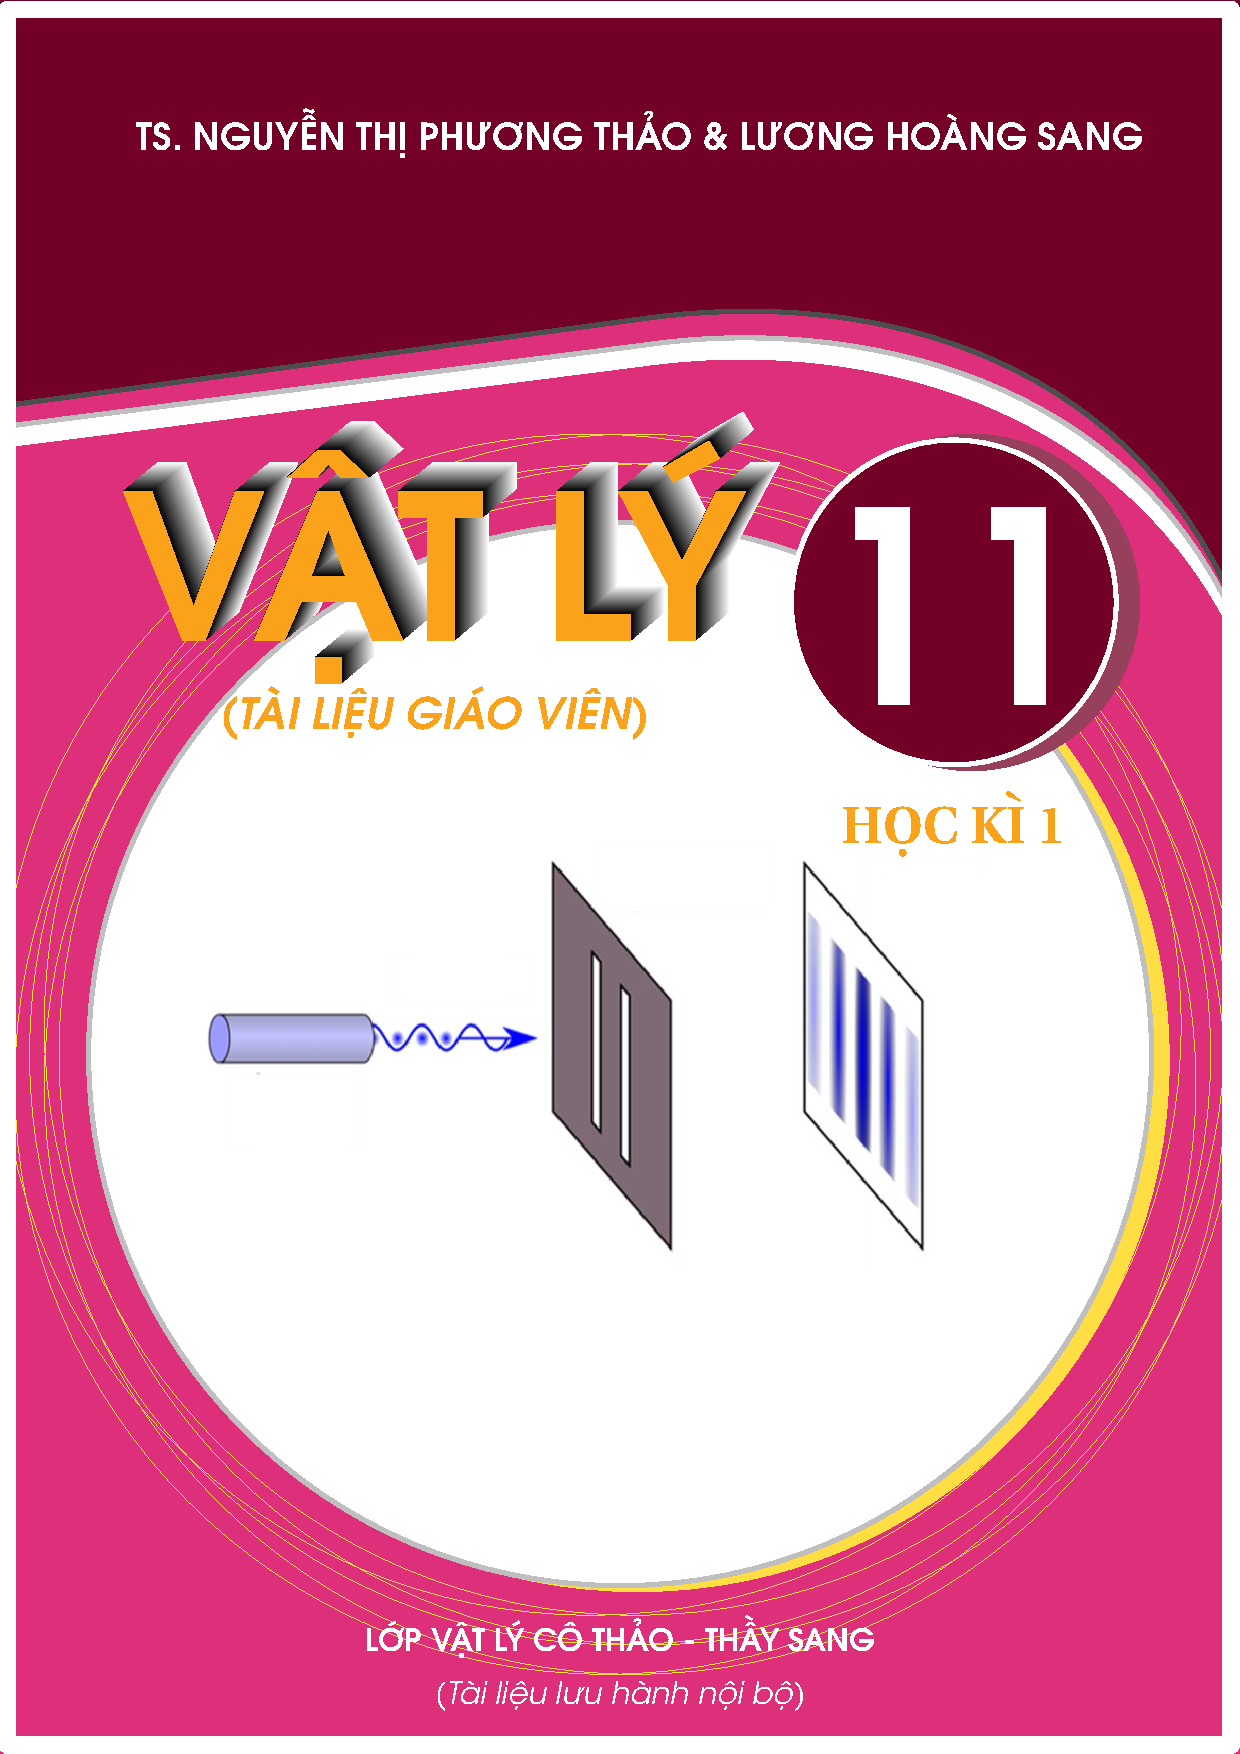
\includepdf{bia17/BIA11-HKI-GV.pdf}%chèn bìa pdf
%	\newpage\null\thispagestyle{empty}\newpage%tạo trang trống
	\clearpage%đặt lại đánh số trang
	%--Mục lục chính
	\FULLWIDTH
%	\muclucchinh%\cleardoublepage % tự động tạo trang trống ở vị trí chẵn
	\pagenumbering{arabic}%đánh số trang dạng 1,2,...
	%====================================================
	%==================BẮT ĐẦU TÀI LIỆU==================
	%==================Mục lục chính=====================
	\setcounter{part}{0}
	\setcounter{chapter}{0}
	\part{HỌC KỲ 1}%\cleardoublepage
%%%	CHƯƠNG 1: MỞ ĐẦU
	\chapter{MỞ ĐẦU}
\section{KHÁI QUÁT VỀ MÔN VẬT LÍ - VẤN ĐỀ AN TOÀN TRONG VẬT LÍ}
\subsection{LÝ THUYẾT TRỌNG TÂM}
\begin{tomtat}
	\subsubsection{ĐỐI TƯỢNG - MỤC TIÊU - PHƯƠNG PHÁP NGHIÊN CỨU VẬT LÍ}
	\paragraph{Đối tượng nghiên cứu của Vật lí}
	Đối tượng nghiên cứu của Vật lí gồm: các dạng vận động của \textbf{VẬT CHẤT} và \textbf{NĂNG LƯỢNG}.
	\paragraph{Mục tiêu nghiên cứu Vật lí}
	Mục tiêu của vật lí là khám phá ra quy luật tổng quát nhất chi phối sự vận động của vật chất và năng lượng cũng như tương tác giữa chúng ở mọi cấp độ: vi mô, vĩ mô.
	\paragraph{Phương pháp nghiên cứu Vật lí}
	\begin{dn}
		\textbf{\textit{Phương pháp thực nghiệm:}} dùng thí nghiệm để phát hiện kết quả mới giúp kiểm chứng, hoàn thiện, bổ sung hay bác bỏ giả thuyết nào đó. Kết quả mới này cần được giải thích bằng lí thuyết đã biết hoặc lí thuyết mới.
	\end{dn}
	\begin{dn}
		\textbf{\textit{Phương pháp lí thuyết:}} sử dụng ngôn ngữ toán học và suy luận lí thuyết để phát hiện một kết quả mới. Kết quả mới này cần được kiểm chứng bằng thực nghiệm.
	\end{dn}
	\begin{note}
		Hai phương pháp hỗ trợ cho nhau, trong đó phương pháp thực nghiệm có tính quyết định.
	\end{note}
	\paragraph{Quy trình tìm hiểu tự nhiên dưới góc độ Vật lí}
	\begin{center}
		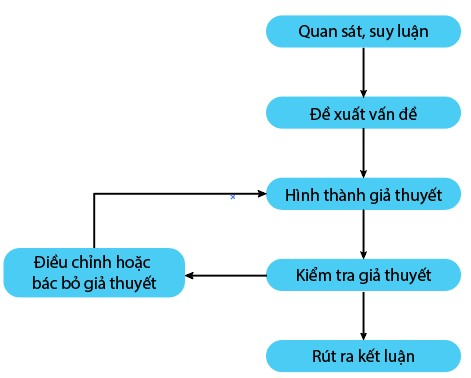
\includegraphics[scale=0.7]{figs/G10Y25B1-2}
	\end{center}
	\subsubsection{Quá trình phát triển của vật lí}
	\begin{center}
		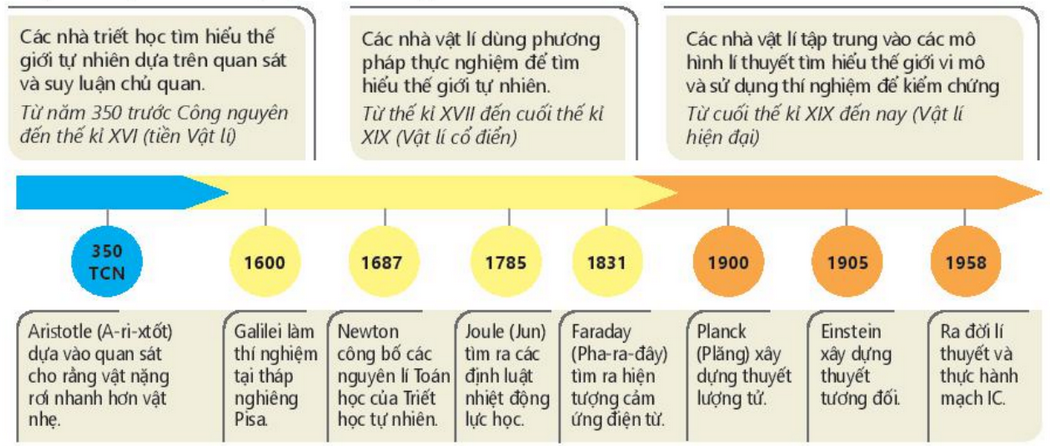
\includegraphics[scale=0.9]{figs/G10Y25B1-1}
	\end{center}
	\subsubsection{Vai trò của vật lí đối với khoa học, kĩ thuật và công nghệ}
	\paragraph{Thông tin liên lạc}
	Khoảng cách địa lí không còn là vấn đề quá lớn của con người trong thông tin liên lạc, sự bùng nổ của mạng lưới internet kết hợp sự phát triển vượt bậc của điện thoại thông minh (smartphone) giúp con người có thể chia sẻ thông tin liên lạc (hình ảnh, giọng nói, tin tức...) một cách dễ dàng.
	\paragraph{Y tế}
	Hầu hết các phương pháp chuẩn đoán và chữa bệnh trong y học đều có cơ sở từ những kiến thức Vật Lý như: chụp X – quang, chụp cộng hưởng từ (MRI), siêu âm, nội soi, xạ trị, \dots
	\paragraph{Công nghiệp}
	Cuộc cách mạng công nghiệp lần thứ tư được coi là bắt đầu thế kỉ XXI. Các nền sản xuất thủ công nhỏ lẻ được thay thế bởi những dây chuyền sản xuất tự động hóa, sử dụng trí tuệ nhân tạo, công nghệ vật liệu (nano), điện toán đám mây.
	\paragraph{Nông nghiệp}
	Việc ứng dụng những thành tựu của Vật Lý vào nông nghiệp đã giúp cho người nông dân tiếp cận với nhiều phương pháp mới, ít tốn lao động, cho năng suất cao. 
	\paragraph{Nghiên cứu khoa học}
	Vật lý góp phần to lớn trong việc cải tiến các thiết bị nghiên cứu khoa học ở nhiều ngành khác nhau như: kính hiển vi điện tử, nhiễu xạ tia X, máy quang phổ, \dots
\end{tomtat}
\subsubsection{Vấn đề an toàn trong Vật lí}
\paragraph{An toàn khi làm việc với phóng xạ}
\begin{enumerate}[label=\arabic*)]
	\item Giữ khoảng cách đủ xa đối với nguồn phóng xạ.
	\item Sử dụng các tấm chắn nguồn phóng xạ đủ tốt.
	\item Giảm thiểu thời gian phơi nhiễm phóng xạ.
\end{enumerate}
\begin{center}
	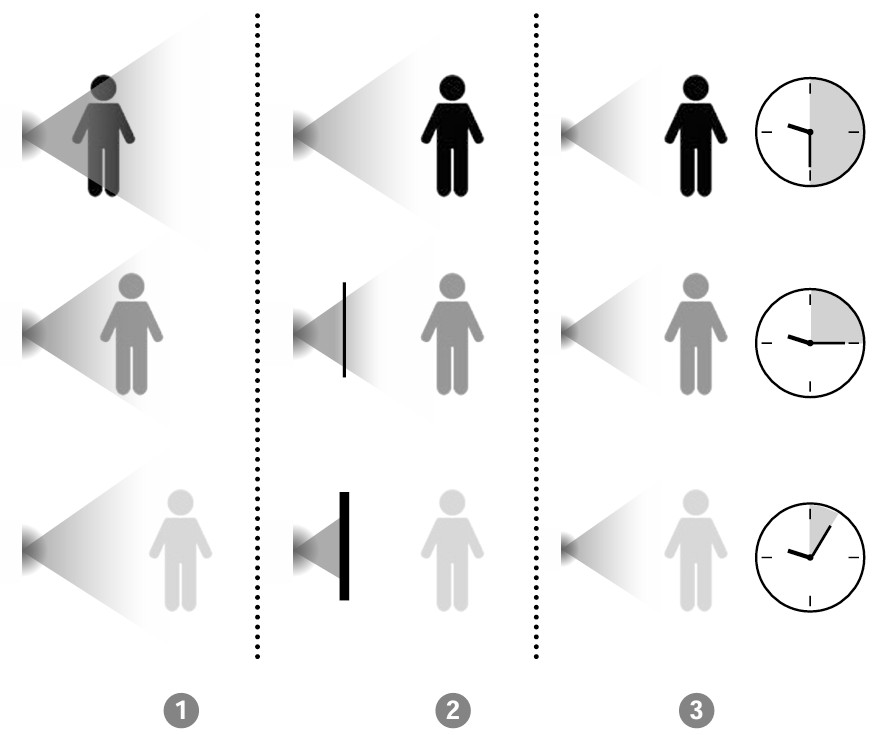
\includegraphics[scale=0.6]{figs/G10Y25B1-3}
\end{center}
\subsubsection{An toàn trong phòng thí nghiệm}
\begin{enumerate}[label=\alph*)]
	\item Một số biện pháp an toàn khi sử dụng điện:
	\begin{itemize}
		\item Trang bị đầy đủ các thiết bị bảo hộ cá nhân.
		\item Giữ khoảng cách an toàn với nguồn điện.
		\item Tránh sử dụng các thiết bị điện khi đang sạc.
		\item Không dùng tay ướt hoặc nhiều mồ hôi khi sử dụng dây điện.
		\item Tránh xa nơi điện thế nguy hiểm.
		\item Lắp đặt vị trí cầu dao, cầu chì, công tắc, ổ điện đúng quy định, \dots
	\end{itemize}
	\item  Khi nghiên cứu và học tập Vật lí cần phải:
	\begin{itemize}
		\item Hiểu được thông tin liên quan đến các rủi ro và nguy hiểm có thể xảy ra.
		\item Tuân thủ và áp dụng các biện pháp bảo vệ để đảm bảo an toàn cho bản thân và cộng đồng.
		\item Quan tâm, gìn giữ và bảo vệ môi trường.
		\item Trong phòng thí nghiệm ở trường học, những rủi ro và nguy hiểm phải được cảnh báo rõ ràng bằng các biển báo. Học sinh cần chú ý sự nhắc nhở của nhân viên phòng thí nghiệm và giáo viên về các quy định an toàn. Ngoài ra, các thiết bị bảo hộ cá nhân cần phải được trang bị đầy đủ.
	\end{itemize}
\end{enumerate}
\subsection{VÍ DỤ MINH HỌA}
\begin{dang}{Nêu được ví dụ về các phương pháp nghiên cứu vật lí}
\end{dang}
\begin{vd}
	Vào đầu thế kỉ XX, J.J.Thomson đã đề xuất mô hình cấu tạo nguyên tử gồm các electron phân bố đều trong một khối điện dương kết cấu tựa như khối mây. Để kiểm chứng giả thuyết này, E. Rutherford đã sử dụng tia alpha gồm các hạt mang điện dương bắn vào các nguyên tử kim loại vàng Hình \ref{fig:2.2}. Kết quả của thí nghiệm đã bác bỏ giả thuyết của J. J. Thomson, đồng thời đã giúp khám phá ra hạt nhân nguyên tử. E. Rutherford đã vận dụng phương pháp nghiên cứu nào để nghiên cứu vấn đề này? Giải thích.
	\begin{center}
		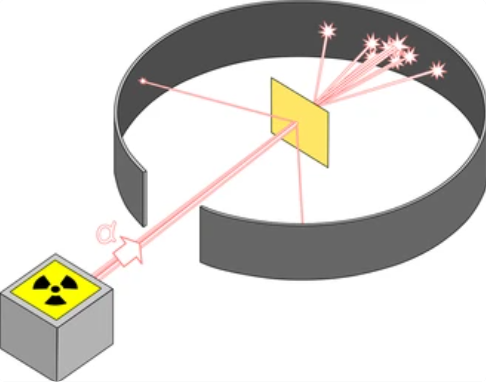
\includegraphics[scale=0.3]{figs/G10Y25B1-4}
		\captionof{figure}{Thí nghiệm Rutherford.}
		\label{fig:2.2}
	\end{center}
	\loigiai{
		Rutherford đã sử dụng phương pháp thực nghiệm trong nghiên cứu vật lí vì ông đã thực hiện thí nghiệm dùng tia alpha gồm các hạt mang điện dương bắn vào các nguyên tử vàng để phát hiện ra kết quả mới chính là hạt nhân nguyên tử.
	}
\end{vd}
\begin{dang}{Mô tả được các bước \\trong tiến trình tìm hiểu thế giới tự nhiên}
\end{dang}
\begin{vd}
	Sắp xếp các bước tiến hành quá trình tìm hiểu thế giới tự nhiên dưới góc độ vật lí:
	\begin{enumerate}[label= (\arabic*)]
		\item Phân tích số liệu.
		\item Quan sát, xác định đối tượng cần nghiên cứu.
		\item Thiết kế, xây dựng mô hình kiểm chứng giả thuyết.
		\item Đề xuất giả thuyết nghiên cứu.
		\item Rút ra kết luận.
	\end{enumerate}
	\loigiai{
		Tiến trình tìm hiểu thế giới tự nhiên dưới góc độ Vật lí là (2) - (4) - (3) - (1) - (5).
	}
\end{vd}
\begin{dang}{Vấn đề an toàn trong Vật lí}
\end{dang}
\begin{vd}
	Trạm không gian quốc tế ISS có độ cao khoảng \SI{400}{km}, trong khi bầu khí quyển có bề dày hơn \SI{100}{km}. Trong trạm không gian có tình trạng mất trọng lượng, mọi vật sẽ tự do lơ lửng. Hãy tìm hiểu các bất thường và nguy hiểm mà các nhà du hành làm việc lâu dài ở trong trạm có thể gặp phải.
	\loigiai{
	\begin{itemize}
		\item Không có tầng ozone bảo vệ, các phi hành gia dễ bị tia cực tím gây hại gây các bệnh về da.
		\item Mọi vật đều lơ lửng nên khó khăn trong sinh hoạt.
		\item Nguy hiểm từ các mảnh thiên thạch trôi nổi trong không gian.
		\item Ảnh hưởng sinh lí do sống lâu trong không gian.
	\end{itemize}
	}
	
\end{vd}

\subsection{TRẮC NGHIỆM NHIỀU PHƯƠNG ÁN LỰA CHỌN}
\setcounter{ex}{0}
\Opensolutionfile{ans}[ans/G10Y25B1-TN]
\begin{ex}
	Đối tượng nghiên cứu của Vật lí là gì?
	\choice
	{Các dạng vận động và tương tác của vật chất}
	{Quy luật tương tác của các dạng năng lượng}
	{\True Các dạng vận động của vật chất và năng lượng}
	{Quy luật vận động, phát triển của sự vật - hiện tượng}
	\loigiai{}
\end{ex}

\begin{ex}
	Lĩnh vực nghiên cứu nào sau đây là của Vật lí?
	\choice
	{Nghiên cứu về sự thay đổi của các chất khi kết hợp với nhau}
	{Nghiên cứu sự phát triển của vi khuẩn}
	{Nghiên cứu về sự hình thành và phát triển của các tầng lớp, giai cấp trong xã hội}
	{\True Nghiên cứu về các dạng chuyển động và các dạng năng lượng khác nhau}
	\loigiai{}
\end{ex}

\begin{ex}
	Cách sắp xếp nào sau đây trong 5 bước của phương pháp thực nghiệm là đúng?
	\choice
	{Xác định vấn đề cần nghiên cứu, dự đoán, quan sát, thí nghiệm, kết luận}
	{Quan sát, xác định vấn đề cần nghiên cứu, thí nghiệm, dự đoán, kết luận}
	{\True Xác định vấn đề cần nghiên cứu, quan sát, dự đoán, thí nghiệm, kết luận}
	{Thí nghiệm, xác định vấn đề cần nghiên cứu, dự đoán, quan sát, kết luận}
	\loigiai{}
\end{ex}

\begin{ex}
	Thành tựu nghiên cứu nào sau đây của Vật lí được coi là có vai trò quan trọng trong việc mở đầu cho cuộc cách mạng công nghệ lần thứ nhất?
	\choice
	{Nghiên cứu về lực vạn vật hấp dẫn}
	{\True Nghiên cứu về nhiệt động lực học}
	{Nghiên cứu về cảm ứng điện từ}
	{Nghiên cứu về thuyết tương đối}
	\loigiai{}
\end{ex}

\begin{ex}
	Từ việc quan sát sự rơi của các vật nặng nhẹ khác nhau mà Aristotle, một nhà khoa học Hy Lạp sống vào những năm 300 trước Công nguyên cho rằng: "Vật nặng rơi nhanh hơn vật nhẹ, vật càng nặng rơi càng nhanh". Yếu tố nào sau đây là quan trọng nhất dẫn tới việc Aristotle mắc sai lầm khi xác định nguyên nhân làm cho các vật rơi nhanh chậm khác nhau?
	\choice
	{Khoa học chưa phát triển}
	{Ông quá tự tin vào suy luận của mình}
	{Không có nhà khoa học nào khác giúp đỡ ông}
	{\True Ông không làm thí nghiệm để kiểm tra quan điểm của mình}
	\loigiai{}
\end{ex}

\begin{ex}
	Đối tượng nghiên cứu của vật lí là gì?
	\choice
	{Các dạng vận động và tương tác của vật chất}
	{Quy luật tương tác của các dạng năng lượng}
	{\True Các dạng vận động của vật chất và năng lượng}
	{Quy luật vận động, phát triển của sự vật hiện tượng}
	\loigiai{}
\end{ex}

\begin{ex}
	Mục tiêu của môn Vật lí là
	\choice
	{\True khám phá ra quy luật tổng quát nhất chi phối sự vận động của vật chất và năng lượng, cũng như tương tác giữa chúng ở mọi cấp độ: vi mô, vĩ mô}
	{khám phá ra quy luật tổng quát nhất chi phối sự vận động của vật chất và năng lượng}
	{khảo sát sự tương tác của vật chất ở mọi cấp độ: vi mô, vĩ mô}
	{khám phá ra quy luật vận động cũng như tương tác của vật chất ở mọi cấp độ: vi mô, vĩ mô}
	\loigiai{}
\end{ex}

\begin{ex}
	Cấp độ vi mô là
	\choice
	{\True cấp độ dùng để mô phỏng vật chất nhỏ bé}
	{cấp độ to, nhỏ tùy thuộc vào quy mô được khảo sát}
	{cấp độ dùng để mô phỏng tầm rộng lớn hay rất lớn của vật chất}
	{cấp độ tinh vi khi khảo sát một hiện tượng vật lí}
	\loigiai{}
\end{ex}

\begin{ex}
	Cấp độ vĩ mô là
	\choice
	{cấp độ dùng để mô phỏng vật chất nhỏ bé}
	{cấp độ to, nhỏ tùy thuộc vào quy mô được khảo sát}
	{\True cấp độ dùng để mô phỏng tầm rộng lớn hay rất lớn của vật chất}
	{cấp độ tinh vi khi khảo sát một hiện tượng vật lí}
	\loigiai{}
\end{ex}

\begin{ex}
	Chọn câu đúng khi nói về phương pháp thực nghiệm.
	\choice
	{Hai phương pháp thực nghiệm và lí thuyết hỗ trợ cho nhau, trong đó phương pháp lí thuyết có tính quyết định}
	{Phương pháp thực nghiệm sử dụng ngôn ngữ toán học và suy luận lí thuyết để phát hiện một kết quả mới}
	{\True Phương pháp thực nghiệm dùng thí nghiệm để phát hiện kết quả mới giúp kiểm chứng, hoàn thiện, bổ sung hay bác bỏ giả thuyết nào đó}
	{Kết quả được phát hiện từ phương pháp thực nghiệm cần được kiểm chứng bằng lí thuyết}
	\loigiai{}
\end{ex}

\begin{ex}
	Kết luận đúng về ảnh hưởng của vật lí đến một số lĩnh vực trong đời sống và kĩ thuật.
	\choice
	{Vật lí là cơ sở của khoa học tự nhiên và công nghệ}
	{Vật lí ảnh hưởng đến một số lĩnh vực: Thông tin liên lạc; Y tế; Công nghiệp; Nông nghiệp; Nghiên cứu khoa học}
	{Dựa trên nền tảng vật lí các công nghệ mới được sáng tạo với tốc độ vũ bão}
	{\True Tất cả đều đúng}
	\loigiai{}
\end{ex}

\begin{ex}
	Hiện tượng vật lí nào sau đây liên quan đến phương pháp thực nghiệm?
	\choice
	{Ô tô khi chạy đường dài có thể xem ô tô như là một chất điểm}
	{\True Thả rơi một vật từ trên cao xuống mặt đất}
	{Quả địa cầu là mô hình thu nhỏ của Trái đất}
	{Để biểu diễn đường truyền của ánh sáng người ta dùng tia sáng}
	\loigiai{}
\end{ex}

\begin{ex}
	Hiện tượng vật lí nào sau đây liên quan đến phương pháp lí thuyết?
	\choice
	{\True Ô tô khi chạy đường dài có thể xem ô tô như là một chất điểm}
	{Thả rơi một vật từ trên cao xuống mặt đất}
	{Kiểm tra sự thay đổi nhiệt độ trong quá trình nóng chảy hoặc bay hơi của một chất}
	{Ném một quả bóng lên trên cao}
	\loigiai{}
\end{ex}

\begin{ex}
	Những ngành nghiên cứu nào thuộc về vật lí
	\choice
	{\True Cơ học, nhiệt học, điện học và quang học}
	{Nhiệt học, quang học và sinh vật học}
	{Điện học, quang học và xã hội học}
	{Cơ học, nhiệt học và địa lý học}
	\loigiai{}
\end{ex}

\begin{ex}
	Ai được mệnh danh là “cha đẻ” của phương pháp thực nghiệm
	\choice
	{Isaac Newton}
	{\True Galileo Galilei}
	{Albert Einstein}
	{James Watt}
	\loigiai{}
\end{ex}

\begin{ex}
	Thành tựu nghiên cứu nào sau đây của Vật lí được coi là có vai trò quan trọng trong việc mở đầu cho cuộc cách mạng công nghiệp lần thứ hai vào cuối thế kỉ XIX?
	\choice
	{Nghiên cứu về lực vạn vật hấp dẫn}
	{Nghiên cứu về nhiệt động lực học}
	{\True Nghiên cứu về cảm ứng điện từ}
	{Nghiên cứu về thuyết tương đối}
	\loigiai{}
\end{ex}

\begin{ex}
	Đặc trưng cơ bản của cuộc cách mạng công nghiệp lần thứ ba ở thế kỉ XX là
	\choice
	{\True tự động hóa các quá trình sản xuất}
	{sự xuất hiện các thiết bị dùng điện trong mọi lĩnh vực sản xuất và đời sống con người}
	{thay thế sức lực cơ bắp bằng sức lực máy móc}
	{sử dụng trí tuệ nhân tạo, robot, internet toàn cầu, công nghệ vật liệu nano}
	\loigiai{}
\end{ex}

\begin{ex}
	Đặc trưng của cuộc cách mạng công nghiệp lần thứ tư vào đầu thế kỉ XXI là
	\choice
	{Xây dựng các dây chuyển sản suất tự động dựa trên những thành tựu nghiên cứu về điện tử,vi mạch, chất bán dẫn, ...}
	{\True Sử dụng trí tuệ nhân tạo, robot, internet toàn cầu, công nghệ vật liệu siêu nhỏ, điện thoại thông minh, ...}
	{Xuất hiện các thiết bị dùng điện trong mọi lĩnh vực sản xuất và đời sống con người}
	{Thay thế sức lực cơ bắp bằng sức lực máy móc}
	\loigiai{}
\end{ex}

\begin{ex}
	Chọn phát biểu chính xác nhất? Dự đoán khoa học là một dự đoán có cơ sở dựa trên yếu tố
	\choice
	{suy luận từ những hiện tượng khác có tính tương đồng}
	{quan sát, trải nghiệm thực tế}
	{\True quan sát, trải nghiệm thực tế, các kiến thức đã có liên quan đến dự đoán}
	{suy luận từ những thí nghiệm liên quan đến hiện tượng khác}
	\loigiai{}
\end{ex}

\begin{ex}
	Sau khi đưa ra một dự đoán khoa học thì người ta phải
	\choice
	{kết luận}
	{\True làm thí nghiệm để kiểm tra}
	{xác định vấn đề nghiên cứu}
	{tiếp tục đưa ra dự đoán mới}
	\loigiai{}
\end{ex}

\begin{ex}
	Khi nói về những quy tắc an toàn khi làm việc với phóng xạ, phát biểu nào sau đây là \textbf{sai}?
	\choice
	{Giảm thời gian tiếp xúc với nguồn phóng xạ}
	{Tăng khoảng cách từ ta đến nguồn phóng xạ}
	{Đảm bảo che chắn những cơ quan trọng yếu của cơ thể}
	{\True Mang áo phòng hộ và không cần đeo mặt nạ}
	\loigiai{}
\end{ex}

\begin{ex}
	Kí hiệu “Input (I)” mang ý nghĩa là
	\choice
	{cực dương}
	{cực âm}
	{\True đầu vào}
	{đầu ra}
	\loigiai{}
\end{ex}

\begin{ex}
	Chọn đáp án \textbf{sai}? Cần tuân thủ các biển báo an toàn trong phòng thực hành nhằm mục đích
	\choice
	{\True tạo ra nhiều sản phẩm mang lại lợi nhuận}
	{hạn chế các trường hợp nguy hiểm như: đứt tay, ngộ độc,…}
	{tránh được các tổn thất về tài sản nếu không làm theo hướng dẫn}
	{phòng chống cháy, nổ}
	\loigiai{}
\end{ex}

\begin{ex}
	Biển báo \vspace{-0.5cm}
\includegraphics[scale=0.1]{figs/G10Y25B1-5} mang ý nghĩa gì?\\
	\choice
	{\True Nơi nguy hiểm về điện}
	{Lưu ý cẩn thận}
	{Cẩn thận sét đánh}
	{Cảnh báo tia laser}
	\loigiai{}
\end{ex}

\begin{ex}
	Biển báo \vspace{-0.5cm}
\includegraphics[scale=0.2]{figs/G10Y25B1-6} mang ý nghĩa gì?\\
	\choice
	{Nơi cấm sử dụng quạt}
	{Tránh gió trực tiếp}
	{Lối thoát hiểm}
	{\True Nơi có chất phóng xạ}
	\loigiai{}
\end{ex}

\begin{ex}
	Chọn đáp án sai khi nói về những quy tắc an toàn trong phòng thí nghiệm.
	\choice
	{Đọc kĩ hướng dẫn sử dụng thiết bị và quan sát các chỉ dẫn, các kí hiệu trên các thiết bị thí nghiệm}
	{\True Tắt công tắc nguồn thiết bị điện sau khi cắm hoặc tháo thiết bị điện}
	{Kiểm tra cẩn thận thiết bị, phương tiện, dụng cụ thí nghiệm trước khi sử dụng}
	{Chỉ tiến hành thí nghiệm khi được sự cho phép của giáo viên hướng dẫn thí nghiệm}
	\loigiai{}
\end{ex}

\begin{ex}
	Chọn đáp án đúng khi nói về những quy tắc an toàn trong phòng thí nghiệm.
	\choice
	{Tắt công tắc nguồn thiết bị điện sau khi cắm hoặc tháo thiết bị điện}
	{Tuyệt đối không tiếp xúc với các vật và các thiết bị thí nghiệm có nhiệt độ cao ngay khi có dụng cụ bảo hộ}
	{Được phép tiến hành thí nghiệm khi đã mang đồ bảo hộ}
	{\True Phải vệ sinh, sắp xếp gọn gàng, các thiết bị và dụng cụ thí nghiệm, bỏ chất thải thí nghiệm vào đúng nơi quy định sau khi tiến hành thí nghiệm}
	\loigiai{}
\end{ex}

\begin{ex}
	Khi gặp sự cố mất an toàn trong phòng thực hành, học sinh cần
	\choice
	{\True báo cáo ngay với giáo viên trong phòng thực hành}
	{tự xử lí và không báo với giáo viên}
	{nhờ bạn xử lí sự cố}
	{tiếp tục làm thí nghiệm}
	\loigiai{}
\end{ex}

\begin{ex}
	Khi phòng thực hành xuất hiện cháy thì ta cần phải
	\choice
	{chạy ra khỏi phòng, đi tìm thêm người đến dập đám cháy}
	{\True ngắt điện, di chuyển các chất dễ cháy ra ngoài và chống cháy lan, cứu người, cứu tài sản, dập tắt đám cháy}
	{ngắt nguồn điện, dùng nước dập đám cháy}
	{dùng nước dập đám cháy}
	\loigiai{}
\end{ex}

\begin{ex}
	Trong bài thực hành có sử dụng mạch điện nhưng khi lắp ráp xong mạch điện, báo cáo giáo viên phụ trách rồi cắm vào nguồn điện nhưng mạch không vào điện thì học sinh cần
	\choice
	{kiểm tra lại mạch điện}
	{kiểm tra nguồn điện}
	{ngắt mạch điện ra khỏi nguồn}
	{\True ngắt mạch điện ra khỏi nguồn sau đó kiểm tra mạch điện và nguồn điện}
	\loigiai{}
\end{ex}

\subsection{TRẮC NGHIỆM ĐÚNG SAI}
\setcounter{ex}{0}
\begin{ex}
	Đối tượng nghiên cứu và mục tiêu của Vật lí:
	\choiceTF[t]
	{\True Đối tượng nghiên cứu của Vật lí gồm: các dạng vận động của vật chất và năng lượng}
	{\True Mục tiêu của Vật lí là khám phá ra quy luật tổng quát nhất chi phối sự vận động của vật chất và năng lượng, cũng như tương tác giữa chúng ở mọi cấp độ vi mô và vĩ mô}
	{Mục tiêu học tập môn Vật lí: Giúp học sinh hình thành, phát triển năng lực Toán học}
	{Cấp độ vĩ mô là là cấp độ dùng để mô phỏng vật chất nhỏ bé}
	\loigiai{\begin{itemchoice}
			\itemch Đúng.
			\itemch Đúng.
			\itemch Sai. Mục tiêu học tập môn Vật lí: Giúp học sinh hình thành, phát triển năng lực vật lí.
			\itemch Sai. Cấp độ vĩ mô là cấp độ dùng để mô phỏng tầm rộng lớn hay rất lớn của vật chất.
	\end{itemchoice}}
\end{ex}
\begin{ex}
	Quá trình phát triển của Vật lí trải qua 3 giai đoạn.
	\choiceTF[t]
	{\True Giai đoạn 1: Các nhà triết học tìm hiểu thế giới tự nhiên dựa trên quan sát và suy luận chủ quan: từ năm 350 trước Công nguyên đến thế kỉ XVI (tiền Vật lí)}
	{\True Giai đoạn 2: Các nhà vật lý dùng phương pháp thực nghiệm để tìm hiểu thế giới tự nhiên: từ thế kỉ XVII đến cuối thế kỉ XIX (Vật lí cổ điển)}
	{Giai đoạn 3: Các nhà vật lý tập trung vào các mô hình thực nghiệm tìm hiểu thế giới vĩ mô: Từ cuối thế kỉ XIX đến nay (Vật lí hiện đại)}
	{Việc ứng dụng các thành tựu của vật lý vào công nghệ luôn mang lại lợi ích cho nhân loại, không có tác hại gì}
	\loigiai{\begin{itemchoice}
			\itemch Đúng.
			\itemch Đúng.
			\itemch Sai. Giai đoạn 3: Các nhà vật lý tập trung vào các mô hình lí thuyết tìm hiểu thế giới \textbf{vi mô} và sử dụng thí nghiệm để kiểm chứng: Từ cuối thế kỉ XIX đến nay (Vật lí hiện đại).
			\itemch Sai. Việc ứng dụng các thành tựu của vật lý vào công nghệ không chỉ mang lại lợi ích cho nhân loại mà còn có thể làm ô nhiễm môi trường sống, hủy hoại hệ sinh thái,… nếu không được sử dụng đúng phương pháp, đúng mục đích.
	\end{itemchoice}}
\end{ex}
\begin{ex}
	Để đảm bảo an toàn trong phòng thí nghiệm, ta cần phải
	\choiceTF[t]
	{\True Nhờ giáo viên kiểm tra mạch điện trước khi bật nguồn điện}
	{Dùng tay ướt cắm điện vào nguồn điện}
	{\True Rửa sạch da khi tiếp xúc với hóa chất}
	{Để các thiết bị nối với nguồn điện giúp duy trì năng lượng}
	\loigiai{\begin{itemchoice}
			\itemch Đúng.
			\itemch Sai. 
			\itemch Đúng.
			\itemch Sai.
	\end{itemchoice}}
\end{ex}
\begin{ex}
	\immini{Hình bên là đồng hồ đa năng hiện số dùng để đo hiệu điện thế, cường độ dòng điện, điện trở,...
	\choiceTF
	{\True Điều chỉnh thang đo trên đồng hồ đa năng bằng cách vặn núm điều chỉnh ở giữa đồng hồ về vị trí cần tìm}
	{Vặn núm quay về bên trái để đo cường độ dòng điện}
	{\True Vặn núm quay về bên trái để đo hiệu điện thế}
	{Kí hiệu AC là dòng điện một chiều, DC là dòng điện xoay chiều}
	}
	{\vspace{-0.5cm}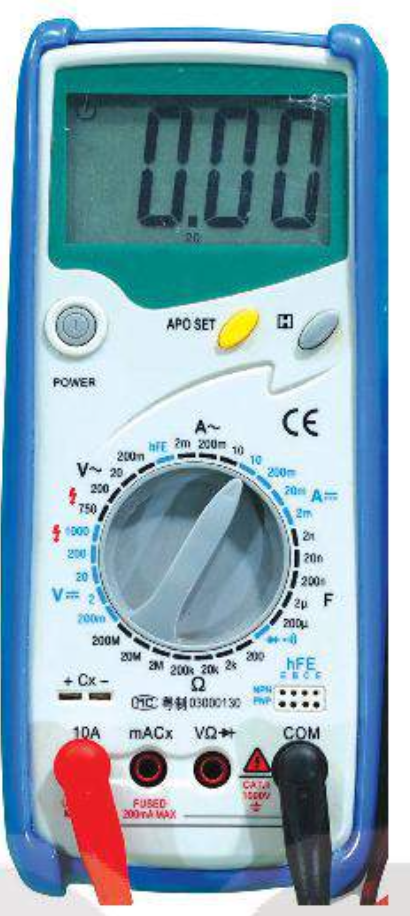
\includegraphics[scale=0.3]{figs/G10Y25B1-7}}
	
	\loigiai{\begin{itemchoice}
			\itemch Đúng.
			\itemch Sai. Vặn núm quay về bên phải.
			\itemch Đúng.
			\itemch Sai. Kí hiệu AC là dòng điện xoay chiều, DC là dòng điện một chiều.
	\end{itemchoice}}
\end{ex}

\subsection{TRẮC NGHIỆM TRẢ LỜI NGẮN}
\setcounter{ex}{0}

\begin{ex} 
	Quá trình phát triển của Vật lí trải qua bao nhiêu giai đoạn chính?
	\shortans[oly]{3}
	\loigiai{Tiền Vật lí, Vật lí cổ điển, Vật lí hiện đại}
\end{ex}
\begin{ex} 
	Lịch sử loài người đã trải qua bao nhiêu cuộc cách mạng công nghiệp dựa trên những kết quả nghiên cứu của Vật lí?
	\shortans[oly]{4}
	\loigiai{}
\end{ex}
\begin{ex} 
	Trong những hoạt động sau, có bao nhiêu hoạt động tuân thủ nguyên tắc an toàn khi làm việc với nguồn phóng xạ?
	\begin{enumerate}[label=\arabic*.]
		\item Sử dụng phương tiện phòng hộ cá nhân như quần áo phòng hộ, mũ, găng tay, áo chì.
		\item Ăn uống, trang điểm trong phòng làm việc có chứa chất phóng xạ.
		\item Tẩy xạ khi bị nhiễm bẩn phóng xạ theo quy định.
		\item Đổ rác thải phóng xạ tại các khu tập trung tác thải sinh hoạt.
		\item Mang nguồn phóng xạ về nhà luyện tập.
	\end{enumerate}
	\shortans[oly]{2}
	\loigiai{Hoạt động 1 và 3.}
\end{ex}
\begin{ex} 
	Có bao nhiêu biển báo mang ý nghĩa cảnh báo nguy hiểm trong hình bên dưới?
	\begin{center}
		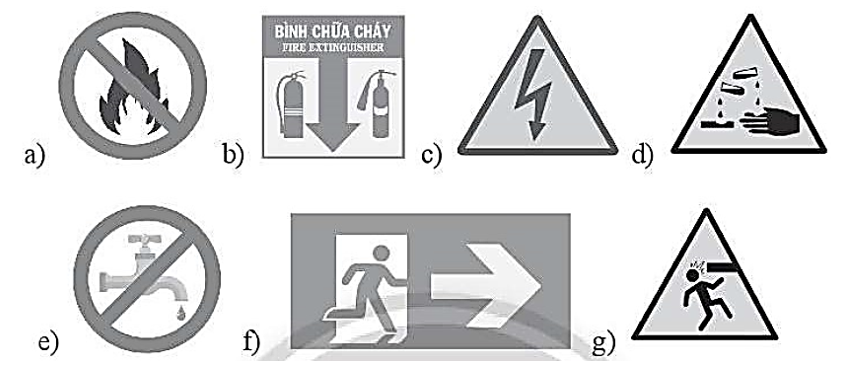
\includegraphics[scale=0.5]{figs/G10Y25B1-8}
	\end{center}
	\shortans[oly]{3}
	\loigiai{c, d và g.}
\end{ex}
\Closesolutionfile{ans}
\subsection{TỰ LUẬN}
\setcounter{ex}{0}
%\Opensolutionfile{ans}[ans/G10Y25B1-TL]
\begin{ex}
	Khi chiếu ánh sáng đến gương, ta quan sát thấy ánh sáng bị gương hắt trở lại môi trường cũ. Thực hiện những khảo sát chi tiết, ta có thể rút ra kết luận về nội dung định luật phản xạ ánh sáng như sau:\\
	-	Khi ánh sáng bị phản xạ, tia phản xạ sẽ nằm trong mặt phẳng chứa tia sáng tới và pháp tuyến của gương tại điểm tới.\\
	-	Góc phản xạ sẽ bằng góc tới.\\
	Hãy xác định đối tượng nghiên cứu và phương pháp nghiên cứu trong khảo sát trên.
	\loigiai{
	Đối tượng nghiên cứu: Sự truyền ánh sáng khi đến mặt gương.\\
	Phương pháp nghiên cứu: Phương pháp thực nghiệm.}
\end{ex}
\begin{ex}
	Cuộc cách mạng khoa học lần thứ nhất được đánh dấu bởi sự kiện khoa học nào? Đặc trưng của cuộc cách mạng khoa học lần thứ nhất là gì?
	\loigiai{
		Sự ra đời của động cơ hơi nước.\\
		Đặc trưng: thay thế sức lực của con người bằng sức lực của máy móc.}
\end{ex}
\begin{ex}
	Trình bày một số ví dụ minh họa cho phương pháp thực nghiệm trong Vật lí.
	\loigiai{
		Thí nghiệm tạo ra âm thanh (như gảy đàn, gõ vào thanh kim loại, ...) để chứng tỏ âm thanh truyền được trong chất rắn, lỏng, khí.\\
		Thí nghiệm sử dụng ánh sáng để đốt cháy tờ giấy, từ đó có thể nêu được ánh sáng có năng lượng.}
\end{ex}
\begin{ex}
	Tìm hiểu thực tế một số thiết bị vật lí dùng trong y tế để chẩn đoán, đo lường và chữa bệnh.
	\loigiai{
		\begin{enumerate}[label=\arabic*)]
			\item Các sợi quang dùng trong nội soi ứng dụng kiến thức về phản xạ toàn phần.
			\item Máy kích tim ứng dụng kiến thức về các tác dụng sinh lí của dòng điện.
			\item Máy chụp X quang.
			\item Máy đo tật khúc xạ của mắt ứng dụng kiến thức về định luật khúc xạ và thấu kính.
		\end{enumerate}
	}
\end{ex}
\begin{ex}
	Trình bày ví dụ chứng tỏ kiến thức Vật lí giúp tránh được nguy cơ tổn hại tài sản.
	\loigiai{
		Kiến thức về điện từ giúp mô tả được cách dòng điện chạy qua các mạch điện trong gia đình, hiểu được các phương pháp bảo vệ mạch điện, tránh được các vụ cháy nổ do chập điện...}
\end{ex}
\begin{ex}
	Ở những nơi nhiệt độ thấp (dưới \SI{0}{\celsius}), người ta nhận thấy rằng khi vung cùng một lượng nước nhất định ra không khí thì nước nóng sẽ đông đặc nhanh hơn so với nước lạnh. Em hãy xây dựng tiến trình tìm hiểu hiện tượng trên.
	\loigiai{
		\begin{enumerate}[label=Bước \arabic*:, leftmargin=2cm]
		\item \textit{Quan sát, suy luận:} “Nước nóng sẽ đông đặc nhanh hơn so với nước lạnh”.
		\item \textit{Đề xuất vấn đề:} Sự ảnh hưởng của nhiệt độ ban đầu đến thời gian đông đặc của nước.
		\item \textit{Hình thành giả thuyết:} Nước nóng sẽ đông đặc nhanh hơn so với nước lạnh.
		\item \textit{Kiểm tra giả thuyết:}\\
			Lập phương án thí nghiệm khảo sát thời gian đông đặc của hai cốc nước có nhiệt độ khác nhau khi cho vào ngăn đông của tủ lạnh.\\
			Tiến hành thí nghiệm. Pha hai cốc nước (cùng thể tích) có nhiệt độ 50C và 350C. Đặt 2 cốc nước và ngăn đông của tủ lạnh. Quan sát trạng thái đông đặc của hai cốc nước sau mỗi một giờ. Thu thập, xử lí và phân tích dữ liệu thực nghiệm.
		\item \textit{Rút ra kết luận}.
		\end{enumerate}
	}
\end{ex}
\begin{ex}
	Trong các hoạt động dưới đây, hoạt động nào dưới đây, hoạt động nào đảm bảo an toàn và những hoạt động nào gây nguy hiểm khi vào phòng thí nghiệm.
	\begin{enumerate}[label=\arabic*.]
		\item Mặc áo blouse, mang bao tay, kính bảo hộ trước khi vào phòng thí nghiệm.
		\item Nhờ giáo viên kiểm tra mạch điện trước khi bật nguồn điện.
		\item Dùng tay ướt cắm điện vào nguồn điện.
		\item Mang đồ ăn, thức uống vào phòng thí nghiệm.
		\item Thực hiện thí nghiệm nhanh và mạnh.
		\item Bỏ chất thải thí nghiệm vào đúng nơi quy định.
		\item Chạy nhảy, vui đùa trong phòng thí nghiệm.
		\item Rửa sạch da khi tiếp xúc với hóa chất.
		\item Tự ý đem đồ thí nghiệm mang về nhà luyện tập.
		\item Buộc tóc gọn gàng, tránh để tóc tiếp xúc với hóa chất và dụng cụ thí nghiệm.
	\end{enumerate}
	\loigiai{
		An toàn: 1, 2, 6, 8, 10.\\
		Nguy hiểm: 3, 4, 5, 7, 9.
	}
\end{ex}
\begin{ex}
	\immini {Trong quá trình thực hành tại phòng thí nghiệm, một bạn học sinh vô tình làm vỡ nhiệt kế thuỷ ngân và làm thuỷ ngân đổ ra ngoài như hình bên. Em hãy giúp bạn học sinh đó đưa ra cách xử lí thuỷ ngân đổ ra ngoài đúng cách để đảm bảo an toàn.}
	{\vspace{-0.75cm}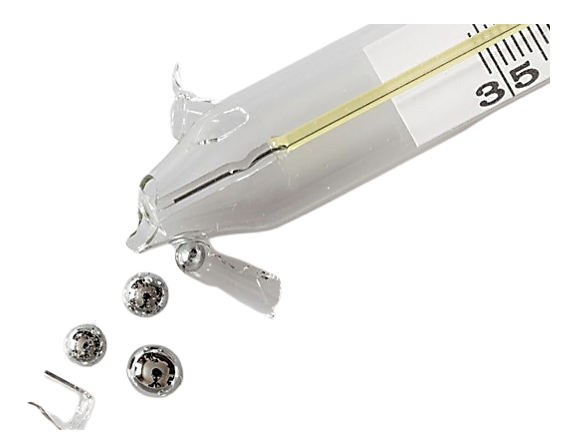
\includegraphics[scale=0.5]{figs/G10Y25B1-9}}
	\loigiai{Cách xử lí đúng nguyên tắc an toàn: báo cho giáo viên tại phòng thí nghiệm, sơ tán các bạn học sinh ở khu vực gần đó, tắt quạt và đóng hết cửa sổ để tránh việc thủy ngân phát tán trong không khí. Người dọn dẹp phải sử dụng găng tay và khẩu trang để dọn sạch thủy ngân, tuyệt đối không được tiếp xúc trực tiếp với thủy ngân bằng tay.}
\end{ex}
\begin{ex}
		\immini{Giới hạn đo của ampe kế ở hình bên là bao nhiêu? Nếu sử dụng ampe kế để đo dòng điện vượt quá giới hạn đo thì có thể gây ra nguy cơ gì?}
		{\vspace{-0.75cm}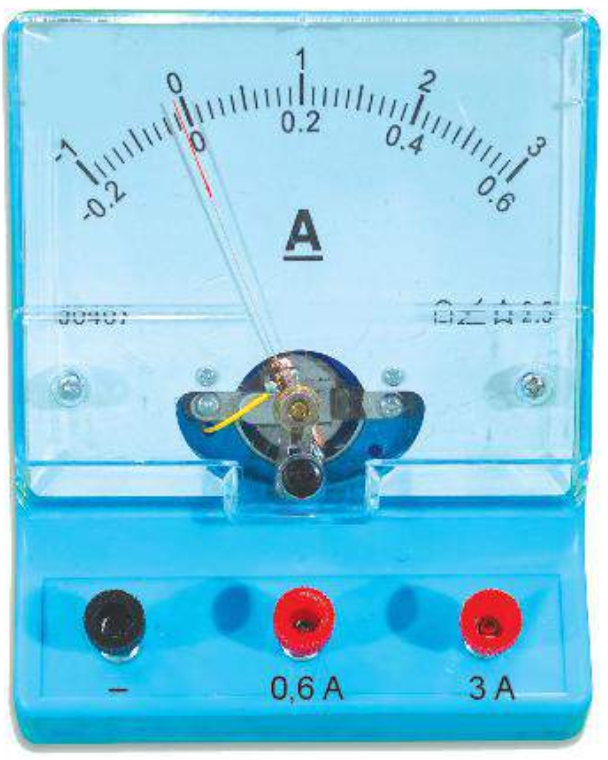
\includegraphics[scale=0.4]{figs/G10Y25B1-10}}
	\loigiai{
		Giới hạn đo là \SI{3}{A}.\\
		Nếu sử dụng ampe kế để đo dòng điện vượt quá giới hạn đo thì có thể làm cho ampe kế bị hư hỏng.
	}
\end{ex}
%\Closesolutionfile{ans}\newpage	% Hạnh (3t)
	\section{ĐƠN VỊ VÀ SAI SỐ TRONG VẬT LÍ}
\subsection{LÝ THUYẾT TRỌNG TÂM}
\begin{tomtat}
	\subsubsection{Đơn vị và thứ nguyên trong vật lí}
	\paragraph{Hệ đơn vị SI, đơn vị cơ bản và đơn vị dẫn xuất}
	\begin{dn}
		Tập hợp của đơn vị được gọi là hệ đơn vị. Trong khoa học có rất nhiều hệ đơn vị được sử dụng, trong đó thông dụng nhất là hệ đơn vị đo lường quốc tế SI (Système International d’unités) được xây dựng trên cơ sở của \textbf{7 đơn vị cơ bản}.
	\end{dn}
\begin{center}
	\captionof{table}{Các đơn vị cơ bản trong hệ SI}
	\begin{tabular}{|c|c|c|c|}
		\hline
		\thead{STT} & \thead{Đơn vị} & \thead{Kí hiệu} & \thead{Đại lượng}\\
		\hline
		$1$ & \text{mét} & $\si{\meter}$ & \text{Chiều dài}\\
		\hline
		$2$ & \text{kilôgam} & $\si{\kilo\gram}$ & \text{Khối lượng}\\
		\hline
		$3$ & \text{giây} & $\si{\second}$ & \text{Thời gian}\\
		\hline
		$4$ & \text{kelvin} & $\si{\kelvin}$ & \text{Nhiệt độ}\\
		\hline
		$5$ & \text{ampe}& $\si{\ampere}$ & \text{Cường độ dòng điện}\\ 
		\hline
		$6$ & \text{mol} & $\si{\mole}$ & \text{Lượng chất}\\
		\hline
		$7$ & \text{candela} & $\si{\candela}$ & \text{Cường độ sáng}\\
		\hline
	\end{tabular}
\end{center}
\begin{dn}
	\textbf{Đơn vị dẫn xuất:} Ngoài 7 đơn vị cơ bản, những đơn vị còn lại được gọi là đơn vị dẫn xuất. \\Mọi đơn vị dẫn xuất đều có thể phân tích thành các đơn vị cơ bản dựa vào mối liên hệ giữa các đại lượng tương ứng.
\end{dn}
\paragraph{Thứ nguyên}
Thứ nguyên của một đại lượng là quy luật nêu lên sự phụ thuộc của đơn vị đo đại lượng đó vào các đơn vị cơ bản.
\begin{itemize}
	\item Thứ nguyên của một đại lượng $X$ được biễn diễn dưới dạng $[X]$. Thứ nguyên của một số đại lượng cơ bản thường sử dụng được thể hiện trong Bảng \ref{tab:2}.
	\item Một đại lượng vật lí có thể được biểu diễn bằng nhiều đơn vị khác nhau nhưng chỉ có một thứ nguyên duy nhất. Một số đại lượng vật lí có thể có cùng thứ nguyên.
\end{itemize}
\begin{center}
	\captionof{table}{Thứ nguyên của một số đại lượng cơ bản}
	\label{tab:2}
	\begin{tabular}{|c|c|}
		\hline
		\thead{Đại lượng cơ bản} & \thead{Thứ nguyên}\\
		\hline
		\text{[Chiều dài]} & $L$\\
		\hline
		\text{[Khối lượng]} & $M$\\
		\hline
		\text{[Thời gian]} & $T$\\
		\hline
		\text{[Cường độ dòng điện]} & $I$\\
		\hline
		\text{[Nhiệt độ]} & $K$\\
		\hline
	\end{tabular}
\end{center}
\begin{luuy}
	Trong các biểu thức vật lí:
	\begin{itemize}
		\item Các số hạng trong phép cộng (hoặc trừ) phải có cùng thứ nguyên.
		\item Hai vế của một biểu thức vật lí có cùng thứ nguyên.
	\end{itemize}
\end{luuy}
\paragraph{Tên và kí hiệu các tiếp đầu ngữ của bội số, ước số thập phân của đơn vị}
	Khi số đo của đại lượng đang xem xét là một bội số hoặc ước số thập phân của mười, ta có thể sử dụng tiếp đầu ngữ như trong Bảng \ref{tab:1} ngay trước đơn vị để phần số đo được trình bày ngắn gọn.
	\begin{center}
		\captionof{table}{Tên và kí hiệu tiếp đầu ngữ của bội số, ước số thập phân của đơn vị}
		\begin{tabular}{|c|c|c|c|c|c|}
			\hline
			\thead{Kí hiệu} & \thead{Tên đọc} & \thead{Hệ số} & \thead{Kí hiệu} & \thead{Tên đọc} & \thead{Hệ số}\\
			\hline
			Y & \text{yotta} & $10^{24}$ & \text{y} & \text{yokto} & $10^{-24}$\\
			\hline
			Z & \text{zetta} & $10^{21}$ & z & \text{zepto} & $10^{-21}$\\
			\hline
			E & \text{eta} & $10^{18}$ & \text{a} & \text{atto} & $10^{-18}$\\
			\hline
			P & \text{peta} & $10^{15}$ & f & \text{femto} & $10^{-15}$\\
			\hline
			T & \text{tera} & $10^{12}$ & p & \text{pico} & $10^{-12}$\\
			\hline
			G & \text{giga} & $10^{9}$ & n & \text{nano} & $10^{-9}$\\
			\hline
			M & \text{mega} & $10^{6}$ & \text{$\mu$} & \text{micro} & $10^{-6}$\\
			\hline
			k & \text{kilo} & $10^{3}$ & m & \text{mili} & $10^{-3}$\\
			\hline
			h & \text{hecto} & $10^{2}$ & c & \text{centi} & $10^{-2}$\\
			\hline
			da & \text{deka} & $10^{1}$ & d & \text{deci} & $10^{-1}$\\
			\hline
		\end{tabular}
		\label{tab:1}
	\end{center}
	
	\subsubsection{Sai số trong phép đo và cách hạn chế}
	\paragraph{Phép đo các đại lượng vật lí}
	Phép đo một đại lượng vật lí là phép so sánh nó với đại lượng cùng loại được quy ước làm đơn vị.\\	
	Phép đo được phân loại thành 
	\begin{itemize}
		\item \textbf{Phép đo trực tiếp} là phép xác định giá trị  một đại lượng bằng cách so sánh trực tiếp với dụng cụ đo (ví dụ như đo khối lượng bằng cân, đo nhiệt độ bằng nhiệt kế). 
		\item \textbf{Phép đo gián tiếp} là phép xác định giá trị một đại lượng thông qua một công thức liên hệ với các đại lượng được đo trực tiếp (ví dụ như đo khối lượng riêng thông qua việc xác định khối lượng và thể tích của khối vật chất).   
	\end{itemize}
	\paragraph{Các loại sai số của phép đo}
	\begin{center}
		\captionof{table}{Các loại sai số của phép đo}
		\begin{longtable}{|m{5em}|m{7.5cm}|m{7.5cm}|}
			\hline
			&\thead{Sai số hệ thống} & \thead{Sai số ngẫu nhiên}\\
			\hline
			\thead{Khái\\ niệm} & Sai số hệ thống là sai số có tính quy luật và được lặp lại ở tất cả các lần đo. Sai số hệ thống làm cho giá trị đo tăng hoặc giảm một lượng nhất định so với giá trị thực. & Sai số ngẫu nhiên là sai số xuất phát từ sai sót, phản xạ của người làm thí nghiệm hoặc từ những yếu tố ngẫu nhiên bên ngoài.\\
			\hline
			\thead{Nguyên\\ nhân} & Các dụng cụ đo các đại lượng vật lí luôn có sự sai lệch do đặc điểm và cấu tạo của dụng cụ gây ra. & Sai số này thường có nguyên nhân không rõ ràng và dẫn đến sự phân tán của các kết quả đo xung quanh một giá trị trung bình.\\
			\hline
			\thead{Cách\\ hạn chế} & Sai số hệ thống có thể được hạn chế bằng cách thường xuyên hiệu chỉnh dụng cụ đo, sử dụng thiết bị đo có độ chính xác cao. & Sai số ngẫu nhiên có thể được hạn chế bằng cách thực hiện phép đo nhiều lần và lấy giá trị trung bình để hạn chế sự phân tán của số liệu đo.\\
			\hline
		\end{longtable}
	\end{center}
	\begin{luuy}
		Đối với một số dụng cụ đo, sai số dụng cụ thường được xác định bằng một nửa độ chia nhỏ nhất.
	\end{luuy}
	\subsubsection{Biểu diễn kết quả đo}
	\paragraph{Cách biểu diễn sai số của phép đo}
	Khi đo $n$ lần cùng một đại lượng $A$, ta thu được các giá trị khác nhau: $A_1,\, A_2,\,...,A_n$\\
	Giá trị trung bình khi đo nhiều lần một đại lượng $A$:$$\bar{A}=\dfrac{A_1+A_2+...+A_{\text{n}}}{n},$$
	là giá trị gần đúng nhất với giá trị thực của đại lượng $A$.  
	\begin{itemize}
		\item Sai số tuyệt đối ứng với mỗi lần đo:
		$$\Delta A_1=|\bar{A}-A_1|;\quad\Delta A_2=|\bar{A}-A_2|;\quad\Delta A_3=|\bar{A}-A_3|;\dots; \Delta A_i=\left|\overline{A}-A_i\right|$$
		\item Sai số ngẫu nhiên là sai số tuyệt đối trung bình của $n$ lần đo:
		$$\overline{\Delta A}=\dfrac{\Delta A_1+\Delta A_2+...+\Delta A_{\textrm{n}} }{n}.$$
		\item Sai số dụng cụ $\Delta A_\text{dc}$ thường được lấy bằng nửa độ chia nhỏ nhất đối với những dụng cụ đơn giản như thước kẻ, cân bàn, bình chia độ, \dots Trong nhiều trường hợp, sai số dụng cụ thường được cung cấp chính xác bởi nhà sản xuất.
		\item Sai số tuyệt đối của phép đo cho biết phạm vi biến thiên của giá trị đo được và bằng tổng của sai số ngẫu nhiên và sai số dụng cụ:
		$$\Delta A= \overline{\Delta A}+ \Delta A_\text{dc}.$$
	\end{itemize}
	\paragraph{Sai số tương đối (tỉ đối)}
	Sai số tỉ đối $\delta A$ của phép đo là tỉ số giữa \textbf{sai số tuyệt đối} và \textbf{giá trị trung bình} của đại lượng cần đo, tính bằng phần trăm:
	$$\delta A=\dfrac{\Delta A}{\overline A}\cdot 100\%.$$
	Sai số tỉ đối càng \textbf{nhỏ} thì phép đo càng chính xác.
	\paragraph{Cách xác định sai số của phép đo gián tiếp}
	Sai số của phép đo gián tiếp, được xác định theo các quy tắc:
	\begin{itemize}
		\item Sai số tuyệt đối của một tổng hay hiệu thì bằng \textbf{tổng} các sai số tuyệt đối của các số hạng:\\
		Nếu $F=x\pm y\pm z \dots$ thì $\Delta F = \Delta x + \Delta y + \Delta z+\dots$.
		\item Sai số tỉ đối của một tích hay thương thì bằng \textbf{tổng} các sai số tỉ đối của các thừa số:\\ 
		Nếu $F= x^m\cdot\dfrac{y^n}{z^k}$ thì $\delta F=m\cdot\delta x+n\cdot\delta y +k\cdot\delta z$.
	\end{itemize}
	\begin{noidung}{Quy tắc xác định số chữ số có nghĩa (CSCN):}
			Các chữ số có nghĩa bao gồm:
		\begin{itemize}
			\item Các chữ số khác 0.
			\item Các chữ số 0 nằm giữa hai chữ số khác 0.
			\item Các chữ số 0 nằm bên phải của dấu	thập phân và một chữ số khác 0
		\end{itemize}
	\end{noidung}
	\textit{Ví dụ:} \textbf{678} có ba chữ số có nghĩa, \textbf{6008} có bốn chữ số có nghĩa, 0,0\textbf{800} có ba chữ số có nghĩa.
	\paragraph{Cách viết kết quả đo}
	$$A=\overline{A} \pm \Delta A,$$
	trong đó:
	\begin{itemize}
		\item $\overline A$ là giá trị trung bình,
		\item $\Delta A$ là sai số tuyệt đối. 
	\end{itemize}
\end{tomtat}
\subsection{VÍ DỤ MINH HỌA}
\begin{dang}{Tìm hiểu một số loại sai số đơn giản hay gặp khi đo các đại lượng vật lí và cách khắc phục chúng}
	\end{dang}
	\begin{vd}
		Quan sát các hình sau và phân tích các nguyên nhân gây ra sai số của phép đo trong các trường hợp được nêu
		\begin{center}
			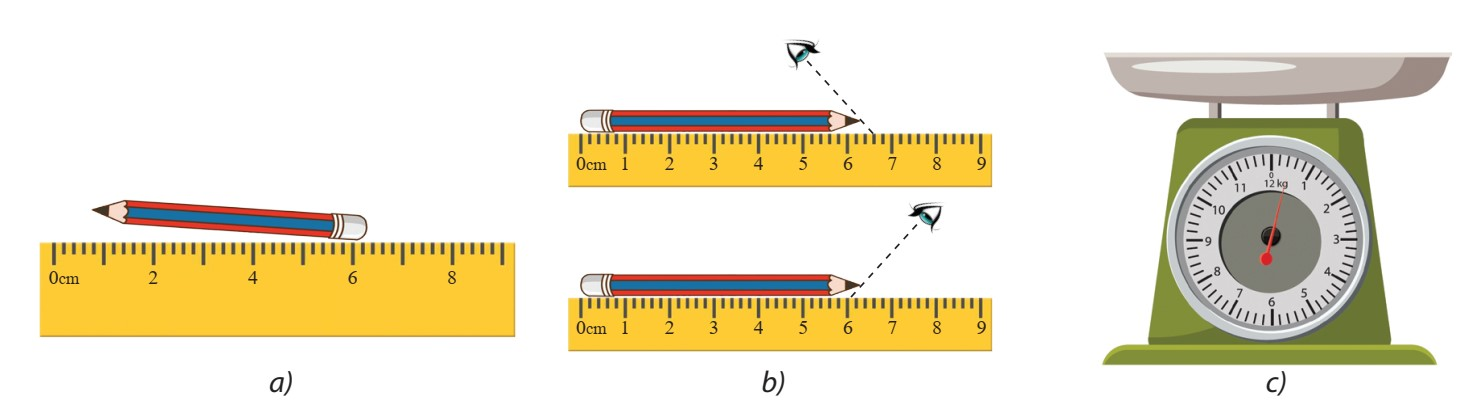
\includegraphics[scale=0.5]{figs/G10Y25B2-1}
		\end{center}
		\loigiai{
			\begin{enumerate}[label=\alph*)]
				\item Đặt bút không dọc theo thước, đầu bút không trùng với vạch số 0.
				\item Đặt mắt sai cách, hướng nhìn không vuông góc.
				\item Kim cân chưa được hiệu chỉnh về số 0.
			\end{enumerate}
		}
	\end{vd}
\begin{dang}{Vận dụng mối liên hệ giữa đơn vị dẫn xuất với 7 đơn vị cơ bản của hệ SI}
\end{dang}
\begin{vd}
	Để xác định quãng đường đi được $s$ của một chất điểm chuyển động thẳng đều, một bạn học sinh đã viết công thức như sau: $s=\alpha\cdot v\cdot t^2$ với $v$ và $t$ lần lượt là vận tốc và thời gian, $\alpha$ là hằng số không thứ nguyên. Dựa vào việc xác định thứ nguyên, em hãy cho biết công thức trên là đúng hay sai.
	\loigiai{
		Thứ nguyên của các đại lượng $s$, $v$ và $t$ lần lượt là
		\begin{itemize}
			\item $\left[s\right]=L$
			\item $\left[v\right]=L\cdot T^{-1}$
			\item $\left[t\right]=T$
		\end{itemize}
		Từ đó, ta thấy vế trái của công thức trên có thứ nguyên $L$ trong khi vế phải lại có thứ nguyên $L\cdot T$. Do 2 vế của công thức không cùng thứ nguyên nên bạn học sinh chưa đưa ra được công thức chính xác.
		Dựa vào phân tích thứ nguyên, ta cần sửa lại công thức chính xác như sau:
		$$s=\alpha \cdot v\cdot t$$
		Trong hệ SI, $s$, $v$ và $t$ lần lượt có đơn vị là $\si{\meter}, \si{\meter\cdot\second^{-1}}, \si{\second}$.
	}
\end{vd}
\begin{dang}{Xác định được sai số tuyệt đối, sai số tỉ đối và biểu diễn được kết quả đo}
\end{dang}
\begin{vd}
	Cho bảng số liệu thể hiện kết quả đo đường kính của một viên bi thép bằng thước kẹp có sai số dụng cụ là $\SI{0.02}{\milli\meter}$. Tính sai số tuyệt đối, sai số tương đối của phép đo và biểu diễn kết quả đo có kèm theo sai số
	\begin{longtable}{|c|c|c|}
		\hline
		\thead{Lần đo} & \thead{$d \left(\si{\milli\meter}\right)$} & \thead{$\Delta d \left(\si{\milli\meter}\right)$}\\
		\hline
		1 & 6,32 & \dots\\
		\hline
		2 & 6,32 & \dots\\
		\hline
		3 & 6,32 & \dots\\
		\hline
		4 & 6,32 & \dots\\
		\hline
		5 & 6,34 & \dots\\
		\hline
		6 & 6,34 & \dots\\
		\hline
		7 & 6,32 & \dots\\
		\hline
		8 & 6,34 & \dots\\
		\hline
		9 & 6,32 & \dots\\
		\hline
		\textbf{Trung bình} & $\overline{d}=?$ & $\overline{\Delta d}=?$\\
		\hline
	\end{longtable}
	
	\loigiai{
		Giá trị trung bình của đường kính viên bi:
		$$\overline{d}=\dfrac{d_1+d_2+d_3+\dots+d_9}{9}\approx\SI{6.327}{\milli\meter}$$
		Sai số tuyệt đối ứng với mỗi lần đo
		$$\Delta d_i=\left|\overline{d}-d_i\right|$$
		$$\Delta d_1=\Delta d_2=\Delta d_3=\Delta d_4=\Delta d_7=\Delta d_9=\left|\SI{6.327}{\milli\meter}-\SI{6.32}{\milli\meter}\right|=\SI{0.007}{\milli\meter}$$
		$$\Delta d_5=\Delta d_6=\Delta d_8=\left|\SI{6.327}{\milli\meter}-\SI{6.34}{\milli\meter}\right|=\SI{0.013}{\milli\meter}$$
		Sai số tuyệt đối trung bình của phép đo:
		$$\overline{\Delta d}=\dfrac{\Delta d_1+\Delta d_2+\dots+\Delta d_9}{9}=\SI{0.009}{\milli\meter}$$
		Sai số tuyệt đối của phép đo:
		$$\Delta d = \overline{\Delta d}+\Delta d_\text{dc}=\SI{0.009}{\milli\meter}+\SI{0.02}{\milli\meter}=\SI{0.029}{\milli\meter}$$
		Sai số tương đối của phép đo:
		$$\delta d =\dfrac{\Delta d}{\overline{d}}\cdot\SI{100}{\percent}\approx\SI{0.46}{\percent}$$
		Kết quả phép đo:
		$$d=\overline{d}\pm\Delta d=\SI{6.273}{\milli\meter}\pm\SI{0.029}{\milli\meter}.$$
	}
\end{vd}

\begin{vd}
	Trong bài thực hành đo gia tốc trọng trường của Trái Đất tại phòng thí nghiệm, một học sinh đo được chiều dài của con lắc đơn $\ell= \xsi{800\pm 1}{\milli\meter}$ thì chu kì dao động là $T = \xsi{1.78\pm 0.02}{\second}$. Lấy $\pi=\SI{3.14}{}$. Biết chu kỳ của con lắc đơn tính theo công thức $T=2\pi \sqrt{\dfrac{\ell}{g}}$. Gia tốc trọng trường $g$ của Trái Đái tại phòng thí nghiệm đó là bao nhiêu?
	\loigiai{
		Từ công thức: $$T=2\pi \sqrt{\dfrac{\ell}{g}} \Rightarrow g=\dfrac{4\pi^2\ell}{T^2}.$$ 	
		
		Giá trị trung bình của gia tốc trọng trường: 	
		$$\overline{g}=\dfrac{4\pi^2\ell}{T^2}=\dfrac{4\pi^2\cdot \SI{3.14}{}\cdot \SI{0.8}{\meter}}{\left( \SI{1.78}{\second}\right)^2}=\SI{9.96}{\meter\per\second^2}.$$
		
		Sai số tuyệt đối của gia tốc trọng trường:
		\begin{align*}
			\dfrac{\Delta g}{\overline g}&= \dfrac{\Delta \ell}{\overline \ell}+ 2\dfrac{\Delta T}{\overline T}\\
			&=\dfrac{\SI{1}{\milli\meter}}{\SI{800}{\milli\meter}}+2\times\dfrac{\SI{0.02}{\second}}{\SI{1.78}{\second}}\\
			&=\SI{0.024}{}\\
			\Rightarrow\quad \Delta g&= \SI{0.024}{}\cdot \overline g\\
			&= \SI{0.24}{\meter\per\second^2}.
		\end{align*}
		
		
		
		Vậy gia tốc trọng trường của Trái Đất tại phòng thí nghiệm đó là
		$$g={\overline g } \pm \Delta g =\SI{9.96}{\meter\per\second^2}\pm\SI{0.24}{\meter\per\second^2}.$$
	}
\end{vd}

\begin{vd}
	Một học sinh dùng cân và đồng hồ đếm giây để đo độ cứng $k$ của lò xo. Dùng cân để cân vật nặng thu được kết quả khối lượng $m = \SI{100}{\gram}$ với sai số tỉ đối là $\SI{2}{\percent}$. Gắn vật vào lò xo và kích thích cho con lắc dao động rồi dùng đồng hồ đếm giây đo thời gian của một dao động cho kết quả $T = \SI{2}{\second}$ với sai số tỉ đối là $\SI{1}{\percent}$. Biết chu kỳ của con lắc lò xo tính theo công thức $T=2\pi \sqrt{m/k}$. Sai số tỉ đối của phép đo độ cứng của lò xo là bao nhiêu?
	\loigiai{
		Từ công thức: $$T=2\pi \sqrt{\dfrac{m}{k}} \Rightarrow k=\dfrac{4\pi^2m}{T^2}.$$	
		
		Sai số tỉ đối của độ cứng lò xo: 	
		$$\dfrac{\Delta k}{\overline k}= \dfrac{\Delta m}{\overline m}+ 2\dfrac{\Delta T}{\overline T}= \SI{2}{\percent}+2\cdot \SI{1}{\percent}= \SI{4}{\percent}.$$
		
		Vậy sai số tỉ đối của phép đo độ cứng của lò xo là $\SI{4}{\percent}.$
	}
\end{vd}
\subsection{TRẮC NGHIỆM NHIỀU PHƯƠNG ÁN LỰA CHỌN}
\setcounter{ex}{0}
\Opensolutionfile{ans}[ans/G10Y25B2-TN]
\begin{ex}
	Hệ đơn vị đo lường quốc tế SI được xây dựng dựa trên mấy đơn vị cơ bản?
	\choice
	{5}
	{6}
	{\True 7}
	{8}
	\loigiai{}
\end{ex}

\begin{ex}
	Trong các đại lượng sau, đại lượng nào \textbf{không phải} đại lượng cơ bản trong hệ SI?
	\choice
	{Chiều dài}
	{Thời gian}
	{Khối lượng}
	{\True Lực}
	\loigiai{}
\end{ex}

\begin{ex}
	Tiếp đầu ngữ “kilo” có nghĩa là
	\choice
	{$10^{-3}$}
	{\True $10^{3}$}
	{$10^{-6}$}
	{$10^{6}$}
	\loigiai{}
\end{ex}

\begin{ex}
	Trong các đại lượng sau, đại lượng nào \textbf{không phải} đại lượng cơ bản trong hệ SI?
	\choice
	{Chiều dài}
	{Thời gian}
	{Khối lượng}
	{\True Lực}
	\loigiai{}
\end{ex}

\begin{ex}
	Đáp án nào sau đây có 1 đơn vị cơ bản và 1 đơn vị dẫn xuất?
	\choice
	{mét, kilogram}
	{\True newton, mol}
	{pascal, joule}
	{candela, kelvin}
	\loigiai{}
\end{ex}

\begin{ex}
	Đơn vị đo nhiệt độ trong hệ SI là
	\choice
	{$\si{\celsius}$}
	{$^\circ$F}
	{\True K}
	{cal}
	\loigiai{}
\end{ex}

\begin{ex}
	Trong các tiếp đầu ngữ sau, tiếp đầu ngữ nào có giá trị lớn nhất
	\choice
	{Mega}
	{Giga}
	{Kilo}
	{\True Tera}
	\loigiai{}
\end{ex}

\begin{ex}
	Trong hệ đơn vị SI, tốc độ có đơn vị là
	\choice
	{$\si{\kilo\meter/\hour}$}
	{\True $\si{\meter/\second}$}
	{$\si{\text{dặm}/\hour}$}
	{$\si{ft/\second}$}
	\loigiai{}
\end{ex}

\begin{ex}
	Thứ nguyên của vận tốc là
	\choice
	{$LT$}
	{$L^{-1}T$}
	{$L^{-1}T^{-1}$}
	{\True $LT^{-1}$}
	\loigiai{
		\begin{align*}
			v&=\dfrac{s}{t}\\
			\Rightarrow \left[v\right]&=\dfrac{\left[s\right]}{\left[t\right]}=LT^{-1}.
		\end{align*}
	}
\end{ex}

\begin{ex}
	Đơn vị nào sau đây không thuộc thứ nguyên $L$ [Chiều dài]?
	\choice
	{Dặm}
	{Hải lí}
	{Năm ánh sáng}
	{\True Năm}
	\loigiai{}
\end{ex}

\begin{ex}
	Trong các biểu thức sau, biểu thức nào \textbf{không đồng nhất} về thứ nguyên?
	\choice
	{$E = \dfrac{qV}{2}$}
	{$v = \omega r$}
	{\True $s = vt^{2}$}
	{$T = 2\pi\sqrt{\dfrac{l}{g}}$}
	\loigiai{
		Vế phải của $s = vt^{2}$ có thứ nguyên $LT^{-1}\,T^{2}=LT\;\neq\;L$ của vế trái.
	}
\end{ex}

\begin{ex}
	Đại lượng nào dưới đây \textbf{không có} thứ nguyên?
	\choice
	{\(\dfrac{v^{2}}{g\,R}\)}
	{\(\dfrac{\rho\,V}{m}\)}
	{\True \(\sin \theta\)}
	{\(\dfrac{P}{\rho\,g\,h\,A}\)}
	\loigiai{
		Các hàm lượng giác \(\sin \theta\) và \(\cos \theta\) là tỉ số giữa hai độ dài nên không mang thứ nguyên.
	}
\end{ex}

\begin{ex}
	Phép đo trực tiếp là phép đo trong đó
	\choice
	{giá trị cần đo được tính từ công thức của các đại lượng đã đo}
	{\True giá trị cần đo được xác định ngay bằng dụng cụ đo}
	{dụng cụ đo luôn có sai số hệ thống}
	{kết quả đo chỉ phụ thuộc sai số ngẫu nhiên}
	\loigiai{
		Theo SGK, phép đo trực tiếp so sánh đại lượng với đơn vị chuẩn bằng dụng cụ.
	}
\end{ex}

\begin{ex}
	Nguyên nhân \textbf{không} gây sai số hệ thống là
	\choice
	{Độ chia dụng cụ quá thô}
	{Kim cân lệch vạch 0}
	{\True Rung tay khi đọc chia độ}
	{Thước giãn do nhiệt}
	\loigiai{}
\end{ex}

\begin{ex}
	Trong các phép đo dưới đây, đâu là phép đo trực tiếp?
	\begin{enumerate}[label=(\arabic*)]
		\item Dùng thước đo chiều cao.
		\item Dùng cân đo cân nặng.
		\item Dùng cân và ca đong đo khối lượng riêng của nước.
		\item Dùng đồng hồ và cột cây số đo tốc độ của người lái xe.
	\end{enumerate}
	\choice
	{\True (1), (2)}
	{(1), (2), (4)}
	{(2), (3), (4)}
	{(2), (4)}
	\loigiai{}
\end{ex}

\begin{ex}
	Cách hiệu quả nhất để giảm sai số hệ thống là
	\choice
	{Đo lặp rồi lấy giá trị trung bình}
	{\True Hiệu chuẩn hoặc thay dụng cụ chính xác}
	{Giảm đến mức nhỏ sai số ngẫu nhiên}
	{Thường xuyên thay đổi môi trường đo}
	\loigiai{}
\end{ex}

\begin{ex}
	Thước có độ chia \(1\;\si{\milli\meter}\). Sai số dụng cụ nên lấy
	\choice
	{\SI{1}{\milli\meter}}
	{\SI{0.2}{\milli\meter}}
	{\True \SI{0.5}{\milli\meter}}
	{\SI{2}{\milli\meter}}
	\loigiai{}
\end{ex}

\begin{ex}
	Thực hiện 5 phép đo cùng đại lượng, kết quả đo là
	\choice
	{giá trị lớn nhất}
	{giá trị nhỏ nhất}
	{\True trung bình cộng năm lần đo}
	{giá trị đo đầu tiên}
	\loigiai{}
\end{ex}

\begin{ex}
	Phát biểu đúng về sai số ngẫu nhiên là
	\choice
	{Luôn làm kết quả lớn hơn thực}
	{Loại bỏ được nhờ hiệu chuẩn}
	{\True Giảm khi lặp đo và lấy trung bình}
	{Không phụ thuộc môi trường đo}
	\loigiai{}
\end{ex}

\begin{ex}
	Đo khối lượng bằng cân lò xo thường kèm sai số
	\choice
	{Ngẫu nhiên đơn thuần}
	{\True Hệ thống do ma sát}
	{Sai số thống kê}
	{Sai số rất nhỏ, bỏ qua}
	\loigiai{}
\end{ex}

\begin{ex}
	Phát biểu \textbf{sai} về sai số đo là
	\choice
	{Sai số tuyệt đối cùng đơn vị đại lượng}
	{Sai số tương đối không có đơn vị}
	{\True Sai số hệ thống luôn vượt ngẫu nhiên}
	{Giảm độ chia giúp giảm sai số dụng cụ}
	\loigiai{}
\end{ex}

\begin{ex}
	Một bánh xe có bán kính $R=\xsi{10\pm0.5}{\centi\meter}$. Sai số tương đối của chu vi bánh xe là
	\choice
	{$\SI{0.05}{\percent}$}
	{\True $\SI{5}{\percent}$}
	{$\SI{10}{\percent}$}
	{$\SI{25}{\percent}$}
	\loigiai{
		$$\delta R=\dfrac{\Delta R}{\overline{R}}\cdot\SI{100}{\percent}=\SI{5}{\percent}.$$
	}
\end{ex}

\begin{ex}
	Giá trị nào sau đây có 2 chữ số có nghĩa (CSCN)?
	\choice
	{$\SI{201}{\meter}$}
	{$\SI{0.02}{\meter}$}
	{$\SI{20}{\meter}$}
	{\True $\SI{210}{\meter}$}
	\loigiai{}
\end{ex}

\begin{ex}
	Khi ghi kết quả đo $l = 20{,}35 \pm 0{,}05\;\si{\centi\meter}$, sai số tuyệt đối của phép đo là
	\choice
	{\SI{0.50}{\centi\meter}}
	{\True \SI{0.05}{\centi\meter}}
	{\SI{0.25}{\centi\meter}}
	{\SI{0.005}{\centi\meter}}
	\loigiai{}
\end{ex}

\begin{ex}
	Sai số tỉ đối (phần trăm) của kết quả trên (Câu 1) xấp xỉ
	\choice
	{0.25\,\%}
	{1.0\,\%}
	{\True 0.25\,\%}
	{2.5\,\%}
	\loigiai{
		$\delta l = \dfrac{0.05}{20.35}\times100\% \approx 0.25\%$.
	}
\end{ex}

\begin{ex}
	Khi cộng hai kết quả $A = 5.37\;\si{\meter}$ và $B = 2.4\;\si{\meter}$, kết quả đúng quy tắc chữ số có nghĩa là
	\choice
	{\SI{7.7}{\meter}}
	{\SI{7.77}{\meter}}
	{\True \SI{7.8}{\meter}}
	{\SI{7.770}{\meter}}
	\loigiai{
		Giữ một chữ số sau dấu phẩy (theo $B$) $\Rightarrow 7.8\,\si{\meter}$.
	}
\end{ex}

\begin{ex}
	Số chữ số có nghĩa của giá trị \SI{0.03040}{\meter} là
	\choice
	{2}
	{3}
	{4}
	{\True 4}
	\loigiai{}
\end{ex}

\begin{ex}
	Trong phép nhân $F = m\,a$, $m = 2.10\;\si{\kilogram}$ và $a = 3.0\;\si{\meter\per\second^{2}}$. Kết quả $F$ nên ghi
	\choice
	{\SI{6.30}{\newton}}
	{\SI{6.30}{\kilogram\meter\per\second^{2}}}
	{\True \SI{6.3}{\newton}}
	{\SI{6.300}{\newton}}
	\loigiai{
		Ít chữ số có nghĩa nhất là hai (ở $a$) $\Rightarrow 6.3\,\si{N}$.
	}
\end{ex}

\begin{ex}
	Quy tắc: khi lấy trung bình $n$ lần đo, sai số ngẫu nhiên tuyệt đối trung bình $\overline{\Delta A}$ được tính bằng
	\choice
	{$\dfrac{\sum |A_{i}-A|}{n-1}$}
	{\True $\dfrac{\Delta A_{1}+\Delta A_{2}+\,\dots+\Delta A_{n}}{n}$}
	{$\sqrt{\dfrac{\sum (A_{i}-A)^{2}}{n}}$}
	{$\dfrac{\Delta_{\max}-\Delta_{\min}}{2}$}
	\loigiai{}
\end{ex}

\begin{ex}
	Bảng số liệu đo chiều dài (cm): 20.3; 20.2; 20.4; 20.3; 20.3. Giá trị trung bình gần đúng nhất là
	\choice
	{20.25}
	{\True 20.3}
	{20.30}
	{20.32}
	\loigiai{}
\end{ex}

\Closesolutionfile{ans}

\subsection{TRẮC NGHIỆM ĐÚNG SAI}
\setcounter{ex}{0}
\Opensolutionfile{ans}[ans/G10Y25B2-TF]
\begin{ex}
	Xác định tính đúng sai của các phát biểu sau về đơn vị và hệ SI?
	
	\choiceTF[t]
	{\True $\si{\meter^3}$ là đơn vị dẫn xuất đo thể tích trong hệ SI}
	{$\si{\mole}$ dùng để đo khối lượng trong hệ SI}
	{\True $8\si{\meter^2} \, 200\si{\centi\meter^2} = 802 \si{\deci\meter^2}$}
	{Ampe là đơn vị dẫn xuất đo cường độ dòng điện trong hệ SI}
	\loigiai{
		\begin{enumerate}[label=\alph*)]
			\item \textbf{Đúng}: $\si{\meter^3}$ là đơn vị dẫn xuất đo thể tích trong hệ SI.
			\item \textbf{Sai}: $\si{\mole}$ là đơn vị đo lượng chất, không phải đo khối lượng.
			\item \textbf{Đúng}: 
			\[
			8\si{\meter^2} = 800 \si{\deci\meter^2}, \quad 200\si{\centi\meter^2} = 2 \si{\deci\meter^2}
			\]
			\[
			800 + 2 = 802 \si{\deci\meter^2}
			\]
			\item \textbf{Sai}: Ampe là đơn vị cơ bản, không phải đơn vị dẫn xuất.
		\end{enumerate}
	}
\end{ex}

\begin{ex}
	Cho các phát biểu về thứ nguyên và biểu thức vật lí. Hãy đánh dấu Đúng/Sai?
	\choiceTF[t]
	{\True Hai vế của một phương trình vật lí phải cùng thứ nguyên}
	{Trong phép cộng, các số hạng có thể khác thứ nguyên nếu đơn vị giống nhau}
	{Nếu thay mét bằng kilômét trong mọi đại lượng, thứ nguyên của công thức thay đổi}
	{\True Kiểm tra thứ nguyên giúp phát hiện sai sót về mặt hình thức của biểu thức}
	\loigiai{
		\begin{enumerate}[label=\alph*)]
			\item \textbf{Đúng}.  
			\item \textbf{Sai} – các số hạng cộng/trừ bắt buộc cùng thứ nguyên.  
			\item \textbf{Sai} – thay đổi đơn vị không làm thay đổi thứ nguyên (L vẫn là L).  
			\item \textbf{Đúng}.
	\end{enumerate}}
\end{ex}

\begin{ex}
	Xác định tính Đúng (Đ) hoặc Sai (S) của các phát biểu liên quan tới sai số đo?
	\choiceTF[t]
	{\True Sai số hệ thống thường có cùng độ lệch ở mọi phép đo}
	{Sai số ngẫu nhiên có thể loại bỏ hoàn toàn bằng hiệu chuẩn dụng cụ}
	{\True Lặp lại phép đo rồi lấy trung bình giúp giảm sai số ngẫu nhiên}
	{Thay dụng cụ chính xác hơn có thể giảm sai số hệ thống}
	\loigiai{
		\begin{enumerate}[label=\alph*)]
			\item \textbf{Đúng} – sai số hệ thống lệch cùng hướng \& gần bằng nhau.  
			\item \textbf{Sai} – hiệu chuẩn chỉ giảm, không triệt tiêu ngẫu nhiên.  
			\item \textbf{Đúng}.  
			\item \textbf{Sai} – chỉ giảm khi hiệu chuẩn hoặc thay dụng cụ; “có thể” chưa chắc giảm.
	\end{enumerate}}
\end{ex}

\begin{ex}
	Xác định Đúng (Đ) hoặc Sai (S) cho các phát biểu sau về phép đo?
	\choiceTF[t]
	{\True Đo chiều dài bằng thước thép là phép đo trực tiếp}
	{Đo nhiệt độ bằng nhiệt kế điện tử là phép đo gián tiếp}
	{\True Tính khối lượng riêng từ khối lượng và thể tích là phép đo gián tiếp}
	{Đo điện áp bằng vôn kế luôn là phép đo gián tiếp}
	\loigiai{
		\begin{enumerate}[label=\alph*)]
			\item \textbf{Đúng}.  
			\item \textbf{Sai} – nhiệt kế hiển thị giá trị cần đo, là trực tiếp.  
			\item \textbf{Đúng}.  
			\item \textbf{Sai} – vôn kế cho số đọc trực tiếp điện áp.
	\end{enumerate}}
\end{ex}

\begin{ex}
	Xác định Đúng (Đ) hoặc Sai (S) cho các phát biểu liên quan tới sai số khi biểu diễn kết quả đo?
	\choiceTF[t]
	{\True Sai số tuyệt đối có cùng đơn vị với giá trị đo}
	{Sai số tương đối luôn nhỏ hơn 1\,\%}
	{\True Sai số tương đối không có đơn vị}
	{Giảm sai số tuyệt đối chắc chắn làm giảm sai số tương đối}
	\loigiai{
		\begin{enumerate}[label=\alph*)]
			\item \textbf{Đúng}.  
			\item \textbf{Sai} – sai số tương đối có thể vượt 1 \% với phép đo kém chính xác.  
			\item \textbf{Đúng}.  
			\item \textbf{Sai} – nếu giá trị đo thay đổi, sai số tương đối có thể tăng.
	\end{enumerate}}
\end{ex}

\begin{ex}
	Dựa vào bảng số liệu đo thời gian rơi (độ chia nhỏ nhất \SI{0.001}{\second}) dưới đây, đánh dấu Đúng (Đ) hoặc Sai (S) cho mỗi phát biểu?
	
	\begin{center}
		\begin{tabular}{|c|c|c|}
			\hline
			Lần đo & $t_i$ (\si{\second}) & $\Delta t_i$ \\ \hline
			1 & 0,398 & \\ \hline
			2 & 0,399 & \\ \hline
			3 & 0,408 & \\ \hline
			4 & 0,410 & \\ \hline
			5 & 0,406 & \\ \hline
			6 & 0,405 & \\ \hline
		\end{tabular}
	\end{center}
	
	\choiceTF[t]
	{\True Thời gian rơi trung bình xấp xỉ \SI{0.404}{\second}}
	{Sai số dụng cụ của đồng hồ là \SI{0.001}{\second}}
	{\True Sai số ngẫu nhiên trung bình khoảng \SI{0.004}{\second}}
	{Phép đo trên là phép đo gián tiếp}
	\loigiai{
		\begin{center}
			\begin{tabular}{|C{5em}|C{5em}|C{5em}|}
				\hline
				\thead{n} & \thead{\xsi{t}{\left(\second\right)}} &\thead{$\Delta t_i$}\\
				\hline
				1 & 0,398 & 0,0063\\
				\hline
				2 & 0,399 &0,0053\\
				\hline
				3 & 0,408 & 0,0037\\
				\hline
				4 & 0,410 &0,0057\\
				\hline
				5 & 0,406&0,0017\\
				\hline
				6 & 0,405 &0,0007\\
				\hline
				\thead{Trung bình} &0,4043 &0,0039\\
				\hline	
			\end{tabular}
		\end{center}
		\begin{enumerate}[label=\alph*)]
			\item \textbf{Đúng} – $\overline{t} = \frac{0.398+0.399+0.408+0.410+0.406+0.405}{6}\approx0.4043\,\si{\second}$.  
			\item \textbf{Sai} – sai số dụng cụ: $\Delta t_{\text{dc}} = \dfrac{0.001}{2}=0.0005\,\si{\second}$.  
			\item \textbf{Đúng} – $\overline{\Delta t} \approx 0.0039\,\si{\second}\approx0.004\,\si{\second}$.  
			\item \textbf{Sai} – đồng hồ hiển thị trực tiếp thời gian, đây là phép đo \emph{trực tiếp}.
	\end{enumerate}}
\end{ex}

\Closesolutionfile{ans}

\subsection{TRẢ LỜI NGẮN}
\setcounter{ex}{0}
\Opensolutionfile{ans}[ans/G10Y25B2-SA]
\begin{ex}
	Đổi $5 \si{\kilo\gram}$ ra đơn vị $\si{\gram}$?
	\shortans[oly]{5000}
	\loigiai{
		$\si{\kilo\gram} = 10^{3} \si{\gram} \Rightarrow 5 \si{\kilo\gram} = 5 \times 10^{3} \si{\gram} = 5000 \si{\gram}$
	}
\end{ex}

\begin{ex}
	Đổi $36 \si{\kilo\meter/\hour}$ ra đơn vị $\si{\meter/\second}$?
	\shortans[oly]{10}
	\loigiai{
		$1 \si{\kilo\meter} = 10^{3} \si{\meter}, 1 \si{\hour} = 3600 \si{\second}$
		
		$\therefore 36 \si{\kilo\meter/\hour} = 36 \times \dfrac{1000}{3600} \si{\meter/\second} = 10 \si{\meter/\second}$
	}
\end{ex}

\begin{ex}
	Có bao nhiêu số có 4 CSCN của các số sau đây: $123,45$; $1,990$; $3,110\cdot 10^{-9}$; $1907,21$; $0,002099$; $12768000$?
	\shortans[oly]{3}
	\loigiai{
		$123,45$ - 5 CSCN; $1,990$ - 4 CSCN; $3,110\cdot10^{-9}$ - 4 CSCN; $1907,21$ - 6 CSCN; $0,002099$ - 4 CSCN; $12768000$ - 5 CSCN.
	}
\end{ex}


\begin{ex}
	Một vật có khối lượng $m$ và thể tích $V$, có khối lượng riêng $\rho$ được xác định bằng công thức $\rho =\dfrac{m}{V}$. Biết sai số tương đối của phép đo $m$ và $V$ lần lượt là $\SI{12}{\percent}$ và $\SI{5}{\percent}$. Sai số tương đối của phép đo $\rho$ thep đơn vị %.
	\shortans[oly]{17}
	\loigiai{
		$$\delta \rho=\delta m+\delta V=\SI{12}{\percent}+\SI{5}{\percent}=\SI{17}{\percent}.$$
	}
\end{ex}

\textit {Sử dụng dữ kiện sau cho câu 5 và 6}: Bảng ghi thời gian một vật rơi giữa hai điểm cố định:
\begin{center}
	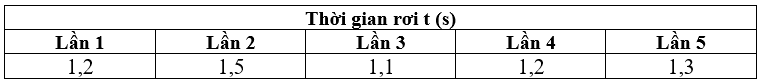
\includegraphics[scale=0.7]{figs/G10Y25B2-8}
\end{center}

\begin{ex} 
	Tính giá trị trung bình của thời gian rơi.
	\shortans[oly]{1,26}
	\loigiai{
		\begin{center}
			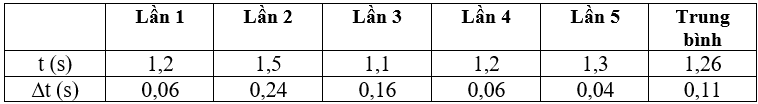
\includegraphics[scale=0.7]{figs/G10Y25B2-9}
		\end{center}
		Giá trị trung bình của thời gian rơi là: 1,26 s.
	}
\end{ex}

\begin{ex}
	Tìm sai số tuyệt đối trung bình (\textit {Kết quả làm tròn đến chữ số phần trăm}).
	\shortans[oly]{0,11}
	\loigiai{
		Sai số tuyệt đối trung bình là: 0,11 s.
	}
\end{ex}

\Closesolutionfile{ans}
\subsection{TỰ LUẬN}
\setcounter{ex}{0}
\Opensolutionfile{ans}[ans/G10Y25B2-TL]
\begin{ex}
	Một viên bị hình cầu có bán kính $r$ đang chuyển động với tốc độ $v$ trong dầu. Viên bị chịu tác dụng của lực cản có độ lớn được cho bởi biểu thức $F=c\cdot r\cdot v$, trong đó $c$ là một hằng số. Xác định đơn vị của $c$ theo đơn vị của lực, chiều dài và thời gian trong hệ SI.
	\loigiai{
		Từ công thức trên đề bài $\Rightarrow c=\dfrac{F}{r\cdot v}$\\
		Đơn vị của $c$ là: $\si{\newton\cdot\meter^{-2}\cdot\second}$.
	}
\end{ex}

\begin{ex}
	Trình bày ý nghĩa của việc sử dụng hệ đơn vị đo lường quốc tế SI trong khoa học và đời sống. Liệt kê đầy đủ 7 đơn vị cơ bản của hệ SI kèm kí hiệu và đại lượng tương ứng?
	\loigiai{
		\begin{enumerate}[label=\alph*)]
			\item \textbf{Ý nghĩa:}\\
			– Tạo sự thống nhất toàn cầu, tránh nhầm lẫn khi trao đổi dữ liệu khoa học và kĩ thuật.\\
			– Giúp chuẩn hoá thí nghiệm, thiết kế, chế tạo, kiểm định thiết bị.\\
			– Thuận tiện quy đổi giữa các ngành khoa học khác nhau.
			\item \textbf{7 đơn vị cơ bản của hệ SI:}\\[-0.7em]
			\begin{center}
				\begin{tabular}{|c|c|c|}
					\hline
					Đại lượng & Đơn vị & Kí hiệu \\ \hline
					Chiều dài & mét & \si{\meter} \\
					Khối lượng & kilôgam & \si{\kilogram} \\
					Thời gian & giây & \si{\second} \\
					Nhiệt độ & kelvin & \si{\kelvin} \\
					Cường độ dòng điện & ampe & \si{\ampere} \\
					Cường độ sáng & candela & \si{\candela} \\
					Lượng chất & mol & \si{\mole} \\ \hline
				\end{tabular}
			\end{center}
	\end{enumerate}}
\end{ex}

\begin{ex}
	Theo quy ước, vật liệu có kích thước từ \(1\) đến \(100\;\si{\nano\meter}\) được gọi là vật liệu nano. Chiều rộng trung bình của một sợi tóc người là \(50\;\si{\micro\meter}\). Sợi tóc có được coi là vật liệu nano không? Giải thích?
	\loigiai{
		Đổi đơn vị:
		\[
		50\;\si{\micro\meter}=50\times10^{3}\;\si{\nano\meter}=5{,}0\times10^{4}\;\si{\nano\meter}
		\]
		
		Giới hạn nano: \(1\;\text{nm}\le d\le100\;\text{nm}\).\\
		Kích thước sợi tóc (\(5,0\times10^{4}\;\text{nm}\)) \(\gg100\;\text{nm}\)  \(\Rightarrow\) \textbf{sợi tóc KHÔNG phải vật liệu nano}.
	}
\end{ex}

\begin{ex}
	Thực hiện các phép đổi đơn vị sau và trình bày rõ bước làm:
	\begin{itemize}
		\item \(0{,}25\;\si{\kilo\meter^{2}}\) → \si{\meter^{2}}.
		\item \(3{,}6\times10^{5}\;\si{\centi\meter^{3}}\) → \si{\meter^{3}}.
		\item \(12\;\si{\newton\meter}\) → biểu diễn thông qua các đơn vị cơ bản. Biết \(1\;\si{\newton} = 1\;\si{\kilogram\meter\second^{-2}}\).
	\end{itemize}
	\loigiai{
		\begin{enumerate}[label=\alph*)]
			\item \(1\;\si{\kilo\meter}=10^{3}\;\si{\meter}\Rightarrow 1\;\si{\kilo\meter^{2}}=(10^{3})^{2}=10^{6}\;\si{\meter^{2}}\)\\
			\(0{,}25\;\si{\kilo\meter^{2}} = 0{,}25\times10^{6} = 2{,}5\times10^{5}\;\si{\meter^{2}}\).
			\item \(1\;\si{\centi\meter}=10^{-2}\;\si{\meter}\Rightarrow 1\;\si{\centi\meter^{3}}=(10^{-2})^{3}=10^{-6}\;\si{\meter^{3}}\)\\
			\(3{,}6\times10^{5}\;\si{\centi\meter^{3}} = 3{,}6\times10^{5}\times10^{-6}=0{,}36\;\si{\meter^{3}}\).
			\item \(1\;\si{\newton} = 1\;\si{\kilogram\meter\second^{-2}}\)\\
			\(12\;\si{\newton\meter}=12\;\si{\kilogram\meter^{2}\second^{-2}}\).
	\end{enumerate}}
\end{ex}

\begin{ex}
	Cho hằng số hấp dẫn \(G = 6{,}67\times10^{-11}\;\si{\newton\meter^{2}\per\kilogram^{2}}\).
	\begin{enumerate}[label=\alph*)]
		\item Viết đơn vị của \(G\) dưới dạng các đơn vị cơ bản SI.
		\item Xác định thứ nguyên của \(G\).
	\end{enumerate}
	\loigiai{
		\begin{enumerate}[label=\alph*)]
			\item \(1\;\si{\newton}=1\;\si{\kilogram\meter\second^{-2}}\Rightarrow\)\\
			\[
			1\;\si{\newton\meter^{2}\per\kilogram^{2}}
			= \dfrac{\si{\kilogram\meter\second^{-2}}\times\si{\meter^{2}}}{\si{\kilogram^{2}}}
			= \si{\meter^{3}\kilogram^{-1}\second^{-2}}
			\]
			\item Thứ nguyên:
			\[
			[G] = L^{3}\,M^{-1}\,T^{-2}
			\]
	\end{enumerate}}
\end{ex}

\begin{ex}
	Một học sinh làm thí nghiệm đo chiều dài của bàn học bằng thước. Sau 6 lần đo, bạn học sinh tính được:
	\begin{itemize}
		\item Giá trị trung bình chiều dài bàn là $\overline{\ell}=\SI{1202}{\milli\meter}$.
		\item Sai số trung bình là $\overline{\Delta\ell}=\SI{2}{\milli\meter}$.
	\end{itemize}
	Biết sai số dụng cụ đo là $\Delta \ell_\text{dc}=\SI{1}{\milli\meter}$.\\
	Bạn hãy trình bày kết quả phép đo của học sinh trên.
	\loigiai{
		Sai số tuyệt đối của phép đo:
		$$\Delta \ell=\overline{\Delta \ell}+\Delta\ell_\text{dc}=\SI{3}{\milli\meter}.$$
		Kết quả phép đo:
		$$\ell=\overline{\ell}\pm\Delta\ell=\xsi{1202\pm3}{\milli\meter}.$$
	}
\end{ex}

\begin{ex}
	Hình \ref{fig:3P-1} thể hiện nhiệt kế đo nhiệt độ $t_1$ $\left(\si{\degree C}\right)$ và $t_2$ $\left(\si{\degree C}\right)$ của một dung dịch trước và sau khi đun. Hãy xác định và ghi kết quả độ tăng nhiệt độ $t$ của dung dịch này.
	\begin{center}
		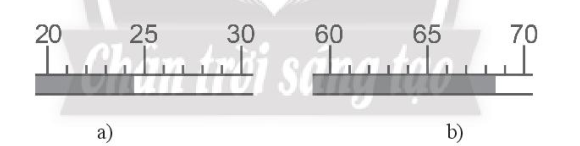
\includegraphics[scale=0.5]{figs/G10Y25B2-2}
		\captionof{figure}{Nhiệt kế: \textit{a) trước; b) sau khi đun dung dịch}}
		\label{fig:3P-1}
	\end{center}
	\loigiai{
		Lấy sai số dụng cụ $\Delta t_\text{dc}=\dfrac{\text{ĐCNN}}{2}=\SI{0.5}{\degree C}$.\\
		Nhiệt độ ban đầu:
		$$t_1=\xsi{24\pm0.5}{\degree C}$$
		Nhiệt độ lúc sau:
		$$t_2=\xsi{68\pm 0.5}{\degree C}$$
		Độ tăng nhiệt độ của dung dịch này:
		$$t=t_2-t_1=\xsi{44.0\pm1.0}{\degree C}.$$
	}
\end{ex}

\begin{ex}
	Một học sinh muốn xác định gia tốc rơi tự do $g$ bằng cách thả một quả bóng từ độ cao $h$ và dùng đồng hồ để bấm thời gian rơi $t$ của quả bóng. Sau đó, thông qua quá trình tìm hiểu, bạn sử dụng công thức $h=\dfrac{1}{2}g\cdot t^2$ để xác định $g$. Hãy nêu ít nhất 2 giải pháp giúp bạn học sinh đó giảm sai số trong quá trình thực nghiệm để thu được kết quả chính xác nhất.
	\loigiai{
		Một số giải pháp phù hợp: hạn chế sự tác động của lực cản không khí, thả rơi quả bóng ở nhiều độ cao khác nhau, sử dụng đồng hồ có độ nhạy cao, thao tác bấm đồng hồ dứt khoát.
	}
\end{ex}

\begin{ex}
	Dùng thước kẹp có ĐCNN $\SI{0.1}{mm}$ để đo 5 lần đường kính $d$ và chiều cao $h$ của một trụ thép, cho kết quả như trong bảng sau:
	\begin{center}
		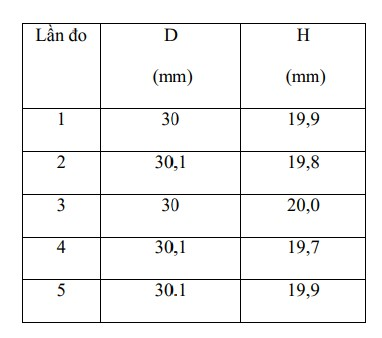
\includegraphics[scale=1]{figs/G10Y25B2-6}
	\end{center}
	Hãy cho biết kết quả phép đo $d, h$ và tính thể tích trụ thép.
	\loigiai{	
		Phép đo $d, h$ là phép đo trực tiếp, giá trị
		trung bình và sai số ngẫu nhiên tính trong
		bảng sau
		\begin{center}
			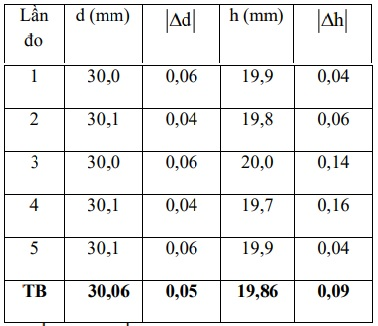
\includegraphics[scale=1]{figs/G10Y25B2-7}
		\end{center}
		Sai số dụng cụ bằng $\SI{0.1}{mm}$. Vậy:
		Sai số phép đo đường kính trụ là:
		$$\Delta d = 0.05 + 0.05 =\SI{0.10}{mm}.$$
		Sai số phép đo chiều cao trụ là:
		$$\Delta h = 0.09 + 0.05 =\SI{0.14}{mm}.$$
		Kết quả: 
		$$d = \xsi{30.06\pm0.10}{\milli\meter}.$$
		$$h = \xsi{19.86\pm0.14}{\milli\meter}.$$
		Thể tích trung bình của khối trụ:
		$$\overline{V} = \dfrac{\pi \overline{d}^2 \overline{h}}{4} =\SI{14094.42}{\cubic\milli\meter}.$$
		Sai số tỉ đối:
		$$\dfrac{\Delta V}{\overline V} = 2 \dfrac{\overline{\Delta d}}{\overline d} + \dfrac{\overline {\Delta h}}{\overline{h}} + \dfrac{\Delta \pi}{\pi} = 0.014 = \SI{1.4}{\percent}.$$
		Sai số tuyệt đối:
		$$\Delta V = \overline{V} \cdot \delta V = \SI{193.13}{\cubic\milli\meter}.$$
		Suy ra:
		$$V = \xsi{14094\pm193}{\cubic\milli\meter}.$$
	}
\end{ex}
\Closesolutionfile{ans}\newpage	% Giau (3t)
	\section{ÔN TẬP CHƯƠNG 1}
\Opensolutionfile{ans}[ans/FINAL-CHAPTER1-TL]
\setcounter{ex}{0}
\begin{ex}
	Tìm số CSCN của các số sau:
	\begin{enumerate}[label=\alph*)]
		\item $78,9\pm 0,2$;
		\item $3,788\cdot10^9$;
		\item $2,46\cdot10^6$;
		\item $0,0053$.
	\end{enumerate}
	\loigiai{
		\begin{enumerate}[label=\alph*)]
			\item 3 CSCN;
			\item 4 CSCN;
			\item 3 CSCN;
			\item 2 CSCN.
		\end{enumerate}
	}
\end{ex}

\begin{ex}
	Trong quá trình thực hành tại phòng thí nghiệm, một bạn học sinh vô tình làm vỡ nhiệt kế thuỷ ngân và làm thuỷ ngân đổ ra ngoài như Hình \ref{fig:2P-2}. Em hãy giúp bạn học sinh đó đưa ra cách xử lí thuỷ ngân đổ ra ngoài đúng cách để đảm bảo an toàn.
	\begin{center}
		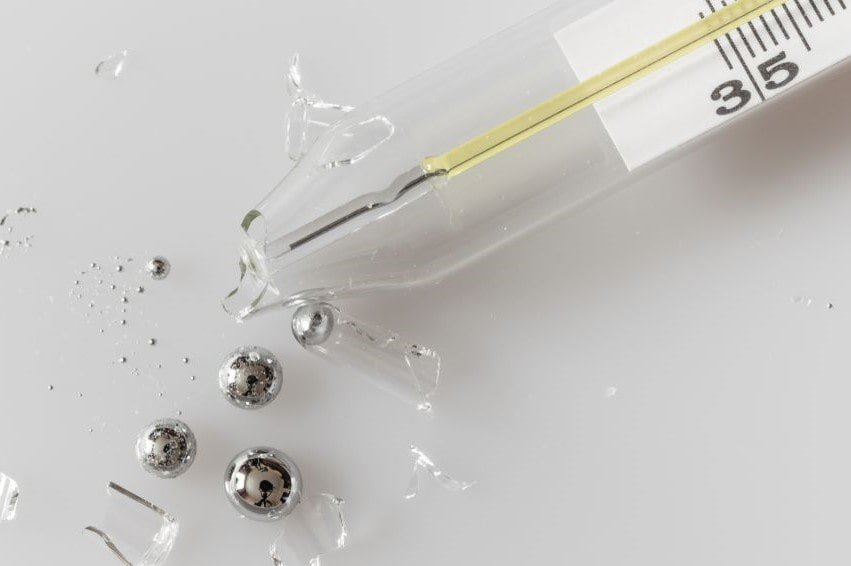
\includegraphics[width=0.3\linewidth]{figs/FINAL-CHAPTER1-2}
		\captionof{figure}{Thuỷ ngân bị đổ ra khỏi nhiệt kế}
		\label{fig:2P-2}
	\end{center}
	\loigiai{
		Cách xử lí đúng nguyên tắc an toàn: báo cho giáo viên tại phòng thí nghiệm, sơ tán các bạn học sinh ở khu vực gần đó, tắt quạt và đóng hết cửa sổ để tránh việc thuỷ ngân phát tán trong không khí. Người dọn dẹp phải sử dụng găng tay và khẩu trang để dọn sạch thuỷ ngân, tuyệt đối không được tiếp xúc với thuỷ ngân bằng tay trần.
	}
\end{ex}

\begin{ex}
	Theo em, tốc độ bay hơi của nước phụ thuộc vào những đặc điểm nào? Hãy dựa trên những hiện tượng thường thấy hằng ngày để đưa ra giả thuyết và thiết kế phương án thí nghiệm kiểm tra giải thuyết của mình.
	\loigiai{
		Nhiệt độ của nước, gió trên mặt thoáng của nước và diện tích mặt thoáng của nước.
	}
\end{ex}

\begin{ex}
	Hai người cùng đo chiều dài của cánh cửa sổ, kết quả thu được như sau:
	\begin{itemize}
		\item Người thứ nhất: $d=\xsi{120\pm1}{\centi\meter}$;
		\item Người thứ hai: $d=\xsi{120\pm 2}{\centi\meter}$;
	\end{itemize}
	Trong hai người, ai là người đo chính xác hơn? Vì sao?
	\loigiai{
		Người 1 đo chính xác hơn vì với cùng một giá trị trung bình nhưng sai số tuyệt đối trong phép đo của người 1 bé hơn sai số tuyệt đối trong phép đo của người 2.\\
		Hoặc có thể tính sai số tỉ đối $\delta_1=\SI{0.83}{\percent}$ và $\delta_2=\SI{1.67}{\percent}$. Vì $\delta_1<\delta_2$ nên người 1 đo chính xác hơn.	
	}
\end{ex}

\begin{ex}
	Một tấm bìa hình chữ nhật có chiều dài $\xsi{\left(21.3\pm0.2\right)}{\centi\meter}$ và chiều rộng $\xsi{\left(9.8\pm0.1\right)}{\centi\meter}$. Tính diện tích của tấm bìa.
	\loigiai{
		$$S=\xsi{\left(21.3\pm0.2\right)\times\left(9.8\pm0.1\right)}{\square\centi\meter}=\xsi{\left(21.3\times 9.8 \pm 21.3\times 0.1 \pm 9.8\times 0.2 \pm 0.1\times 0.2\right)}{\square\centi\meter}= \xsi{\left(209\pm4\right)}{\square\centi\meter}.$$
		Hoặc
		$$\overline{S}=\overline{d}\times \overline{r}=\xsi{21.3\times 9.8}{\square\centi\meter}=\SI{208.8}{\square\centi\meter}$$
		$$\Delta S=\left(\dfrac{\Delta d}{\overline{d}}+\dfrac{\Delta r}{\overline{r}}\right)\times \overline{S}=\SI{4.1}{\square\centi\meter}$$
		Vậy kết quả đo diện tích của tấm bìa $S=\xsi{\left(209\pm4\right)}{\square\centi\meter}.$
	}
\end{ex}

\begin{ex}
	Một học sinh đo cường độ dòng điện đi qua các đèn $\text{Đ}_1$ và $\text{Đ}_2$ như Hình \ref{fig:0001-1} được các giá trị lần lượt là 
	\begin{center}
		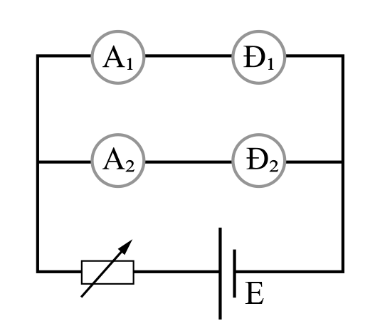
\includegraphics[width=0.3\linewidth]{figs/FINAL-CHAPTER1-1}
		\captionof{figure}{}
		\label{fig:0001-1}
	\end{center}
	$$I_1=\xsi{\left(2.0\pm0.1\right)}{\ampere}$$
	$$I_2=\xsi{\left(1.5\pm0.2\right)}{\ampere}$$
	Cường độ dòng điện mạch chính được cho bởi
	$$I=I_1+I_2$$
	Tính giá trị và viết kết quả của $I$.
	\loigiai{
		$$I=\xsi{\left(3.5\pm0.3\right)}{\ampere}.$$
	}
\end{ex}

\begin{ex}
	Một nhóm học sinh đo được hiệu điện thế giữa hai đầu một điện trở là $\xsi{\left(10.0\pm0.3\right)}{\volt}$ và cường độ dòng điện qua điện trở là $\xsi{\left(1.3\pm0.2\right)}{\ampere}$. Viết kết quả tính giá trị của điện trở.
	\loigiai{
		Ta có: $R=\dfrac{U}{I}$\\
		Giá trị trung bình $$\overline{R}=\dfrac{\overline{U}}{\overline{I}}=\SI{7.7}{\ohm}$$
		Sai số tuyệt đối:
		$$\Delta R =\left(\dfrac{\Delta U}{\overline{U}}+\dfrac{\Delta I}{\overline{I}}\right)\cdot\overline{R}=\SI{1.4}{\ohm}$$
		Vậy kết quả tính giá trị điện trở $R=\xsi{\left(7.7\pm1.4\right)}{\ohm}.$
	}
\end{ex}

\begin{ex}
	Cho bảng số liệu thể hiện kết quả đo khối lượng của một túi trái cây bằng cân đồng hồ. Em hãy xác định sai số tuyệt đối ứng với từng lần đo, sai số tuyệt đối và sai số tương đối của phép đo. Biết sai số dụng cụ là $\SI{0.1}{\kilogram}$.
	\begin{center}
		\begin{tabular}{|c|c|c|}
			\hline
			\thead{Lần đo} & \thead{$\xsi{m}{\left(\kilogram\right)}$} & \thead{$\xsi{\Delta m}{\left(\kilogram\right)}$}\\
			\hline
			1& $4,2$ & \dots\\
			\hline
			2& $4,4$ & \dots\\
			\hline
			3& $4,4$ & \dots\\
			\hline
			4& $4,2$ & \dots\\
			\hline
		\end{tabular}
	\end{center}
	\loigiai{
		\begin{center}
			\begin{tabular}{|c|c|c|}
				\hline
				\thead{Lần đo} & \thead{$\xsi{m}{\left(\kilogram\right)}$} & \thead{$\xsi{\Delta m}{\left(\kilogram\right)}$}\\
				\hline
				1& $4,2$ & $0,1$\\
				\hline
				2& $4,4$ & $0,1$\\
				\hline
				3& $4,4$ & $0,1$\\
				\hline
				4& $4,2$ & $0,1$\\
				\hline
				Trung bình &$4,3$ & $0,1$\\
				\hline
			\end{tabular}
		\end{center}
		Sai số tuyệt đối: $\Delta m=\overline{\Delta m}+\Delta m_\text{dc}=\SI{0.2}{\kilogram}$.\\
		Sai số tương đối: $\delta m=\dfrac{\Delta m}{\overline{m}}=\SI{4.65}{\percent}$.\\
		Kết quả đo: $m=\xsi{4.3\pm0.2}{\kilogram}$.
	}
\end{ex}

\begin{ex}
	Giá trị đo gia tốc rơi tự do $g$ có thể được xác định bằng cách đo chu kì dao động của con lắc đơn có chiều dài $\ell$. Mối quan hệ giữa $g, T$ và $\ell$ là 
	$$g=4\pi^2\left(\dfrac{\ell}{T^2}\right)$$
	Trong một thí nghiệm, đo được:
	$$\ell=\xsi{\left(0.55\pm0.02\right)}{\meter}; T=\xsi{\left(1.50\pm0.02\right)}{\second}$$
	Tìm giá trị và viết kết quả của $g$.
	\loigiai{
		Giá trị trung bình:
		$$\overline{g}=4\pi^2\cdot\dfrac{\overline{\ell}}{\overline{T}^2}$$
		Sai số tuyệt đối
		$$\Delta g=\left(\dfrac{\Delta \ell}{\overline{\ell}}+2\cdot\dfrac{\Delta T}{\overline{T}}\right)\cdot\overline{g}=\SI{0.6}{\meter\per\square\second}$$
		Kết quả đo:
		$$g=\xsi{\left(9.7\pm0.6\right)}{\meter\per\square\second}.$$
	}
\end{ex}

\begin{ex}
	Một học sinh dùng thước có ĐCNN là $\SI{1}{\milli\meter}$ và một đồng hồ đo thời gian có ĐCNN $\SI{0.01}{\second}$ để đo 5 lần thời gian chuyển động của một chiếc xe đồ chơi chạy bằng pin từ điểm $A$ đến điểm $B$. Kết quả đo được cho ở bảng sau
	\begin{center}
		\begin{tabular}{|c|c|c|c|c|}
			\hline
			\thead{Lần đo}& \thead{$\xsi{s}{\left(\meter\right)}$} &\thead{$\xsi{\Delta s}{\left(\meter\right)}$} & \thead{$\xsi{t}{\left(\second\right)}$} & \thead{$\xsi{\Delta t}{\left(\second\right)}$}\\
			\hline
			1 & $0,546$ & \dots & $2,47$ & \dots\\
			\hline
			2 & $0,554$ & \dots & $2,51$ & \dots\\
			\hline
			3 & $0,549$ & \dots & $2,42$ & \dots\\
			\hline
			4 & $0,560$ & \dots & $2,52$ & \dots\\
			\hline
			5 & $0,551$ & \dots & $2,48$ & \dots\\
			\hline
		\end{tabular}
	\end{center}
	\begin{enumerate}[label=\alph*)]
		\item Nêu nguyên nhân gây ra sự sai khác giữa các lần đo?
		\item Tính sai số tuyệt đối và sai số tỉ đối của phép đo $s$, $t$.
		\item Biểu diễn kết quả đo $s$ và $t$.
		\item Tính sai sối tỉ đối $\delta v$ sai số tuyệt đối $\Delta v$. Biểu diễn kết quả tính $v$.
	\end{enumerate}
	\loigiai{
		\begin{enumerate}[label=\alph*)]
			\item Nguyên nhân gây ra sai khác giữa các lần đo: Do cấu tạo của dụng cụ thí nghiệm, thao tác khi đo chưa chuẩn xác.
			\item $\Delta s=\SI{0.0055}{\meter}$; $\Delta t=\SI{0.035}{\second}$.
			\item $s=\xsi{0.5520\pm0.0055}{\meter}$; $t=\xsi{2.480\pm0.035}{\second}$.
			\item $\delta v=\SI{2.41}{\percent}$; $\Delta v=\SI{0.0054}{\meter\per\second}$.\\
			Kết quả tính: $v=\xsi{0.2226\pm0.0054}{\meter\per\second}$.
		\end{enumerate}
	}
\end{ex}
\Closesolutionfile{ans}\newpage	% Uyên (2t)
%%% CHƯƠNG 2: MÔ TẢ CHUYỂN ĐỘNG
	\chapter{MÔ TẢ CHUYỂN ĐỘNG}
\section{CHUYỂN ĐỘNG THẲNG}
\subsection{LÝ THUYẾT TRỌNG TÂM}
\begin{tomtat}
	\subsubsection{Chuyển động cơ. Chất điểm}
	\paragraph{Chuyển động cơ}
	\begin{dn}
		Chuyển động cơ của một vật (gọi tắt là chuyển động) là sự thay đổi vị trí của vật đó so với các vật khác theo thời gian.
	\end{dn}
	\paragraph{Chất điểm}
	\begin{dn}
		Một vật chuyển động được coi là một chất điểm nếu kích thước của nó rất nhỏ so với độ dài đường đi (hoặc so với những khoảng cách mà ta đề cập đến).
	\end{dn}
	
	\textbf{\textit{Ví dụ:}} trong chuyển động của ô tô từ thành phố Hồ Chí Minh đến Hà Nội thì ô tô được xem là chất điểm.
	\paragraph{Quỹ đạo}
	\begin{dn}
		Tập hợp tất cả các vị trí của một chất điểm chuyển động tạo ra một đường trong không gian, đường đó gọi là quỹ đạo của chuyển động.
	\end{dn}
%	\subsubsection{Cách xác định vị trí của vật trong không gian}
%	\paragraph{Vật làm mốc và thước đo}
%	Nếu đã biết đường đi (quỹ đạo) của vật, ta cần chọn một vật làm mốc và một chiều dương trên đường đi, và dùng thước đo chiều dài đoạn đường từ vật làm mốc đến vật là có thể xác định được chính xác vị trí của vật.
%	\begin{center}
%		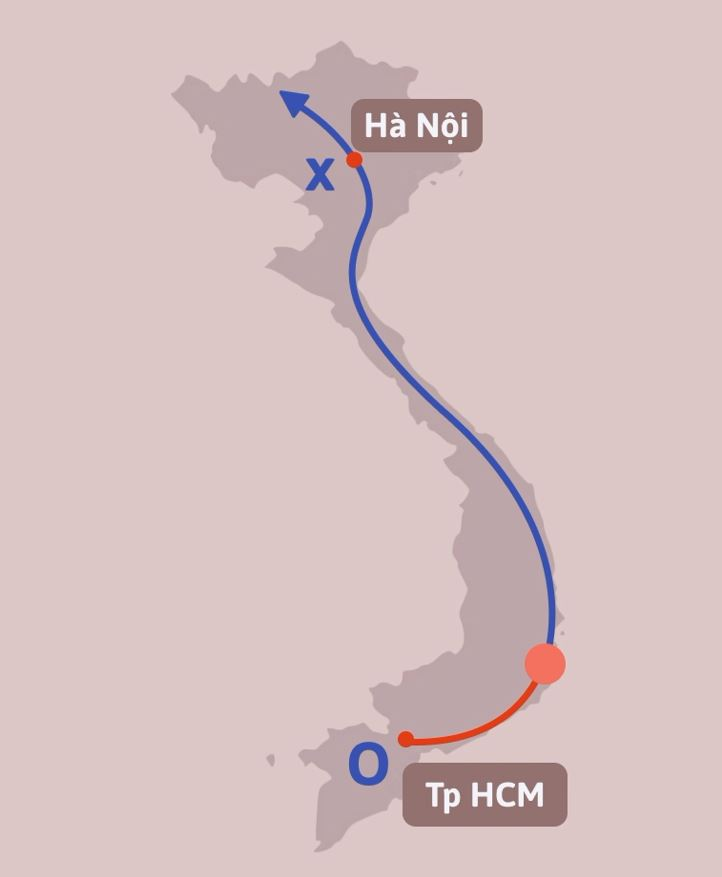
\includegraphics[scale=0.3]{figs/G10Y25B3-1}
%	\end{center}
%	\paragraph{Hệ tọa độ}
%	Muốn xác định vị trí của một điểm trên một mặt phẳng ta cần có hệ tọa độ với hai trục $Ox$ và $Oy$ vuông góc nhau, hình chiếu vuông góc của điểm xuống hai trục tọa độ đó chính là tọa độ của điểm đó.
%	\begin{center}
%		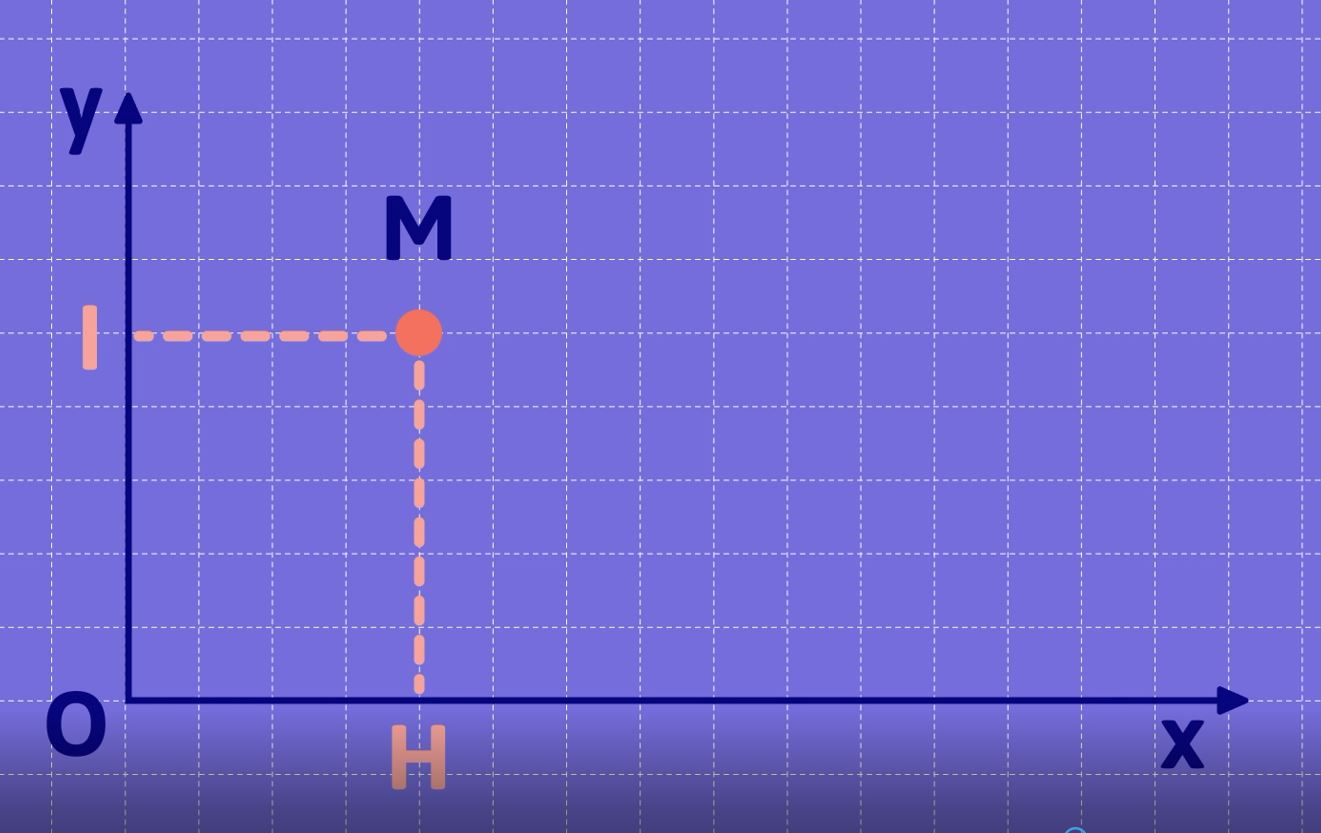
\includegraphics[scale=0.4]{figs/G10Y25B3-2}
%	\end{center}
%	\subsubsection{Cách xác định thời gian trong chuyển động}
%	\subsubsection{Mốc thời gian và đồng hồ}
%	Để mô tả chuyển động của một vật ta phải biết tọa độ của vật đó ở những thời điểm khác nhau. Muốn thế, ta phải chỉ rõ mốc thời gian và đo khoảng thời gian trôi đi kể từ mốc thời gian bằng một đồng hồ.
%	\subsubsection{Thời điểm và thời gian}
%	Nếu lấy mốc thời gian là thời điểm vật bắt đầu chuyển động (thời điểm 0) thì số chỉ của thời điểm sẽ trùng với số đo khoảng thời gian đã trôi qua kể từ mốc thời gian.
%	\subsection{Hệ quy chiếu}
%	Một hệ quy chiếu gồm:
%	\begin{itemize}
%		\item mốc tọa độ và một hệ tọa độ để đo vị trí;
%		\item mốc thời gian và một đồng hồ để xác định thời điểm.
%	\end{itemize}
	\subsubsection{Độ dịch chuyển và quãng đường đi được}
	\paragraph{Độ dịch chuyển}
	\begin{dn}
		Độ dịch chuyển được xác định bằng độ biến thiên toạ độ của vật
		$$d=x_2-x_1=\Delta x$$
	\end{dn}
	\begin{center}
		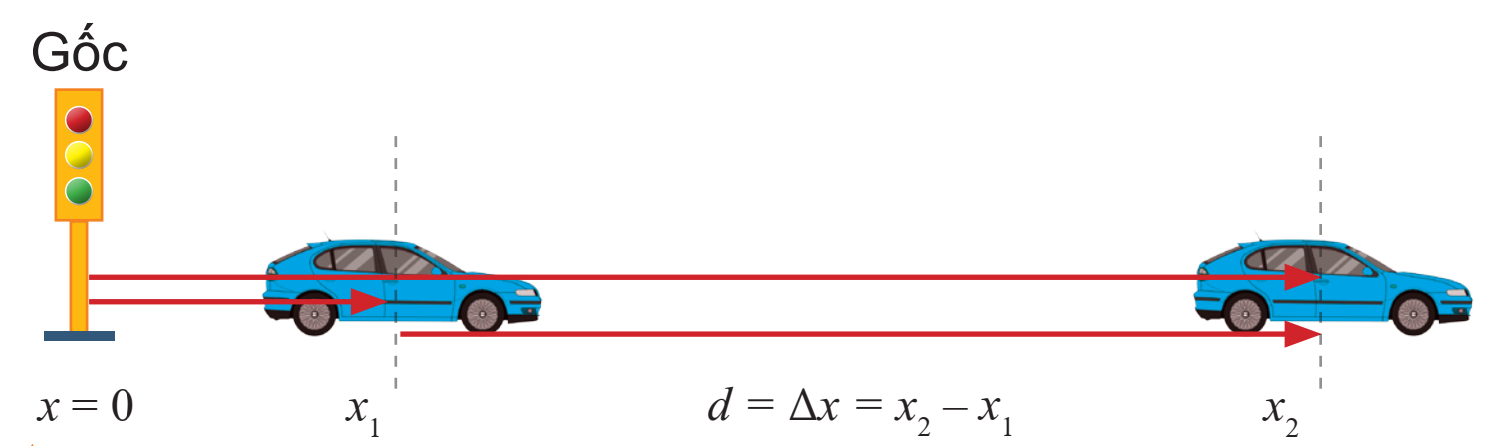
\includegraphics[scale=0.5]{figs/G10Y25B3-3}
		\captionof{figure}{Ví dụ thực tế về độ dịch chuyển của vật trên đường thẳng}
	\end{center}
	\begin{tc}
		Độ dịch chuyển có các đặc điểm sau:
		\begin{itemize}
			\item độ dịch chuyển là một đại lượng vector $\left(\vec{d}\right)$ có gốc tại vị trí ban đầu, hướng từ vị trí đầu đến vị trí cuối, độ lớn bằng khoảng cách giữa vị trí đầu và vị trí cuối.
			\item độ dịch chuyển là một đại lượng có thể nhận giá trị dương, âm hoặc bằng không. 
		\end{itemize}
	\end{tc}
	\paragraph{So sánh độ dịch chuyển và quãng đường đi được}
	\begin{longtable}{|m{20em}|m{20em}|}
		\hline
		\thead{Độ dịch chuyển $\left(\vec{d}\right)$} & \thead{Quãng đường $\left(s\right)$}\\
		\hline
		Là đại lượng vector. & Là đại lượng vô hướng.\\
		\hline
		Cho biết sự thay đổi vị trí của một vật (về hướng và độ dời). & Cho biết độ dài mà vật đi được.\\
		\hline
		Có thể nhận giá trị dương, âm hoặc bằng 0. & Có giá trị không âm.\\
		\hline
	\end{longtable}
	\begin{luuy}
		Khi vật chuyển động theo một hướng (chuyển động thẳng và không đổi chiều) thì độ lớn của độ dịch chuyển và quãng đường đi được bằng nhau $(d=s)$.
	\end{luuy}
	\subsubsection{Tốc độ trung bình - Vận tốc trung bình}
	\paragraph{Tốc độ trung bình}
	\begin{dn}
		Tốc độ trung bình $\overline{v}_{\text{tb}}$ là đại lượng đặc trưng cho mức độ nhanh hay chậm của chuyển động; được đo bằng thương số giữa quãng đường đi được $s$ và khoảng thời gian $t$ để đi hết quãng đường đó:
		\begin{equation}
			\overline{v}_{\text{tb}}=\dfrac{s}{t}.
		\end{equation}
	\end{dn}
	Trong hệ SI, đơn vị của tốc độ trung bình là \si{\meter/\second}. Các đơn vị khác cũng thường được sử dụng là \si{\kilo\meter/\hour}, \si{\centi\meter/\second}, \dots
	\begin{noidung}{Tốc độ tức thời}
		Tốc độ trung bình tính trong khoảng thời gian rất nhỏ là tốc độ tức thời (kí hiệu $v$) diễn tả sự nhanh, chậm của chuyển động tại thời điểm đó.
	\end{noidung}
	\begin{luuy}
		\begin{itemize}
			\item Khi một vật chuyển động với tốc độ tức thời không đổi, ta nói chuyển động của vật là chuyển động đều. Ngược lại, ta nói chuyển động của vật là không đều.
			\item Trên thực tế, tốc độ tức thời được hiển thị bởi tốc kế trên nhiều phương tiện giao thông.
		\end{itemize}
	\end{luuy}
	\paragraph{Vận tốc trung bình}
	\begin{dn}
		Vận tốc trung bình là đại lượng vectơ được xác định bằng thương số giữa độ dịch chuyển của vật và thời gian để vật thực hiện độ dịch chuyển đó
		$$v_\text{tb}=\dfrac{\vec{d}}{\Delta t}=\dfrac{\Delta \vec{x}}{\Delta t}.$$
	\end{dn}
	\begin{luuy}
		Tốc độ trung bình chỉ bằng độ lớn của vận tốc trung bình khi vật chuyển động thẳng không đổi chiều.
	\end{luuy}
	\subsubsection{Phương trình chuyển động thẳng đều}
	Xét một chất điểm chuyển động thẳng đều trên đường thẳng O$x$ với tốc độ $v$. Ở thời điểm ban đầu ($t_0=0$), vật ở vị trí A cách gốc O một đoạn $x_0$. Vào thời điểm $t$, vật ở vị trí M cách gốc O một đoạn $x$.  
	\begin{center}
		\begin{tikzpicture}
			\coordinate (O) at (0,0);
			\coordinate (A) at (2,0);
			\coordinate (M) at (5,0);
			\coordinate (x) at (8,0);
			\coordinate (O1) at ($(O)-(0,1cm)$);
			\coordinate (A1) at ($(A)-(0,1cm)$);
			\draw[->,thick] (O) -- (x);
			\foreach \i in {O,A}{
				\filldraw[black] (\i) circle (0.5mm);
			}
			\node[label=90:O] at (O){};	
			\node[label=90:A] at (A){};
			\node[label=90:M] at (M){};	
			\node[label=90:x] at (x){};	
			\draw[<->] (O1) -- (A1);
			\node [fill=white] (F1) at ($(O1)!0.5!(A1)$) {$x_0$};
			\coordinate (M1) at ($(M)-(0,1cm)$);
			\draw[<->] (A1) -- (M1);
			\node [fill=white] (F2) at ($(A1)!0.5!(M1)$) {$s$};
			\coordinate (O2) at ($(O)-(0,1.5cm)$);
			\coordinate (M2) at ($(M)-(0,1.5cm)$);
			\draw[<->] (O2) -- (M2);
			\node [fill=white] (F3) at ($(O2)!0.5!(M2)$) {$x$};
			\draw[dashed] (O) -- (O2);
			\draw[dashed] (A) -- (A1);
			\draw[dashed] (M) -- (M2);
			\filldraw[blue] (M) circle (0.5mm);
			%		\node[above of=O]()
		\end{tikzpicture}
	\end{center}
	
	Tọa độ của chất điểm sau thời gian chuyển động $t$ là:
	\begin{equation}
		x=x_0+s=x_0+vt.
	\end{equation}
	Phương trình dùng để xác định tọa độ của M theo thời gian được gọi là phương trình chuyển động của chất điểm M. Trong trường hợp này, M chuyển động thẳng đều nên phương trình này gọi là phương trình chuyển động thẳng đều của điểm M. 
	\subsubsection{Đồ thị độ dịch chuyển - Thời gian}
	\paragraph{Đồ thị độ dịch chuyển - thời gian}
	Đồ thị độ dịch chuyển - thời gian của hai vật A và B được mô tả như hình \ref{fig:5.1}
	\begin{center}
		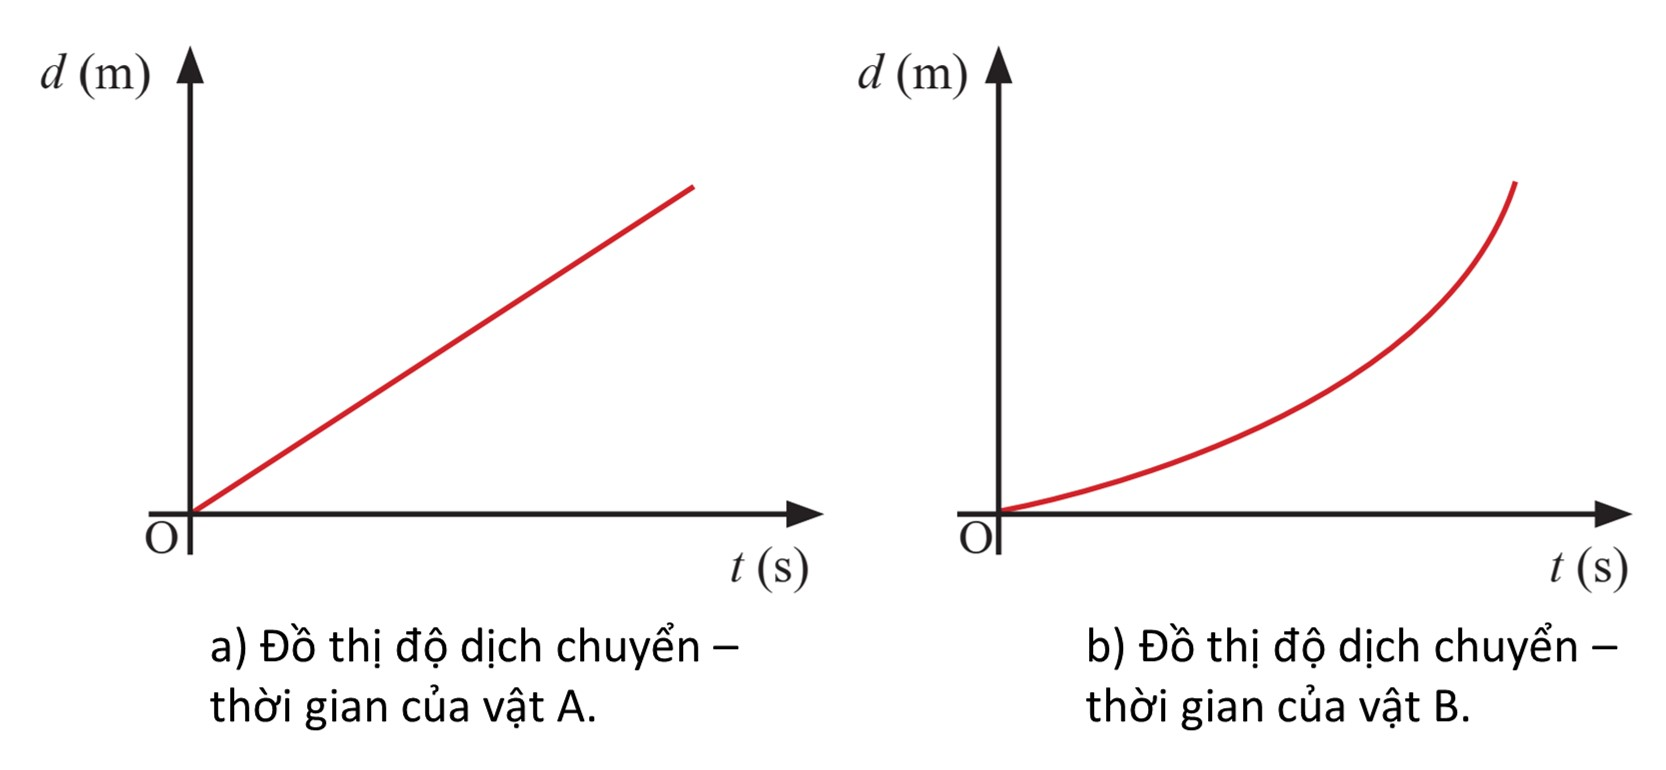
\includegraphics[scale=0.5]{figs/G10Y25B3-18}
		\captionof{figure}{}
		\label{fig:5.1}
	\end{center}
	Từ các đồ thị $\left(d-t\right)$, ta có nhận xét:
	\begin{enumerate}[label=\alph*)]
		\item Đồ thị $\left(d-t\right)$ mô tả chuyển động của vật $A$ là đường thẳng đi qua gốc toạ độ. Chuyển động của vật $A$ là chuyển động thẳng đều.
		\item Đồ thị $\left(d-t\right)$ mô tả chuyển động của vật $B$ là đường cong qua gốc toạ độ. Độ dịch chuyển của vật B trong những khoảng thời gian bằng nhau tăng lên nên chuyển động của vật B là chuyển động thẳng nhanh dần.
	\end{enumerate}
	\paragraph{Xác định vận tốc từ độ dốc của đồ thị độ dịch chuyển - thời gian}
	\begin{tc}
		Vận tốc tức thời của vật tại một thời điểm được xác định bởi độ dốc của tiếp tuyến với đồ thị $\left(d-t\right)$ tại thời điểm đang xét.\\
		Tốc độ tức thời tại một thời điểm chính là độ lớn của độ dốc tiếp tuyến của đồ thị $\left(d-t\right)$ tại điểm đó.
	\end{tc}
	\begin{center}
		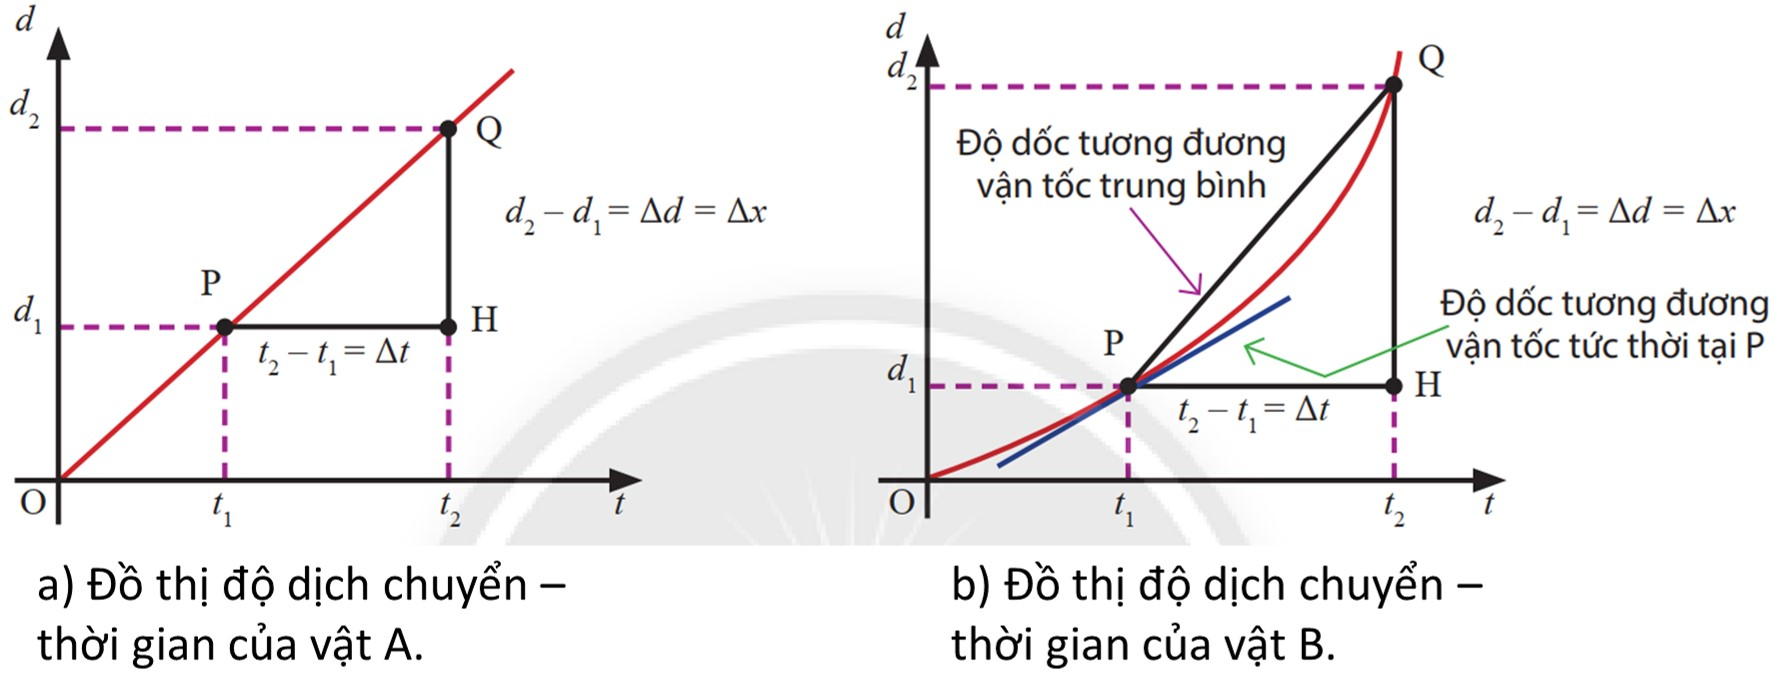
\includegraphics[scale=0.5]{figs/G10Y25B3-19}
		\captionof{figure}{}
		\label{fig:5.2}
	\end{center}
	
\end{tomtat}
\subsection{VÍ DỤ MINH HỌA}
\begin{dang}{Thực hiện xác định thời điểm và thời gian (mốc thời gian và đồng hồ)}
\end{dang}
\begin{vd}
	Giờ Berlin chậm hơn giờ Hà Nội 5 giờ. Trận bóng đá diễn ra tại Beclin lúc 19h00 ngày 2-9-2021. Khi đó theo giờ Hà Nội là
	\choice
	{14h00 ngày 3-9-2021}
	{\True 0h00 ngày 3-9-2021}
	{0h00 ngày 2-9-2021}
	{14h00 ngày 2-9-2021}
	\loigiai{	
		Giờ Berlin chậm hơn giờ Hà Nội 5 giờ, nghĩa là
		$$t_{\text{B}}+\SI{5}{\hour}=t_{\text{HN}}.$$
		Trận bóng đá diễn ra tại Berlin lúc 19h00 ngày 2-9-2021. Thời điểm đó theo giờ Hà Nội là:
		$$t_{\text{HN}}=t_{\text{B}}+\SI{5}{\hour}=19\text{h}00 + 5\text{h} = 24\text{h}00$$
		Một ngày chỉ có 24 giờ nên thời điểm trên đã bước sang ngày hôm sau. Do đó, trận bóng trên diễn ra vào lúc 0h00 ngày 3-9-2021 giờ Hà Nội. 	
	}
\end{vd}

\begin{vd}
	Theo lịch trình tại bến xe ở Hà Nội thì ô tô chở khách trên tuyến Hà Nội - Hải Phòng chạy từ Hà Nội lúc 6 giờ sáng, đi qua Hải Dương lúc 7 giờ 15 phút sáng và tới Hải Phòng lúc 8 giờ 50 phút sáng cùng ngày. Hà Nội cách Hải Dương 60 km và cách Hải Phòng $\SI{105}{km}$. Xe ô tô chạy liên tục không nghỉ dọc đường, chỉ dừng lại 10 phút tại bến xe Hải Dương để đón, trả khách. Tính khoảng thời gian chuyển động và quãng đường đi được của các hành khách sau:
	\begin{enumerate}[label=\alph*)]
		\item Hành khách lên xe tại Hà Nội đi Hải Phòng.
		\item Hành khách lên xe tại Hải Dương đi Hải Phòng.
	\end{enumerate}
	\loigiai{
		\begin{enumerate}[label=\alph*)]
			\item Đối với hành khách lên xe tại Hà Nội đi Hải Phòng, chọn bến xe Hà Nội làm mốc và thời điểm ô tô bắt đầu xuất phát là mốc thời gian.
			
			Khoảng thời gian chuyển động là:	
			\begin{center}
				(8 giờ 50 phút - 6 giờ) - 10 phút = 2 giờ 40 phút.
			\end{center}
			Quãng đường đi được đúng bằng độ dài của đoạn đường Hà Nội - Hải Phòng là $\SI{105}{km}$.
			\item Đối với hành khách lên xe tại Hải Dương đi Hải Phòng, chọn bến xe Hải Dương làm mốc và thời điểm ô tô bắt đầu xuất phát là mốc thời gian.
			
			Khoảng thời gian chuyển động là:
			\begin{center}
				8 giờ 50 phút - (7 giờ 15 phút + 10 phút) = 1 giờ 25 phút.
			\end{center}
			Quãng đường đi được là:
			$$\SI{105}{km}-\SI{60}{km}=\SI{45}{km}.$$
		\end{enumerate}
	}
\end{vd}

\begin{dang}{So sánh được quãng đường đi được và độ dịch chuyển.}
	\begin{center}
		\begin{tabular}{|M{8cm}|M{8cm}|}
			\hline
			\thead{Độ dịch chuyển $\left(\vec{d}\right)$} & \thead{Quãng đường $\left(s\right)$}\\
			\hline
			Đại lượng vector \textit{(gốc tại vị trí ban đầu, hướng từ vị trí đầu đến vị trí cuối)}. & Đại lượng vô hướng.\\
			\hline
			Xác định bằng độ biến thiên tọa độ: $d=x_2-x_1=\Delta x$. & Xác định bằng tổng chiều dài đoạn đường đi.\\
			\hline
			Có thể nhận giá trị dương, âm hoặc bằng 0. & Nhận giá trị không âm.\\
			\hline
			
		\end{tabular}
	\end{center}
\end{dang}
\begin{vd}
	Xét quãng đường $AB$ dài $\SI{1000}{\meter}$ với $A$ là vị trí nhà của em và $B$ là vị trí của bưu điện. Tiệm tạp hóa nằm tại vị trí $C$ là trung điểm của $AB$. Nếu chọn nhà em làm gốc tọa độ và chiều dương hướng từ nhà em đến bưu điện. Hãy xác định độ dịch chuyển và quãng đường đi được của em trong các trường hợp:
	\begin{center}
		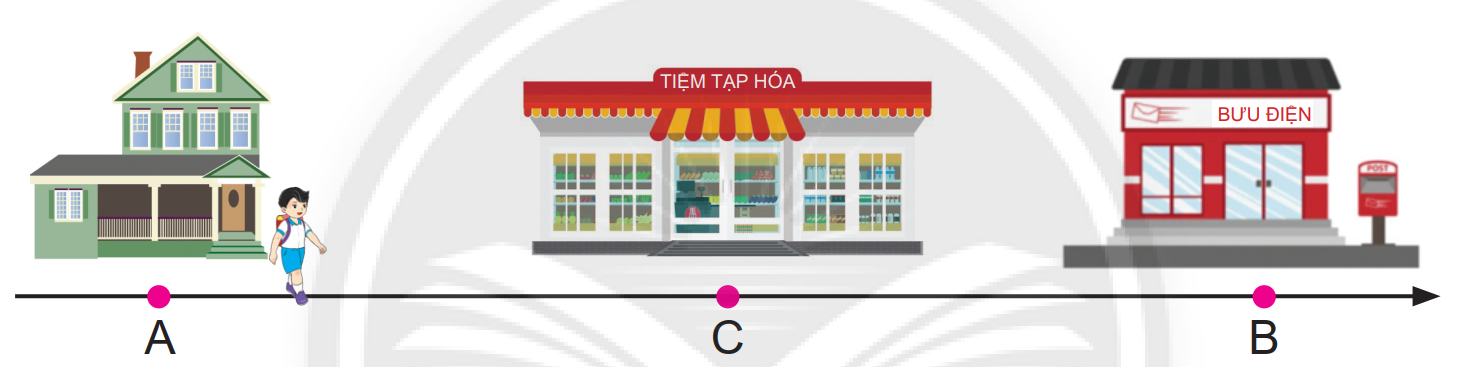
\includegraphics[width=0.6\linewidth]{figs/G10Y25B3-4}
	\end{center}
	\begin{enumerate}[label=\alph*)]
		\item Đi từ nhà đến bưu điện.
		\item Đi từ nhà đến bưu điện rồi quay lại tiệm tạp hóa.
		\item Đi từ nhà đến tiệm tạp hóa rồi quay về. 
	\end{enumerate}	
	\loigiai{
		\begin{enumerate}[label=\alph*)]
			\item Độ dịch chuyển $d=AB=x_B-x_A=\SI{1000}{\meter}-\SI{0}{\meter}=\SI{1000}{\meter}$.\\
			Quãng đường đi được $s=AB=\SI{1000}{\meter}$.
			\item Độ dịch chuyển $d=AC=x_A-x_C=\SI{500}{\meter}-\SI{0}{\meter}=\SI{500}{\meter}$.\\
			Quãng đường đi được $s=AB+BC=\SI{1500}{\meter}$.
			\item Độ dịch chuyển $d=x_A-x_A=\SI{0}{\meter}$.\\
			Quãng đường đi được $s=2AC=\SI{1000}{\meter}$.
		\end{enumerate}
	}
\end{vd}

\begin{vd}
	Một vận động viên chạy từ cổng Dinh Thống Nhất (A) đến Thảo Cầm Viên (D) theo hai quỹ đạo khác nhau. Hãy xác định độ dịch chuyển và quãng đường chạy được của người vận động viên trong 2 trường hợp trên.
	\begin{center}
		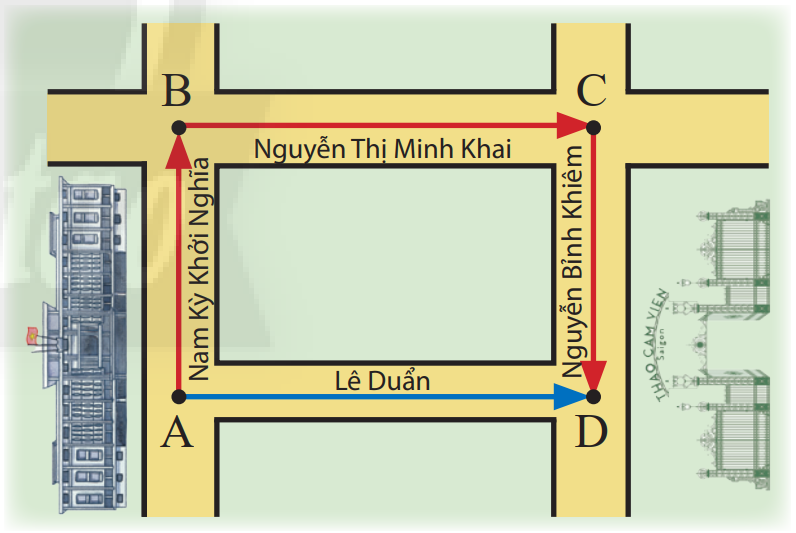
\includegraphics[width=0.5\linewidth]{figs/G10Y25B3-5}
	\end{center}
	\loigiai{
		\textbf{Trường hợp 1:} Nếu vận động viên chạy theo đường Lê Duẩn thì\\
		Độ dời $\vec{d}=\overrightarrow{AD}$, về độ lớn thì $d=AD$.\\
		Quãng đường $s=AD$.\\
		\textbf{Trường hợp 2:} Nếu vận động viên chạy theo đường Nam Kì Khởi Nghĩa qua đường Nguyễn Thị Minh Khai rồi mới đến Thảo Cầm Viên ở đường Nguyễn Bỉnh Khiêm thì\\
		Độ dời $\vec{d}=\overrightarrow{AD}$, về độ lớn thì $d=AD$.\\
		Quãng đường $s=AB+BC+CD$.
	}
\end{vd}
\begin{dang}{Mối liên hệ giữa quãng đường đi và tốc độ trung bình}
$$\overline{v}_{\mathrm{tb}}=\dfrac{s}{t}.$$
\end{dang}
\begin{vd}
	Một ô tô đi trên con đường bằng phẳng với tốc độ trung bình $v = \SI{60}{km/h}$, trong thời gian 5 phút, sau đó lên dốc 3 phút với tốc độ trung bình $v = \SI{40}{km/h}$. Tính quãng đường ô tô đã đi trong cả giai đoạn.
	\loigiai{
		Quãng đường ô tô đi được trên đoạn đường phẳng
		$$s_1 =v_1t_1 =\SI{60}{\kilo\meter/\hour}\cdot\SI{5}{\minute}=\dfrac{\SI{60}{\kilo\meter}}{\SI{1}{\hour}}\cdot\SI{5}{\minute}=\dfrac{\SI{60}{\kilo\meter}}{\SI{60}{\minute}}\cdot\SI{5}{\minute}=\SI{5}{km}.$$
		
		Quãng đường ô tô lên dốc
		$$s_2 = v_2t_2=\SI{40}{\kilo\meter/\hour}\cdot\SI{3}{\minute}=\dfrac{\SI{40}{\kilo\meter}}{\SI{1}{\hour}}\cdot\SI{3}{\minute}=\dfrac{\SI{40}{\kilo\meter}}{\SI{60}{\minute}}\cdot\SI{3}{\minute} = \SI{2}{km}.$$
		
		Quãng đường ô tô đã đi trong cả giai đoạn
		$$s = s_1+s_2 = \SI{7}{km}.$$
	}
\end{vd}

\begin{vd}
	Hai xe cùng chuyển động đều trên đường thẳng. Nếu chúng đi ngược chiều thì cứ 30 phút khoảng cách của chúng giảm $\SI{40}{km}$. Nếu chúng đi cùng chiều thì cứ sau 20 phút khoảng cách giữa chúng giảm $\SI{8}{km}$. Tính tốc độ của mỗi xe.
	\loigiai{
		Nếu đi ngược chiều thì 
		\begin{eqnarray}
			s_1+s_2 &=&(v_1+v_2)t_1 =\SI{40}{\kilo\meter}\nonumber\\
			\Rightarrow\qquad v_1+v_2&=&\dfrac{\SI{40}{\kilo\meter}}{\SI{0.5}{\hour}}=\SI{80}{\kilo\meter/\hour}\label{eq:tongv}
		\end{eqnarray}
		Nếu đi cùng chiều thì	
		\begin{eqnarray}
			s'_1-s'_2 &=&(v_1-v_2)t_2 =\SI{8}{\kilo\meter}\nonumber\\
			\Rightarrow\qquad v_1-v_2&=&\dfrac{\SI{8}{\kilo\meter}}{\xsi{\dfrac{1}{3}}{\hour}}=\SI{24}{\kilo\meter/\hour}\label{eq:hieuv}
		\end{eqnarray}
		
		Giải hệ gồm 2 phương trình \eqref{eq:tongv} và \eqref{eq:hieuv}, ta tìm được:
		$$v_1 = \SI{52}{km/h};\quad v_2 =\SI{28}{km/h}.$$
	}
\end{vd}
\begin{dang}{Xác định tốc độ trung bình của chuyển động thẳng khi biết tốc độ trung bình trên từng giai đoạn}
\end{dang}
\begin{vd}
	Một xe chạy trong $\SI{5}{\hour}$, $\SI{2}{\hour}$ đầu xe chạy với tốc độ trung bình $\SI{60}{\kilo\meter/\hour}$, $\SI{3}{\hour}$ sau xe chạy với tốc độ trung bình $\SI{40}{\kilo\meter/\hour}$. Tính tốc độ trung bình của xe trong suốt thời gian chuyển động.
	\loigiai{
		Quãng đường xe đi được trong $\SI{2}{\hour}$ đầu 
		\begin{equation*}
			s_1 = v_1t_1 =\SI{60}{\kilo\meter/\hour}\cdot\SI{2}{\hour} = \SI{120}{\kilo\meter}.
		\end{equation*}
		
		Quãng đường xe đi được trong $\SI{3}{\hour}$ sau 
		\begin{equation*}
			s_2 = v_2t_2 =\SI{40}{\kilo\meter/\hour}\cdot\SI{3}{\hour}= \SI{120}{\kilo\meter}.
		\end{equation*}
		
		Tốc độ trung bình của xe trong suốt thời gian chuyển động 
		\begin{equation*}
			v_{\text{tb}}=\dfrac{s}{t}=\dfrac{s_1+s_2}{t_1+t_2}=\dfrac{\SI{120}{\kilo\meter}+\SI{120}{\kilo\meter}}{\SI{2}{\hour}+\SI{3}{\hour}}=\dfrac{\SI{240}{\kilo\meter}}{\SI{5}{\hour}}=\SI{48}{\kilo\meter/\hour}.
		\end{equation*}
	}
\end{vd}

\begin{vd}
	Một ô tô đi từ A đến B. Đầu chặng ô tô đi 1/4 tổng thời gian với tốc độ $v_1=\SI{50}{\kilo\meter/\hour}$. Giữa chặng ô tô đi 1/2 tổng thời gian với tốc độ $v_2=\SI{40}{\kilo\meter/\hour}$. Cuối chặng ô tô đi 1/4 tổng thời gian với tốc độ $v_3=\SI{20}{\kilo\meter/\hour}$. Tính tốc độ trung bình của ô tô?
	\loigiai{
		Quãng đường ô tô đi đầu chặng 
		\begin{equation*}
			s_1=v_1t_1=v_1\cdot\dfrac{t}{4}.
		\end{equation*}
		
		Quãng đường ô tô đi giữa chặng 
		\begin{equation*}
			s_2=v_2t_2=v_2\cdot\dfrac{t}{2}.
		\end{equation*}
		
		Quãng đường ô tô đi cuối chặng 
		\begin{equation*}
			s_3=v_3t_3=v_3\cdot\dfrac{t}{4}.
		\end{equation*}
		
		Tốc độ trung bình của ô tô trên cả hành trình 
		\begin{equation*}
			v_{\text{tb}}=\dfrac{s_1+s_2+s_3}{t}=\dfrac{v_1\cdot\dfrac{t}{4}+v_2\cdot\dfrac{t}{2}+v_3\cdot\dfrac{t}{4}}{t}=\dfrac{v_1}{4}+\dfrac{v_2}{2}+\dfrac{v_3}{4}=\SI{37,5}{\kilo\meter/\hour}.
		\end{equation*}
	}
\end{vd}
\begin{dang}{Nhận biết được phương trình chuyển động thẳng đều}
	Phương trình tọa độ của vật chuyển động thẳng đều:
	$$x=x_0+vt.$$
\end{dang}
\begin{vd}
	Trong các phương trình chuyển động thẳng đều sau đây, phương trình nào biểu diễn chuyển động không xuất phát từ gốc tọa độ và ban đầu hướng về gốc tọa độ:
	\choice
	{\True $x = 80 - 30t$}
	{$x = 15 + 40t$}
	{$x = -6t$}
	{$x = -10 - 6t$}
	\loigiai{
		Phương trình chuyển động của vật là 
		$$x=x_0 +vt.$$	
		Chuyển động không xuất phát từ gốc tọa độ thì $x_0 \neq 0$.
		
		Ban đầu vật hướng về gốc tọa độ thì vị trí ban đầu và vận tốc của vật phải thỏa mãn 
		\begin{equation*}
			\left\lbrace
			\begin{array}{rl}
				x_0&<0,\\
				v&>0
			\end{array}
			\right.
			\qquad\text{hoặc}\qquad
			\left\lbrace
			\begin{array}{rl}
				x_0&>0,\\
				v&<0
			\end{array}
			\right.
		\end{equation*}
		Hình vẽ sau minh họa hai trường hợp này.
		\begin{center}
			\begin{tikzpicture}
				\coordinate (O) at (0,0);
				\coordinate (A) at (-3,0);
				\coordinate (A1) at ($(A)+(1,0)$);
				\coordinate (M) at (4,0);
				\coordinate (M1) at ($(M)-(1,0)$);
				\coordinate (x) at (6,0);
				\coordinate (X) at (-4,0);
				\draw[->] (X) -- (x);
				\foreach \i in {O,A,M}{
					\filldraw[black] (\i) circle (0.5mm);
				}
				\draw[->,very thick,blue] (A) -- (A1);
				\draw[->,very thick,red] (M) -- (M1);
				\node[label=90:O] at (O){};	
				\node[label=90:$\vec{v}$]at (A1){};
				\node[label=90:$\vec{v}$]at (M1){};
				\node[align=center,below=0.2cm of A](Mnode){$x_0<0$\\$v>0$};
				\node[align=center,below=0.2cm of M](Mnode){$x_0>0$\\$v<0$};
				\node[label=90:$x$]at (x){};
			\end{tikzpicture}
		\end{center}
		Trong các lựa chọn, chỉ có lựa chọn A ($x = 80 - 30t$) thỏa mãn với điều kiện trên.
	}
\end{vd}
\begin{dang}{Xây dựng phương trình, xác định các đại lượng trong phương trình chuyển động thẳng đều.}
\end{dang}
\begin{vd}
	Một vật chuyển động thẳng đều với tốc độ $\SI{2}{m/s}$. Lúc $t = \SI{2}{s}$ vật có tọa độ $\SI{5}{m}$. Phương trình chuyển động của vật là 
	\choice
	{\True $x=2t+1\qquad\left(\si{\meter}, \si{\second}\right)$.}
	{$x=-2t +5\qquad\left(\si{\meter}, \si{\second}\right)$.}
	{$x=2t+5\qquad\left(\si{\meter}, \si{\second}\right)$.}
	{$x=-2t+1\qquad\left(\si{\meter}, \si{\second}\right)$.}
	\loigiai{
		Phương trình tọa độ của vật có dạng: 
		$$x=x_0 +vt.$$
		
		Thay $x=\SI{5}{m}$, $v=\SI{2}{m/s}$, $t=\SI{2}{s}$ vào ta suy ra 
		\begin{align*}
			x_0=x-vt=\SI{5}{m}-\SI{2}{\meter/\second}\cdot\SI{2}{s}=\SI{1}{m}.
		\end{align*}
		
		Vậy phương trình chuyển động của vật là:
		
		$$x=1+2t =2t+1\qquad\left(\si{\meter}, \si{\second}\right).$$
	}
\end{vd}

\begin{vd}
	Trên đường thẳng từ nhà đến chỗ làm việc của A, cùng một lúc xe 1 khởi hành từ nhà đến chỗ làm với $v_1=\SI{80}{\kilo\meter/\hour}$. Xe 2 từ chỗ làm đi cùng chiều xe 1 với $v_2=\SI{60}{\kilo\meter/\hour}$. Biết quãng đường từ nhà đến chỗ làm là $\SI{40}{\kilo\meter}$. Lập phương trình chuyển động của mỗi xe với cùng hệ quy chiếu.
	\loigiai{
		Chọn hệ quy chiếu gồm:
		\begin{itemize}
			\item Chiều dương cùng chiều với chiều chuyển động của hai xe;
			\item Gốc tọa độ tại nhà (vị trí ban đầu của xe 1);
			\item Mốc thời gian lúc hai xe bắt đầu xuất phát.
		\end{itemize}
		
		Xe 1 có phương trình chuyển động:
		\begin{equation*}
			x_1=x_0 + v_1t = 80t\qquad\left(\si{\kilo\meter}, \si{\hour}\right).
		\end{equation*}
		Xe 2 có phương trình chuyển động:
		\begin{equation*}
			x_2=x_0 + v_2t =  40+60t\qquad\left(\si{\kilo\meter}, \si{\hour}\right).
		\end{equation*}
	}
\end{vd}

\begin{vd}
	Hai vật chuyển động ngược chiều qua A và B cùng một lúc. Vật qua A có tốc độ $v_1=\SI{10}{\meter/\second}$, vật qua B có tốc độ $v_2=\SI{15}{\meter/\second}$. Cho biết AB có chiều dài $\SI{100}{m}$. Lấy trục tọa độ là đường thẳng AB, gốc tọa độ ở B, chiều dương từ A sang B, mốc thời gian là lúc chúng cùng qua A và B. Lập phương trình chuyển động của mỗi vật.
	\loigiai{
		Hệ quy chiếu gồm:
		\begin{itemize}
			\item Gốc tọa độ tại B;
			\item Chiều dương từ A sang B;
			\item Mốc thời gian lúc hai vật cùng qua A và B.
		\end{itemize}
		
		Xác định các thông số cho từng vật:
		\begin{itemize}
			\item Vật qua A:
			\begin{itemize}
				\item Vị trí ban đầu ($x_{0\text{A}}$): Vì gốc tọa độ ở B và chiều dương từ A sang B, A cách B $\SI{100}{m}$ theo chiều âm (ngược chiều dương), nên $x_{0\text{A}} = -\SI{100}{m}$.
				\item Vận tốc ($v_{\text{A}}$): Vật chuyển động từ A theo chiều dương (tức là hướng từ A sang B), nên $v_{\text{A}} = +\SI{10}{m/s}$.
			\end{itemize}
			\item Vật qua B:
			\begin{itemize}
				\item Vị trí ban đầu ($x_{0\text{B}}$): Vật ở B, mà B là gốc tọa độ, nên $x_{0\text{B}} = \SI{0}{m}$.
				\item Vận tốc ($v_{\text{B}}$): Vật chuyển động ngược chiều qua A, tức là từ B hướng về A (ngược chiều dương), nên $v_{\text{B}} = -\SI{15}{m/s}$.
			\end{itemize}
		\end{itemize}
		
		Phương trình chuyển động của vật qua A là:
		\begin{equation*}
			x_\text{A}=x_{0\text{A}} + v_\text{A}t = -\SI{100}{m} + \SI{10}{m/\second} \cdot t = -100+10t\qquad\left(\si{\meter}, \si{\second}\right).
		\end{equation*}
		
		Phương trình chuyển động của vật qua B là:
		\begin{equation*}
			x_\text{B}=x_{0\text{B}} + v_\text{B}t = \SI{0}{m} + \left(-\SI{15}{m/\second}\right) \cdot t = -15t\qquad\left(\si{\meter}, \si{\second}\right).
		\end{equation*}
	}
\end{vd}
\begin{dang}{Xác định vị trí, thời điểm hai vật chuyển động thẳng đều gặp nhau}
\end{dang}
\begin{vd}
	Hai vật chuyển động ngược chiều qua A và B cùng một lúc. Vật qua A có tốc độ $v_1=\SI{10}{m/s}$, vật qua B có tốc độ $v_2=\SI{15}{m/s}$. Cho biết AB có chiều dài $\SI{100}{m}$. Xác định vị trí và thời điểm chúng gặp nhau.
	\loigiai{
		Chọn gốc tọa độ ở vị trí A, gốc thời gian ở thời điểm hai vật bắt đầu chuyển động (lúc chúng ở A và B). Chiều dương trục toạ độ hướng từ A sang B.
		
		Phương trình chuyển động của vật qua A:
		\begin{itemize}
			\item Vị trí ban đầu $x_{01} = \SI{0}{m}$.
			\item Vận tốc $v_1 = \SI{10}{m/s}$.
			\item Phương trình: $x_1 = 10t\qquad\left(\si{\meter}, \si{\second}\right).$
		\end{itemize}
		
		Phương trình chuyển động của vật qua B:
		\begin{itemize}
			\item Vị trí ban đầu $x_{02} = \SI{100}{m}$.
			\item Vận tốc $v_2 = -\SI{15}{m/s}$ (vì chuyển động ngược chiều dương, tức là hướng về A).
			\item Phương trình: $x_2 = 100-15t\qquad\left(\si{\meter}, \si{\second}\right).$
		\end{itemize}
		
		Hai vật gặp nhau khi chúng có cùng tọa độ:
		$$x_1 = x_2$$
		$$\Rightarrow 10t = 100 - 15t$$
		$$25t = 100$$
		$$t = \dfrac{100}{25} = \SI{4}{s}.$$
		
		Thời điểm hai vật gặp nhau là $\SI{4}{s}$ sau khi bắt đầu chuyển động.
		
		Vị trí hai vật gặp nhau (thay $t = \SI{4}{s}$ vào một trong hai phương trình):
		$$x_1 = 10 \cdot 4 = \SI{40}{m}.$$
		Hoặc $$x_2 = 100 - 15 \cdot 4 = 100 - 60 = \SI{40}{m}.$$
		
		Vậy hai vật gặp nhau tại vị trí cách A một khoảng $\SI{40}{m}$ vào thời điểm $\SI{4}{s}$.
	}
\end{vd}

\begin{vd}
	Lúc 7 giờ, một người ở A chuyển động thẳng đều với tốc độ $v_A = \SI{36}{\kilo\meter/\hour}$ đuổi theo người ở B đang chuyển động với tốc độ $v_B = \SI{5}{m/s}$. Biết $AB = \SI{18}{\kilo\meter}$. Hai người đuổi kịp nhau tại nơi cách A một khoảng:
	\choice
	{$\SI{58}{\kilo\meter}$}
	{$\SI{46}{\kilo\meter}$}
	{\True $\SI{36}{\kilo\meter}$}
	{$\SI{24}{\kilo\meter}$}
	\loigiai{
		Đổi đơn vị tốc độ của người ở B:
		$$v_B = \SI{5}{m/s} = 5 \cdot \dfrac{3600}{1000}\ \si{\kilo\meter/\hour} = \SI{18}{\kilo\meter/\hour}.$$
		
		Chọn hệ quy chiếu:
		\begin{itemize}
			\item Gốc tọa độ tại A.
			\item Chiều dương trục tọa độ hướng từ A đến B.
			\item Gốc thời gian lúc 7 giờ.
		\end{itemize}
		
		Phương trình chuyển động của người ở A (người 1):
		\begin{itemize}
			\item Vị trí ban đầu $x_{0A} = \SI{0}{\kilo\meter}$.
			\item Vận tốc $v_A = +\SI{36}{\kilo\meter/\hour}$.
			\item Phương trình: $x_A = 36t\qquad\left(\si{\kilo\meter}, \si{\hour}\right).$
		\end{itemize}
		
		Phương trình chuyển động của người ở B (người 2):
		\begin{itemize}
			\item Vị trí ban đầu $x_{0B} = \SI{18}{\kilo\meter}$.
			\item Vận tốc $v_B = +\SI{18}{\kilo\meter/\hour}$.
			\item Phương trình: $x_B = 18+18t\qquad\left(\si{\kilo\meter}, \si{\hour}\right).$
		\end{itemize}
		
		Khi hai người gặp nhau, tọa độ của họ trùng nhau:
		$$x_A = x_B$$
		$$36t = 18 + 18t$$
		$$36t - 18t = 18$$
		$$18t = 18$$
		$$t = \SI{1}{\hour}.$$
		
		Thời điểm gặp nhau là $\SI{1}{\hour}$ sau 7 giờ, tức là lúc 8 giờ.
		
		Vị trí gặp nhau cách A một khoảng:
		$$x_A = 36t = \SI{36}{\kilo\meter/\hour} \cdot 1\ \si{\hour} = \SI{36}{\kilo\meter}.$$
		
		Vậy hai người đuổi kịp nhau tại nơi cách A một khoảng $\SI{36}{\kilo\meter}$.
	}
\end{vd}

\begin{vd}
	Xe thứ nhất đi từ A đến B mất 8 giờ, xe thứ hai đi từ B đến A mất 6 giờ. Nếu hai xe khởi hành cùng một lúc từ A và B để đến gần nhau thì sau 3 giờ hai xe cách nhau $\SI{30}{\kilo\meter}$. Tính chiều dài của quãng đường AB.
	\loigiai{
		Gọi $S$ là chiều dài quãng đường AB.
		Gọi $v_1$ và $v_2$ lần lượt là tốc độ của xe thứ nhất và xe thứ hai.
		Theo đề bài:
		Xe thứ nhất đi từ A đến B mất $\SI{8}{\hour}$, nên $v_1 = \dfrac{S}{\SI{8}{\hour}}$.
		Xe thứ hai đi từ B đến A mất $\SI{6}{\hour}$, nên $v_2 = \dfrac{S}{\SI{6}{\hour}}$.
		
		Chọn gốc tọa độ tại vị trí A, chiều dương từ A đến B và gốc thời gian là lúc 2 xe xuất phát.
		
		Phương trình chuyển động của xe thứ nhất (xuất phát từ A):
		$$x_1 = v_1 t = \left(\dfrac{S}{\SI{8}{\hour}}\right) \cdot t.$$
		
		Phương trình chuyển động của xe thứ hai (xuất phát từ B, chuyển động ngược chiều dương):
		$$x_2 = S - v_2 t = S - \left(\dfrac{S}{\SI{6}{\hour}}\right) \cdot t.$$
		
		Sau $\SI{3}{\hour}$ ($t = 3\ \si{\hour}$), hai xe cách nhau $\SI{30}{\kilo\meter}$. Điều này có nghĩa là giá trị tuyệt đối hiệu tọa độ của chúng bằng $\SI{30}{\kilo\meter}$:
		$$|x_1(3) - x_2(3)| = \SI{30}{\kilo\meter}.$$
		
		Thay $t = 3\ \si{\hour}$ vào các phương trình tọa độ:
		$$x_1(3) = \dfrac{S}{\SI{8}{\hour}} \cdot \SI{3}{\hour} = \dfrac{3S}{8}.$$
		$$x_2(3) = S - \dfrac{S}{\SI{6}{\hour}} \cdot \SI{3}{\hour} = S - \dfrac{3S}{6} = S - \dfrac{S}{2} = \dfrac{S}{2}.$$
		
		Vì hai xe đi đến gần nhau, chúng chưa gặp nhau và xe 2 sẽ ở phía trước xe 1 (do $S/2 > 3S/8$ khi $S>0$), nên $x_2 > x_1$.
		Vậy, $|x_1(3) - x_2(3)| = x_2(3) - x_1(3) = \SI{30}{\kilo\meter}.$
		$$\dfrac{S}{2} - \dfrac{3S}{8} = \SI{30}{\kilo\meter}$$
		$$\dfrac{4S - 3S}{8} = \SI{30}{\kilo\meter}$$
		$$\dfrac{S}{8} = \SI{30}{\kilo\meter}$$
		$$S = \SI{30}{\kilo\meter} \cdot 8 = \SI{240}{\kilo\meter}.$$
		
		Chiều dài của quãng đường AB là $\SI{240}{\kilo\meter}$.
	}
\end{vd}

\begin{vd}
	Hai vật chuyển động ngược chiều qua A và B cùng một lúc. Vật qua A có tốc độ $v_1=\SI{10}{\meter/\second}$, vật qua B có tốc độ $v_2=\SI{15}{\meter/\second}$. Cho biết AB có chiều dài $\SI{100}{m}$. Xác định vị trí và thời điểm chúng cách nhau $\SI{25}{\meter}$.
	\loigiai{
		Chọn gốc tọa độ ở A, chiều dương trục toạ độ hướng từ A đến B và gốc thời gian là thời điểm hai vật đang đi qua A và B. Gọi $S=\SI{100}{m}$ là chiều dài đoạn AB.
		
		Phương trình chuyển động của vật qua A:
		$$x_1=v_1t = 10t\qquad\left(\si{\meter}, \si{\second}\right).$$
		
		Phương trình chuyển động của vật qua B:
		$$x_2=S-v_2t = 100-15t\qquad\left(\si{\meter}, \si{\second}\right).$$
		
		Khi hai vật cách nhau $d=\SI{25}{m}$, ta có:
		$$d = |x_1 - x_2| = \SI{25}{m}.$$
		$$\Leftrightarrow |10t - (100 - 15t)| = 25$$
		$$|10t - 100 + 15t| = 25$$
		$$|25t - 100| = 25.$$
		
		Ta có hai trường hợp:
		
		**Trường hợp 1:** $25t - 100 = 25$
		$$25t = 125$$
		$$t = \dfrac{125}{25} = 5\ \si{\second}.$$
		
		Với $t=\SI{5}{\second}$, thay vào phương trình chuyển động, ta được vị trí hai vật:
		\begin{itemize}
			\item Vị trí vật 1: $x_1 = 10t = 10 \cdot 5 = \SI{50}{m}.$
			\item Vị trí vật 2: $x_2 = 100 - 15t = 100 - 15 \cdot 5 = 100 - 75 = \SI{25}{m}.$
		\end{itemize}
		Trong trường hợp này, vật 1 cách A $\SI{50}{m}$ và vật 2 cách A $\SI{25}{m}$, và chúng cách nhau $\SI{25}{m}$ ($50-25=25$).
		
		**Trường hợp 2:** $25t - 100 = -25$
		$$25t = 75$$
		$$t = \dfrac{75}{25} = 3\ \si{\second}.$$
		
		Với $t=\SI{3}{\second}$, thay vào phương trình chuyển động, ta được vị trí hai vật:
		\begin{itemize}
			\item Vị trí vật 1: $x_1 = 10t = 10 \cdot 3 = \SI{30}{m}.$
			\item Vị trí vật 2: $x_2 = 100 - 15t = 100 - 15 \cdot 3 = 100 - 45 = \SI{55}{m}.$
		\end{itemize}
		Trong trường hợp này, vật 1 cách A $\SI{30}{m}$ và vật 2 cách A $\SI{55}{m}$, và chúng cách nhau $\SI{25}{m}$ ($55-30=25$).
		
		Vậy có hai thời điểm mà hai vật cách nhau $\SI{25}{m}$:
		\begin{itemize}
			\item Tại $t=\SI{3}{\second}$: Vật 1 ở $\SI{30}{m}$ và vật 2 ở $\SI{55}{m}$ (so với A).
			\item Tại $t=\SI{5}{\second}$: Vật 1 ở $\SI{50}{m}$ và vật 2 ở $\SI{25}{m}$ (so với A).
		\end{itemize}
	}
\end{vd}
\begin{dang}{Tính được tốc độ từ độ dốc của đồ thị độ dịch chuyển – thời gian.}
\end{dang}
\begin{vd}
	Một vật chuyển động có đồ thị ($d$-$t$) được mô tả như hình \ref{fig:5.3}. Hãy xác định tốc độ tức thời của vật tại các vị trí $A, B$ và $C$.
	\begin{center}
		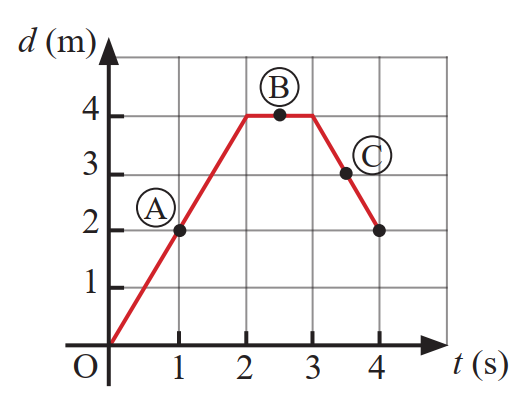
\includegraphics[scale=0.4]{figs/G10Y25B3-21}
		\captionof{figure}{}
		\label{fig:5.3}
	\end{center}
	\loigiai{
		Tốc độ tức thời tại một thời điểm chính là độ dốc của tiếp tuyến với đồ thị ($d$-$t$) tại điểm đó. Trong chuyển động thẳng đều, tốc độ tức thời bằng tốc độ trung bình trên đoạn đó, và bằng giá trị tuyệt đối của hệ số góc của đoạn thẳng trên đồ thị độ dịch chuyển – thời gian.
		\begin{itemize}
			\item Tốc độ tức thời tại $A$ (tại $t=\SI{1}{s}$): Đây là đoạn từ $t=\SI{0}{s}$ đến $t=\SI{1}{s}$.
			$$v_A=\dfrac{\left|d_A - d_0\right|}{t_A - t_0}=\dfrac{\left|2-0\right|}{1-0}=\SI{2}{m/s}.$$
			\item Tốc độ tức thời tại điểm $B$ (tại $t=\SI{3}{s}$): Đây là đoạn từ $t=\SI{2}{s}$ đến $t=\SI{3}{s}$ (hoặc rộng hơn là từ $t=\SI{2}{s}$ đến $t=\SI{4}{s}$).
			$$v_B=\dfrac{\left|d_B - d_{t=2\si{s}}\right|}{t_B - t_{t=2\si{s}}}=\dfrac{\left|4-4\right|}{3-2}=\SI{0}{m/s}.$$
			\item Tốc độ tức thời tại điểm $C$ (tại $t=\SI{4}{s}$): Đây là đoạn từ $t=\SI{3}{s}$ đến $t=\SI{4}{s}$ (hoặc rộng hơn là từ $t=\SI{2}{s}$ đến $t=\SI{4}{s}$).
			$$v_C=\dfrac{\left|d_C - d_{t=3\si{s}}\right|}{t_C - t_{t=3\si{s}}}=\dfrac{\left|2-4\right|}{4-3}=\SI{2}{m/s}.$$
		\end{itemize}
	}
\end{vd}

\begin{vd}
	Đồ thị độ dịch chuyển – thời gian trong chuyển động thẳng của một xe ô tô đồ chơi điều khiển từ xa được vẽ ở hình \ref{fig:5.4}.
	\begin{center}
		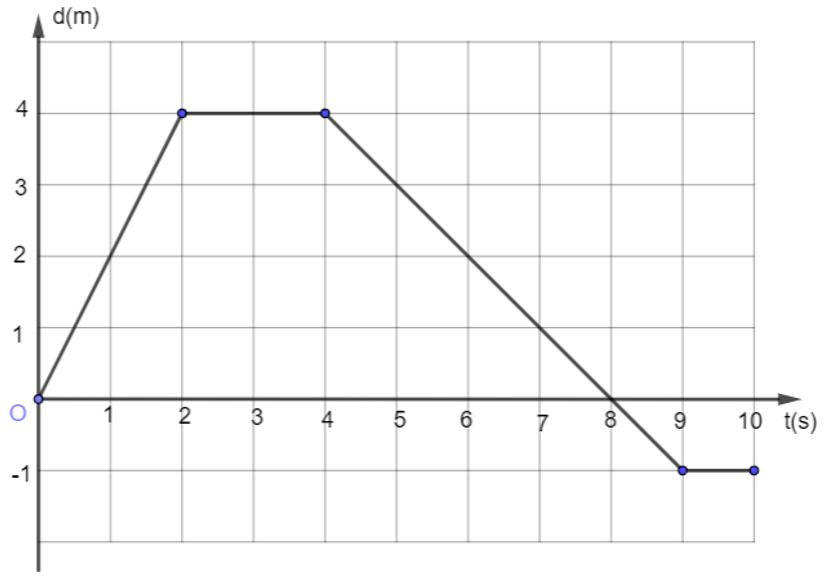
\includegraphics[scale=0.5]{figs/G10Y25B3-20}
		\captionof{figure}{}
		\label{fig:5.4}
	\end{center}
	\begin{enumerate}[label=\alph*)]
		\item Mô tả chuyển động của xe.
		\item Xác định vị trí của xe so với điểm xuất phát của xe ở giây thứ 2, giây thứ 4, giây thứ 8 và giây thứ 10.
		\item Xác định tốc độ và vận tốc của xe trong 2 giây đầu, từ giây 2 đến giây 4 và từ giây 4 đến giây 8.
		\item Xác định quãng đường đi được và độ dịch chuyển của xe sau 10 giây chuyển động. Tại sao giá trị của chúng không giống nhau?
	\end{enumerate}
	\loigiai{
		\begin{enumerate}[label=\alph*)]
			\item **Mô tả chuyển động của xe:**
			\begin{itemize}
				\item **Từ $\SI{0}{s}$ đến $\SI{2}{s}$:** Xe chuyển động thẳng đều theo chiều dương, độ dịch chuyển tăng từ $\SI{0}{m}$ lên $\SI{4}{m}$.
				\item **Từ $\SI{2}{s}$ đến $\SI{4}{s}$:** Xe dừng lại (độ dịch chuyển không đổi, vẫn ở $\SI{4}{m}$).
				\item **Từ $\SI{4}{s}$ đến $\SI{8}{s}$:** Xe chuyển động thẳng đều theo chiều âm (ngược chiều dương), độ dịch chuyển giảm từ $\SI{4}{m}$ về $\SI{0}{m}$ (về vị trí xuất phát).
				\item **Từ $\SI{8}{s}$ đến $\SI{9}{s}$:** Xe tiếp tục chuyển động thẳng đều theo chiều âm, độ dịch chuyển giảm từ $\SI{0}{m}$ xuống $\SI{-1}{m}$.
				\item **Từ $\SI{9}{s}$ đến $\SI{10}{s}$:** Xe dừng lại (độ dịch chuyển không đổi, vẫn ở $\SI{-1}{m}$).
			\end{itemize}
			
			\item **Vị trí của xe so với điểm xuất phát:**
			\begin{itemize}
				\item **Ở giây thứ 2 ($t=\SI{2}{s}$):** Xe cách vị trí xuất phát $\SI{4}{m}$ theo chiều dương ($d=\SI{4}{m}$).
				\item **Ở giây thứ 4 ($t=\SI{4}{s}$):** Xe vẫn cách vị trí xuất phát $\SI{4}{m}$ theo chiều dương ($d=\SI{4}{m}$).
				\item **Ở giây thứ 8 ($t=\SI{8}{s}$):** Xe quay lại vị trí xuất phát ($d=\SI{0}{m}$).
				\item **Ở giây thứ 10 ($t=\SI{10}{s}$):** Xe ở sau vị trí xuất phát $\SI{1}{m}$ ($d=\SI{-1}{m}$).
			\end{itemize}
			
			\item **Tốc độ và vận tốc của xe:**
			\begin{itemize}
				\item **Trong 2 giây đầu (từ $\SI{0}{s}$ đến $\SI{2}{s}$):**
				\begin{itemize}
					\item Độ dịch chuyển: $\Delta d = \SI{4}{m} - \SI{0}{m} = \SI{4}{m}.$
					\item Khoảng thời gian: $\Delta t = \SI{2}{s} - \SI{0}{s} = \SI{2}{s}.$
					\item Vận tốc của xe: $v = \dfrac{\Delta d}{\Delta t} = \dfrac{\SI{4}{m}}{\SI{2}{s}} = \SI{2}{m/s}.$
					\item Tốc độ của xe: $|v| = |\SI{2}{m/s}| = \SI{2}{m/s}.$
				\end{itemize}
				\item **Từ giây 2 đến giây 4 (từ $\SI{2}{s}$ đến $\SI{4}{s}$):**
				\begin{itemize}
					\item Độ dịch chuyển: $\Delta d = \SI{4}{m} - \SI{4}{m} = \SI{0}{m}.$
					\item Khoảng thời gian: $\Delta t = \SI{4}{s} - \SI{2}{s} = \SI{2}{s}.$
					\item Vận tốc của xe: $v = \dfrac{\SI{0}{m}}{\SI{2}{s}} = \SI{0}{m/s}.$
					\item Tốc độ của xe: $|v| = |\SI{0}{m/s}| = \SI{0}{m/s}.$
				\end{itemize}
				\item **Từ giây 4 đến giây 8 (từ $\SI{4}{s}$ đến $\SI{8}{s}$):**
				\begin{itemize}
					\item Độ dịch chuyển: $\Delta d = \SI{0}{m} - \SI{4}{m} = \SI{-4}{m}.$
					\item Khoảng thời gian: $\Delta t = \SI{8}{s} - \SI{4}{s} = \SI{4}{s}.$
					\item Vận tốc của xe: $v = \dfrac{\SI{-4}{m}}{\SI{4}{s}} = \SI{-1}{m/s}.$
					\item Tốc độ của xe: $|v| = |\SI{-1}{m/s}| = \SI{1}{m/s}.$
				\end{itemize}
			\end{itemize}
			
			\item **Quãng đường đi được và độ dịch chuyển sau 10 giây:**
			\begin{itemize}
				\item **Quãng đường đi được ($s$):** Là tổng độ dài đoạn đường xe đã đi được, không xét chiều.
				\begin{itemize}
					\item Từ $\SI{0}{s}$ đến $\SI{2}{s}$: Xe đi được $\SI{4}{m}$.
					\item Từ $\SI{2}{s}$ đến $\SI{4}{s}$: Xe đi được $\SI{0}{m}$.
					\item Từ $\SI{4}{s}$ đến $\SI{8}{s}$: Xe đi được $\SI{4}{m}$ (từ $\SI{4}{m}$ về $\SI{0}{m}$).
					\item Từ $\SI{8}{s}$ đến $\SI{9}{s}$: Xe đi được $\SI{1}{m}$ (từ $\SI{0}{m}$ về $\SI{-1}{m}$).
					\item Từ $\SI{9}{s}$ đến $\SI{10}{s}$: Xe đi được $\SI{0}{m}$.
				\end{itemize}
				Tổng quãng đường xe đi được là $s = \SI{4}{m} + \SI{0}{m} + \SI{4}{m} + \SI{1}{m} + \SI{0}{m} = \SI{9}{m}.$
				
				\item **Độ dịch chuyển ($d$):** Là sự thay đổi vị trí của vật, bằng vị trí cuối trừ vị trí đầu.
				Vị trí ban đầu ($t=\SI{0}{s}$): $d_0 = \SI{0}{m}$.
				Vị trí cuối cùng ($t=\SI{10}{s}$): $d_{10} = \SI{-1}{m}$.
				Độ dịch chuyển sau $\SI{10}{s}$: $d = d_{10} - d_0 = \SI{-1}{m} - \SI{0}{m} = \SI{-1}{m}.$
			\end{itemize}
			
			**Tại sao giá trị của chúng không giống nhau?**
			Giá trị của quãng đường đi được ($\SI{9}{m}$) và độ dịch chuyển ($\SI{-1}{m}$) không giống nhau vì vật đã **đổi chiều chuyển động** trong quá trình di chuyển (từ $\SI{4}{s}$ đến $\SI{9}{s}$ xe chuyển động ngược lại so với ban đầu).
			\begin{itemize}
				\item **Quãng đường đi được** là tổng chiều dài quỹ đạo mà vật đã đi, luôn là một giá trị không âm và chỉ phụ thuộc vào lộ trình.
				\item **Độ dịch chuyển** là một đại lượng vectơ, chỉ phụ thuộc vào vị trí ban đầu và vị trí cuối cùng của vật. Nó có thể dương, âm hoặc bằng 0, và cho biết cả khoảng cách lẫn hướng so với điểm xuất phát.
			\end{itemize}
			Khi vật chuyển động thẳng và không đổi chiều, độ lớn của quãng đường đi được và độ dịch chuyển sẽ bằng nhau. Tuy nhiên, khi vật đổi chiều, tổng quãng đường sẽ lớn hơn độ lớn của độ dịch chuyển.
		\end{enumerate}}
	\end{vd}
\begin{dang}{Xây dựng đồ thị tọa độ - thời gian, chọn tỉ xích, lập bảng giá trị tương ứng cho một vật chuyển động thẳng đều}
\end{dang}
\begin{vd}
	Vật chuyển động thẳng đều có đồ thị tọa độ - thời gian như hình vẽ. Phương trình chuyển động của vật có dạng nào sau đây?
	\begin{center}
		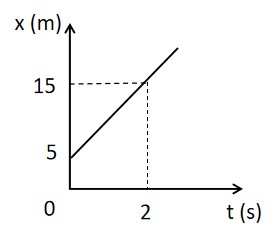
\includegraphics[scale=0.6]{figs/G10Y25B3-22}
	\end{center}
	\choice
	{\True $x=5+5t$.}
	{$x=4t$.}
	{$x=5-5t$.}
	{$x=5+4t$.}
	\loigiai{
		Đồ thị tọa độ - thời gian là một đường thẳng, cho thấy vật chuyển động thẳng đều.
		Từ đồ thị, ta có thể xác định các thông số:
		\begin{itemize}
			\item **Tọa độ ban đầu ($x_0$):** Tại $t = 0$, đồ thị đi qua điểm có tọa độ $x = \SI{5}{m}$. Vậy $x_0 = \SI{5}{m}$.
			\item **Vận tốc ($v$):** Vận tốc của vật được tính bằng độ dốc của đồ thị. Chọn hai điểm rõ ràng trên đồ thị, ví dụ điểm $(\SI{0}{s}, \SI{5}{m})$ và $(\SI{2}{s}, \SI{15}{m})$.
			$$v = \dfrac{\Delta x}{\Delta t} = \dfrac{x_2 - x_1}{t_2 - t_1} = \dfrac{\SI{15}{m} - \SI{5}{m}}{\SI{2}{s} - \SI{0}{s}} = \dfrac{\SI{10}{m}}{\SI{2}{s}} = \SI{5}{m/s}.$$
		\end{itemize}
		
		Phương trình chuyển động thẳng đều có dạng tổng quát là $x = x_0 + vt$.
		Thay các giá trị đã tìm được vào, ta có phương trình chuyển động của vật:
		$$x = 5 + 5t \qquad \left(\si{\meter}, \si{\second}\right).$$
	}
\end{vd}

\begin{vd}
	Hai xe chuyển động đều trên cùng một đường thẳng, cùng chiều. Tốc độ của xe (I) là $\SI{20}{m/s}$, tốc độ của xe (II) là $\SI{10}{m/s}$. Lúc $t=0$, hai xe cách nhau $\SI{200}{m}$. Chọn gốc tọa độ là vị trí của xe (I) lúc $t=0$, chiều dương là chiều chuyển động của hai xe.
	\begin{enumerate}[label=\alph*)]
		\item Viết phương trình chuyển động của mỗi xe.
		\item Vẽ đồ thị chuyển động của hai xe, từ đồ thị hãy xác định thời điểm và nơi gặp nhau của hai xe.
	\end{enumerate}
	\loigiai{
		\begin{enumerate}[label=\alph*)]
			\item **Viết phương trình chuyển động của mỗi xe:**
			Chọn hệ quy chiếu gồm:
			\begin{itemize}
				\item Gốc tọa độ là vị trí của xe (I) lúc $t=0$.
				\item Chiều dương là chiều chuyển động của hai xe.
				\item Mốc thời gian ($t=0$) là lúc hai xe cách nhau $\SI{200}{m}$.
			\end{itemize}
			
			Xác định các thông số cho từng xe:
			\begin{itemize}
				\item **Xe (I):**
				\begin{itemize}
					\item Vị trí ban đầu ($x_{0\text{(I)}}$): Tại gốc tọa độ, nên $x_{0\text{(I)}} = \SI{0}{m}$.
					\item Vận tốc ($v_{\text{(I)}}$): Tốc độ $\SI{20}{m/s}$, chuyển động theo chiều dương, nên $v_{\text{(I)}} = +\SI{20}{m/s}$.
				\end{itemize}
				Phương trình chuyển động của xe (I) là:
				\begin{equation*}
					x_{\text{(I)}}=x_{0\text{(I)}} + v_{\text{(I)}}t = \SI{0}{} + \SI{20}{} \cdot t = 20t\qquad\left(\si{\meter}, \si{\second}\right).
				\end{equation*}
				
				\item **Xe (II):**
				\begin{itemize}
					\item Vị trí ban đầu ($x_{0\text{(II)}}$): Lúc $t=0$, hai xe cách nhau $\SI{200}{m}$ và chuyển động cùng chiều. Do xe (I) ở gốc, xe (II) phải ở vị trí $\SI{200}{m}$ theo chiều dương. Vậy $x_{0\text{(II)}} = \SI{200}{m}$.
					\item Vận tốc ($v_{\text{(II)}}$): Tốc độ $\SI{10}{m/s}$, chuyển động theo chiều dương, nên $v_{\text{(II)}} = +\SI{10}{m/s}$.
				\end{itemize}
				Phương trình chuyển động của xe (II) là:
				\begin{equation*}
					x_{\text{(II)}}=x_{0\text{(II)}} + v_{\text{(II)}}t = \SI{200}{} + \SI{10}{} \cdot t = 200+10t\qquad\left(\si{\meter}, \si{\second}\right).
				\end{equation*}
			\end{itemize}
			
			\item **Vẽ đồ thị chuyển động và xác định thời điểm, nơi gặp nhau:**
			Để vẽ đồ thị, ta lập bảng giá trị tọa độ theo thời gian cho mỗi xe:
			\begin{center}
				\begin{tabular}{|c|c|c|}
					\hline
					$t\ (\si{\second})$ & $x_{\text{(I)}}\ (\si{\meter})$ & $x_{\text{(II)}}\ (\si{\meter})$ \\
					\hline
					0 & 0 & 200 \\
					10 & 200 & 300 \\
					20 & 400 & 400 \\
					30 & 600 & 500 \\
					\hline
				\end{tabular}
			\end{center}
			Đồ thị chuyển động của hai xe là:
			\begin{center}
				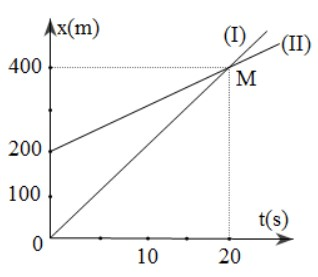
\includegraphics[scale=0.8]{figs/G10Y25B3-23}
			\end{center}
			
			**Xác định thời điểm và nơi gặp nhau từ đồ thị:**
			Hai xe gặp nhau khi tọa độ của chúng bằng nhau, tức là giao điểm của hai đồ thị $x_{\text{(I)}}(t)$ và $x_{\text{(II)}}(t)$.
			Nhìn vào đồ thị, hai đường thẳng cắt nhau tại điểm M có tọa độ $t_M=\SI{20}{s}$ và $x_M=\SI{400}{m}$.
			
			**Kiểm tra bằng phép tính:**
			Hai xe gặp nhau khi $x_{\text{(I)}} = x_{\text{(II)}}$:
			$$20t = 200 + 10t$$
			$$10t = 200$$
			$$t = \dfrac{200}{10} = \SI{20}{s}.$$
			Thay $t = \SI{20}{s}$ vào một trong hai phương trình để tìm vị trí:
			$$x_{\text{(I)}} = 20 \cdot \SI{20}{} = \SI{400}{m}.$$
			
			Vậy, hai xe gặp nhau sau $\SI{20}{s}$ kể từ lúc $t=0$, tại vị trí cách gốc tọa độ (vị trí ban đầu của xe I) một khoảng $\SI{400}{m}$.
		\end{enumerate}	
	}
\end{vd}
\subsection{TRẮC NGHIỆM NHIỀU PHƯƠNG ÁN LỰA CHỌN}
\setcounter{ex}{0}
\Opensolutionfile{ans}[ans/G10Y25B3-TN]
\begin{ex}
	Hãy chọn câu phát biểu đúng?
	\choice
	{Hệ quy chiếu bao gồm hệ toạ độ, mốc thời gian và đồng hồ}
	{Hệ quy chiếu bao gồm vật làm mốc, mốc thời gian và đồng hồ}
	{Hệ quy chiếu bao gồm vật làm mốc, hệ toạ độ, mốc thời gian}
	{\True Hệ quy chiếu bao gồm vật làm mốc, hệ toạ độ, mốc thời gian và đồng hồ}
	\loigiai{
	}
\end{ex}

\begin{ex}
	Kết luận nào sau đây là đúng khi nói về độ dịch chuyển và quãng đường đi được của một vật?
	\choice
	{Độ dịch chuyển và quãng đường đi được đều là đại lượng vô hướng}
	{\True Độ dịch chuyển là đại lượng vectơ còn quãng đường đi được là đại lượng vô hướng}
	{Độ dịch chuyển và quãng đường đi được đều là đại lượng vectơ}
	{Độ dịch chuyển và quãng đường đi được đều là đại lượng không âm}
	\loigiai{
	}
\end{ex}

\begin{ex}
	Một vật bắt đầu chuyển động từ điểm $O$ đến điểm $A$, sau đó chuyển động về điểm $B$. Quãng đường và độ dịch chuyển của vật tương ứng là
	\begin{center}
		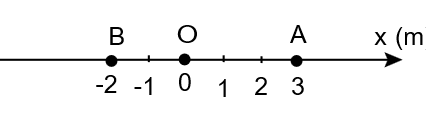
\includegraphics[scale=0.5]{figs/G10Y25B3-7}
	\end{center}
	\choice
	{$\SI{2}{\meter}$; $\SI{-2}{\meter}$}
	{\True $\SI{8}{\meter}$; $\SI{-2}{\meter}$}
	{$\SI{2}{\meter}$; $\SI{2}{\meter}$}
	{$\SI{8}{\meter}$; $\SI{-8}{\meter}$}
	\loigiai{
	}
\end{ex}

\begin{ex}
	Nếu nói “Trái Đất quay quanh Mặt Trời” thì trong câu nói này vật nào được chọn làm mốc
	\choice
	{Cả Mặt Trời và Trái Đất}
	{Trái Đất}
	{Mặt Trăng}
	{\True Mặt Trời}
	\loigiai{
	}
\end{ex}

\begin{ex}
	“Lúc 15 giờ 30 phút hôm qua, xe chúng tôi đang chạy trên quốc lộ 5, cách Hải Dương 10 km”. Việc xác định vị trí của ô tô như trên còn thiếu yếu tố gì?
	\choice
	{Vật làm mốc}
	{\True Chiều dương trên đường đi}
	{Mốc thời gian}
	{Thước đo và đồng hồ}
	\loigiai{
	}
\end{ex}

\begin{ex}
	Trong trường hợp nào dưới đây số chỉ thời điểm mà ta xét trùng với số đo khoảng thời gian trôi?
	\choice
	{Một trận bóng đá diễn ra từ 15 giờ đến 16 giờ 45 phút}
	{Lúc 8 giờ một ô tô khởi hành từ Thành phố Hồ Chí Minh, sau 3 giờ chạy thì xe đến Vũng Tàu}
	{\True Một đoàn tàu xuất phát từ Vinh lúc 0 giờ, đến 8 giờ 05 phút thì đoàn tàu đến Huế}
	{Không có trường hợp nào phù hợp với yêu cầu nêu ra}
	\loigiai{
	}
\end{ex}


\begin{ex}
	Bảng giờ tàu ở bên cho chúng ta biết quãng đường và thời gian mà đoàn tàu SE1 chạy từ ga Huế đến ga Sài Gòn (bỏ qua thời gian tàu đỗ lại các ga) tương ứng là
	\begin{center}
		\begin{tabular}{|c|c|c|}
			\hline
			\thead{Tên ga} & \thead{km} & \thead{SE1}\\
			\hline
			Hà Nội & 0 & 22:15\\
			\hline
			Thanh Hoá & 175& 01:28 (ngày $+1$)\\
			\hline
			Huế & 688 & 11:08 (ngày $+1$)\\
			\hline
			Sài Gòn & 1726 & 06:32 (ngày $+2$)\\
			\hline
		\end{tabular}
	\end{center}
	\choice
	{$\SI{1726}{\kilo\meter}$, 4 giờ 36 phút}
	{$\SI{1726}{\kilo\meter}$, 19 giờ 24 phút}
	{\True $\SI{1038}{\kilo\meter}$, 19 giờ 24 phút}
	{$\SI{1038}{\kilo\meter}$, 4 giờ 36 phút}
	\loigiai{
	}
\end{ex}

\begin{ex}
		\immini{Hai người đi xe đạp từ $A$ đến $C$, người thứ nhất đi theo đường từ $A$ đến $B$, rồi từ $B$ đến $C$; người thứ hai đi thẳng từ $A$ đến $C$. Cả hai đều về đích cùng một lúc.\\
			Hãy chọn kết luận \textbf{sai}.
			\choice
			{Người thứ nhất đi được quãng đường $\SI{8}{\kilo\meter}$}
			{Độ dịch chuyển của người thứ nhất và người thứ hai bằng nhau}
			{\True Độ dịch chuyển và quãng đường đi được của người thứ nhất bằng nhau}
			{Độ dịch chuyển của người thứ nhất là $\SI{5.7}{\kilo\meter}$, hướng $\SI{45}{\degree}$ Đông – Bắc}}{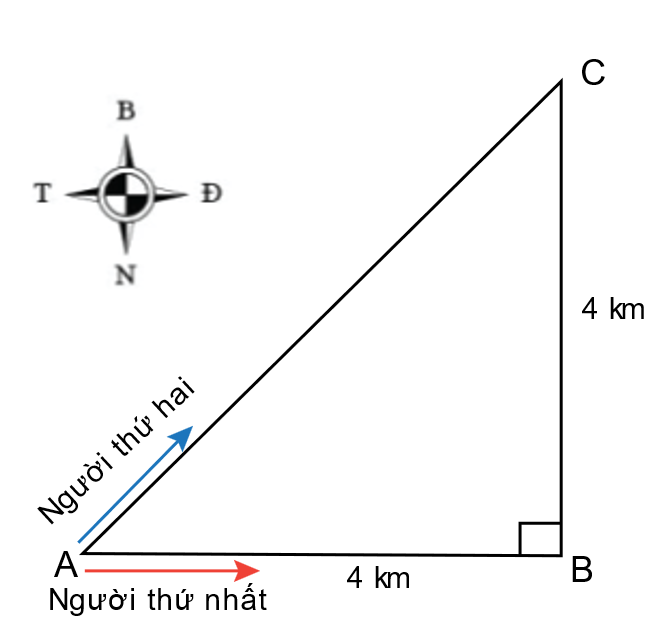
\includegraphics[scale=0.4]{figs/G10Y25B3-6}}
		\loigiai{
		}
\end{ex}

\begin{ex}
	Cho biết Giờ Phối hợp Quốc Tế gọi tắt UTC. So với 0 giờ Quốc Tế, Việt Nam ở múi giờ thứ 7 (UTC+7) và Nhật Bản ở múi giờ thứ 9 (TUC+ 9). Ngày 20/12/2021, máy bay VN300, thuộc hãng hàng không Vietnam Airlines, khởi hành từ Tp. Hồ Chí Minh lúc 0 giờ 20 phút và đến Tp. Tokyo lúc 7 giờ 45 phút, theo giờ địa phương. Thời gian di chuyển của chuyến bay này là
	\choice
	{\True 5 giờ 25 phút}
	{9 giờ 25 phút}
	{7 giờ 25 phút}
	{8 giờ 05 phút}
	\loigiai{
	}
\end{ex}

\begin{ex}
	Chuyến bay từ Thành phố Hồ Chí Minh đi Paris khởi hành lúc 21 giờ 30 phút giờ Hà Nội ngày hôm trước, đến Paris lúc 5 giờ 30 phút sáng hôm sau theo giờ Paris. Biết giờ Paris chậm hơn giờ Hà Nội là 6 giờ. Theo giờ Hà Nội, máy bay đến Paris lúc
	\choice
	{\True 11 giờ 30 phút}
	{14 giờ}
	{12 giờ 30 phút}
	{10 giờ}
	\loigiai{
	}
\end{ex}
\begin{ex}
	Đại lượng đặc trưng cho tính chất nhanh hay chậm của chuyển động là 
	\choice
	{toạ độ}
	{gia tốc}
	{quãng đường đi}
	{\True tốc độ}
	\loigiai{
	}
\end{ex}

\begin{ex}
	Khi nhìn vào tốc kế của ô tô đang chạy, số chỉ trên tốc kế cho ta biết
	\choice
	{gia tốc tức thời của ô tô}
	{vận tốc tức thời của ô tô}
	{\True tốc độ tức thời của ô tô}
	{tốc độ trung bình của ô tô}
	\loigiai{
	}
\end{ex}

\begin{ex}
	Một máy bay phản lực có tốc độ $\SI{700}{\kilo\meter/\hour}$. Nếu muốn bay liên tục trên khoảng cách $\SI{1400}{\kilo\meter}$ thì máy bay phải bay trong thời gian là
	\choice
	{\True $\SI{2}{\hour}$}
	{$\SI{3}{\hour}$}
	{$\SI{2}{\hour}\SI{30}{\minute}$}
	{$\SI{1}{\hour}\SI{30}{\minute}$}
	\loigiai{
		Thời gian máy bay bay quãng đường $\SI{1400}{\kilo\meter}$:
		$$t=\dfrac{s}{v}=\SI{2}{\hour}.$$
	}
\end{ex}

\begin{ex}
	Một xe xuất phát từ lúc 7 giờ 15 phút sáng từ thành phố M, chuyển động thẳng đều tới thành phố N, cách thành phố M $\SI{90}{\kilo\meter}$. Biết tốc độ của xe là $\SI{60}{\kilo\meter/\hour}$, xe đến thành phố N lúc
	\choice
	{9 giờ 45 phút}
	{8 giờ 30 phút}
	{9 giờ 30 phút}
	{\True 8 giờ 45 phút}
	\loigiai{
		Thời gian để xe đi từ M đến N:
		$$\Delta t=\dfrac{s}{v}=\SI{1.5}{\hour}.$$
		Thời điểm xe đến N:
		$$t=\SI{7}{\hour}\SI{15}{\minute}+\Delta t=\SI{8}{\hour}\SI{45}{\minute}.$$
	}
\end{ex}

\begin{ex}
	Một vận động viên chạy cự li $\SI{600}{\meter}$ mất $\SI{74.75}{\second}$. Hỏi vận động viên đó có tốc độ trung bình bao nhiêu?
	\choice
	{\True $\SI{8.03}{\meter/\second}$}
	{$\SI{9.03}{\meter/\second}$}
	{$\SI{10.03}{\meter/\second}$}
	{$\SI{11.03}{\meter/\second}$}
	\loigiai{
		Tốc độ trung bình của vận động viên:
		$$v_\text{tb}=\dfrac{s}{\Delta t}=\SI{8.03}{\meter/\second}.$$
	}
\end{ex}

\begin{ex}
	Trong nội dung thi đấu môn bơi ếch $\SI{100}{\meter}$, một vận động viên đã hoàn thành đường đua với thành tích $\SI{63.25}{\second}$. Tốc độ trung bình của vận động viên này trong giải thi đấu đó là bao nhiêu?
	\choice
	{\True $\SI{1.58}{\meter/\second}$}
	{$\SI{0.63}{\meter/\second}$}
	{$\SI{6.33}{\meter/\second}$}
	{$\SI{36.75}{\meter/\second}$}
	\loigiai{
		Tốc độ trung bình của vận động viên này
		$$v_\text{tb}=\dfrac{s}{t}\approx\SI{1.58}{\meter/\second}.$$
	}
\end{ex}

\begin{ex}
	Một ô tô chạy thử nghiệm trên một đoạn đường thẳng. Cứ $\SI{5}{\second}$ thì có một giọt dầu từ động cơ của ô tô rơi thẳng xuống mặt đường. Hình bên cho thấy mô hình các giọt dầu để lại trên mặt đường. Ô tô chuyển động trên đường này với tốc độ trung bình là
	\begin{center}
		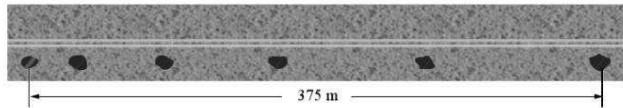
\includegraphics[scale=0.7]{figs/G10Y25B3-15}
	\end{center}
	\choice
	{$\SI{12.5}{\meter/\second}$}
	{\True $\SI{15}{\meter/\second}$}
	{$\SI{30}{\meter/\second}$}
	{$\SI{25}{\meter/\second}$}
	\loigiai{
		Tốc độ trung bình của ô tô:
		$$v_\text{tb}=\dfrac{s}{t}=\dfrac{\SI{375}{\meter}}{\SI{25}{\second}}=\SI{15}{\meter/\second}.$$
	}
\end{ex}

\begin{ex}
	Một chiếc xe ô tô xuất phát từ A lúc 6 giờ sáng, chuyển động thẳng đều tới B, cách A $\SI{120}{\kilo\meter}$. Biết xe tới B lúc 8 giờ 30 phút sáng, tốc độ trung bình của xe là 
	\choice
	{\True $\SI{48}{\kilo\meter/\hour}$}
	{$\SI{45}{\kilo\meter/\hour}$}
	{$\SI{60}{\kilo\meter/\hour}$}
	{$\SI{50}{\kilo\meter/\second}$}
	\loigiai{
		Tốc độ trung bình của xe:
		$$v_\text{tb}=\dfrac{s}{t_2-t_1}=\SI{48}{\kilo\meter/\hour}.$$
	}
\end{ex}

\begin{ex}
	Một xe chuyển động thẳng không đổi chiều, $\SI{1}{\hour}$ đầu xe chạy với tốc độ trung bình $\SI{60}{\kilo\meter/\hour}$ và $\SI{3}{\hour}$ sau xe chạy với tốc độ trung bình $\SI{40}{\kilo\meter/\hour}$. Tính tốc độ trung bình của xe trong suốt thời gian chuyển động.
	\choice
	{$\SI{48}{\kilo\meter/\hour}$}
	{$\SI{40}{\kilo\meter/\hour}$}
	{$\SI{58}{\kilo\meter/\hour}$}
	{\True $\SI{45}{\kilo\meter/\hour}$}
	\loigiai{
		$$v_{tb}=\dfrac{v_1t_1+v_2t_2}{t_1+t_2}=\SI{45}{\kilo\meter/\hour}.$$
	}
\end{ex}

\begin{ex}
	Một người đi xe đạp trên $\dfrac{2}{3}$ đoạn đường đầu với tốc độ trung bình $\SI{10}{\kilo\meter/\hour}$ và $\dfrac{1}{3}$ đoạn đường sau với tốc độ trung bình $\SI{20}{\kilo\meter/\hour}$. Tốc độ trung bình của người đi xe đạp trên cả quãng đường là
	\choice
	{\True $\SI{12}{\kilo\meter/\hour}$}
	{$\SI{15}{\kilo\meter/\hour}$}
	{$\SI{17}{\kilo\meter/\hour}$}
	{$\SI{13.3}{\kilo\meter/\hour}$}
	\loigiai{
		Gọi $s$ là chiều dài đoạn đường
		$$v_{tb}=\dfrac{s}{t_1+t_2}=\dfrac{s}{\dfrac{2s}{3v_1}+\dfrac{s}{3v_2}}=\dfrac{1}{\dfrac{2}{3v_1}+\dfrac{1}{3v_2}}=\SI{12}{\kilo\meter/\hour}.$$
	}
\end{ex}
\begin{ex}
	Khi vật chuyển động thẳng đều cùng chiều dương thì đồ thị $d - t$ của vật có dạng là
	\choice
	{đường thẳng vuông góc với trục $Od$}
	{\True đường thẳng xiên góc đi lên}
	{đường thẳng xiên góc đi xuống}
	{đường thẳng vuông góc với trục $Ot$}
	\loigiai{}
\end{ex}

\begin{ex}
	\immini{Cho đồ thị độ dịch chuyển – thời gian của một vật như hình. Chọn phát biểu đúng.
		\choice
		{Vật đang chuyển động thẳng đều theo chiều dương}
		{Vật đang chuyển động thẳng đều theo chiều âm}
		{\True Vật đang đứng yên}
		{Vật chuyển động thẳng đều theo chiều dương rồi đổi chiều chuyển động ngược lại}}{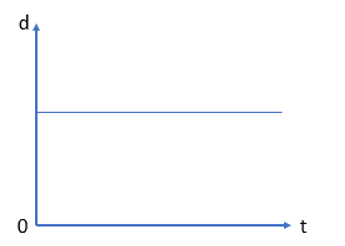
\includegraphics[scale=0.5]{figs/G10Y25B3-24}}
	\loigiai{}
\end{ex}

\begin{ex}
	\immini{Cho đồ thị độ dịch chuyển – thời gian của một vật như hình. Chọn phát biểu đúng.
		\choice
		{Vật đang chuyển động thẳng đều theo chiều dương}
		{Vật đang chuyển động thẳng đều theo chiều âm}
		{Vật đang đứng yên}
		{\True Vật chuyển động thẳng đều theo chiều dương rồi đổi chiều chuyển động ngược lại}}
		{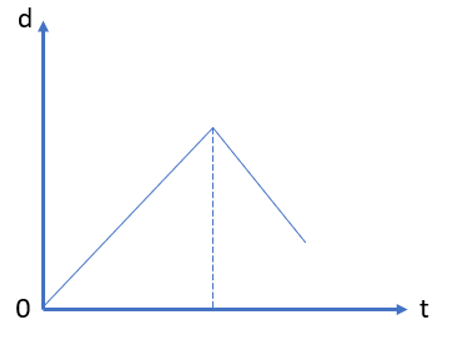
\includegraphics[scale=0.4]{figs/G10Y25B3-25}}
	\loigiai{}
\end{ex}


\begin{ex}
	Đồ thị độ dịch chuyển – thời gian trong chuyển động thẳng của một chất điểm có dạng như hình vẽ.
	\immini{Trong thời gian nào xe chuyển động thẳng đều?
		\choice
		{\True Trong khoảng thời gian từ $0$ đến $t_1$}
		{Trong khoảng thời gian từ $0$ đến $t_2$}
		{Trong khoảng thời gian từ $t_1$ đến $t_2$}
		{Không có lúc nào xe chuyển động thẳng đều}}{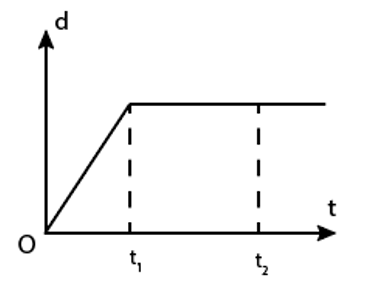
\includegraphics[width=0.5\linewidth]{figs/G10Y25B3-26}}
	\loigiai{}
\end{ex}

\begin{ex}
	{Phương trình chuyển động của một chất điểm dọc theo trục $Ox$ có dạng: $x = 5 + 60t$ ($x$ đo bằng kilomét và $t$ đo bằng giờ). Chất điểm đó xuất phát từ điểm nào và chuyển động với vận tốc bằng bao nhiêu?
		\choice
		{Từ điểm $O$, với vận tốc $\SI{5}{\kilo\meter/\hour}$}
		{Từ điểm $O$, với vận tốc $\SI{60}{\kilo\meter/\hour}$}
		{Từ điểm $M$ cách $O$ $\SI{5}{\kilo\meter}$, với vận tốc $\SI{5}{\kilo\meter/\hour}$}
		{\True Từ điểm $M$ cách $O$ $\SI{5}{\kilo\meter}$, với vận tốc $\SI{60}{\kilo\meter/\hour}$}
	}
	\loigiai{}
\end{ex}

\begin{ex}
	{Phương trình chuyển động của một chất điểm dọc theo $Ox$ có dạng: $x=5t-12$ ($\si{\kilo\meter}$), với $t$ đo bằng giờ. Độ dời của chất điểm từ $\SI{2}{\hour}$ đến $\SI{4}{\hour}$ là
		\choice
		{$\SI{8}{\kilo\meter}$}
		{$\SI{6}{\kilo\meter}$}
		{\True $\SI{10}{\kilo\meter}$}
		{$\SI{2}{\kilo\meter}$}
	}
	\loigiai{}
\end{ex}

\begin{ex}
	{Phương trình chuyển động của một chất điểm dọc theo trục $Ox$ có dạng: $x = 4 -10t$ ($x$ đo bằng kilomét và $t$ đo bằng giờ). Quãng đường đi được của chất điểm sau $\SI{2}{\hour}$ chuyển động là
		\choice
		{$\SI{-20}{\kilo\meter}$}
		{\True $\SI{20}{\kilo\meter}$}
		{$\SI{-8}{\kilo\meter}$}
		{$\SI{8}{\kilo\meter}$}
	}
	\loigiai{}
\end{ex}

\begin{ex}
	\immini{Hình vẽ bên là đồ thị độ dịch chuyển - thời gian của một chiếc xe ô tô chạy từ $A$ đến $B$ trên một đường thẳng. Vận tốc của xe bằng
		\choice
		{\True $\SI{30}{\kilo\meter/\hour}$}
		{$\SI{150}{\kilo\meter/\hour}$}
		{$\SI{120}{\kilo\meter/\hour}$}
		{$\SI{100}{\kilo\meter/\hour}$}}{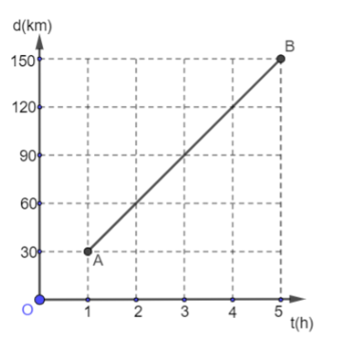
\includegraphics[scale=0.6]{figs/G10Y25B3-27}}
	\loigiai{}
\end{ex}

\begin{ex}\immini{Đồ thị độ dịch chuyển – thời gian của một vật chuyển động như hình vẽ. Vật chuyển động
		\choice
		{\True ngược chiều dương với tốc độ $\SI{20}{\kilo\meter/\hour}$}
		{cùng chiều dương với tốc độ $\SI{20}{\kilo\meter/\hour}$}
		{ngược chiều dương với tốc độ $\SI{60}{\kilo\meter/\hour}$}
		{cùng chiều dương với tốc độ $\SI{60}{\kilo\meter/\hour}$}}{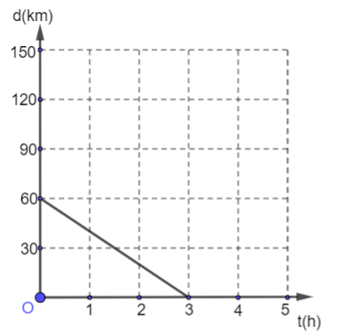
\includegraphics[scale=0.5]{figs/G10Y25B3-28}}

	\loigiai{}
\end{ex}

\begin{ex}
	\immini{Một chất điểm chuyển động trên một đường thẳng. Đồ thị độ dịch chuyển theo thời gian của chất điểm được mô tả như hình vẽ. Tốc độ trung bình của chất điểm trong khoảng thời gian từ 0 đến $\SI{5}{\second}$ là
		\choice
		{$\SI{1.6}{\centi\meter/\second}$}
		{$\SI{6.4}{\centi\meter/\second}$}
		{$\SI{4.8}{\centi\meter/\second}$}
		{\True $\SI{2.4}{\centi\meter/\second}$}}{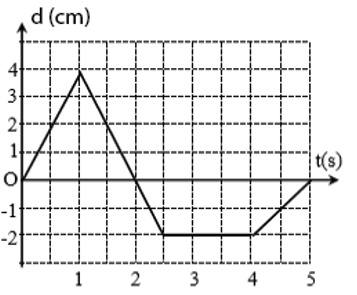
\includegraphics[scale=0.5]{figs/G10Y25B3-29}}
	\loigiai{}
\end{ex}

\begin{ex}
Một người đi bằng thuyền với tốc độ $\SI{2}{m/s}$ về phía đông. Sau khi đi được $\SI{2.2}{\kilo\meter}$, người này lên ô tô đi về phía bắc trong 15 phút với tốc độ $\SI{60}{\kilo\meter/\hour}$. Hãy chọn kết luận \textbf{sai}.
		\choice
		{Tổng quãng đường đã đi là $\SI{17.2}{\kilo\meter}$}
		{Độ dịch chuyển là $\SI{15.2}{\kilo\meter}$}
		{Tốc độ trung bình là $\SI{8.6}{m/s}$}
		{\True Vận tốc trung bình bằng $\SI{8.6}{m/s}$}
	\loigiai{}
\end{ex}

\begin{ex}
Một người bơi dọc theo chiều dài $\SI{100}{m}$ của bể bơi hết $\SI{60}{s}$ rồi quay về lại chỗ xuất phát trong $\SI{70}{s}$. Trong suốt quãng đường đi và về tốc độ trung bình, vận tốc trung bình của người đó lần lượt là
		\choice
		{\True $\SI{1.538}{m/s}$; $\SI{0}{m/s}$}
		{$\SI{1.538}{m/s}$; $\SI{1.876}{m/s}$}
		{$\SI{3.077}{m/s}$; $\SI{2}{m/s}$}
		{$\SI{7.692}{m/s}$; $\SI{2.2}{m/s}$}
	\loigiai{}
\end{ex}

\begin{ex}
Hãy thiết lập phương trình chuyển động của một ô tô chuyển động thẳng đều biết. Ô tô chuyển động theo chiều dương với vận tốc $\SI{10}{m/s}$ và ở thời điểm $\SI{3}{s}$ thì ô tô có tọa độ $\SI{60}{m}$.
		\choice
		{\True $x=30+10t\qquad\left(\si{\meter}, \si{\second}\right)$}
		{$x=20+10t\qquad\left(\si{\meter}, \si{\second}\right)$}
		{$x=10+20t\qquad\left(\si{\meter}, \si{\second}\right)$}
		{$x=40+10t\qquad\left(\si{\meter}, \si{\second}\right)$}
	\loigiai{}
\end{ex}

\begin{ex}
	Hai trạm dừng chân $A$ và $B$ cách nhau $\SI{72}{\kilo\meter}$. Lúc 7h30 sáng, xe ô tô 1 khởi hành từ $A$ chuyển động thẳng đều về $B$ với tốc độ $\SI{36}{\kilo\meter/\hour}$. Nửa giờ sau, xe ô tô 2 chuyển động thẳng đều từ $B$ đến $A$ và gặp ô tô 1 lúc 8 giờ 30 phút. Tìm tốc độ của xe ô tô thứ hai.
		\choice
		{$v_2=\SI{70}{\kilo\meter/\hour}$}
		{\True $v_2=\SI{72}{\kilo\meter/\hour}$}
		{$v_2=\SI{73}{\kilo\meter/\hour}$}
		{$v_2=\SI{74}{\kilo\meter/\hour}$}
	
	\loigiai{}
\end{ex}

\begin{ex}
	Lúc 7 giờ một người đang ở $A$ chuyển động thẳng đều với vận tốc $\SI{10}{m/s}$ đuổi theo người ở $B$ đang chuyển động thẳng đều với vận tốc $\SI{18}{\kilo\meter/\hour}$. Biết $AB =\SI{36}{\kilo\meter}$. Chọn trục tọa độ trùng với quỹ đạo chuyển động, chiều dương là chiều chuyển động, gốc tọa độ tại A, gốc thời gian là lúc $\SI{7}{\hour}$. Thời điểm và vị trí người thứ nhất đuổi kịp người thứ hai là
		\choice
		{lúc $\SI{2}{\hour}$ cách $A$ $\SI{72}{\kilo\meter}$}
		{lúc $\SI{9}{\hour}$ cách $B$ $\SI{36}{\kilo\meter}$}
		{\True lúc $\SI{9}{\hour}$ cách $A$ $\SI{72}{\kilo\meter}$}
		{lúc $\SI{2}{\hour}$ cách $B$ $\SI{36}{\kilo\meter}$}
	\loigiai{}
\end{ex}

\begin{ex}
	Lúc $\SI{10}{\hour}$ có một xe xuất phát từ $A$ đi về $B$ với tốc độ $\SI{50}{\kilo\meter/\hour}$. Lúc 10h30 một xe khác xuất phát từ $B$ đi về $A$ với tốc độ $\SI{80}{\kilo\meter/\hour}$. Cho $AB =\SI{200}{\kilo\meter}$. Lúc $\SI{11}{\hour}$, hai xe cách nhau
		\choice
		{$\SI{100}{\kilo\meter}$}
		{\True $\SI{110}{\kilo\meter}$}
		{$\SI{150}{\kilo\meter}$}
		{$\SI{160}{\kilo\meter}$}
	
	\loigiai{}
\end{ex}

\begin{ex}
	\immini{Hình dưới là đồ thị độ dịch chuyển - thời gian của hai vật chuyển động thẳng cùng hướng. Tỉ lệ vận tốc $\dfrac{v_A}{v_B}$ là
		\choice
		{$\dfrac{3}{1}$}
		{\True $\dfrac{1}{3}$}
		{$\dfrac{\sqrt{3}}{1}$}
		{$\dfrac{1}{\sqrt{3}}$}}{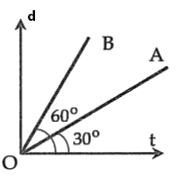
\includegraphics[scale=0.5]{figs/G10Y25B3-30}}
	\loigiai{}
\end{ex}
\Closesolutionfile{ans}
\subsection{TỰ LUẬN VÀ TRẢ LỜI NGẮN}
\setcounter{ex}{0}
\Opensolutionfile{ans}[ans/G10Y25B3-TL]
\begin{ex}
	Khi nào quãng đường và độ di chuyển của một vật có cùng một độ lớn?
	\loigiai{	Chuyển động của vật có quỹ đạo là đường thẳng và không đổi chiều chuyển động.
	}
\end{ex}

\begin{ex}
	Xác định độ dịch chuyển trong các khoảng thời gian liên tiếp bằng nhau của mỗi chuyển động.
	
	\begin{center}
		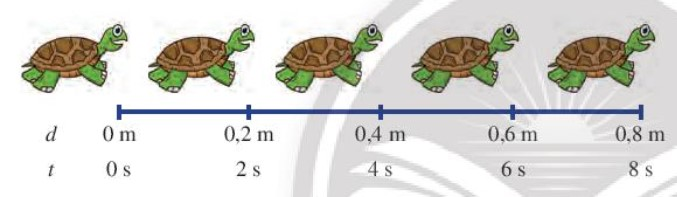
\includegraphics[scale=0.6]{figs/G10Y25B3-8}
	\end{center}
	\loigiai{	
		Độ dịch chuyển trong các khoảng thời gian liên tiếp bằng nhau của mỗi chuyển động
		
		$$\Delta d_1 = x_2 - x_1 = \SI{0,2}{m}.$$
		
		$$\Delta d_2 = x_3 - x_2 = \SI{0,2}{m}.$$
		
		$$\Delta d_3 = x_4 - x_3 = \SI{0,2}{m}.$$
		
		$$\Delta d_4 = x_5 - x_4 = \SI{0,2}{m}.$$
	}
\end{ex}

\begin{ex}
	Hãy xác định các độ dịch chuyển mô tả ở hình trong tọa độ địa lí.
	
	\begin{center}
		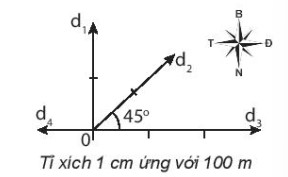
\includegraphics[scale=1]{figs/G10Y25B3-14}
	\end{center}
	\loigiai{	
		Độ dịch chuyển mô tả trên hình là:
		
		$+ d_1 = \SI{200}{m}\ \text{(Bắc)}.$
		
		$+ d_2 = \SI{200}{m}\ \text{(Đông Bắc)}.$
		
		$+ d_3 = \SI{300}{m}\ \text{(Đông)}.$
		
		$+ d_4 = \SI{100}{m}\ \text{(Tây)}.$
	}
\end{ex}

\begin{ex}
	Một ô tô chuyển động trên đường thẳng. Tại thời điểm $t_1$, ô tô ở cách vị trí xuất phát $\SI{5}{km}$. Tại thời điểm $t_2$, ô tô cách vị trí xuất phát $\SI{12}{km}$. Từ $t_1$ đến $t_2$, độ dịch chuyển của ô tô đã thay đổi một đoạn bằng bao nhiêu?
	\loigiai{	
		Từ $t_1$ đến $t_2$, độ dịch chuyển của ô tô thay đổi một đoạn bằng 
		
		$$12-5 = \SI{7}{km}.$$
	}
\end{ex}

\begin{ex}
	Một xe ô tô xuất phát từ tỉnh A, đi đến tỉnh B; rồi lại trở về vị trí xuất phát ở tỉnh A. Xe này đã dịch chuyển, so với vị trí xuất phát một đoạn bằng bao nhiêu? 
	\loigiai{Xe máy này đã dịch chuyển, so với vị trí xuất phát một đoạn là $\SI{0}{km}$.
	}
\end{ex}

\begin{ex}
	Xác định vị trí của vật A trên trục Ox ở hình vẽ tại thời điểm 12h. Biết vật chuyển động thẳng, mỗi giờ đi được $\SI{40}{km}$.
	
	\begin{center}
		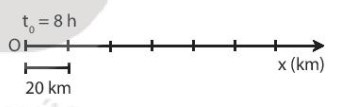
\includegraphics[scale=1]{figs/G10Y25B3-9}
	\end{center}
	\loigiai{	Thời gian vật di chuyển là:
		
		$$12 - 8 = \SI{4}{h}.$$
		
		1 giờ vật di chuyển được $\SI{40}{km}$
		
		$\Rightarrow$ 4 giờ vật di chuyển được: 
		
		$$4 \cdot 40 = \SI{160}{km}.$$
		Tương ứng vật cách gốc toạ độ 8 ô đơn vị.
	}
\end{ex}

\begin{ex}
	Bạn A đi xe đạp từ nhà qua trạm xăng, tới siêu thị mua đồ rồi quay về nhà cất đồ, sau đó đi đến trường. 
	
	\begin{center}
		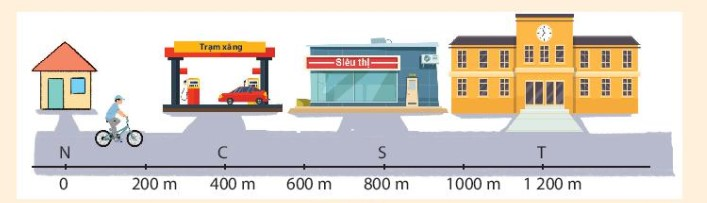
\includegraphics[scale=1]{figs/G10Y25B3-10}
	\end{center}
	Chọn hệ tọa độ có gốc là vị trí nhà bạn A, trục Ox trùng với đường đi từ nhà bạn A đến trường. 
	\begin{enumerate}[label=\alph*)]
		\item Tính quãng đường đi được và độ dịch chuyển của bạn A khi đi từ trạm xăng tới siêu thị.
		\item Tính quãng đường đi được và độ dịch chuyển của bạn A trong cả chuyến đi trên.
	\end{enumerate}
	\loigiai{	
		\begin{enumerate}[label=\alph*)]
			\item Quãng đường bạn A đi từ trạm xăng đến siêu thị là: $$800 - 400 = \SI{400}{m}.$$
			
			Độ dịch chuyển của bạn A từ trạm xăng đến siêu thị là: $$800 - 400 = \SI{400}{m}.$$
			
			\item 
			Quãng đường đi được của bạn A trong cả chuyến đi:
			
			+ Quãng đường bạn A đi từ nhà đến siêu thị là: $\SI{800}{m}.$
			
			+ Quãng đường bạn A quay về nhà cất đồ là: $\SI{800}{m}.$
			
			+ Quãng đường bạn A đi từ nhà đến trường là: $\SI{1200}{m}.$
			
			$\Rightarrow$ Quãng đường đi được của bạn A trong cả chuyến đi là: 	$$ 800 \cdot 2 + 1200 = \SI{2800}{m}.$$ 
			
			Điểm đầu xuất phát của bạn A là nhà, điểm cuối của bạn A là trường.
			
			$\Rightarrow$ Độ dịch chuyển của bạn A là $\SI{1200}{m}.$
			
			Quãng đường đi được và độ dịch chuyển của A trong cả chuyến đi trên là khác nhau. 
		\end{enumerate}
	}
\end{ex}

\begin{ex}
	Hãy so sánh độ lớn của quãng đường đi được và độ dịch chuyển của ba chuyển động. 
	
	\begin{center}
		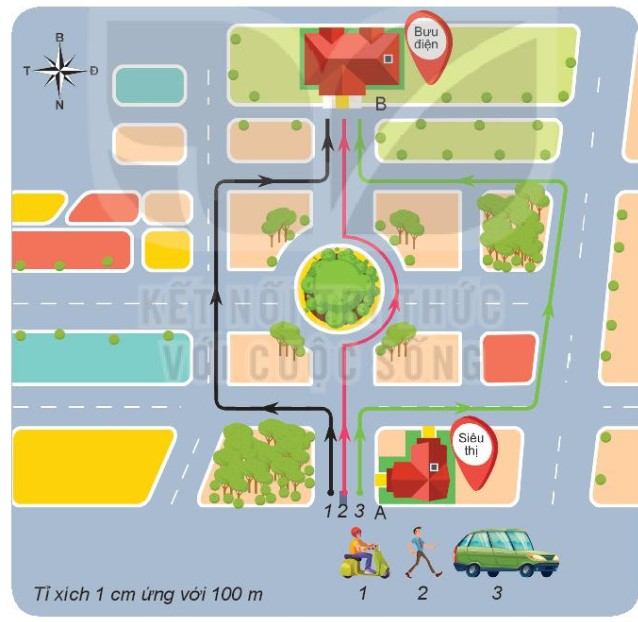
\includegraphics[scale=0.8]{figs/G10Y25B3-11}
	\end{center}
	\loigiai{	
		Quãng đường đi được từ ngắn đến dài: $$2 - 1 - 3.$$
		
		Độ dịch chuyển, ta thấy điểm đầu và điểm cuối của ba chuyển động đều như nhau nên độ dịch chuyển của ba chuyển động bằng nhau.
	}
\end{ex}


\begin{ex}
	Một người lái ô tô đi thẳng $\SI{6}{km}$ theo hướng Tây, sau đó rẽ trái đi thẳng theo hướng Nam $\SI{4}{km}$ rồi quay sang hướng Đông $\SI{3}{km}$. Xác định quãng đường đi được và độ dịch chuyển của ô tô.
	\loigiai{	\begin{center}
			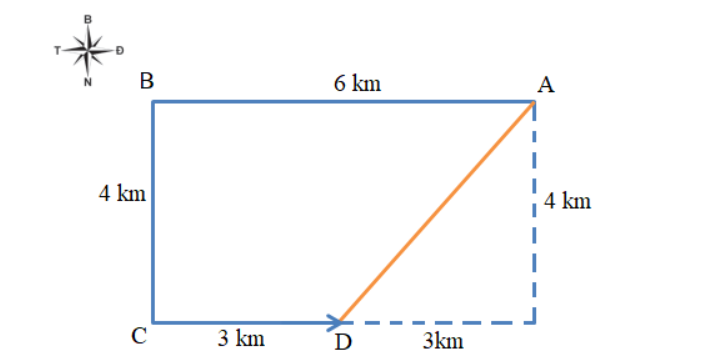
\includegraphics[scale=0.4]{figs/G10Y25B3-12}
		\end{center}
		Quãng đường đi được :
		
		$$s=6+4+3=\SI{13}{km}.$$
		
		Độ dịch chuyển là :
		
		$$d=\sqrt{3^2+4^2}=\SI{5}{\kilo\meter}$$
	}
\end{ex}


\begin{ex}
	Một người bơi ngang từ bờ bên này sang bờ bên kia của một dòng sông rộng $\SI{50}{m}$ có dòng chảy theo hướng từ Bắc xuống Nam. Do nước sông chảy mạnh nên khi sang đến bờ bên kia thì người đó đã trôi xuôi theo dòng nước $\SI{50}{m}$. Xác định độ dịch chuyển của người đó.
	\loigiai{
		\begin{center}
			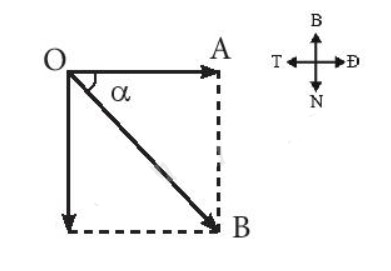
\includegraphics[scale=0.6]{figs/G10Y25B3-13}
		\end{center}
		Người bơi ngang từ bờ bên này sang bên kia theo dự định là OA = $\SI{50}{m}$.
		
		Thực tế, do nước sông chảy mạnh nên vị trí của người đó ở vị trí B, ta có AB = $\SI{50}{m}$.
		
		$\Rightarrow$ Độ dịch chuyển:
		
		$$\Rightarrow\text{OB} = \sqrt{\text{OA}^2 + \text{AB}^2} = \SI{70,7}{m}.$$ 
	}
\end{ex}
\begin{ex}
	Hãy tính tốc độ trung bình ra m/s và km/h của nữ vận động viên tại một số giải thi đấu dựa vào bảng:
	\begin{center}
		\includegraphics[scale=0.5]{figs/G10Y25B3-16}
	\end{center}
	\loigiai{		Tốc độ trung bình của nữ vận động viên tại giải điền kinh quốc gia 2016 là:
		$$v_\text{tb} = \dfrac{s}{t} =\dfrac{100}{\SI{11.64}{}} = \SI{8.6}{m/s} = \SI{30.96}{\kilo\meter/\hour}.$$
		Tốc độ trung bình của nữ vận động viên tại SEA GAME 19, 2017 là:
		$$v_\text{tb} = \dfrac{s}{t} =\dfrac{100}{\SI{11.56}{}} = \SI{8.65}{m/s} = \SI{31.14}{\kilo\meter/\hour}.$$
		Tốc độ trung bình của nữ vận động viên tại SEA GAME 30, 2019 là:
		$$v_\text{tb} = \dfrac{s}{t} =\dfrac{100}{\SI{11.54}{}}= \SI{8.67}{m/s} = \SI{31.19}{\kilo\meter/\hour}.$$
	}
\end{ex}

\begin{ex}
	Một người đi xe máy đi từ ngã tư với tốc độ trung bình $\SI{30}{\kilo\meter/\hour}$ theo hướng Bắc. Sau 3 phút người đó đến vị trí nào trên hình?
	\begin{center}
		\includegraphics[scale=0.5]{figs/G10Y25B3-17}
	\end{center}
	\loigiai{
		Sau 3 phút người đó đi được quãng đường là:
		
		$$s = vt = \SI{30}{\kilo\meter/\hour} \cdot \SI{3}{\minute} = \SI{30}{\kilo\meter/\hour} \cdot \dfrac{\SI{3}{}}{\SI{60}{}}\ \text{h} = \SI{1.5}{\kilo\meter}.$$
		
		Như vậy người đó đến vị trí điểm E.
	}
\end{ex}

\begin{ex}
	Một ô tô chạy liên tục, trong 2 giờ đầu với tốc độ $\SI{80}{\kilo\meter/\hour}$, trong 1 giờ sau chạy với tốc độ $\SI{50}{\kilo\meter/\hour}$. Tốc độ trung bình của xe trong cả quá trình là bao nhiêu?
	\loigiai{
		Đoạn đường đi được trong 2 giờ đầu:
		$$s_1 = v_1 t_1 = \SI{80}{\kilo\meter/\hour} \cdot \SI{2}{\hour} = \SI{160}{\kilo\meter}.$$
		Đoạn đường đi được trong 1 giờ sau:
		$$s_2 = v_2t_2 = \SI{50}{\kilo\meter/\hour} \cdot \SI{1}{\hour} = \SI{50}{\kilo\meter}.$$
		Tốc độ trung bình của xe:
		$$v_\text{tb} = \dfrac{s_1 + s_2}{t_1 + t_2} = \dfrac{\SI{160}{\kilo\meter} + \SI{50}{\kilo\meter}}{\SI{2}{\hour} + \SI{1}{\hour}} = \dfrac{\SI{210}{\kilo\meter}}{\SI{3}{\hour}} = \SI{70}{\kilo\meter/\hour}.$$
	}
\end{ex}

\begin{ex}
	Một người đi xe bắt đầu cho xe chạy trên đoạn đường thẳng: trong 10 giây đầu xe chạy được quãng đường $\SI{50}{m}$, trong 10 giây tiếp theo xe chạy được $\SI{150}{m}$. Tính tốc độ trung bình của xe máy trong khoảng thời gian nói trên.
	\loigiai{
		Tốc độ trung bình của xe máy:
		$$v_\text{tb} = \dfrac{S_1 + S_2}{t_1 + t_2} = \dfrac{\SI{50}{m} + \SI{150}{m}}{\SI{10}{s} + \SI{10}{s}} = \dfrac{\SI{200}{m}}{\SI{20}{s}} = \SI{10}{m/s}.$$
	}
\end{ex}

\begin{ex}
	Một xe máy điện đi nửa đoạn đường đầu tiên với tốc độ trung bình $v_1 = \SI{24}{\kilo\meter/\hour}$ và nửa đoạn đường sau với tốc độ trung bình $v_2 = \SI{40}{\kilo\meter/\hour}$. Tính tốc độ trung bình trên cả đoạn đường.
	\loigiai{Gọi $2s$ là chiều dài cả đoạn đường.
		
		Thời gian đi nửa đoạn đường đầu:
		$$t_1 = \dfrac{s_1}{v_1} = \dfrac{s}{\SI{24}{\kilo\meter/\hour}}.$$
		Thời gian đi nửa đoạn đường cuối:
		$$t_2 = \dfrac{s_2}{v_2} = \dfrac{s}{\SI{40}{\kilo\meter/\hour}}.$$
		Tốc độ trung bình trên cả đoạn đường của xe máy điện:
		$$v = \dfrac{2s}{t_1 + t_2} = \dfrac{2s}{\dfrac{s}{\SI{24}{\kilo\meter/\hour}} + \dfrac{s}{\SI{40}{\kilo\meter/\hour}}} = \dfrac{2}{\dfrac{1}{\SI{24}{\kilo\meter/\hour}} + \dfrac{1}{\SI{40}{\kilo\meter/\hour}}} = \SI{30}{\kilo\meter/\hour}.$$
	}
\end{ex}

\begin{ex}
	Một ô tô chạy trên đoạn đường thẳng từ A đến B phải mất khoảng thời gian $t$. Trong nửa đầu của khoảng thời gian này ô tô có tốc độ là $\SI{60}{\kilo\meter/\hour}$. Trong nửa khoảng thời gian cuối ô tô có tốc độ là $\SI{40}{\kilo\meter/\hour}$. Tính tốc độ trung bình trên cả đoạn AB.
	\loigiai{
		Quãng đường đi được trong nửa thời gian đầu: $s_1 = v_1 \cdot \dfrac{t}{2} = \SI{60}{\kilo\meter/\hour} \cdot \dfrac{t}{2}.$
		Quãng đường đi được trong nửa thời gian cuối: $s_2 = v_2 \cdot \dfrac{t}{2} = \SI{40}{\kilo\meter/\hour} \cdot \dfrac{t}{2}.$
		Tốc độ trung bình:
		$$v_\text{tb} = \dfrac{S}{t} = \dfrac{s_1 + s_2}{t} = \dfrac{v_1\cdot\dfrac{t}{2}+v_2\cdot\dfrac{t}{2}}{t}=\dfrac{v_1 + v_2}{2} =\dfrac{\SI{60}{\kilo\meter/\hour} + \SI{40}{\kilo\meter/\hour}}{2} = \SI{50}{\kilo\meter/\hour}.$$		
	}
\end{ex}

\begin{ex}
	Một người đi xe đạp từ A đến B với tốc độ $\SI{12}{\kilo\meter/\hour}$ trong $\dfrac{1}{3}$ quãng đường, và tốc độ $\SI{18}{\kilo\meter/\hour}$ trong $\dfrac{2}{3}$ quãng đường còn lại. Tính tốc độ trung bình của người đó trên cả đoạn đường AB.
	\loigiai{
		Gọi $S$ là tổng quãng đường AB.
		Thời gian đi $\dfrac{1}{3}$ quãng đường đầu:
		$$t_1 = \dfrac{S/3}{v_1} = \dfrac{S}{3 \cdot \SI{12}{\kilo\meter/\hour}} = \dfrac{S}{\SI{36}{\kilo\meter/\hour}}.$$
		Thời gian đi $\dfrac{2}{3}$ quãng đường còn lại:
		$$t_2 = \dfrac{2S/3}{v_2} = \dfrac{2S}{3 \cdot \SI{18}{\kilo\meter/\hour}} = \dfrac{2S}{\SI{54}{\kilo\meter/\hour}} = \dfrac{S}{\SI{27}{\kilo\meter/\hour}}.$$
		Tốc độ trung bình của người đó:
		$$v_\text{tb} = \dfrac{S}{t_1 + t_2} = \dfrac{S}{\dfrac{S}{\SI{36}{\kilo\meter/\hour}} + \dfrac{S}{\SI{27}{\kilo\meter/\hour}}} = \dfrac{1}{\dfrac{1}{\SI{36}{\kilo\meter/\hour}} + \dfrac{1}{\SI{27}{\kilo\meter/\hour}}} \approx \SI{15.43}{\kilo\meter/\hour}.$$
	}
\end{ex}

\begin{ex}
	Một chiếc thuyền cao tốc đi từ bến A đến bến B. Trong $\dfrac{2}{3}$ thời gian đầu tốc độ của thuyền là $v_1 = \SI{45}{\kilo\meter/\hour}$, thời gian còn lại thuyền chuyển động với tốc độ $v_2$ bằng bao nhiêu để tốc độ trung bình của nó trên cả quãng đường AB là $v = \SI{48}{\kilo\meter/\hour}$?
	\loigiai{
		Gọi $t$ là tổng thời gian thuyền di chuyển.
		Quãng đường đi được trong $\dfrac{2}{3}$ thời gian đầu: $s_1 = v_1 \cdot \dfrac{2t}{3} = \SI{45}{\kilo\meter/\hour} \cdot \dfrac{2t}{3} = \SI{30}{\kilo\meter/\hour} \cdot t.$
		Quãng đường đi được trong thời gian còn lại ($\dfrac{1}{3}$ thời gian): $s_2 = v_2 \cdot \dfrac{t}{3}.$
		Tốc độ trung bình của thuyền trên đoạn đường AB:
		$$v_\text{tb}=\dfrac{s_1 + s_2}{t} = \dfrac{\SI{30}{\kilo\meter/\hour} \cdot t + v_2 \cdot \dfrac{t}{3}}{t}=\SI{30}{\kilo\meter/\hour}+\dfrac{v_2}{3}.$$
		Theo đề bài, $v_\text{tb} = \SI{48}{\kilo\meter/\hour}$.
		$$\SI{48}{\kilo\meter/\hour} = \SI{30}{\kilo\meter/\hour}+\dfrac{v_2}{3}$$
		$$\Rightarrow \dfrac{v_2}{3} = \SI{48}{\kilo\meter/\hour} - \SI{30}{\kilo\meter/\hour} = \SI{18}{\kilo\meter/\hour}$$
		$$\Rightarrow v_2=\SI{54}{\kilo\meter/\hour}.$$
	}
\end{ex}

\begin{ex}
	Một người đua xe đạp đi trên $\dfrac{1}{3}$ quãng đường đầu với tốc độ $\SI{25}{\kilo\meter/\hour}$. Tính tốc độ của người đó đi trên đoạn đường còn lại. Biết rằng tốc độ trung bình trên cả đoạn đường là $v_\text{tb} = \SI{20}{\kilo\meter/\hour}$.
	\loigiai{
		Gọi $s$ là tổng chiều dài đoạn đường.
		Thời gian đi $\dfrac{1}{3}$ quãng đường đầu: $t_1 = \dfrac{s/3}{v_1} = \dfrac{s}{3 \cdot \SI{25}{\kilo\meter/\hour}} = \dfrac{s}{\SI{75}{\kilo\meter/\hour}}.$
		Thời gian đi $\dfrac{2}{3}$ quãng đường còn lại: $t_2 = \dfrac{2s/3}{v_2} = \dfrac{2s}{3v_2}.$
		Tốc độ trung bình trên cả đoạn đường:
		$$v_\text{tb}=\dfrac{s}{t_1+t_2}=\dfrac{s}{\dfrac{s}{\SI{75}{\kilo\meter/\hour}}+\dfrac{2s}{3v_2}}=\dfrac{1}{\dfrac{1}{\SI{75}{\kilo\meter/\hour}}+\dfrac{2}{3v_2}}$$
		$$ \SI{20}{\kilo\meter/\hour}=\dfrac{1}{\dfrac{1}{\SI{75}{\kilo\meter/\hour}}+\dfrac{2}{3v_2}}$$
		$$\Rightarrow \dfrac{1}{\SI{75}{\kilo\meter/\hour}}+\dfrac{2}{3v_2} = \dfrac{1}{\SI{20}{\kilo\meter/\hour}}$$
		$$\dfrac{2}{3v_2} = \dfrac{1}{\SI{20}{\kilo\meter/\hour}} - \dfrac{1}{\SI{75}{\kilo\meter/\hour}} = \dfrac{15-4}{300}\ \text{h/km} = \dfrac{11}{300}\ \text{h/km}$$
		$$v_2 = \dfrac{2}{3} \cdot \dfrac{300}{11}=\xsi{ \dfrac{200}{11}}{\kilo\meter/\hour}  \approx \SI{18.18}{\kilo\meter/\hour}.$$
	}
\end{ex}

\begin{ex}
	Một ô tô đi trên quãng đường AB với tốc độ trung bình $\SI{54}{\kilo\meter/\hour}$. Nếu giảm tốc độ trung bình đi $\SI{9}{\kilo\meter/\hour}$ thì ôtô đến B trễ hơn dự định 45 phút. Tính quãng đường AB và thời gian dự tính để đi quãng đường đó.
	\loigiai{Gọi $t$ là thời gian dự định để đi quãng đường AB (đơn vị: giờ), $v$ là tốc độ trung bình ban đầu và $s$ là chiều dài quãng đường AB.
		Phương trình chuyển động cho trường hợp đi đúng tốc độ trung bình dự kiến:
		\begin{equation}
			\label{eq:1}
			s=vt=\SI{54}{\kilo\meter/\hour} \cdot t
		\end{equation}
		Khi giảm tốc độ trung bình đi $\SI{9}{\kilo\meter/\hour}$, tốc độ mới là $\SI{54}{\kilo\meter/\hour} - \SI{9}{\kilo\meter/\hour} = \SI{45}{\kilo\meter/\hour}$.
		Thời gian đến B trễ hơn dự định 45 phút, tức là $t + \SI{45}{\minute} = t + \dfrac{\SI{45}{}}{\SI{60}{}}\ \text{h} = t + \SI{0.75}{\hour}$.
		Phương trình chuyển động cho trường hợp đi chậm hơn:
		\begin{equation}
			\label{eq:2}
			s=\left(\SI{54}{\kilo\meter/\hour}- \SI{9}{\kilo\meter/\hour}\right)\left(t+\SI{0.75}{\hour}\right)=\SI{45}{\kilo\meter/\hour}\left(t+\SI{0.75}{\hour}\right)
		\end{equation}
		Từ phương trình (\ref{eq:1}) và phương trình (\ref{eq:2}), ta có:
		$$\SI{54}{\kilo\meter/\hour} \cdot t = \SI{45}{\kilo\meter/\hour}\left(t+\SI{0.75}{\hour}\right)$$
		$$54t = 45t + 45 \cdot 0.75$$
		$$9t = 33.75$$
		$$t = \dfrac{33.75}{9} = \SI{3.75}{\hour}.$$
		Thời gian dự tính để đi quãng đường đó là $\SI{3.75}{\hour}$.
		
		Chiều dài quãng đường AB: $s=\SI{54}{\kilo\meter/\hour} \cdot \SI{3.75}{\hour}=\SI{202.5}{\kilo\meter}$.
	}
\end{ex}

\begin{ex}
	Một cậu bé dắt chó đi dạo về nhà, khi còn cách nhà $\SI{10}{m}$, con chó chạy về nhà với tốc độ $\SI{5}{m/s}$. Vừa đến nhà nó lại chạy ngay lại với tốc độ $\SI{3}{m/s}$. Tính tốc độ trung bình của chú chó trong quãng đường đi được kể từ lúc chạy về nhà đến lúc gặp lại cậu bé, biết cậu bé đi đều với tốc độ $\SI{1}{m/s}$.
	\loigiai{
		Thời gian chú chó chạy từ vị trí cách nhà $\SI{10}{m}$ về đến nhà là:
		$$t_1 = \dfrac{s_1}{v_c} = \dfrac{\SI{10}{m}}{\SI{5}{m/s}} = \SI{2}{s}.$$
		Trong thời gian $t_1$ đó, cậu bé đi được quãng đường là:
		$$s_n = t_1 \cdot v_n = \SI{2}{s} \cdot \SI{1}{m/s} = \SI{2}{m}.$$
		Khoảng cách từ cậu bé đến nhà lúc đó (khi chó đã về đến nhà) là:
		$$s' = \SI{10}{m} - s_n = \SI{10}{m} - \SI{2}{m} = \SI{8}{m}.$$
		Sau đó, chó chạy ngược lại gặp cậu bé. Cậu bé và chó chuyển động ngược chiều về phía nhau.
		Thời gian chú chó chạy từ nhà tới lúc gặp lại cậu bé là:
		$$t_2 = \dfrac{s'}{v_c + v_n} = \dfrac{\SI{8}{m}}{\SI{3}{m/s} + \SI{1}{m/s}} = \dfrac{\SI{8}{m}}{\SI{4}{m/s}} = \SI{2}{s}.$$
		Quãng đường chú chó đã quay lại một đoạn là:
		$$s_2 = v_c \cdot t_2 = \SI{3}{m/s} \cdot \SI{2}{s} = \SI{6}{m}.$$
		Tổng quãng đường chú chó đã đi được kể từ lúc chạy về nhà đến lúc gặp lại cậu bé là:
		$$S_{\text{chó}} = s_1 + s_2 = \SI{10}{m} + \SI{6}{m} = \SI{16}{m}.$$
		Tổng thời gian chú chó chuyển động trong quá trình này là:
		$$T_{\text{chó}} = t_1 + t_2 = \SI{2}{s} + \SI{2}{s} = \SI{4}{s}.$$
		Tốc độ trung bình của chú chó trong quãng đường đi được kể từ lúc chạy về nhà đến lúc gặp lại cậu bé là: 
		$$v_{\text{tb}} = \dfrac{S_{\text{chó}}}{T_{\text{chó}}} = \dfrac{\SI{16}{m}}{\SI{4}{s}} = \SI{4}{m/s}.$$
	}
\end{ex}

\begin{ex}
	Một người đi xe máy chuyển động trên đường thẳng theo 3 giai đoạn: Giai đoạn 1 chuyển động với tốc độ không đổi $v_1 = \SI{30}{\kilo\meter/\hour}$ trong $\SI{10}{\kilo\meter}$ đầu tiên; giai đoạn 2 chuyển động với tốc độ $v_2 = \SI{40}{\kilo\meter/\hour}$ trong 30 phút; giai đoạn 3 chuyển động trên đoạn đường $\SI{4}{\kilo\meter}$ trong 10 phút. Tính tốc độ trung bình trên cả đoạn đường.
	\loigiai{
		Thời gian xe máy chuyển động giai đoạn 1:
		$$t_1 = \dfrac{s_1}{v_1} = \dfrac{\SI{10}{\kilo\meter}}{\SI{30}{\kilo\meter/\hour}} = \dfrac{1}{3}\ \text{h}.$$
		Quãng đường giai đoạn 2:
		$$s_2 = v_2t_2 = \SI{40}{\kilo\meter/\hour} \cdot \SI{30}{\minute} = \SI{40}{\kilo\meter/\hour} \cdot \dfrac{30}{60}\ \text{h} = \SI{20}{\kilo\meter}.$$
		Thời gian giai đoạn 3: $\SI{10}{\minute} = \dfrac{10}{60}\ \text{h} = \dfrac{1}{6}\ \text{h}.$
		
		Tổng quãng đường đã đi:
		$$s = s_1 + s_2 + s_3 = \SI{10}{\kilo\meter} + \SI{20}{\kilo\meter} + \SI{4}{\kilo\meter} = \SI{34}{\kilo\meter}.$$
		Tổng thời gian chuyển động:
		$$t = t_1 + t_2 + t_3 = \dfrac{1}{3}\ \text{h} + \dfrac{30}{60}\ \text{h} + \dfrac{10}{60}\ \text{h} = \dfrac{1}{3}\ \text{h} + \dfrac{1}{2}\ \text{h} + \dfrac{1}{6}\ \text{h} = \dfrac{2+3+1}{6}\ \text{h} = \dfrac{6}{6}\ \text{h} = \SI{1}{\hour}.$$
		Tốc độ trung bình của xe máy trên cả đoạn đường:
		$$v_\text{tb} = \dfrac{s}{t} = \dfrac{\SI{34}{\kilo\meter}}{\SI{1}{\hour}} = \SI{34}{\kilo\meter/\hour}.$$
	}
\end{ex}

\begin{ex}
	Một ô tô chuyển động trên đoạn đường MN. Trong một phần hai quãng đường đầu đi với $v = \SI{40}{\kilo\meter/\hour}$. Trong một phần hai quãng đường còn lại đi trong một phần hai thời gian đầu với $v = \SI{75}{\kilo\meter/\hour}$ và trong một phần hai thời gian cuối đi với $v = \SI{45}{\kilo\meter/\hour}$. Tính tốc độ trung bình trên đoạn MN.
	\loigiai{
		Gọi $S$ là chiều dài đoạn đường MN.
		Nửa quãng đường đầu ($S/2$) đi với tốc độ $v_1 = \SI{40}{\kilo\meter/\hour}$.
		Thời gian đi nửa quãng đường đầu là: $t_1 = \dfrac{S/2}{v_1} = \dfrac{S}{2 \cdot \SI{40}{\kilo\meter/\hour}} = \dfrac{S}{\SI{80}{\kilo\meter/\hour}}.$
		
		Xét nửa quãng đường còn lại ($S/2$). Gọi $t'$ là tổng thời gian đi nửa quãng đường này.
		Trong nửa thời gian đầu ($t'/2$), tốc độ là $v_2 = \SI{75}{\kilo\meter/\hour}$. Quãng đường: $s_{2a} = v_2 \cdot \dfrac{t'}{2}.$
		Trong nửa thời gian cuối ($t'/2$), tốc độ là $v_3 = \SI{45}{\kilo\meter/\hour}$. Quãng đường: $s_{2b} = v_3 \cdot \dfrac{t'}{2}.$
		Tổng quãng đường trong giai đoạn này là $S/2 = s_{2a} + s_{2b} = v_2 \cdot \dfrac{t'}{2} + v_3 \cdot \dfrac{t'}{2} = \dfrac{t'}{2}(v_2 + v_3).$
		Tốc độ trung bình trong nửa quãng đường cuối (từ đây ta có thể tính tốc độ trung bình cho nửa sau):
		$$v_{\text{tb2}}=\dfrac{s_{2a}+s_{2b}}{t'} = \dfrac{\dfrac{t'}{2}(v_2+v_3)}{t'} = \dfrac{v_2+v_3}{2} = \dfrac{\SI{75}{\kilo\meter/\hour}+\SI{45}{\kilo\meter/\hour}}{2} = \dfrac{\SI{120}{\kilo\meter/\hour}}{2} = \SI{60}{\kilo\meter/\hour}.$$
		Thời gian đi nửa quãng đường cuối là: $t_2 = \dfrac{S/2}{v_{\text{tb2}}} = \dfrac{S/2}{\SI{60}{\kilo\meter/\hour}} = \dfrac{S}{\SI{120}{\kilo\meter/\hour}}.$
		
		Tổng thời gian đi trên cả đoạn MN là: $T = t_1 + t_2 = \dfrac{S}{\SI{80}{\kilo\meter/\hour}} + \dfrac{S}{\SI{120}{\kilo\meter/\hour}} = S \left( \dfrac{1}{80} + \dfrac{1}{120} \right)\ \text{h/km} = S \left( \dfrac{3+2}{240} \right)\ \text{h/km} = S \cdot \dfrac{5}{240}\ \text{h/km} = \dfrac{S}{\SI{48}{\kilo\meter/\hour}}.$
		Tốc độ trung bình trên cả đoạn MN:
		$$v_\text{tb}=\dfrac{S}{T} = \dfrac{S}{S/\SI{48}{\kilo\meter/\hour}} = \SI{48}{\kilo\meter/\hour}.$$
	}
\end{ex}

\begin{ex}
	Một người đi xe máy trên một đoạn đường thẳng AB. Trên một phần ba đoạn đường đầu đi với $v_1 = \SI{30}{\kilo\meter/\hour}$, một phần ba đoạn đường tiếp theo với $v_2 = \SI{36}{\kilo\meter/\hour}$ và một phần ba đoạn đường cuối cùng đi với $v_3= \SI{48}{\kilo\meter/\hour}$. Tính $v_\text{tb}$ trên cả đoạn AB.
	\loigiai{
		Gọi $S$ là tổng chiều dài đoạn đường AB.
		Thời gian đi một phần ba đoạn đường đầu: $t_1 = \dfrac{S/3}{v_1} = \dfrac{S}{3 \cdot \SI{30}{\kilo\meter/\hour}} = \dfrac{S}{\SI{90}{\kilo\meter/\hour}}.$
		Thời gian đi một phần ba đoạn đường tiếp theo: $t_2 = \dfrac{S/3}{v_2} = \dfrac{S}{3 \cdot \SI{36}{\kilo\meter/\hour}} = \dfrac{S}{\SI{108}{\kilo\meter/\hour}}.$
		Thời gian đi một phần ba đoạn đường cuối cùng: $t_3 = \dfrac{S/3}{v_3} = \dfrac{S}{3 \cdot \SI{48}{\kilo\meter/\hour}} = \dfrac{S}{\SI{144}{\kilo\meter/\hour}}.$
		
		Tổng thời gian đi trên cả đoạn đường AB là:
		$$T = t_1 + t_2 + t_3 = S \left( \dfrac{1}{90} + \dfrac{1}{108} + \dfrac{1}{144} \right)\ \text{h/km}.$$
		Tìm bội chung nhỏ nhất của 90, 108, 144.
		$90 = 2 \cdot 3^2 \cdot 5$
		$108 = 2^2 \cdot 3^3$
		$144 = 2^4 \cdot 3^2$
		BCNN($90, 108, 144$) = $2^4 \cdot 3^3 \cdot 5 = 16 \cdot 27 \cdot 5 = 2160.$
		
		$$T = S \left( \dfrac{2160/90}{2160} + \dfrac{2160/108}{2160} + \dfrac{2160/144}{2160} \right)\ \text{h/km} = S \left( \dfrac{24+20+15}{2160} \right)\ \text{h/km} = S \cdot \dfrac{59}{2160}\ \text{h/km}.$$
		Tốc độ trung bình trên cả đoạn đường AB:
		$$v_\text{tb}=\dfrac{S}{T} = \dfrac{S}{S \cdot \dfrac{59}{2160}\ \text{h/km}} = \xsi{\dfrac{2160}{59}}{\kilo\meter/\hour}\approx \SI{36.61}{\kilo\meter/\hour}.$$
	}
\end{ex}
\begin{ex}
	Hãy tính quãng đường đi được, độ dịch chuyển, tốc độ, vận tốc của bạn A khi đi từ nhà đến trường và khi đi từ trường đến siêu thị. Coi chuyển động của bạn A là chuyển động đều và biết cứ $\SI{100}{m}$ bạn A đi hết $\SI{25}{s}$.
	\begin{center}
		\includegraphics[scale=0.9]{figs/G10Y25B3-31}
	\end{center}
	\loigiai{
		Vì bạn A đi từ nhà đến trường là theo 1 hướng, không đổi hướng nên:
		Quãng đường đi được và độ dịch chuyển là như nhau và bằng $\SI{1000}{m}$.
		Vận tốc và tốc độ là như nhau và bằng:
		$$v = \dfrac{d}{t} = \dfrac{\SI{100}{m}}{\SI{25}{s}} = \SI{4}{m/s}.$$
		Tương tự, khi đi từ trường đến siêu thị thì quãng đường và độ dịch chuyển bằng nhau và bằng $\SI{200}{\meter}$.
	}
\end{ex}

\begin{ex}
	Bạn A đi học từ nhà đến trường theo lộ trình ABC. Biết bạn A đi đoạn đường $\text{AB} = \SI{400}{m}$ hết 6 phút, đoạn đường $\text{BC} = \SI{300}{m}$ hết 4 phút. Xác định tốc độ trung bình và vận tốc trung bình của bạn A khi đi từ nhà đến trường.
	\begin{center}
		\includegraphics[scale=1]{figs/G10Y25B3-32}
	\end{center}
	\loigiai{
		Độ dịch chuyển của bạn A đến trường chính là độ dài $\text{AC}$.
		Vì AB vuông góc với BC, áp dụng định lý Pitago:
		$$\text{AC} = \sqrt{(\text{AB})^2 + (\text{BC})^2} = \sqrt{(\SI{400}{m})^2 + (\SI{300}{m})^2} = \sqrt{160000 + 90000}\ \si{m} = \sqrt{250000}\ \si{m} = \SI{500}{m}.$$
		Tổng quãng đường bạn A đã đi:
		$$s = \text{AB} + \text{BC} = \SI{400}{m} + \SI{300}{m} = \SI{700}{m}.$$
		Tổng thời gian chuyển động:
		$$t = \SI{6}{phút} + \SI{4}{phút} = \SI{10}{phút} = \SI{10}{} \cdot \SI{60}{s} = \SI{600}{s}.$$
		Tốc độ trung bình:
		$$v_{\text{tốc độ}} = \dfrac{s}{t} = \dfrac{\SI{700}{m}}{\SI{600}{s}} \approx \SI{1.17}{m/s}.$$
		Vận tốc trung bình:
		$$v_{\text{vận tốc}} = \dfrac{\text{AC}}{t} = \dfrac{\SI{500}{m}}{\SI{600}{s}} \approx \SI{0.83}{m/s}.$$
	}
\end{ex}

\begin{ex}
	Hãy vẽ đồ thị độ dịch chuyển - thời gian trong chuyển động của A theo bảng ghi số liệu vào vở. Trên trục tung (trục độ dịch chuyển) $\SI{1}{cm}$ ứng với $\SI{200}{m}$; trên trục hoành (trục thời gian) $\SI{1}{cm}$ ứng với $\SI{50}{s}$.
	\begin{center}
		\includegraphics[scale=1]{figs/G10Y25B3-33}
	\end{center}
	\loigiai{
		Từ bảng số liệu ta vẽ được đồ thị như hình sau:
		\begin{center}
			\includegraphics[scale=0.6]{figs/G10Y25B3-34}
		\end{center}
	}
\end{ex}

\begin{ex}
	Đồ thị độ dịch chuyển - thời gian của một người đang bơi trong một bể bơi dài $\SI{50}{m}$.
	\begin{center}
		\includegraphics[scale=1]{figs/G10Y25B3-35}
	\end{center}
	\begin{enumerate}[label=\alph*)]
		\item Trong 25 giây đầu mỗi giây người đó bơi được bao nhiêu mét? Tính vận tốc của người đó ra m/s. Từ giây nào đến giây nào người đó không bơi?
		\item Từ giây 35 đến giây 60 người đó bơi theo chiều nào? Trong 20 giây cuối cùng, mỗi giây người đó bơi được bao nhiêu mét? Tính vận tốc của người đó ra m/s.
		\item Xác định độ dịch chuyển và vận tốc của người đó trong cả quá trình bơi.
	\end{enumerate}
	\loigiai{
		\begin{enumerate}[label=\alph*)]
			\item Từ đồ thị, trong 25 giây đầu (từ $\SI{0}{s}$ đến $\SI{25}{s}$), người đó chuyển động thẳng từ vị trí $\SI{0}{m}$ đến $\SI{50}{m}$. Độ dịch chuyển trong 25 giây đầu là $\SI{50}{m}$.
			Mỗi giây người đó bơi được:
			$$\dfrac{\SI{50}{m}}{\SI{25}{s}} = \SI{2}{m/s}.$$
			Vận tốc của người đó trong 25 giây đầu:
			$$v = \dfrac{\Delta d}{\Delta t} = \dfrac{\SI{50}{m} - \SI{0}{m}}{\SI{25}{s} - \SI{0}{s}} = \SI{2}{m/s}.$$
			Từ đồ thị, đoạn từ A đến B (từ giây 25 đến giây 35), độ dịch chuyển không đổi ($\SI{50}{m}$), nghĩa là người đó không bơi. Vậy, người đó không bơi từ giây 25 đến giây 35.
			\item Từ giây 35 đến giây 60, đồ thị đi xuống, nghĩa là độ dịch chuyển giảm. Điều này cho thấy người đó bơi theo chiều ngược lại (ngược chiều dương).
			Trong 20 giây cuối cùng (từ giây 40 đến giây 60):
			\begin{itemize}
				\item Tại $t=\SI{40}{s}$, $d_1 = \SI{45}{m}$.
				\item Tại $t=\SI{60}{s}$, $d_2 = \SI{25}{m}$.
			\end{itemize}
			Trong 20 giây cuối, độ dịch chuyển thay đổi là $\Delta d = d_2 - d_1 = \SI{25}{m} - \SI{45}{m} = \SI{-20}{m}.$
			Quãng đường đi được trong 20 giây cuối: $s = |\Delta d| = |\SI{-20}{m}| = \SI{20}{m}.$
			Mỗi giây người đó bơi được (tốc độ):
			$$\dfrac{\SI{20}{m}}{\SI{20}{s}} = \SI{1}{m/s}.$$
			Vận tốc của người đó trong 20 giây cuối là:
			$$v = \dfrac{\Delta d}{\Delta t} = \dfrac{\SI{25}{m} - \SI{45}{m}}{\SI{60}{s} - \SI{40}{s}} = \dfrac{\SI{-20}{m}}{\SI{20}{s}} = \SI{-1}{m/s}.$$
			\item Trong cả quá trình bơi (từ $\SI{0}{s}$ đến $\SI{60}{s}$):
			\begin{itemize}
				\item Vị trí ban đầu: $d_{\text{bđ}} = \SI{0}{m}$.
				\item Vị trí cuối cùng: $d_{\text{cuối}} = \SI{25}{m}$.
			\end{itemize}
			Độ dịch chuyển của người đó trong cả quá trình bơi:
			$$\Delta d = d_{\text{cuối}} - d_{\text{bđ}} = \SI{25}{m} - \SI{0}{m} = \SI{25}{m}.$$
			Tổng thời gian bơi: $t = \SI{60}{s}$.
			Vận tốc trung bình của người đó trong cả quá trình bơi:
			$$v_{\text{tb}} = \dfrac{\Delta d}{t} = \dfrac{\SI{25}{m}}{\SI{60}{s}} \approx \SI{0.417}{m/s}.$$
		\end{enumerate}
	}
\end{ex}

\Closesolutionfile{ans}\newpage % SANG (4t)
	\section{CHUYỂN ĐỘNG TỔNG HỢP}
\subsection{LÝ THUYẾT TRỌNG TÂM}
\begin{tomtat}
	\subsubsection{Tính tương đối của chuyển động}
	\paragraph{Quỹ đạo có tính tương đối}
		Hình dạng của quỹ đạo của chuyển động trong các hệ quy chiếu khác nhau thì khác nhau.
	\paragraph{Vận tốc có tính tương đối}
	Vận tốc của chuyển động với các hệ quy chiếu khác nhau thì khác nhau. 
	\subsubsection{Hệ quy chiếu đứng yên và hệ quy chiếu chuyển động}
	\begin{dn}
		\begin{itemize}
			\item \textbf{Hệ quy chiếu đứng yên:} là hệ quy chiếu gắn với vật làm mốc được quy ước là đứng yên.\\
			\textit{\textbf{Ví dụ:}} Hệ quy chiếu gắn với sân ga, hệ quy chiếu gắn với bờ sông, \dots
			\item \textbf{Hệ quy chiếu chuyển động:} là hệ quy chiếu gắn với vật làm gốc chuyển động so với hệ quy chiếu đứng yên.\\
			\textit{\textbf{Ví dụ:}} hệ quy chiếu gắn với tàu hoà đang chuyển động, hệ quy chiếu gắn với dòng nước đang trôi, \dots
		\end{itemize}
	\end{dn}
	\subsubsection{Độ dịch chuyển tổng hợp - Vận tốc tổng hợp}
	Quy ước:
	\begin{itemize}
		\item Vật số 1 (người) là vật chuyển động đang được xét.
		\item Vật số 2 (toa tàu) là vật chuyển động được chọn làm gốc của hệ quy chiếu chuyển động.
		\item Vật số 3 (đường ray) là vật đứng yên được chọn làm gốc của hệ quy chiếu đứng yên
	\end{itemize}
	\begin{center}
		\includegraphics[scale=0.5]{figs/G10Y25B4-1}
	\end{center}
	Khi vật 1 có độ dịch chuyển $\overrightarrow{d_{12}}$ trong hệ quy chiếu chuyển động, đồng thời hệ quy chiếu chuyển động cũng có độ dịch chuyển $\overrightarrow{d_{23}}$ so với hệ quy chiếu đứng yên. Do đó, độ dịch chuyển tổng hợp:
	$$\overrightarrow{d_{13}}=\overrightarrow{d_{12}}+\overrightarrow{d_{23}}$$
	Xét trong khoảng thời gian $\Delta t$ rất bé và kết hợp với định nghĩa của vận tốc:
	$$\dfrac{\overrightarrow{d_{13}}}{\Delta t}=\dfrac{\overrightarrow{d_{12}}}{\Delta t}+\dfrac{\overrightarrow{d_{23}}}{\Delta t}$$
	\begin{noidung}{Công thức cộng vận tốc}
			$$\overrightarrow{v_{13}}=\overrightarrow{v_{12}}+\overrightarrow{v_{23}}$$
		Trong đó:
		\begin{itemize}
			\item $\overrightarrow{v_{13}}$: vận tốc tuyệt đối (vận tốc của vật đối với hệ quy chiếu đứng yên);
			\item $\overrightarrow{v_{12}}$: vận tốc tương đối (vận tốc của vật đối với hệ quy chiếu chuyển động);
			\item $\overrightarrow{v_{23}}$: vận tốc kéo theo (vận tốc của hệ quy chiếu chuyển động đối với hệ quy chiếu đứng yên).
		\end{itemize}
	\end{noidung}

	\begin{center}
		\setlength\arrayrulewidth{1.5pt}
		\begin{tabular}{|M{8.85cm}|M{8.85cm}|}
			\hline
			\rowcolor{violet!30!white}\textbf{Trường hợp 1:} $\overrightarrow{v_{12}}\upuparrows \overrightarrow{v_{23}}$ &\textbf{Trường hợp 2:} $\overrightarrow{v_{12}}\uparrow\downarrow \overrightarrow{v_{23}}$\\
			\hline
				\begin{tikzpicture}
				\coordinate (O) at (0,0);
				\coordinate (B) at (2,0);
				\coordinate (C) at (5,0);
				\coordinate (D) at (2.5,0);
				\coordinate (O1) at ($(O)-(0,1cm)$);
				\coordinate (C1) at ($(C)-(0,1cm)$);
				\coordinate (D1) at ($(D)-(0,1cm)$);
				\draw[-stealth, red, line width=2pt] (O) -- (B);
				\draw[-stealth,blue, line width=2pt] (B) -- (C);
				\draw[-stealth,, line width=2pt] (O1) -- (C1);
				\foreach \i in {O,O1}{
					\filldraw[black] (\i) circle (0.5mm);
				}
				\node[label={[red]90:$\overrightarrow{v_{12}}$}] at (B){};	
				\node[label={[blue]90:$\overrightarrow{v_{23}}$}] at (C){};	
				\node[label=90:$\overrightarrow{v_{13}}$] at (D1){};	
			\end{tikzpicture} & 
			\begin{tikzpicture}
				\coordinate (O) at (0,0);
				\coordinate (B) at (4,0);
				\coordinate (C) at (-2,0);
				\coordinate (D) at (2,0);
				\coordinate (E) at (1,0);
				\coordinate (O1) at ($(O)-(0,1cm)$);
				\coordinate (D1) at ($(D)-(0,1cm)$);
				\coordinate (E1) at ($(E)-(0,1cm)$);
				\draw[-stealth, line width=2pt, red] (O) -- (B);
				\draw[-stealth, line width=2pt, blue] (O) -- (C);
				\draw[-stealth, line width=2pt] (O1) -- (D1);
				\foreach \i in {O,O1}{
					\filldraw[black] (\i) circle (0.5mm);
				}
				\node[label={[red]90:$\overrightarrow{v_{12}}$}] at (B){};	
				\node[label={[blue]90:$\overrightarrow{v_{23}}$}] at (C){};	
				\node[label=90:$\overrightarrow{v_{13}}$] at (E1){};	
			\end{tikzpicture}\\
			$$v_{13}=v_{12}+v_{23}$$ & $$v_{13}=\left|v_{12}-v_{23}\right|$$\\
			\hline
			\rowcolor{violet!30!white}\textbf{Trường hợp 3:} $\overrightarrow{v_{12}} \bot \overrightarrow{v_{23}}$ &  \textbf{Trường hợp 4:} $\left(\overrightarrow{v_{12}},\overrightarrow{v_{23}}\right)=\alpha$\\
			\hline
			\begin{tikzpicture}
				\coordinate (O) at (0,0);
				\coordinate (B) at (4,0);
				\coordinate (C) at (0,3);
				\coordinate (D) at (4,3);
				\coordinate (E) at (1,0);
				\coordinate (O1) at ($(O)-(0,1cm)$);
				\coordinate (D1) at ($(D)-(0,1cm)$);
				\coordinate (E1) at ($(E)-(0,1cm)$);
				\draw[-stealth, line width=2pt, red] (O) -- (B);
				\draw[-stealth, line width=2pt, blue] (O) -- (C);
				\draw[-stealth, line width=2pt] (O) -- (D);
				\draw[dashed] (B) -- (D);
				\draw[dashed] (C) -- (D);
				\foreach \i in {O}{
					\filldraw[black] (\i) circle (0.5mm);
				}
				\tkzMarkRightAngle[draw=black,size=.4](B,O,C);
				\node[label={[red,below right]90:$\overrightarrow{v_{12}}$}] at (B){};	
				\node[label={[blue]90:$\overrightarrow{v_{23}}$}] at (C){};	
				\node[label=90:$\overrightarrow{v_{13}}$] at (D){};	
			\end{tikzpicture} &
			\begin{tikzpicture}
				\coordinate (O) at (0,0);
				\coordinate (B) at (4,0);
				\coordinate (C) at (5,3);
				\coordinate (D) at (1,3);
				\draw[-stealth, line width=2pt, red] (O) -- (B);
				\draw[-stealth, line width=2pt, blue] (O) -- (D);
				\draw[-stealth, line width=2pt] (O) -- (C);
				\draw[dashed] (C) -- (D);
				\draw[dashed] (C) -- (B);
				\foreach \i in {O}{
					\filldraw[black] (\i) circle (0.5mm);
				}
				\node[label={[red,below right]90:$\overrightarrow{v_{12}}$}] at (B){};	
				\node[label={[blue]90:$\overrightarrow{v_{23}}$}] at (D){};	
				\node[label=90:$\overrightarrow{v_{13}}$] at (C){};	
				\tkzMarkAngle[size=0.75cm,color=cyan](B,O,D);
				\tkzLabelAngle[color=black,pos=1.0, above](B,O,D){$\alpha$}
			\end{tikzpicture}\\
				$$v_{13}=\sqrt{v^2_{12}+v^2_{23}}$$& 	$$v_{13}=\sqrt{v^2_{12}+v^2_{23}+2v_{12}\cdot v_{23\cdot}\cos\alpha}$$
				Nếu $v_{12}=v_{23}$ thì $v_{13}=2v_{12}\cdot\cos\dfrac{\alpha}{2}$.\\
				\hline
		\end{tabular}
	\end{center}
\end{tomtat}
\subsection{VÍ DỤ MINH HỌA}
\begin{dang}{Phân biệt vật chuyển động và đứng yên trong các hệ quy chiếu khác nhau}
\end{dang}
\begin{vd}
	Một hành khách ngồi trên toa tàu A, nhìn qua cửa sổ thấy toa tàu B bên cạnh và gạch lát sân ga đều chuyển động như nhau. Nếu lấy vật mốc là nhà ga thì:
	\choice
	{Cả hai tàu đều đứng yên}
	{\True Tàu B đứng yên, tàu A chuyển động}
	{Tàu A đứng yên, tàu B chạy}
	{Cả hai tàu đều chạy}
	\loigiai{
		Khi hành khách ngồi trên toa tàu A, mà thấy toa tàu B bên cạnh và gạch lát sân ga đều chuyển động như nhau thì tàu B và sân ga cùng trạng thái chuyển động so với tàu A.
		
		Nếu lấy vật mốc là nhà ga, gạch lát sân ga đứng yên nên tàu B cũng đứng yên. Sân ga chuyển động so với tàu A đồng nghĩa với tàu A chuyển động so với sân ga.
		
		Vậy trong hệ qui chiếu gắn với sân ga (lấy vật mốc là nhà ga), tàu A chuyển động, tàu B đứng yên.
	}
\end{vd}

\begin{vd}
	Hành khách 1 đứng trên toa tàu a, nhìn qua cửa số toa sang hành khách 2 ở toa bên cạnh b. Hai toa tàu đang đỗ trên hai đường tàu song song với nhau trong sân ga. Bỗng 1 thấy 2 chuyển động về phía sau. Tình huống nào sau đây chắc chắn không xảy ra?
	\choice
	{Cả hai toa tàu cùng chạy về phía trước. Toa a chạy nhanh hơn toa b}
	{\True Cả hai toa tàu cùng chạy về phía trước. Toa b chạy nhanh hơn toa a}
	{Toa tàu a chạy về phía trước. Toa b đứng yên}
	{Toa tàu a đứng yên. Toa tàu b chạy về phía sau}
	\loigiai{
		Nếu cả hai tàu cùng chạy về phía trước, tàu b chạy nhanh hơn thì hành khách trên tàu b sẽ chuyển động vượt lên trước hành khách trên tàu a, tức là hành khách 2 sẽ chuyển động về phía trước so với hành khách 1.
	}
\end{vd}
\begin{dang}{Tính vận tốc tuyệt đối, vận tốc tương đối, vận tốc kéo theo}
	Công thức cộng vận tốc:
	$$\overrightarrow{v_{13}}=\overrightarrow{v_{12}}+\overrightarrow{v_{23}}$$
\end{dang}
% ===============================================================
\begin{vd}
	Một ô tô chạy đều trên một đường thẳng với vận tốc \SI{40}{\kilo\meter/\hour}. Một ô tô B đuổi theo ô tô A với vận tốc \SI{50}{\kilo\meter/\hour}. Xác định vận tốc của:
	\begin{enumerate}[label=\alph*.]
		\item xe ô tô B đối với ô tô A,  
		\item xe ô tô A đối với ô tô B.
	\end{enumerate}
	\loigiai{
		Gọi C là một vật đứng yên trên mặt đất trên mặt đất. Hệ quy chiếu gắn với C là hệ qui chiếu đứng yên. Các giá trị vận tốc mà đề bài cho là vận tốc của xe đối với C. 
		
		Trên hình vẽ, ta thể hiện các vectơ vận tốc của các xe A và B đối với C là các vectơ $\vec{v}_{\text{A,C}}$, $\vec{v}_\text{B,C}$.  
		\begin{center}
			\begin{tikzpicture}
				\coordinate (laxis) at (-2,0);
				\coordinate (C) at (0,0);
				\coordinate (A) at (7,0);
				\coordinate (B) at (1,0);
				\coordinate (va) at ($(A)+(2,0)$);
				\coordinate (vb) at ($(B)+(2.5,0)$);
				\coordinate (raxis) at (10,0);
				\draw[->] (laxis) -- (raxis);
				
				
				\draw[->,ultra thick,blue] (A) -- (va);
				\draw[->,ultra thick,green!60!black] (B) -- (vb);
				\node[below=2mm] at (A) {xe A};
				\node[below=2mm] at (B) {xe B};
				\node[below=2mm] at (C) {C};
				\node[right] at (raxis) {$x$};
				\node[above=1mm] at (va) {$\vec{v}_{\text{A,C}}$};
				\node[above=1mm] at (vb) {$\vec{v}_{\text{B,C}}$};
				\coordinate (va2) at ($(A)-(2,0)$);
				\coordinate (vb2) at ($(B)-(2.5,0)$);
				\filldraw (C) circle (4pt);
				\foreach \i in {B,A}
				{
					\filldraw (\i) circle (4pt);
				}
			\end{tikzpicture}
		\end{center}
		\begin{enumerate}[label=\alph*.]
			\item Vận tốc của ô tô B đối với ô tô A là: 	$$\vec{v}_{\textrm{B,A}}=\vec{v}_{\textrm{B,C}}+\vec{v}_{\textrm{C,A}}==\vec{v}_{\textrm{B,C}}-\vec{v}_{\textrm{A,C}},$$
			Chọn chiều dương là chiều chuyển động của hai ô tô.
			Chiếu lên chiều dương, ta được:
			$$v_{\textrm{B,A}}=v_{\textrm{B,C}}-v_{\textrm{A,C}}= 50\, \textrm{km/h}-40\, \textrm{km/h} = 10\, \textrm{km/h}.$$
			\item Vận tốc của ô tô A đối với ô tô B: 	$$\vec{v}_{\textrm{A,B}}=\vec{v}_{\textrm{A,C}}+\vec{v}_{\textrm{C,B}}=\vec{v}_{\textrm{A,C}}-\vec{v}_{\textrm{B,C}}$$
			Chiếu lên chiều dương, ta được:
			$$v_{\textrm{A,B}}=v_{\textrm{A,C}}-v_{\textrm{B,C}}= 40\, \textrm{km/h}-50\, \textrm{km/h} = -10\, \textrm{km/h}.$$
			
			$\bullet$ \textbf{Lưu ý:} Ta cũng có thể suy ra kết quả này từ kết quả câu \textit{a} bằng:
			$$v_{\textrm{A,B}}=-v_{\textrm{B,A}}=-\SI{10}{\kilo\meter/\hour}.$$
		\end{enumerate}	
	}
\end{vd}
\begin{vd}
	Ô tô A chạy đều trên một đường thẳng với tốc độ $\SI{40}{\kilo\meter/\hour}$. Một ô tô B chạy theo phương vuông góc với ô tô A có tốc độ $\SI{30}{\kilo\meter/\hour}$. Xác định tốc độ của xe ô tô B đối với ô tô A.
	\loigiai{
		Ta kí hiệu A là ô tô A, B là ô tô B, C là đất.
		Vận tốc của ô tô B đối với ô tô A: 	$$\vec{v}_{\textrm{B,A}}=\vec{v}_{\textrm{B,C}}+\vec{v}_{\textrm{C,A}}.$$
		Vectơ $\vec{v}_{\textrm{C,A}}=-\vec{v}_{\textrm{A,C}}$ là vectơ cùng độ lớn nhưng ngược hướng với vectơ $\vec{v}_{\textrm{A,C}}$, được biểu diễn bằng vectơ màu đỏ trong hình.
		\begin{center}
			\begin{tikzpicture}[scale=0.8]
				\coordinate (laxis) at (0,0);
				\coordinate (daxis) at (0,0);
				\coordinate (A) at (2,0);
				\coordinate (B) at (0,1);
				\coordinate (va) at ($(A)+(2,0)$);
				\coordinate (vb) at ($(B)+(0,1.5)$);
				\coordinate (raxis) at (5,0);
				\coordinate (uaxis) at (0,3.5);
				\draw[-] (laxis) -- (raxis);
				\draw[-] (daxis) -- (uaxis);
				\draw[->,ultra thick,blue] (A) -- (va);
				\draw[->,ultra thick,green!60!black] (B) -- (vb);
				\node[above=2mm] at (A) {xe A};
				\node[left=2mm] at (B) {xe B};
				%\node[right] at (raxis) {$x$};
				%\node[above] at (uaxis) {$y$};
				\node[below=1mm] at (va) {$\vec{v}_{\text{A,C}}$};
				\node[right=1mm] at (vb) {$\vec{v}_{\text{B,C}}$};
				\coordinate (va2) at ($(A)-(2,0)$);
				\draw[->,ultra thick,red] (A) -- (va2);
				\node[below=1mm] at (va2) {$\vec{v}_{\text{C,A}}$};
				\foreach \i in {B,A}
				{
					\filldraw (\i) circle (2pt);
				}
				\coordinate (O) at (9,1);
				\coordinate (Ou) at ($(O)+(0,1.5)$);
				\coordinate (Ol) at ($(O)-(2,0)$);
				\coordinate (O2) at ($(O)+(-2,1.5)$);
				\draw[->,ultra thick,green!60!black] (O) -- (Ou);
				\draw[->,ultra thick,red] (O) -- (Ol);
				\draw[dashed] (Ou)--(O2);
				\draw[dashed] (Ol)--(O2);
				\draw[->,ultra thick,violet] (O)--(O2);
				\node[below=1mm] at (Ol) {$\vec{v}_{\text{C,A}}$};
				\node[right=1mm] at (Ou) {$\vec{v}_{\text{B,C}}$};
				\node[above left] at (O2) {$\vec{v}_{\text{B,A}}$};
			\end{tikzpicture}
		\end{center}
		
		Do hai ô tô chuyển động theo hai phương vuông góc nhau nên:
		$$v_{\textrm{B,A}}=\sqrt{v_{\textrm{B,C}}^2+v_{\textrm{C,A}}^2}=\sqrt{(\SI{30}{\kilo\meter/\hour})^2+(\SI{40}{\kilo\meter/\hour})^2}=\SI{50}{\kilo\meter/\hour}.$$
	}
\end{vd}
\begin{dang}{Áp dụng công thức cộng vận tốc, tính vận tốc tương đối cùng phương, cùng chiều hoặc ngược chiều với vận tốc kéo theo}
	Khi thuyền chuyển động xuôi dòng:
	$$v_{\text{xd}}=v_{\text{t}}+v_{\text{n}}.$$
	Khi thuyền chuyển động ngược dòng:
	$$v_{\text{nd}}=v_{\text{t}}-v_{\text{n}}.$$
	\end{dang}
\begin{vd}
	Hai bến sông A và B cách nhau $\SI{11.2}{\kilo\meter}$. Một chiếc ca nô phải mất bao nhiêu thời gian để đi từ A đến B rồi trở lại ngay từ B về A. Biết tốc độ của ca nô so với nước không chảy là $v_1=\SI{15}{\kilo\meter/\hour}$ và tốc độ của nước với bờ sông là $v_2=\SI{1}{\kilo\meter/\hour}$.
	\loigiai{
		Ta gọi $v_{\text{xd}}, v_{\text{nd}}$ lần lượt là tốc độ của thuyền đối với bờ khi nó xuôi dòng và ngược dòng.
		
		Tốc độ của thuyền đối với bờ khi thuyền đi xuôi dòng:
		$$v_{\text{xd}}=v_1+v_2 = \SI{16}{\kilo\meter/\hour}.$$
		Thời gian thuyền đi xuôi dòng khi nó đi từ A đến B:
		$$t_{\text{xd}}=\dfrac{\text{AB}}{v_{\text{xd}}}=\dfrac{\SI{11.2}{\kilo\meter}}{\SI{16}{\kilo\meter/\hour}}=\SI{0.7}{\hour}.$$
		Tốc độ của thuyền đối với bờ khi thuyền đi ngược dòng:
		$$v_{\text{nd}}=v_1-v_2 = \SI{14}{\kilo\meter/\hour}.$$
		Thời gian thuyền đi ngược dòng khi nó đi từ B đến A:
		$$t_{\text{nd}}=\dfrac{\text{AB}}{v_{\text{nd}}}=\dfrac{\SI{11.2}{\kilo\meter}}{\SI{14}{\kilo\meter/\hour}}=\SI{0.8}{\hour}.$$
		Tổng thời gian ca nô đi từ A đến B và từ B về A là:
		$$t= t_{\text{xd}}+ t_{\text{nd}}=\SI{0.7}{\hour}+\SI{0.8}{\hour}=\SI{1.5}{\hour}.$$
	}
\end{vd}

\begin{vd}
	Một chiếc thuyền chạy xuôi dòng sông mất $\SI{2}{\hour}$ để chạy thẳng đều từ bến A ở thượng lưu tới bến B ở hạ lưu và phải mất $\SI{3}{\hour}$ khi chạy ngược lại từ bến B về đến bến A. Cho rằng tốc độ của thuyền đối với nước là $v_1=\SI{30}{\kilo\meter/\hour}$, tốc độ của dòng nước đối với bờ sông là $v_2$. Tính khoảng cách AB và $v_2$.
	\loigiai{
		Ta gọi $v_{\text{xd}}, v_{\text{nd}}$ lần lượt là tốc độ của thuyền khi xuôi dòng và ngược dòng.
		
		Tốc độ của thuyền đối với bờ khi thuyền đi xuôi dòng là:
		$$v_{\text{xd}}=v_1+v_2.$$
		Thời gian thuyền đi xuôi dòng khi nó đi từ A đến B:
		\begin{equation*}
			t_{\text{xd}}=\dfrac{\text{AB}}{v_{\text{xd}}}= \dfrac{\text{AB}}{v_1+v_2}\quad \Rightarrow\quad \text{AB}=(v_1+v_2)t_{\text{xd}}
		\end{equation*}
		Tốc độ của thuyền đối với bờ khi thuyền đi ngược dòng là:
		$$v_{\text{nd}}=v_1-v_2.$$
		Thời gian thuyền đi ngược dòng khi nó đi từ B đến A:
		\begin{equation*}
			t_{\text{nd}}=\dfrac{\text{AB}}{v_{\text{nd}}}= \dfrac{\text{AB}}{v_1-v_2}\quad\Rightarrow\quad \text{AB}=(v_1-v_2)t_\text{nd}.
		\end{equation*}
		Từ hai phương trình trên, ta suy ra tốc độ dòng nước và khoảng cách AB:
		\begin{eqnarray*}
			(v_1+v_2)t_{\text{xd}}&=&(v_1-v_2)t_{\text{nd}}\\
			\quad\Rightarrow\quad	v_2&=&\left(\dfrac{t_\text{nd}-t_\text{xd}}{t_{\text{xd}}+t_\text{nd}}\right)\cdot v_1\\
			&=&\left(\dfrac{\SI{3}{\hour}-\SI{2}{\hour}}{\SI{2}{\hour}+\SI{3}{\hour}}\right)\cdot\SI{30}{\kilo\meter/\hour}\\
			&=&\SI{6}{\kilo\meter/\hour},\\
			\quad\Rightarrow\quad \text{AB}&=&(v_1+v_2)t_\text{xd}\\
			&=&(\SI{30}{\kilo\meter/\hour}+\SI{6}{\kilo\meter/\hour})\cdot\SI{2}{\hour}\\
			&=&\SI{72}{\kilo\meter}.
		\end{eqnarray*}
	}
\end{vd}
\subsection{TRẮC NGHIỆM NHIỀU PHƯƠNG ÁN LỰA CHỌN}
\setcounter{ex}{0}
\Opensolutionfile{ans}[ans/G10Y25B4-TN]
\begin{ex}
	Một hành khách ngồi trong xe A, nhìn qua cửa sổ thấy xe B bên cạnh và sân ga đều chuyển động như nhau. Như vậy
	\choice
	{xe A đứng yên, xe B chuyển động}
	{\True xe A chạy, xe B đứng yên}
	{xe A và xe B chạy cùng chiều}
	{xe A và xe B chạy ngược chiều}
	\loigiai{
	}
\end{ex}
\begin{ex}
	Chọn phát biểu \textbf{sai}:
	\choice
	{Vận tốc của chất điểm phụ thuộc vào hệ qui chiếu}
	{Trong các hệ qui chiếu khác nhau thì vị trí của cùng một vật là khác nhau}
	{\True Khoảng cách giữa hai điểm trong không gian là tương đối}
	{Tọa độ của một chất điểm phụ thuộc hệ qui chiếu}
	\loigiai{
		Khoảng cách giữa hai điểm trong không gian không phụ thuộc vào hệ quy chiếu.
	}
\end{ex}
\begin{ex}
	Chọn câu đúng, đứng ở Trái Đất ta sẽ thấy:
	\choice
	{\True Trái Đất đứng yên, Mặt Trời và Mặt Trăng quay quanh Trái Đất}
	{Mặt Trời đứng yên, Trái Đất quay quanh Mặt Trời, Mặt trăng quay quanh Trái đất}
	{Mặt Trời đứng yên, Trái Đất và Mặt Trăng quay quanh Mặt Trời}
	{Mặt Trời và mặt đất đứng yên, Mặt Trăng quay quanh Trái Đất}
	\loigiai{
	}
\end{ex}
\begin{ex}
	Một hành khách ngồi trong toa tàu H, nhìn qua cửa sổ thấy toa tàu N bên cạnh và gạch lát sân ga đều chuyển động như nhau. Hỏi toa tàu nào chạy?
	\choice
	{Tàu N chạy tàu H đứng yên}
	{Cả 2 tàu đều chạy}
	{\True Tàu H chạy tàu N đứng yên}
	{Cả 2 tàu đều đứng yên}
	\loigiai{
	}
\end{ex}

% ===================================================================
\begin{ex}
	Một người đi xe máy từ nhà đến bến xe bus cách nhà $\SI{6}{\kilo\meter}$ về phía Đông. Người đó tiếp tục lên xe bus đi tiếp $\SI{6}{\kilo\meter}$ về phía Bắc. Độ dịch chuyển tổng hợp của người này là	
	\choice
	{$\SI{12}{\kilo\meter}$}
	{$\SI{6}{\kilo\meter}$}
	{\True $\xsi{6\sqrt{2}}{\kilo\meter}$}
	{$\SI{72}{\kilo\meter}$}
	\loigiai{}
\end{ex}
% ===================================================================
\begin{ex}
	Gọi $\vec{v}_{12}$ là vận tốc của vật (1) so với vật (2), $\vec{v}_{23}$ là vận tốc của vật (2) so với vật (3), $\vec{v}_{13}$ là vận tốc của vật (1) so với vật (3). Hệ thức đúng là
	\choice
	{$\vec{v}_{13}=\vec{v}_{12}-\vec{v}_{23}$}
	{$\vec{v}_{13}=\vec{v}_{12}+2\vec{v}_{23}$}
	{\True $\vec{v}_{13}=\vec{v}_{12}+\vec{v}_{23}$}
	{$\vec{v}_{13}=2\vec{v}_{12}+\vec{v}_{23}$}
	\loigiai{}
\end{ex}

\begin{ex}
	Biết vận tốc của ca nô so với mặt nước đứng yên là $\SI{10}{\meter/\second}$. Vận tốc của dòng nước là $\SI{4}{\meter/\second}$. Vận tốc của ca nô khi đi xuôi dòng là
	\choice
	{\True $\SI{14}{\meter/\second}$}
	{$\SI{9}{\meter/\second}$}
	{$\SI{6}{\meter/\second}$}
	{$\SI{5}{\meter/\second}$}
	\loigiai{
	}
\end{ex}
\begin{ex}
	Hai ô tô A và B chạy cùng chiều trên cùng một đoạn đường với vận tốc $\SI{70}{\kilo\meter/\hour}$ và $\SI{65}{\kilo\meter/\hour}$. Vận tốc của ô tô A so với ô tô B bằng
	\choice
	{$\SI{30}{\kilo\meter/\hour}$}
	{\True $\SI{5}{\kilo\meter/\hour}$}
	{$\SI{135}{\kilo\meter/\hour}$}
	{$\SI{65}{\kilo\meter/\hour}$}
	\loigiai{
	}
\end{ex}
\begin{ex}
	A ngồi trên một toa tàu chuyển động với vận tốc $\SI{15}{\kilo\meter/\hour}$ đang rời ga. B ngồi trên một toa tàu khác chuyển động với vận tốc $\SI{10}{\kilo\meter/\hour}$ đang đi ngược chiều vào ga. Hai đường tàu song song với nhau. Chọn chiều dương là chiều chuyển động của đoàn tàu mà A ngồi. Tính vận tốc của B đối với A.
	\choice
	{$\SI{-5}{\kilo\meter/\hour}$}
	{$\SI{5}{\kilo\meter/\hour}$}
	{$\SI{25}{\kilo\meter/\hour}$}
	{\True $\SI{-25}{\kilo\meter/\hour}$}
	\loigiai{
		Chọn chiều dương là chiều chuyển động của tàu A.
		
		$\vec{v_\text{AD}}$ là vận tốc của tàu A đối với đất;
		
		$\vec{v_\text{BD}}$ là vận tốc của tàu B đối với đất;
		
		$\vec{v_\text{BA}}$ là vận tốc của tàu B đối với tàu A.
		
		Theo công thức cộng vận tốc:
		$$\vec{v_\text{BD}} = \vec{v_\text{BA}}+\vec{v_\text{AD}} \Rightarrow \vec{v_\text{BA}} = \vec{v_\text{BD}} - \vec{v_\text{AD}}=\vec{v_\text{BD}} + \vec{-v_\text{AD}}$$
		
		Chiếu lên chiều chuyển động của tàu A:
		$$v_\text{AB} = -v_\text{BD} - v_\text{AD} = \SI{-10}{\kilo\meter/\hour}-\SI{15}{\kilo\meter/\hour} = \SI{-25}{\kilo\meter/\hour}$$
		
		Vận tốc của tàu B đối với tàu A có độ lớn $\SI{25}{\kilo\meter/\hour}$ và ngược chiều so với chiều chuyển động của tàu A.
	}
\end{ex}
\begin{ex}
	Hai bến sông A và B cùng nằm trên một bờ sông, cách nhau $\SI{18}{\kilo\meter}$. Cho biết độ lớn vận tốc của ca nô đối với nước là $u =\SI{16.2}{\kilo\meter/\hour}$ và độ lớn vận tốc của nước đối với bờ sông là $v=\SI{5.4}{\kilo\meter/\hour}$. Thời gian để ca nô chạy xuôi dòng từ A đến B rồi lại chạy ngược dòng trở về A là
	\choice
	{1 giờ 40 phút}
	{1 giờ 20 phút}
	{\True 2 giờ 30 phút}
	{2 giờ 10 phút}
	\loigiai{
		Thời gian ca nô chạy xuôi dòng từ A đến B rồi chạy ngược lại trở về A:
		$$t=\dfrac{s}{u+v}+\dfrac{s}{u-v}=\dfrac{\SI{18}{\kilo\meter}}{\SI{16.2}{\kilo\meter/\hour}+\SI{5.4}{\kilo\meter/\hour}}+\dfrac{\SI{18}{\kilo\meter}}{\SI{16.2}{\kilo\meter/\hour}-\SI{5.4}{\kilo\meter/\hour}}=\dfrac{\SI{18}{\kilo\meter}}{\SI{21.6}{\kilo\meter/\hour}}+\dfrac{\SI{18}{\kilo\meter}}{\SI{10.8}{\kilo\meter/\hour}}=\SI{0.833}{\hour}+\SI{1.667}{\hour}=\SI{2.5}{\hour}.$$
	}
\end{ex}
\begin{ex}
	Ô tô A chạy thẳng về hướng Tây với độ lớn vận tốc $\SI{40}{\kilo\meter/\hour}$. Ô tô B chạy thẳng về hướng Bắc với độ lớn vận tốc $\SI{60}{\kilo\meter/\hour}$. Độ lớn vận tốc của ô tô B so với người ngồi trên ô tô A gần giá trị nào nhất sau đây?
	\choice
	{$\SI{85}{\kilo\meter/\hour}$}
	{$\SI{90}{\kilo\meter/\hour}$}
	{$\SI{65}{\kilo\meter/\hour}$}
	{\True $\SI{75}{\kilo\meter/\hour}$}
	\loigiai{
		Vận tốc của ô tô B đới với người ngồi trên ô tô A:
		$$\vec{v_{BA}}=\vec{v_{BD}}-\vec{v_{AD}}$$
		Vì $\vec{v_{BD}}\perp \vec{v_{AD}}$ nên
		$$v_{BA}=\sqrt{v^2_{BD}+v^2_{AD}}=\sqrt{(\SI{60}{\kilo\meter/\hour})^2+(\SI{40}{\kilo\meter/\hour})^2}=\sqrt{3600+1600}=\sqrt{5200}\approx\SI{72.1}{\kilo\meter/\hour}.$$
	}
\end{ex}

% ===================================================================
\begin{ex}
	Một chiếc xuồng đi xuôi dòng nước từ A đến B mất 4 giờ, còn nếu đi ngược dòng nước từ B đến A mất 5 giờ. Biết vận tốc của dòng nước so với bờ sông là $\SI{4}{\kilo\meter/\hour}$. Quãng đường AB là
	\choice
	{\True $\SI{160}{\kilo\meter}$}
	{$\SI{120}{\kilo\meter}$}
	{$\SI{130}{\kilo\meter}$}
	{$\SI{150}{\kilo\meter}$}
	\loigiai{}
\end{ex}

\begin{ex}
	Một người lái xuồng máy cho xuồng chạy ngang con sông rộng $\SI{240}{\meter}$. Mũi xuồng luôn luôn vuông góc với bờ sông, nhưng do nước chảy nên xuồng sang đến bờ bên kia tại một điểm cách bến dự định $\SI{180}{\meter}$ về phía hạ lưu và xuồng đi hết $\SI{1}{\minute}$. Độ lớn vận tốc của xuồng so với bờ là
	\choice
	{$\SI{8}{\meter/\second}$}
	{$\SI{9}{\meter/\second}$}
	{$\SI{6}{\meter/\second}$}
	{\True $\SI{5}{\meter/\second}$}
	\loigiai{
		Độ dịch chuyển của xuồng so với vị trí ban đầu:
		$$d=\sqrt{(\SI{240}{\meter})^2+(\SI{180}{\meter})^2}=\sqrt{57600+32400}=\sqrt{90000}=\SI{300}{\meter}.$$
		Độ lớn vận tốc của xuồng so với bờ:
		$$v_{xd}=\dfrac{d}{t}=\dfrac{\SI{300}{\meter}}{\SI{1}{\minute}} = \dfrac{\SI{300}{\meter}}{\SI{60}{\second}} = \SI{5}{\meter/\second}.$$
	}
\end{ex}
% ===================================================================
\begin{ex}
	Nhà của Bách và trường nằm trên cùng một con đường nên hằng ngày Bách đều đi học bằng xe đạp từ nhà đến trường với tốc độ không đổi bằng $\SI{4}{\meter/\second}$ (khi trời lặng gió). Trong một lần Bách đạp xe từ nhà đến trường, có một cơn gió thổi ngược chiều trong khoảng thời gian $\SI{90}{\second}$ . Hình bên mô tả đồ thị độ dịch chuyển - thời gian của Bách trong 5 phút đầu tiên. Tốc độ của gió so với mặt đất là bao nhiêu?
	\begin{center}
		\begin{tikzpicture}  
			\begin{axis}[  ultra thick,yscale=0.75,
				xmin=0,  
				xmax=350,  
				xtick={0,110,200,300},
				ytick={0,440,620,1020},
				minor x tick num=0,
				minor y tick num=0,
				ymin=0,  
				ymax=1200, 
				samples=300,
				axis lines=center, 
				xlabel=$\xsi{t}{\left(\si{\second}\right)}$, 		ylabel=$\xsi{d}{\left(\si{\meter}\right)}$,
				every axis y label/.style={at=(current axis.above origin),anchor=south},  
				every axis x label/.style={at=(current axis.right of origin),anchor=west},  ]
				\addplot [ultra thick, blue, smooth, domain=0:110] {4*x};  
				\addplot [ultra thick, blue, smooth, domain=110:200] {440+2*(x-110)}; 
				\addplot [ultra thick, blue, smooth, domain=200:300] {620+4*(x-200)}; 
				\draw[dashed, line width=1pt] (axis cs: 110,0)--(axis cs:110,440)--(axis cs:0,440);
				\draw[dashed, line width=1pt] (axis cs: 200,0)--(axis cs:200,620)--(axis cs:0,620);
				\draw[dashed, line width=1pt] (axis cs: 300,0)--(axis cs:300,1020)--(axis cs:0,1020);
			\end{axis}  
			\node[below left] at(0,0) {O};
		\end{tikzpicture}
	\end{center}
	\choice
	{$\SI{1.2}{\meter/\second}$}
	{$\SI{1.5}{\meter/\second}$}
	{\True $\SI{2}{\meter/\second}$}
	{$\SI{2.5}{\meter/\second}$}
	\loigiai{}
\end{ex}

\Closesolutionfile{ans}
\subsection{TRẮC NGHIỆM ĐÚNG/SAI}
\setcounter{ex}{0}
\Opensolutionfile{ans}[ans/G10Y25B4-TF]
\begin{ex}
	Hai xe buýt xuất phát cùng lúc từ hai bến A và B cách nhau \SI{40}{\kilo\metre}. Xe buýt xuất phát từ A đến B với tốc độ \SI{30}{\kilo\metre/\hour} và xe buýt xuất phát từ B đến A với tốc độ \SI{20}{\kilo\metre/\hour}. Giả sử hai xe buýt chuyển động thẳng đều. Gọi $\overrightarrow{v_{12}}$ là vận tốc của xe A so với xe B, $\overrightarrow{v_{23}}$ là vận tốc của xe B so với mặt đường, $\overrightarrow{v_{13}}$ là vận tốc của xe A so với mặt đường, chọn chiều dương là chiều xe A di chuyển tới B. Nhận định tính đúng/sai của các phát biểu sau?
	\begin{center}
		\includegraphics[scale=0.8]{figs/G10Y25B4-7}
	\end{center}
	\choiceTF[t]
	{\True Biểu thức vận tốc của xe A so với mặt đường: $v_{13} = v_{12} - v_{23}$}
	{Vận tốc của xe A so với xe B là $\SI{10}{\kilo\metre/\hour}$}
	{\True Thời gian từ lúc xuất phát đến lúc hai xe gặp nhau là $\SI{0.8}{\hour}$}
	{Quãng đường của hai xe xuất phát từ A và B đi được khi hai xe gặp nhau lần lượt là: $s_A = \SI{16}{\kilo\metre}$ và $s_B = \SI{24}{\kilo\metre}$}
	\loigiai{}
\end{ex}
\begin{ex}
	Một con tàu đang chuyển động với tốc độ $v = \SI{4}{\metre/\second}$. Một thủy thủ đang ở trên đỉnh cột buồm thì đánh rơi một ống nhòm. Trong lúc này có hai người quan sát, một người đứng trên boong tàu, một người đứng trên bờ quan sát sự việc trên.
	\choiceTF[t]
	{Ống nhòm sẽ rơi ở một vị trí phía sau cột buồm}
	{\True Người trên tàu sẽ quan sát thấy ống nhòm rơi theo phương thẳng đứng}
	{\True Người đứng trên bờ sẽ quan sát thấy ống nhòm rơi theo quỹ đạo cong hướng về phía mũi tàu}
	{Giả sử vận tốc của ống nhòm theo phương thẳng đứng khi chạm boong tàu là $u = \SI{10}{\metre/\second}$ thì vận tốc của ống nhòm so với người quan sát trên bờ là $\SI{14}{\metre/\second}$}
	\loigiai{
	\begin{itemchoice}
		\itemch Sai. Ống nhòm rơi ngay vị trí cột buồm.
		\itemch Đúng.
		\itemch Đúng.
		\itemch Sai. Vận tốc: $v'=\sqrt{v^2+u^2}\approx\SI{10.77}{\meter/\second}$.
	\end{itemchoice}
	}
\end{ex}

\begin{ex}
	Trên một xe ôtô mui trần đang chuyển động với tốc độ $v_1 = \SI{90}{\kilo\metre/\hour}$. Một người thực hiện động tác tung đồng xu, sau \SI{1}{\second} thì đồng xu trở lại tay người đó ở vị trí ban đầu. Biết rằng vận tốc của đồng xu theo phương thẳng đứng lúc vừa được tung lên có độ lớn $v_2 = \SI{5}{\metre/\second}$. Một người đứng bên đường quan sát sự việc trên.
	\choiceTF[t]
	{Đối với người bên đường tốc độ của đồng xu tại thời điểm tung là $\SI{20}{\metre/\second}$}
	{\True Khi đồng xu ở vị trí cao nhất, vận tốc của nó có phương song song với mặt đất}
	{\True Đồng xu di chuyển theo phương ngang $\SI{25}{\metre}$ kể từ khi được tung lên và hứng lại}
	{\True Người bên đường sẽ thấy quỹ đạo của đồng xu có dạng parabol}
	\loigiai{
	\begin{itemchoice}
		\itemch Sai. Vận tốc của đồng xu đối với người bên đường là $v=\sqrt{v^2_1+v^2_2}\approx\SI{25.5}{\meter/\second}$.
		\itemch Đúng.
		\itemch Đúng.
		\itemch Đúng.
	\end{itemchoice}
	}
\end{ex}
\begin{ex}
	Một sàn lan có chiều dài $\SI{60}{\metre}$ đang chuyển động ngược dòng nước. Vận tốc của sàn lan so với bờ là $\SI{2.5}{\metre/\second}$, vận tốc của nước so với bờ là $\SI{0.5}{\metre/\second}$. Một người đứng ở mũi sàn lan làm rơi một quả bóng xuống nước. Khi quả bóng trôi đến điểm giữa sàn lan thì người này mới phát hiện và đuổi theo để nhặt lại.
	\choiceTF[t]
	{Vận tốc của bóng so với bờ là $\SI{2}{\metre/\second}$}
	{\True Vận tốc của sàn lan so với nước là $\SI{3}{\metre/\second}$}
	{\True Sau khi phát hiện quả bóng người này đuổi theo với vận tốc $\SI{7}{\metre/\second}$ dọc theo sàn lan thì sẽ nhặt được quả bóng}
	{\True Vận tốc tối thiểu của người này so với sàn lan để có thể nhặt được bóng là $\SI{6}{\metre/\second}$}
	\loigiai{
	\begin{itemchoice}
		\itemch Sai. Vận tốc của bóng so với bờ là \SI{0.5}{\meter/\second}.
		\itemch Đúng.
		\itemch Đúng.\\
		\begin{itemize}
			\item Thời gian từ lúc phát hiện đến khi bóng trôi đến cuối sà lan:
			$$t_1=\dfrac{s_1}{v_{\mathrm{b/sl}}}=\dfrac{30}{3}=\SI{10}{\second}.$$
			\item Thời gian để người di chuyển đến cuối sà lan:
			$$t_2=\dfrac{s_2}{v_{\mathrm{n/sl}}}=\dfrac{60}{7}\approx\SI{8.57}{\second}.$$
			\item Vì $t_1>t_2$ nên người nhặt được bóng.
		\end{itemize}
		\itemch Đúng. Vận tốc tối thiểu:
		$$v_{\min}=\dfrac{s_2}{t_1}=\dfrac{60}{10}=\SI{6}{\meter/\second}.$$
	\end{itemchoice}
	}
\end{ex}


\Closesolutionfile{ans}
\subsection{TRẢ LỜI NGẮN}
\setcounter{ex}{0}
\Opensolutionfile{ans}[ans/G10Y25B4-SA]
% ===================================================================
\begin{ex}
	Một người đi xe đạp với tốc độ $v_1=\SI{5}{\meter/\second}$ bên cạnh đường ray tàu hỏa thì thấy một chiếc tàu hỏa chạy qua cùng chiều. Tốc độ của tàu hỏa là $v_2=\SI{15}{\meter/\second}$ đối với mặt đất. Sau thời gian $\SI{15}{\second}$ thì người đó thấy tàu hỏa vượt qua mặt mình. Chiều dài của tàu hỏa là bao nhiêu mét?
	\begin{center}
		\includegraphics[scale=0.5]{figs/G10Y25B4-6}
	\end{center}
	\shortans[oly]{150}
	\loigiai{
		Vận tốc tương đối của tàu hỏa so với người:
		$$v_{21}=v_2-v_1=\SI{10}{\meter/\second}$$
		Chiều dài của tàu hỏa:
		$$L=v_{21}t=\SI{150}{\meter}.$$
	}
\end{ex}
\begin{ex}
	Một máy bay đang bay theo hướng Bắc với vận tốc $\SI{200}{\meter/\second}$ thì bị gió từ hướng Tây thổi vào với vận tốc $\SI{20}{\meter/\second}$. Xác định độ lớn vận tốc tổng hợp của máy bay lúc này. Kết quả tính theo đơn vị \si{\meter/\second} và làm tròn đến chữ số hàng đơn vị.
	\loigiai{
		Gọi:
		
		$\vec v_{1,2}$ là vận tốc của máy bay so với không khí (hay so với gió, nếu coi gió là môi trường). Ở đây, $\vec v_{1,2}$ là vận tốc của máy bay theo hướng Bắc.
		$\vec v_{2,3}$ là vận tốc của gió so với mặt đất (thổi từ Tây, tức hướng sang Đông).
		$\vec v_{1,3}$ là vận tốc tổng hợp của máy bay so với mặt đất.
		
		Ta có:
		
		$$\vec v_{1,3} = \vec v_{1,2} + \vec v_{2,3}.$$
		
		Vì máy bay bay hướng Bắc và gió thổi từ Tây (hướng Đông), hai vector vận tốc này vuông góc với nhau.
		Vận tốc tổng hợp của máy bay lúc này là:
		$$v_{1,3} = \sqrt{v_{1,2}^2 + v^2_{2,3}} = \sqrt{(\SI{200}{\meter/\second})^2 + (\SI{20}{\meter/\second})^2} = \sqrt{40000+400} = \sqrt{40400} \approx \SI{201}{\meter/\second}.$$
		Vận tốc tổng hợp hướng theo hướng Đông - Bắc (nghiêng về phía Đông so với hướng Bắc). Góc hợp với hướng Bắc là $\alpha$:
		$$\tan\alpha=\dfrac{v_{23}}{v_{12}}=\dfrac{\SI{20}{\meter/\second}}{\SI{200}{\meter/\second}}=\dfrac{1}{10}\Rightarrow \alpha \approx \SI{5.7}{\degree}.$$
	}
\end{ex}
\Closesolutionfile{ans}
\subsection{TỰ LUẬN}
\setcounter{ex}{0}
\Opensolutionfile{ans}[ans/G10Y25B4-TL]
\begin{ex}
	Biết $\vec{d_1}$ là độ dịch chuyển $\SI{10}{\meter}$ về phía đông còn $\vec{d_2}$ là độ dịch chuyển $\SI{6}{\meter}$ về phía tây. Hãy xác định độ dịch chuyển tổng hợp trong 2 trường hợp sau:
	\begin{enumerate}[label=\alph*)]
		\item $\vec{d}=\vec{d_1}+\vec{d_2}$.
		\item $\vec{d}=\vec{d_1}+3\vec{d_2}$.
	\end{enumerate}
	\loigiai{
		\begin{enumerate}[label=\alph*)]
			\item Chọn chiều dương là chiều hướng đông.
			Độ dịch chuyển $\vec{d_1}$ có giá trị đại số là $\SI{10}{\meter}$.
			Độ dịch chuyển $\vec{d_2}$ có giá trị đại số là $\SI{-6}{\meter}$.
			Khi đó, độ dịch chuyển tổng hợp là:
			$d = d_1 + d_2 = \SI{10}{\meter} + (\SI{-6}{\meter}) = \SI{4}{\meter}$.
			Vậy độ dịch chuyển tổng hợp là $\SI{4}{\meter}$ về hướng đông.
			\item Chọn chiều dương là chiều hướng đông.
			Độ dịch chuyển $\vec{d_1}$ có giá trị đại số là $\SI{10}{\meter}$.
			Độ dịch chuyển $3\vec{d_2}$ có giá trị đại số là $3 \cdot (\SI{-6}{\meter}) = \SI{-18}{\meter}$.
			Khi đó, độ dịch chuyển tổng hợp là:
			$d = d_1 + 3d_2 = \SI{10}{\meter} + (\SI{-18}{\meter}) = \SI{-8}{\meter}$.
			Vậy độ dịch chuyển tổng hợp là $\SI{8}{\meter}$ về hướng tây.
		\end{enumerate}
	}
\end{ex}
\begin{ex}
	Một ô tô A chạy đều trên một đường thẳng với vận tốc $\SI{40}{\kilo\meter/\hour}$. Một ô tô B đuổi theo ô tô A với vận tốc $\SI{60}{\kilo\meter/\hour}$. Xác định vận tốc của ô tô B đối với ô tô A và của ô tô A đối với ô tô B.
	\loigiai{
		Chọn chiều dương là chiều chuyển động của hai xe.
		
		$\vec{v_\text{AD}}$ là vận tốc của xe A đối với đất;
		$\vec{v_\text{BD}}$ là vận tốc của xe B đối với đất;
		$\vec{v_\text{BA}}$ là vận tốc của xe B đối với xe A.
		
		Theo công thức cộng vận tốc:
		$$\vec{v_\text{AB}} = \vec{v_\text{AD}}+\vec{v_\text{DB}} \Rightarrow \vec{v_\text{AB}} = \vec{v_\text{AD}} - \vec{v_\text{BD}}$$
		
		Chiếu lên hướng chuyển đông của ô tô A:
		$$v_\text{AB} = \SI{40}{\kilo\meter/\hour}-\SI{60}{\kilo\meter/\hour}=\SI{-20}{\kilo\meter/\hour}$$
		
		Vậy $v_\text{BA} = \SI{20}{\kilo\meter/\hour}$.
	}
\end{ex}

\begin{ex}
	Trên đoàn tàu đang chạy thẳng với tốc độ $\SI{36}{\kilo\meter/\hour}$ so với mặt đường, một hành khách đi về đầu tàu với tốc độ $\SI{1}{\meter/\second}$ so với mặt sàn tàu.
	\begin{center}
		\includegraphics[scale=1]{figs/G10Y25B4-2}
	\end{center}
	\begin{enumerate}[label=\alph*)]
		\item Hành khách này tham gia mấy chuyển động?
		\item Xác định được vận tốc của hành khách đối với mặt đường.
	\end{enumerate}
	\loigiai{
		\begin{enumerate}[label=\alph*)]
			\item Hành khách này tham gia 2 chuyển động: Chuyển động với vận tốc $\SI{1}{\meter/\second}$ so với sàn tàu và chuyển động do tàu kéo đi với vận tốc bằng vận tốc của tàu so với mặt đường. Chuyển động của hành khách so với mặt đường là tổng hợp của hai chuyển động trên.
			\item Gọi:
			
			- $\vec v_{1,2}$ là vận tốc của hành khách so với tàu.
			
			- $\vec v_{2,3}$ là vận tốc của tàu so với mặt đường.
			
			- $\vec v_{1,3}$ là vận tốc của hành khách so với mặt đường.
			
			Thì:
			
			$$\vec v_{1,3} = \vec v_{1,2} + \vec v_{2,3}$$
			
			Chọn chiều chuyển động của tàu làm chiều dương:
			
			$$v_{1,3} = v_{1,2} + v_{2,3} = \SI{1}{\meter/\second} + \SI{10}{\meter/\second} = \SI{11}{\meter/\second}.$$
			
			Hướng của vận tốc người so với mặt đường là hướng đoàn tàu chạy.
		\end{enumerate}
	}
\end{ex}
\begin{ex}
	Một người bơi trong bể bơi yên lặng có thể đạt tới tốc độ $\SI{1}{\meter/\second}$. Nếu người này bơi xuôi dòng sông có dòng chảy với tốc độ $\SI{1}{\meter/\second}$ thì có thể đạt tốc độ tối đa là bao nhiêu?
	\loigiai{
		Gọi:
		
		$\vec v_{1,2}$ là vận tốc của người so với nước.
		
		$\vec v_{2,3}$ là vận tốc của nước so với bờ.
		
		$\vec v_{1,3}$ là vận tốc của người so với bờ.
		
		Ta có:
		
		$$\vec v_{1,3} = \vec v_{1,2} + \vec v_{2,3}.$$
		
		- Khi người bơi trong bể nước yên lặng, thì $v_{2,3} = \SI{0}{\meter/\second}$:
		
		$$v_{1,2} = v_{1,3} = \SI{1}{\meter/\second}.$$
		
		- Khi người này bơi xuôi dòng chảy với vận tốc $v_{2,3} = \SI{1}{\meter/\second}$:
		
		
		$$v_{1,3} = v_{1,2} + v_{2,3} = \SI{1}{\meter/\second} + \SI{1}{\meter/\second} = \SI{2}{\meter/\second}.$$
		
		Vậy nếu người này bơi xuôi dòng sông có dòng chảy với vận tốc $\SI{1}{\meter/\second}$ thì có thể đạt vận tốc tối đa là $\SI{2}{\meter/\second}.$
	}
\end{ex}
\begin{ex}
	Một ca nô chạy hết tốc lực trên mặt nước yên lặng có thể đạt $\SI{21.5}{\kilo\meter/\hour}$. Ca nô này chạy xuôi dòng sông trong $\SI{1}{\hour}$ rồi quay lại thì phải mất $\SI{2}{\hour}$ nữa mới về tới vị trí ban đầu. Hãy tính tốc độ chảy của dòng sông.
	\loigiai{
		Gọi:
		
		$\vec v_{1,2}$ là vận tốc của canô so với nước.
		
		
		$\vec v_{2,3}$ là vận tốc của nước so với bờ.
		
		
		$\vec v_{1,3}$ là vận tốc của canô so với bờ.
		
		Ta có:
		
		$$\vec v_{1,3} = \vec v_{1,2} + \vec v_{2,3}.$$
		
		- Khi canô chạy trên mặt nước yên lặng, tức $v_{2,3} = \SI{0}{\kilo\meter/\hour}$:
		
		
		$$v_{1,2} = v_{1,3} = \SI{21.5}{\kilo\meter/\hour}.$$
		
		- Khi canô chạy xuôi dòng sông, ta có:
		
		$$v_{1,3} = v_{1,2} + v_{2,3} =\dfrac{d}{t_1}$$
		
		- Khi canô quay lại, ta có:
		
		$$v'_{1,3} = v_{1,2} - v_{2,3} =\dfrac{d}{t_2}$$
		
		Thay các đại lượng của đề vào (1) và (2) ta suy ra:
		
		$$\begin{cases}
			d = \SI{28.67}{\kilo\meter}.\\
			v_{2,3} = \SI{7.17}{\kilo\meter/\hour}.
		\end{cases}$$
		
		Vậy vận tốc chảy của dòng sông là $\SI{7.17}{\kilo\meter/\hour}$.
	}
\end{ex}
\begin{ex}
	Một ca nô chạy trong hồ nước yên lặng có tốc độ tối đa $\SI{18}{\kilo\meter/\hour}$. Nếu ca nô chạy ngang một con sông có dòng chảy theo hướng Bắc - Nam với tốc độ lên tới $\SI{5}{\meter/\second}$ thì tốc độ tối đa nó có thể đạt được so với bờ sông là bao nhiêu và theo hướng nào?
	\loigiai{
		\begin{center}
			\includegraphics[scale=1]{figs/G10Y25B4-3}
		\end{center}
		Đổi: $\SI{18}{\kilo\meter/\hour} = \SI{5}{\meter/\second}$.
		Gọi vận tốc của ca nô đối với mặt nước là $\vec v_{1,2}$;
		
		Vận tốc của nước chảy đối với bờ sông là $\vec v_{2,3}$.
		
		Vận tốc của ca nô đối với bờ sông:
		
		$$\vec v_{1,3} = \vec v_{1,2} + \vec v_{2,3}.$$
		
		Vì ca nô chạy ngang sông (vuông góc với dòng chảy), nên $\vec v_{1,2}$ vuông góc với $\vec v_{2,3}$.
		Do đó, độ lớn vận tốc tổng hợp là:
		$$v_{1,3} = \sqrt{ v_{1,2}^2 + v_{2,3}^2} = \sqrt{(\SI{5}{\meter/\second})^2 + (\SI{5}{\meter/\second})^2} = \sqrt{25+25}=\sqrt{50} \approx \SI{7.07}{\meter/\second}.$$
		
		Để xác định hướng, ta có $\tan\theta = \dfrac{v_{2,3}}{v_{1,2}} = \dfrac{\SI{5}{\meter/\second}}{\SI{5}{\meter/\second}} = 1$. Suy ra $\theta = \SI{45}{\degree}$.
		Vậy vận tốc tối đa nó có thể đạt được so với bờ sông là khoảng $\SI{7.07}{\meter/\second}$ và theo hướng hợp với hướng chuyển động ngang sông một góc $\SI{45}{\degree}$ về phía xuôi dòng (hướng Đông - Nam nếu sông chảy từ Bắc xuống Nam và thuyền đi ngang từ Tây sang Đông).
	}
\end{ex}

\begin{ex}
	Một người bơi từ bờ này sang bờ kia của một con sông rộng $\SI{50}{\meter}$ theo hướng vuông góc với bờ sông. Do nước sông chảy mạnh nên quãng đường người đó bơi gấp 2 lần so với khi bơi trong bể bơi.
	\begin{enumerate}[label=\alph*)]
		\item Hãy xác định độ dịch chuyển của người này khi bơi sang bờ sông bên kia.
		\item Vị trí điểm tới cách điểm đối diện với điểm khởi hành của người bơi là bao nhiêu mét?
	\end{enumerate}
	\loigiai{
		\begin{center}
			\includegraphics[scale=0.7]{figs/G10Y25B4-4}
		\end{center}
		\begin{enumerate}[label=\alph*)]
			\item $d=\mathrm{OB}=\SI{100}{\meter}$.
			\item $\mathrm{AB}=\mathrm{OA}\cdot\tan\SI{60}{\degree}\approx\SI{86.7}{\meter}$.
		\end{enumerate}
	}
\end{ex}
\begin{ex}
	Một người chèo thuyền qua một con sông rộng $\SI{400}{\meter}$. Muốn cho thuyền đi theo đường AB thì người đó phải luôn hướng mũi thuyền theo hướng AC. Biết thuyền qua sông hết $\SI{8}{\minute} \SI{20}{\second}$ và tốc độ của dòng nước là $\SI{0.6}{\meter/\second}$. Tìm tốc độ của thuyền so với dòng nước.
	\begin{center}
		\includegraphics[scale=0.7]{figs/G10Y25B4-5}
	\end{center}
	\loigiai{
		Quãng đường nước đẩy thuyền trôi:
		$$BC=v_n\cdot t=\SI{0.6}{\meter/\second}\cdot (\SI{8}{\minute}\SI{20}{\second})=\SI{0.6}{\meter/\second}\cdot \SI{500}{\second}=\SI{300}{\meter}$$
		Tốc độ của thuyền so với dòng nước:
		$$v_\text{thuyền/nước}=\dfrac{AC}{t}=\dfrac{\sqrt{AB^2+BC^2}}{t}=\dfrac{\sqrt{(\SI{400}{\meter})^2+(\SI{300}{\meter})^2}}{\SI{500}{\second}}=\dfrac{\SI{500}{\meter}}{\SI{500}{\second}}=\SI{1}{\meter/\second}.$$
	}
\end{ex}
\Closesolutionfile{ans}
\newpage % SANG(2t)
	\section{ÔN TẬP CHƯƠNG 2}
\subsection{TRẮC NGHIỆM NHIỀU PHƯƠNG ÁN LỰA CHỌN}
\setcounter{ex}{0}
\Opensolutionfile{ans}[ans/G10Y25B5-TN]
\begin{ex}
	Chọn phát biểu \textbf{sai}. Một vật chuyển động thẳng đều có
	\choice
	{quãng đường vật đi được tỉ lệ với thời gian chuyển động}
	{\True tọa độ của vật tỉ lệ thuận với vận tốc}
	{tọa độ của vật là hàm bậc nhất theo thời gian}
	{độ dịch chuyển tỉ lệ thuận với vận tốc}
	\loigiai{}
\end{ex}

\begin{ex}
	Độ lớn của độ dịch chuyển bằng quãng đường đi được khi vật
	\choice
	{\True chuyển động thẳng và không đổi chiều}
	{chuyển động thẳng có đổi chiều}
	{chuyển động tròn đều quanh một trục}
	{chuyển động theo đường cong bất kỳ}
	\loigiai{}
\end{ex}

\begin{ex}
	Trong trường hợp nào sau đây \textbf{không thể} coi vật chuyển động là chất điểm?
	\choice
	{Ô tô di chuyển từ Đà Nẵng đến Quảng Nam}
	{Viên bi rơi từ tầng năm của một tòa nhà xuống đất}
	{Trái Đất chuyển động quay quanh Mặt Trời}
	{\True Trái Đất tự quay quanh trục của nó}
	\loigiai{}
\end{ex}

\begin{ex}
	Tốc độ là đại lượng đặc trưng cho
	\choice
	{\True tính chất nhanh hay chậm của chuyển động}
	{sự thay đổi hướng của chuyển động}
	{khả năng duy trì chuyển động của vật}
	{sự thay đổi vị trí của vật trong không gian}
	\loigiai{}
\end{ex}

\begin{ex}
	Một người chuyển động thẳng có độ dịch chuyển $d_1$ tại thời điểm $t_1$ và độ dịch chuyển $d_2$ tại thời điểm $t_2$. Vận tốc trung bình của vật trong khoảng thời gian từ $t_1$ đến $t_2$ là
	\choice
	{$v_{tb}=\dfrac{d_1-d_2}{t_1+t_2}$}
	{\True $v_{tb}=\dfrac{d_2-d_1}{t_2-t_1}$}
	{$v_{tb}=\dfrac{d_1+d_2}{t_2-t_1}$}
	{$v_{tb}=\dfrac{1}{2}\left(\dfrac{d_1}{t_1}+\dfrac{d_2}{t_2}\right)$}
	\loigiai{}
\end{ex}

\begin{ex}
	Cho quãng đường $AB$ dài \SI{1000}{\meter} với $A$ là vị trí nhà em, $B$ là bưu điện, $C$ là tiệm tạp hoá nằm ở trung điểm $AB$.  
	Chọn gốc tọa độ tại nhà em và chiều dương hướng từ nhà đến bưu điện.  
	Khi em đi từ nhà đến bưu điện, sau đó đi từ nhà đến tiệm tạp hoá rồi quay lại nhà, quãng đường đi được $s$ và độ dịch chuyển $d$ lần lượt là  
	\begin{center}
		\includegraphics[scale=1.0]{figs/G10Y25B5-15}
	\end{center}
	\choice
	{$s=\SI{500}{\meter},\ d=\SI{500}{\meter}$}
	{\True $s=\SI{1000}{\meter},\ d=\SI{0}{\meter}$}
	{$s=\SI{1000}{\meter},\ d=\SI{500}{\meter}$}
	{$s=\SI{0}{\meter},\ d=\SI{1000}{\meter}$}
	\loigiai{}
\end{ex}

\begin{ex}
	Cặp đồ thị nào dưới đây là của chuyển động thẳng đều?
	\begin{center}
		\includegraphics[scale=0.6]{figs/G10Y25B5-2}
	\end{center}
	\choice
	{I và III}
	{\True I và IV}
	{II và III}
	{II và IV}
	\loigiai{}
\end{ex}

\begin{ex}
	Độ dốc của tiếp tuyến với đồ thị $(d\text{–}t)$ tại thời điểm đang xét cho biết điều gì?
	\choice
	{độ lớn gia tốc tức thời của vật tại thời điểm đó}
	{\True tốc độ tức thời của vật tại thời điểm đó}
	{thời điểm vật đổi chiều chuyển động}
	{khoảng cách ban đầu của vật tới gốc tọa độ}
	\loigiai{}
\end{ex}

\begin{ex}
	Trong Vật lí cổ điển, đại lượng nào \textbf{không có} tính tương đối?
	\choice
	{Quỹ đạo}
	{Vận tốc}
	{Tốc độ}
	{\True Khối lượng}
	\loigiai{}
\end{ex}

\begin{ex}
	Hãy thiết lập phương trình chuyển động của một ô tô chuyển động thẳng đều biết. Ô tô chuyển động theo chiều dương với vận tốc $\SI{10}{\meter/\second}$ và ở thời điểm $\SI{3}{\second}$ thì vật có tọa độ $\SI{60}{\meter}$.
	\choice
	{\True $\xsi{30+10t}{\meter}$}
	{$\xsi{20+10t}{\meter}$}
	{$\xsi{10+20t}{\meter}$}
	{$\xsi{40+10t}{\meter}$}
	\loigiai{
		Phương trình chuyển động của ô tô:
		$$x=x_0+\SI{10}{t}$$
		Khi $t=\SI{3}{\second}$ thì vật có toạ độ $x=\SI{60}{\meter}\Rightarrow x_0=\SI{30}{\meter}.$
	}
\end{ex}

\begin{ex}
	Lúc 7 giờ sáng, tại A xe thứ nhất chuyển động thẳng đều với tốc độ $\SI{12}{\kilo\meter/\hour}$ để về B. Một giờ sau, tại B xe thứ hai cũng chuyển động thẳng đều với tốc độ $\SI{48}{\kilo\meter/\hour}$ theo chiều ngược lại để về A. Cho đoạn thẳng $AB=\SI{72}{\kilo\meter}$. Khoảng cách giữa hai xe lúc 10 giờ là
	\choice
	{$\SI{12}{\kilo\meter}$}
	{\True $\SI{60}{\kilo\meter}$}
	{$\SI{36}{\kilo\meter}$}
	{$\SI{24}{\kilo\meter}$}
	\loigiai{
		Chọn gốc toạ độ tại A, chiều dương hướng từ A đến B. Chọn gốc thời gian lúc $\SI{7}{\hour}$.
		Phương trình chuyển động của mỗi xe:
		\begin{align*}
			\begin{cases}
				x_1=\xsi{12t}{\kilo\meter}\\
				x_2=\xsi{72-48(t-1)}{\kilo\meter}
			\end{cases}
		\end{align*}
		Khoảng cách hai xe lúc $\SI{10}{\hour}$, tương ứng $t=\SI{3}{\hour}$:
		$$\Delta x=\left|x_1-x_2\right|=\SI{60}{\kilo\meter}$$
	}
\end{ex}

\begin{ex}
	Một chiếc máy bay đang bay từ Thành phố Hồ Chí Minh đến Thủ đô Hà Nội với tốc độ $\SI{525}{\kilo\meter/\hour}$. Trong hôm đó, gió thổi về hướng Nam với tốc độ $\SI{36}{\kilo\meter/\hour}$. Xem như máy bay chuyển động thẳng đều theo hướng Bắc và quãng đường bay từ Thành phố Hồ Chí Minh đến Thủ đô Hà Nội là $\SI{1160}{\kilo\meter}$. Hãy xác định thời gian bay của máy bay trên quãng đường đó.
	\choice
	{$\SI{3,27}{\hour}$}
	{$\SI{7,32}{\hour}$}
	{$\SI{1,37}{\hour}$}
	{\True $\SI{2,37}{\hour}$}
	\loigiai{
		Gọi:
		$\vec v_{1,2}$ là vận tốc của máy bay so với gió.
		$\vec v_{2,3}$ là vận tốc của gió so với mặt đất.
		$\vec v_{1,3}$ là vận tốc của máy bay so với mặt đất.
		Ta có:
		$$\vec v_{1,3} = \vec v_{1,2} + \vec v_{2,3}.$$
		Tốc độ của máy bay so với gió là $v_{1,2}= \SI{525}{\kilo\meter/\hour}$; tốc độ của gió so với mặt đất là $ v_{2,3}= \SI{36}{\kilo\meter/\hour}$.
		Chọn chiều dương là chiều chuyển động của máy bay (hướng bắc).
		Do gió chuyển động theo hướng nam nên: $v_{2,3} <0$.
		Vận tốc của máy bay:
		$$v_{1,3} = v_{1,2} - v_{2,3} = \SI{489}{\kilo\meter/\hour}.$$
		Thời gian bay của máy bay trên quãng đường $\SI{1160}{\kilo\meter}$ là:
		$$ t =\dfrac{S}{v} \approx \SI{2,37}{\hour}.$$
	}
\end{ex}

\Closesolutionfile{ans}
\subsection{TRẮC NGHIỆM ĐÚNG SAI}
\setcounter{ex}{0}
\Opensolutionfile{ans}[ans/G10Y25B5-TF]
\begin{ex}
	Một robot dọn dẹp được lập trình để di chuyển trên một đường thẳng dọc hành lang. Đồ thị chuyển động của nó được vẽ trên hình bên dưới:
	\begin{center}
		\includegraphics[scale=1]{figs/G10Y25B5-16}
	\end{center}
	\choiceTF[t]
	{\True Robot đứng yên trong giai đoạn từ $\SI{10}{\second}$ đến $\SI{16}{\second}$}
	{Robot chuyển động thẳng đều trong giai đoạn từ $\SI{0}{\second}$ đến $\SI{8}{\second}$}
	{\True Vận tốc tức thời của robot tại thời điểm $\SI{4}{\second}$ là $\SI{-1}{\meter/\second}$}
	{Tốc độ trung bình của robot trong cả quá trình chuyển động là $\SI{0,3}{\meter/\second}$}
	\loigiai{
		\begin{enumerate}[label=\alph*)]
			\item \textbf{Đúng}.  
			\item \textbf{Sai} – tại $t=\SI{4}{\second}$ vận tốc thay đổi nên không thể kết luận thẳng đều trong toàn bộ $\SI{8}{\second}$ đầu.  
			\item \textbf{Đúng} - $v = \frac{\Delta x}{\Delta t}
			= \frac{0 - 4}{8 - 4}
			= -1\;(\si{\meter\per\second})$.  
			\item \textbf{Sai} – $v_{tb} = \frac{s}{t}
			= \frac{4 + 4 + 2 + 2}{20}
			= 0{,}6\;(\si{\meter\per\second})$
	\end{enumerate}}
\end{ex}

\begin{ex}
	Xác định Đúng (Đ) hoặc Sai (S) cho các phát biểu về chuyển động của bạn A từ nhà đến trường theo lộ trình \(ABC\) (Hình vẽ), biết \(AB=\SI{400}{\meter}\) hết 6 phút, \(BC=\SI{300}{\meter}\) hết 4 phút.
	\begin{center}
		\includegraphics[scale=0.6]{figs/G10Y25B5-17}
	\end{center}
	\choiceTF[t]
	{Độ dài quãng đường từ nhà đến trường là \(\SI{600}{\meter}\)}
	{\True Tốc độ trung bình của bạn A khi đi từ nhà đến trường là \(\approx\SI{1.167}{\meter\per\second}\)}
	{Độ dịch chuyển của bạn A là \(\SI{700}{\meter}\)}
	{\True Vận tốc trung bình của bạn A khi đi từ nhà đến trường là \(\approx\SI{0.83}{\meter\per\second}\)}
	\loigiai{
		\begin{enumerate}[label=\alph*)]
			\item \textbf{Sai}. Quãng đường thực đi \(s=AB+BC=400+300=\SI{700}{\meter}\).
			\item \textbf{Đúng}. Tổng thời gian $t=6+4=10\text{ phút}=600\text{ s}$, nên \(v=\frac{700}{600}\approx\SI{1.167}{\meter\per\second}\).
			\item \textbf{Sai}. Độ dịch chuyển \(d=\sqrt{AB^2+BC^2}=\sqrt{400^2+300^2}=\SI{500}{\meter}\).
			\item \textbf{Đúng}. Vận tốc trung bình \(v=\frac{d}{t}=\frac{500}{600}\approx\SI{0.83}{\meter\per\second}\).
		\end{enumerate}
	}
\end{ex}
\Closesolutionfile{ans}
\subsection{TRẢ LỜI NGẮN}
\setcounter{ex}{0}
\Opensolutionfile{ans}[ans/G10Y25B5-SA]
\begin{ex}
	Trong trận đấu giữa Đức và Áo ở EURO 2008, tiền vệ Michael Ballack của đội tuyển Đức sút phạt cách khung thành của đội Áo $\SI{30}{\meter}$. Các chuyên gia tính được tốc độ trung bình của quả phạt đó lên tới $\SI{108}{\kilo\meter/\hour}$. Hỏi thời gian bay của quả bóng là bao nhiêu giây?
	\shortans[oly]{1}
	\loigiai{
		Thời gian bay của quả bóng:
		$$t=\dfrac{s}{v} = \SI{1}{\second}$$
	}
\end{ex}

\begin{ex}
	Hình \ref{fig:0002-4} mô tả đồ thị độ dịch chuyển - thời gian của một chiếc xe ô tô chạy trên đường thẳng. Tính vận tốc trung bình của xe theo đơn vị $\SI{}{\kilo\meter/\hour}$.
	\begin{center}
		\includegraphics[scale=0.6]{figs/G10Y25B5-7}
		\captionof{figure}{Đồ thị độ dịch chuyển - thời gian của xe}
		\label{fig:0002-4}
	\end{center}
	\shortans[oly]{45}
	\loigiai{
		\text{Vận tốc trung bình của xe}
		$$v=\dfrac{\Delta d}{\Delta t}=\SI{45}{\kilo\meter/\hour}.$$
	}
\end{ex}

\begin{ex}
	Một chiếc ô tô chạy từ điểm A đến điểm B. Nửa quãng thời gian đầu ô tô đi với tốc độ $v_1=\SI{40}{\kilo\meter/\hour}$. Trong quãng thời gian còn lại thì một nửa quãng thời gian đầu ô tô đi với tốc độ $v_2=\SI{50}{\kilo\meter/\hour}$, một nửa quãng thời gian cuối ô tô đi với tốc độ $v_3=\SI{60}{\kilo\meter/\hour}$. Tính tốc độ trung bình của ô tô trên cả đoạn đường AB theo đơn vị $\SI{}{\kilo\meter/\hour}$.
	\shortans[oly]{47,3}
	\loigiai{
		\begin{center}
			\includegraphics[scale=0.5]{figs/G10Y25B5-14}
		\end{center}
		\text{Xét đoạn CB:}\\
		\text{Tốc độ trung bình:}
		\[
		v_{CB}
		=\frac{CB}{t_{CB}}
		=\frac{CB}{\frac{CD}{v_1}+\frac{DB}{v_2}}
		=\frac{s}{\frac{s/2}{v_1}+\frac{s/2}{v_2}}
		=\frac{1}{\tfrac12\Bigl(\frac1{v_1}+\frac1{v_2}\Bigr)}
		=\frac{1}{\tfrac12\bigl(\tfrac1{50}+\tfrac1{60}\bigr)}
		=\frac{600}{11}\;(\si{\kilo\meter/\hour}).
		\]
		
		\text{Xét đoạn AB:}\\
		\text{Tốc độ trung bình:}
		\[
		v_{tb}
		=\frac{AB}{t_{AB}}
		=\frac{AC+CB}{t}
		=\frac{v_1\frac t2 + v_{CB}\frac t2}{t}
		=\frac{v_1+v_{CB}}{2}
		=\frac{40+\tfrac{600}{11}}{2}
		\approx 47{,}3\;(\si{\kilo\meter/\hour}).
		\]
	}
\end{ex}

\begin{ex}
	Một ô tô đang chạy với vận tốc $v$ theo phương nằm ngang thì người ngồi trong xe trông thấy giọt mưa rơi tạo thành những vạch làm với phương thẳng đứng một góc $\SI{45}{\degree}$. Biết tốc độ của các giọt mưa so với mặt đất là $\SI{5}{\meter/\second}$. Xác định vận tốc của ô tô theo đơn vị $\SI{}{\meter/\second}$.
	\shortans[oly]{5}
	\loigiai{
		\text{Gọi:}
		\begin{itemize}
			\item (1) \text{là giọt mưa};
			\item (2) \text{là xe};
			\item (3) \text{là mặt đường}.
		\end{itemize}
		\text{Vận tốc của giọt mưa so với xe:}
		$$\vec v_{12}=\vec v_{13}-\vec v_{23}$$
		\begin{center}
			\begin{tikzpicture}
				\coordinate (O) at (0,0);
				\coordinate (B) at (4,0);
				\coordinate (C) at (-4,0);
				\coordinate (D) at (0,4);
				\tkzMarkRightAngle[size=0.3,color=cyan](D,O,C);
				\foreach \i in {O}{
					\filldraw[black] (\i) circle (0.05);
				}
				\draw[-stealth,thick, red] (D) -- (O);
				\draw[-stealth,thick, blue] (O) -- (B);
				\draw[-stealth,thick, blue] (O) -- (C);
				\draw[-stealth,thick] (D) -- (C);
				\node[label={[red,below right]90:$\vec v_{13}$}] at (0,2){};	
				\node[label={[blue,below]90:$\vec v_{23}$}] at (2,-0.25){};	
				\node[label={[blue,below]90:$-\vec v_{23}$}] at (-2,-0.25){};	
				\node[label={[black,left]90:$\vec v_{12}$}] at (-2,2){};
				\tkzMarkAngle[size=0.6,color=black](C,D,O);
				\tkzLabelAngle[color=black,pos=1.2](C,D,O){$\SI{45}{\degree}$}
				
			\end{tikzpicture}
		\end{center}
		\text{Độ lớn vận tốc của ô tô (so với mặt đường):}
		$$v_{23}=v_{13} \tan\SI{45}{\degree}=\SI{5}{\meter/\second}$$
		\text{Vận tốc của ô tô có độ lớn } $\SI{5}{\meter/\second}$.
	}
\end{ex}

\Closesolutionfile{ans}
\subsection{TỰ LUẬN}
\setcounter{ex}{0}
\Opensolutionfile{ans}[ans/G10Y25B5-TL]
\begin{ex}
	Lúc 7~h~15, một người đi xe máy khởi hành từ \(A\) với vận tốc không đổi \(\SI{36}{\kilo\meter/\hour}\) để đuổi theo một người đi xe đạp đã đi được \SI{36}{\kilo\meter}\ từ \(A\), chuyển động với \(\SI{5}{\meter/\second}\). Hỏi hai người gặp nhau lúc mấy giờ?
	\loigiai{
		\textbf{Chọn hệ tọa độ và gốc thời gian:} chiều dương là chiều chuyển động, gốc tọa độ tại \(A\), gốc thời gian \(t=0\) ứng với 7~h~15.  
		
		\textbf{Phương trình chuyển động thẳng:} \(x(t)=x_0+v\,t\).  
		
		\emph{Xe máy:} tại \(t=0\), \(x_m(0)=0\), \(v_m=\SI{36}{\kilo\meter/\hour}\), nên
		\[
		x_m(t)=36\,t.
		\]
		
		\emph{Xe đạp:} tại \(t=0\), \(x_d(0)=36\) km, \(v_d=\SI{5}{\meter/\second}=\SI{18}{\kilo\meter/\hour}\) , nên
		\[
		x_d(t)=36+18\,t.
		\]
		
		\textbf{Gặp nhau khi} \(x_m(t)=x_d(t)\):
		\[
		36\,t=36+18\,t
		\quad\Longrightarrow\quad
		18\,t=36
		\quad\Longrightarrow\quad
		t=2\ (\text{giờ}).
		\]
		Vậy họ gặp nhau lúc 
		\[
		7\text{h}15 + 2\text{h} = \boxed{9\text{h}15}.
		\]
	}
\end{ex}

\begin{ex}
	Hình \ref{fig:0002-3} mô tả đồ thị toạ độ - thời gian của hai xe, hãy nêu đặc điểm chuyển động của mỗi xe.
	\begin{center}
		\includegraphics[scale=0.5]{figs/G10Y25B5-6}
		\captionof{figure}{Đồ thị toạ độ - thời gian của hai xe}
		\label{fig:0002-3}
	\end{center}
	\loigiai{
		\begin{itemize}
			\item \text{Chuyển động của xe 1:}
			\begin{itemize}
				\item \text{Trong khoảng thời gian từ } $\SI{0}{\hour}$ \text{đến } $\SI{1}{\hour}$, \text{xe chuyển động đều theo chiều dương với tốc độ } $\SI{20}{\kilo\meter/\hour}$.
				\item \text{Trong khoảng thời gian từ } $\SI{1}{\hour}$ \text{đến } $\SI{2}{\hour}$, \text{xe đứng yên}.
				\item \text{Trong khoảng thời gian từ } $\SI{2}{\hour}$ \text{đến } $\SI{3}{\hour}$, \text{xe chuyển động đều theo chiều âm với tốc độ } $\SI{40}{\kilo\meter/\hour}$.
			\end{itemize}
			\item \text{Chuyển động của xe 2: Trong khoảng thời gian từ } $\SI{0}{\hour}$ \text{đến } $\SI{2}{\hour}$, \text{xe chuyển động đều theo chiều âm với tốc độ } $\SI{40}{\kilo\meter/\hour}$
		\end{itemize}
	}
\end{ex}

\begin{ex}
	Một ca nô chạy ngang qua một dòng sông, xuất phát từ A, hướng mũi về B. Sau $\SI{100}{\second}$, ca nô cập bờ bên kia ở điểm C cách B $\SI{200}{\meter}$. Nếu người lái hướng mũi ca nô theo hướng AD và vẫn giữ tốc độ máy như cũ thì ca nô sẽ cập bờ bên kia tại đúng điểm B. Tìm
	\begin{center}
		\includegraphics[scale=0.7]{figs/G10Y25B5-10}
	\end{center}
	\begin{enumerate}[label=\alph*)]
		\item Vận tốc của dòng nước so với bờ sông.
		\item Vận tốc của ca nô so với dòng nước.
		\item Chiều rộng của sông.
	\end{enumerate}
	\loigiai{
		\begin{enumerate}[label=\alph*)]
			\item \text{Gọi:}
			\begin{itemize}
				\item $\vec v_{12}$ \text{là vận tốc của ca nô so với dòng nước};
				\item $\vec v_{23}$ \text{là vận tốc của dòng nước so với bờ sông};
				\item $\vec v_{13}$ \text{là vận tốc của ca nô so với bờ sông}.
			\end{itemize}
			\begin{center}
				\includegraphics[scale=0.3]{figs/G10Y25B5-11}
			\end{center}
			\text{Khi mũi ca nô hướng về B thì}
			$$\vec v_{13}=\vec v_{12}+\vec v_{23}$$
			\text{với } $v_{12}=\dfrac{AB}{t}$ \text{và } $v_{23}=\dfrac{BC}{t}=\dfrac{\SI{200}{\meter}}{\SI{100}{\second}}=\SI{2}{\meter/\second}$.\\
			\item \text{Khi mũi ca nô hướng về D thì }
			\begin{center}
				\includegraphics[scale=0.5]{figs/G10Y25B5-13}
			\end{center}
			$$\overrightarrow v'_{13}=\overrightarrow v'_{12}+\overrightarrow v'_{23}$$
			\text{với } $v'_{12}=v_{12}$ \text{và } $v'_{23}=v_{23}=\SI{2}{\meter/\second}$.\\
			\text{Ta có:}
			$$v'_{12}=\dfrac{v'_{12}}{\sin\SI{30}{\degree}}=\SI{4}{\meter/\second}$$
			\item $AB=v_{12}\cdot t=\SI{400}{\meter}$.
		\end{enumerate}
	}
\end{ex}
\Closesolutionfile{ans}\newpage % Giàu (2t)
%%% CHƯƠNG 3: CHUYỂN ĐỘNG BIẾN ĐỔI
%	\section{ÔN TẬP CHƯƠNG 2}
\subsection{TRẮC NGHIỆM NHIỀU PHƯƠNG ÁN LỰA CHỌN}
\setcounter{ex}{0}
\Opensolutionfile{ans}[ans/G10Y25B5-TN]
\begin{ex}
	Tốc độ là đại lượng đặc trưng cho
	\choice
	{\True tính chất nhanh hay chậm của chuyển động}
	{sự thay đổi hướng của chuyển động}
	{khả năng duy trì chuyển động của vật}
	{sự thay đổi vị trí của vật trong không gian}
	\loigiai{}
\end{ex}

\begin{ex}
	Đồ thị vận tốc - thời gian của chuyển động thẳng đều là một đường thẳng
	\choice
	{đi qua gốc toạ độ}
	{\True song song với trục hoành}
	{bất kì}
	{song song với trục tung}
	\loigiai{}
\end{ex}

\begin{ex}
	Chọn phát biểu đúng
	\choice
	{Vectơ độ dịch chuyển thay đổi phương liên tục khi vật chuyển động}
	{Vectơ độ dịch chuyển có độ lớn luôn bằng quãng đường đi được của chất điểm}
	{\True Khi vật chuyển động thẳng không đổi chiều, độ lớn của vectơ độ dịch chuyển bằng quãng đường đi được}
	{Vận tốc tức thời cho ta biết chiều chuyển động nên luôn có giá trị dương}
	\loigiai{}
\end{ex}

\begin{ex}
	Chỉ ra phát biểu sai.
	\choice
	{Vectơ độ dịch chuyển là một vectơ nối vị trí đầu và vị trí cuối của vật chuyển động}
	{\True Vectơ độ dịch chuyển có độ lớn luôn bằng quãng đường đi được của vật}
	{Khi vật đi từ điểm A đến điểm B, sau đó đến điểm C, rồi quay về A thì độ dịch chuyển của vật có độ lớn bằng 0}
	{Độ dịch chuyển có thể có giá trị âm, dương hoặc bằng không}
	\loigiai{}
\end{ex}

\begin{ex}
	Chuyển động nào sau đây là chuyển động thẳng nhanh dần?
	\choice
	{\True Chuyển động của ô tô khi bắt đầu chuyển động}
	{Chuyển động của xe buýt khi vào trạm}
	{Chuyển động của xe máy khi tắc đường}
	{Chuyển động của đầu kim đồng hồ}
	\loigiai{}
\end{ex}

\begin{ex}
	Một người chuyển động thẳng có độ dịch chuyển $d_1$ tại thời điểm $t_1$ và độ dịch chuyển $d_2$ tại thời điểm $t_2$. Vận tốc trung bình của vật trong khoảng thời gian từ $t_1$ đến $t_2$ là
	\choice
	{$v_{tb}=\dfrac{d_1-d_2}{t_1+t_2}$}
	{\True $v_{tb}=\dfrac{d_2-d_1}{t_2-t_1}$}
	{$v_{tb}=\dfrac{d_1+d_2}{t_2-t_1}$}
	{$v_{tb}=\dfrac{1}{2}\left(\dfrac{d_1}{t_1}+\dfrac{d_2}{t_2}\right)$}
	\loigiai{}
\end{ex}

\begin{ex}
	Tính chất nào sau đây là của vận tốc, không phải là của tốc độ của một chuyển động?
	\choice
	{Đặc trưng cho sự nhanh chậm của chuyển động}
	{Có đơn vị là $\si{\kilo\meter/\hour}$}
	{Không thể có độ lớn bằng 0}
	{\True Có phương xác định}
	\loigiai{}
\end{ex}

\begin{ex}
	Cho đồ thị độ dịch chuyển - thời gian của một vật như hình \ref{fig:0002-1}. Trong những khoảng thời gian nào thì vật chuyển động thẳng đều?
	\begin{center}
		\includegraphics[scale=0.4]{figs/G10Y25B5-1}
		\captionof{figure}{}
		\label{fig:0002-1}
	\end{center}
	\choice
	{Trong khoảng thời gian từ 0 đến $t_1$ và từ $t_1$ đến $t_2$}
	{Trogn khoảng thời gian từ $t_1$ đến $t_2$}
	{Trong khoảng thời gian từ $0$ đến $t_3$}
	{\True Trong khoảng thời gian từ 0 đến $t_1$ và từ $t_2$ đến $t_3$}
	\loigiai{}
\end{ex}

\begin{ex}
	Cặp đồ thị nào dưới đây là của chuyển động thẳng đều?
	\begin{center}
		\includegraphics[scale=0.6]{figs/G10Y25B5-2}
	\end{center}
	\choice
	{I và III}
	{\True I và IV}
	{II và III}
	{II và IV}
	\loigiai{}
\end{ex}

\begin{ex}
	Hình bên là đồ thị độ dịch chuyển - thời gian của ô tô chuyển động thẳng theo một hướng xác định. Ô tô đi với tốc độ lớn nhất trong đoạn đường nào?
	\begin{center}
		\includegraphics[scale=0.6]{figs/G10Y25B5-3}
	\end{center}
	\choice
	{1}
	{\True 2}
	{3}
	{4}
	\loigiai{}
\end{ex}

\begin{ex}
	Tàu Thống Nhất TN1 đi từ ga Huế vào ga Sài Gòn mất $\SI{20}{\hour}$. Biết tốc độ trung bình của tàu là $\SI{15}{\meter/\second}$. Hỏi chiều dài của đường ray từ Huế vào Sài Gòn?
	\choice
	{$\SI{3000}{\kilo\meter}$}
	{\True $\SI{1080}{\kilo\meter}$}
	{$\SI{1000}{\kilo\meter}$}
	{$\SI{1333}{\kilo\meter}$}
	\loigiai{
		Chiều dài của đường ray từ Huế vào Sài Gòn:
		$$s=vt=\SI{1080}{\kilo\meter}$$
	}
\end{ex}

\begin{ex}
	Trong trận đấu giữa Đức và Áo ở EURO 2008, tiền vệ Michael Ballack của đội tuyển Đức sút phạt cách khung thành của đội Áo $\SI{30}{\meter}$. Các chuyên gia tính được tốc độ trung bình của quả phạt đó lên tới $\SI{108}{\kilo\meter/\hour}$. Hỏi thời gian bay của quả bóng là bao nhiêu?
	\choice
	{\True $\SI{1}{\second}$}
	{$\SI{36}{\second}$}
	{$\SI{1.5}{\second}$}
	{$\SI{3.6}{\second}$}
	\loigiai{
		Thời gian bay của quả bóng:
		$$t=\dfrac{s}{v} = \SI{1}{\second}$$
	}
\end{ex}

\begin{ex}
	Hưng đạp xe lên dốc dài $\SI{100}{\meter}$ với vận tốc $\SI{2}{\meter/\second}$, sau đó xuống dốc dài $\SI{140}{\meter}$ hết $\SI{30}{\second}$. Hỏi tốc độ trung bình của Hưng trên cả hai đoạn đường?
	\choice
	{$\SI{50}{\meter/\second}$}
	{$\SI{8}{\meter/\second}$}
	{$\SI{4.67}{\meter/\second}$}
	{\True $\SI{3}{\meter/\second}$}
	\loigiai{
		Thời gian trên đoạn đường thứ nhất:
		$$t_1=\dfrac{s_1}{v_1} = \SI{50}{\second}$$
		Tốc độ trung bình trên cả hai đoạn đường:
		$$v=\dfrac{s_1+s_2}{t_1+t_2} = \SI{3}{\meter/\second}$$
	}
\end{ex}

\begin{ex}
	Đồ thị toạ độ - thời gian của hai xe 1 và 2 được biểu diễn như hình \ref{fig:0002-2}. Hai xe gặp nhau tại vị trí cách vị trí xuất phát của 2 xe một khoảng
	\begin{center}
		\includegraphics[scale=0.5]{figs/G10Y25B5-4}
		\captionof{figure}{}
		\label{fig:0002-2}
	\end{center}
	\choice
	{\True $\SI{40}{\kilo\meter}$}
	{$\SI{30}{\kilo\meter}$}
	{$\SI{35}{\kilo\meter}$}
	{$\SI{70}{\kilo\meter}$}
	\loigiai{}
\end{ex}

\begin{ex}
	Phương trình chuyển động và độ lớn vận tốc của hai chuyển động có đồ thị như hình bên là
	\begin{center}
		\includegraphics[scale=0.5]{figs/G10Y25B5-5}
	\end{center}
	\choice
	{\True $d_1=\xsi{60-10t}{\kilo\meter}; v_1=\SI{10}{\kilo\meter/\hour}$\\$d_2=\xsi{12t}{\kilo\meter}; v_2=\SI{12}{\kilo\meter/\hour}$}
	{$d_1=\xsi{60+10t}{\kilo\meter}; v_1=\SI{10}{\kilo\meter/\hour}$\\$d_2=\xsi{-10t}{\kilo\meter}; v_2=\SI{10}{\kilo\meter/\hour}$}
	{$d_1=\xsi{60-20t}{\kilo\meter}; v_1=\SI{20}{\kilo\meter/\hour}$\\$d_2=\xsi{12t}{\kilo\meter}; v_2=\SI{12}{\kilo\meter/\hour}$}
	{$d_1=\xsi{-10t}{\kilo\meter}; v_1=\SI{10}{\kilo\meter/\hour}$\\$d_2=\xsi{12t}{\kilo\meter}; v_2=\SI{12}{\kilo\meter/\hour}$}
	\loigiai{
		Độ lớn vận tốc của mỗi xe
		\begin{align*}
			\begin{cases}
				\left|v_1\right|=\dfrac{\left|0-60\right|}{6}=\SI{10}{\kilo\meter/\hour}\\
				\left|v_2\right|=\dfrac{\left|60-0\right|}{5}=\SI{12}{\kilo\meter/\hour}
			\end{cases}
		\end{align*}
		Phương trình chuyển động của hai xe:
		\begin{align*}
			\begin{cases}
				d_1=\xsi{60-10t}{\kilo\meter}\\
				d_2=\xsi{12t}{\kilo\meter}
			\end{cases}
		\end{align*}
	}
\end{ex}

\begin{ex}
	Hãy thiết lập phương trình chuyển động của một ô tô chuyển động thẳng đều biết. Ô tô chuyển động theo chiều dương với vận tốc $\SI{10}{\meter/\second}$ và ở thời điểm $\SI{3}{\second}$ thì vật có tọa độ $\SI{60}{\meter}$.
	\choice
	{\True $\xsi{30+10t}{\meter}$}
	{$\xsi{20+10t}{\meter}$}
	{$\xsi{10+20t}{\meter}$}
	{$\xsi{40+10t}{\meter}$}
	\loigiai{
		Phương trình chuyển động của ô tô:
		$$x=x_0+\SI{10}{t}$$
		Khi $t=\SI{3}{\second}$ thì vật có toạ độ $x=\SI{60}{\meter}\Rightarrow x_0=\SI{30}{\meter}.$
	}
\end{ex}

\begin{ex}
	Lúc 7 giờ sáng, tại A xe thứ nhất chuyển động thẳng đều với tốc độ $\SI{12}{\kilo\meter/\hour}$ để về B. Một giờ sau, tại B xe thứ hai cũng chuyển động thẳng đều với tốc độ $\SI{48}{\kilo\meter/\hour}$ theo chiều ngược lại để về A. Cho đoạn thẳng $AB=\SI{72}{\kilo\meter}$. Khoảng cách giữa hai xe lúc 10 giờ là
	\choice
	{$\SI{12}{\kilo\meter}$}
	{\True $\SI{60}{\kilo\meter}$}
	{$\SI{36}{\kilo\meter}$}
	{$\SI{24}{\kilo\meter}$}
	\loigiai{
		Chọn gốc toạ độ tại A, chiều dương hướng từ A đến B. Chọn gốc thời gian lúc $\SI{7}{\hour}$.
		Phương trình chuyển động của mỗi xe:
		\begin{align*}
			\begin{cases}
				x_1=\xsi{12t}{\kilo\meter}\\
				x_2=\xsi{72-48(t-1)}{\kilo\meter}
			\end{cases}
		\end{align*}
		Khoảng cách hai xe lúc $\SI{10}{\hour}$, tương ứng $t=\SI{3}{\hour}$:
		$$\Delta x=\left|x_1-x_2\right|=\SI{60}{\kilo\meter}$$
	}
\end{ex}

\begin{ex}
	Một chiếc máy bay đang bay từ Thành phố Hồ Chí Minh đến Thủ đô Hà Nội với tốc độ $\SI{525}{\kilo\meter/\hour}$. Trong hôm đó, gió thổi về hướng Nam với tốc độ $\SI{36}{\kilo\meter/\hour}$. Xem như máy bay chuyển động thẳng đều theo hướng Bắc và quãng đường bay từ Thành phố Hồ Chí Minh đến Thủ đô Hà Nội là $\SI{1160}{\kilo\meter}$. Hãy xác định thời gian bay của máy bay trên quãng đường đó.
	\choice
	{$\SI{3,27}{\hour}$}
	{$\SI{7,32}{\hour}$}
	{$\SI{1,37}{\hour}$}
	{\True $\SI{2,37}{\hour}$}
	\loigiai{
		Gọi:
		$\vec v_{1,2}$ là vận tốc của máy bay so với gió.
		$\vec v_{2,3}$ là vận tốc của gió so với mặt đất.
		$\vec v_{1,3}$ là vận tốc của máy bay so với mặt đất.
		Ta có:
		$$\vec v_{1,3} = \vec v_{1,2} + \vec v_{2,3}.$$
		Tốc độ của máy bay so với gió là $v_{1,2}= \SI{525}{\kilo\meter/\hour}$; tốc độ của gió so với mặt đất là $ v_{2,3}= \SI{36}{\kilo\meter/\hour}$.
		Chọn chiều dương là chiều chuyển động của máy bay (hướng bắc).
		Do gió chuyển động theo hướng nam nên: $v_{2,3} <0$.
		Vận tốc của máy bay:
		$$v_{1,3} = v_{1,2} - v_{2,3} = \SI{489}{\kilo\meter/\hour}.$$
		Thời gian bay của máy bay trên quãng đường $\SI{1160}{\kilo\meter}$ là:
		$$ t =\dfrac{S}{v} \approx \SI{2,37}{\hour}.$$
	}
\end{ex}

\begin{ex}
	Một chiếc ô tô chạy từ điểm A đến điểm B. Nửa đoạn đường đầu ô tô đi với tốc độ $v_1=\SI{40}{\kilo\meter/\hour}$. Trong quãng thời gian còn lại thì một nửa quãng thời gian đầu ô tô đi với tốc độ $v_2=\SI{50}{\kilo\meter/\hour}$, một nửa quãng thời gian cuối ô tô đi với tốc độ $v_3=\SI{60}{\kilo\meter/\hour}$. Tính tốc độ trung bình của ô tô trên cả đoạn đường AB.
	\choice
	{\True $\SI{46.3}{\kilo\meter/\hour}$}
	{$\SI{55.7}{\kilo\meter/\hour}$}
	{$\SI{57.4}{\kilo\meter/\hour}$}
	{$\SI{58.5}{\kilo\meter/\hour}$}
	\loigiai{}
\end{ex}

\begin{ex}
	Một chiếc ô tô chạy từ điểm A đến điểm B. Nửa quãng thời gian đầu ô tô đi với tốc độ $v_1=\SI{40}{\kilo\meter/\hour}$. Trong quãng thời gian còn lại thì một nửa quãng thời gian đầu ô tô đi với tốc độ $v_2=\SI{50}{\kilo\meter/\hour}$, một nửa quãng thời gian cuối ô tô đi với tốc độ $v_3=\SI{60}{\kilo\meter/\hour}$. Tính tốc độ trung bình của ô tô trên cả đoạn đường AB.
	\choice
	{$\SI{45.5}{\kilo\meter/\hour}$}
	{\True $\SI{47.5}{\kilo\meter/\hour}$}
	{$\SI{57.5}{\kilo\meter/\hour}$}
	{$\SI{55.5}{\kilo\meter/\hour}$}
	\loigiai{}
\end{ex}
\Closesolutionfile{ans}
\subsection{TRẮC NGHIỆM ĐÚNG SAI}
\setcounter{ex}{0}
\Opensolutionfile{ans}[ans/G10Y25B5-TF]


\Closesolutionfile{ans}
\subsection{TRẢ LỜI NGẮN}
\setcounter{ex}{0}
\Opensolutionfile{ans}[ans/G10Y25B5-SA]


\Closesolutionfile{ans}
\subsection{TỰ LUẬN}
\setcounter{ex}{0}
\Opensolutionfile{ans}[ans/G10Y25B5-TL]

\begin{ex}
	Hình \ref{fig:0002-3} mô tả đồ thị toạ độ - thời gian của hai xe, hãy nêu đặc điểm chuyển động của mỗi xe.
	\begin{center}
		\includegraphics[scale=0.5]{figs/G10Y25B5-6}
		\captionof{figure}{Đồ thị toạ độ - thời gian của hai xe}
		\label{fig:0002-3}
	\end{center}
	\loigiai{
		\begin{itemize}
			\item \text{Chuyển động của xe 1:}
			\begin{itemize}
				\item \text{Trong khoảng thời gian từ } $\SI{0}{\hour}$ \text{đến } $\SI{1}{\hour}$, \text{xe chuyển động đều theo chiều dương với tốc độ } $\SI{20}{\kilo\meter/\hour}$.
				\item \text{Trong khoảng thời gian từ } $\SI{1}{\hour}$ \text{đến } $\SI{2}{\hour}$, \text{xe đứng yên}.
				\item \text{Trong khoảng thời gian từ } $\SI{2}{\hour}$ \text{đến } $\SI{3}{\hour}$, \text{xe chuyển động đều theo chiều âm với tốc độ } $\SI{40}{\kilo\meter/\hour}$.
			\end{itemize}
			\item \text{Chuyển động của xe 2: Trong khoảng thời gian từ } $\SI{0}{\hour}$ \text{đến } $\SI{2}{\hour}$, \text{xe chuyển động đều theo chiều âm với tốc độ } $\SI{40}{\kilo\meter/\hour}$
		\end{itemize}
	}
\end{ex}

\begin{ex}
	Hình \ref{fig:0002-4} mô tả đồ thị độ dịch chuyển - thời gian của một chiếc xe ô tô chạy trên đường thẳng. Tính vận tốc trung bình của xe.
	\begin{center}
		\includegraphics[scale=0.6]{figs/G10Y25B5-7}
		\captionof{figure}{Đồ thị độ dịch chuyển - thời gian của xe}
		\label{fig:0002-4}
	\end{center}
	\loigiai{
		\text{Vận tốc trung bình của xe}
		$$v=\dfrac{\Delta d}{\Delta t}=\SI{45}{\kilo\meter/\hour}.$$
	}
\end{ex}

\begin{ex}
	Trong Hình \ref{fig:0002-5} có hai băng giấy ghi lại vị trí của vật chuyển động sau những khoảng thời gian bằng nhau. Hãy mô tả chuyển động của hai vật trong hai trường hợp này.
	\begin{center}
		\includegraphics[scale=0.5]{figs/G10Y25B5-8}
		\captionof{figure}{Băng giấy ghi lại vị trí của vật chuyển động}
		\label{fig:0002-5}
	\end{center}
	\loigiai{
		\begin{enumerate}[label=\alph*)]
			\item \text{Vật chuyển động thẳng đều}.
			\item \text{Vật chuyển động thẳng nhanh dần}.
		\end{enumerate}
	}
\end{ex}

\begin{ex}
	Trái Đất quay quanh một vòng quanh Mặt Trời trong khoảng thời gian gần 1 năm. Tính tốc độ trung bình và vận tốc trung bình của Trái Đất khi nó hoàn thành một vòng quay quanh Mặt Trời. Xem chuyển động này gần đúng là chuyển động tròn và khoảng cách từ Trái Đất đến Mặt Trời khoảng $\SI{1.5E11}{\meter}$.
	
	\loigiai{
		\text{Xem Trái Đất chuyển động tròn xung quanh Mặt Trời, như vậy quãng đường Trái Đất di chuyển trong 1 năm bằng chu vi đường tròn bán kính } $R=\SI{1.5E11}{\meter}$:
		$$s=2\pi R$$
		\text{Sau 1 năm, Trái Đất đi hết chiều dài quỹ đạo và trở về vị trí ban đầu, do đó:}
		$$d=0$$
		\begin{itemize}
			\item \text{Tốc độ trung bình } $$v_{tb}=\dfrac{s}{t}=\dfrac{2\pi\cdot\left(\SI{1.5E11}{\meter}\right)}{}\approx\SI{11E4}{\kilo\meter/\hour}$$
			\item \text{Vận tốc trung bình } $$v=\dfrac{d}{t}=0.$$
		\end{itemize}
	}
\end{ex}

\begin{ex}
	Một tàu ngầm sử dụng hệ thống phát sóng âm để đo độ sâu của biển. Hệ thống phát ra sóng âm và đo thời gian quay trở lại của sóng âm sau khi chúng bị phản xạ tại đáy biển. Tại một vị trí trên mặt biển, thời gian mà hệ thống ghi nhận được là $\SI{0.13}{\second}$ kể từ khi sóng âm được truyền đi. Tính độ sâu mực nước biển. Biết tốc độ truyền âm trong nước khoảng $\SI{1500}{\meter/\second}$.
	
	\loigiai{
		\text{Độ sâu của mực nước biển:}
		$$h=v\cdot\dfrac{t}{2}=\SI{97.5}{\meter}.$$
	}
\end{ex}

\begin{ex}
	Một người đi xe máy từ nhà đến bến xe buýt cách nhà $\SI{6}{\kilo\meter}$ về phía đông. Đến bến xe, người đó lên xe buýt đi tiếp $\SI{20}{\kilo\meter}$ về phía bắc.
	\begin{enumerate}[label=\alph*)]
		\item Tính quãng đường được trong cả chuyến đi.
		\item Xác định độ dịch chuyển tổng hợp của người đó.
	\end{enumerate}
	\loigiai{
		\begin{enumerate}[label=\alph*)]
			\item \text{Quãng đường đi được:}
			$$s=6+20=\SI{26}{\kilo\meter}$$
			\item \text{Độ dịch chuyển:}
			$$d=\sqrt{6^2+20^2}\approx\SI{20.88}{\kilo\meter}.$$
		\end{enumerate}
	}
\end{ex}


\begin{ex}
	Em của An chơi trò chơi tìm kho báu ở ngoài vườn với các bạn của mình. Em của An giấu kho báu của mình là một chiếc vòng nhựa vào trong một chiếc giày rồi viết mật thư tìm kho báu như sau: bắt đầu từ gốc cây ổi, đi 10 bước về phía bắc, sau đó đi 4 bước về phía tây, 15 bước về phía nam, 5 bước về phía đông và 5 bước về phía bắc là tới chỗ giấu kho báu.
	\begin{enumerate}[label=\alph*)]
		\item Hãy tính quãng đường phải đi (theo bước) để tìm kho báu.
		\item Kho báu được giấu ở vị trí nào?
		\item Tính độ dịch chuyển (theo bước) để tìm ra kho báu.
	\end{enumerate}
	
	\loigiai{
		\begin{center}
			\includegraphics[scale=0.4]{figs/G10Y25B5-9}
		\end{center}
		\begin{enumerate}[label=\alph*)]
			\item $s=4+15+5+5=\text{39 bước}$.
			\item \text{Cách cây ổi 1 bước theo hướng đông}.
			\item $d=\text{1 bước (hướng đông)}$.
		\end{enumerate}
	}
\end{ex}


\begin{ex}
	Một ô tô đang chạy với vận tốc $v$ theo phương nằm ngang thì người ngồi trong xe trông thấy giọt mưa rơi tạo thành những vạch làm với phương thẳng đứng một góc $\SI{45}{\degree}$. Biết tốc độ của các giọt mưa so với mặt đất là $\SI{5}{\meter/\second}$. Xác định vận tốc của ô tô.
	
	\loigiai{
		\text{Gọi:}
		\begin{itemize}
			\item (1) \text{là giọt mưa};
			\item (2) \text{là xe};
			\item (3) \text{là mặt đường}.
		\end{itemize}
		\text{Vận tốc của giọt mưa so với xe:}
		$$\vec v_{12}=\vec v_{13}-\vec v_{23}$$
		\begin{center}
			\begin{tikzpicture}
				\coordinate (O) at (0,0);
				\coordinate (B) at (4,0);
				\coordinate (C) at (-4,0);
				\coordinate (D) at (0,4);
				\tkzMarkRightAngle[size=0.3,color=cyan](D,O,C);
				\foreach \i in {O}{
					\filldraw[black] (\i) circle (0.05);
				}
				\draw[-stealth,thick, red] (D) -- (O);
				\draw[-stealth,thick, blue] (O) -- (B);
				\draw[-stealth,thick, blue] (O) -- (C);
				\draw[-stealth,thick] (D) -- (C);
				\node[label={[red,below right]90:$\vec v_{13}$}] at (0,2){};	
				\node[label={[blue,below]90:$\vec v_{23}$}] at (2,0){};	
				\node[label={[blue,below]90:$-\vec v_{23}$}] at (-2,0){};	
				\node[label={[black,left]90:$\vec v_{12}$}] at (-2,2){};
				\tkzMarkAngle[size=0.6,color=black](C,D,O);
				\tkzLabelAngle[color=black,pos=1.2](C,D,O){$\SI{45}{\degree}$}
				
			\end{tikzpicture}
		\end{center}
		\text{Độ lớn vận tốc của ô tô (so với mặt đường):}
		$$v_{23}=v_{13} \tan\SI{45}{\degree}=\SI{5}{\meter/\second}$$
		\text{Vận tốc của ô tô có độ lớn } $\SI{5}{\meter/\second}$ \text{và có phương làm với phương chuyển động của giọt mưa để lại trên mặt kính một góc } $\SI{135}{\degree}$.
	}
\end{ex}

\begin{ex}
	Một ca nô chạy ngang qua một dòng sông, xuất phát từ A, hướng mũi về B. Sau $\SI{100}{\second}$, ca nô cập bờ bên kia ở điểm C cách B $\SI{200}{\meter}$. Nếu người lái hướng mũi ca nô theo hướng AD và vẫn giữ tốc độ máy như cũ thì ca nô sẽ cập bờ bên kia tại đúng điểm B. Tìm
	\begin{center}
		\includegraphics[scale=0.35]{figs/G10Y25B5-10}
	\end{center}
	\begin{enumerate}[label=\alph*)]
		\item Vận tốc của dòng nước so với bờ sông.
		\item Vận tốc của ca nô so với dòng nước.
		\item Chiều rộng của sông.
	\end{enumerate}
	\loigiai{
		\begin{enumerate}[label=\alph*)]
			\item \text{Gọi:}
			\begin{itemize}
				\item $\vec v_{12}$ \text{là vận tốc của ca nô so với dòng nước};
				\item $\vec v_{23}$ \text{là vận tốc của dòng nước so với bờ sông};
				\item $\vec v_{13}$ \text{là vận tốc của ca nô so với bờ sông}.
			\end{itemize}
			\begin{center}
				\includegraphics[scale=0.3]{figs/G10Y25B5-11}
			\end{center}
			\text{Khi mũi ca nô hướng về B thì}
			$$\vec v_{13}=\vec v_{12}+\vec v_{23}$$
			\text{với } $v_{12}=\dfrac{AB}{t}$ \text{và } $v_{23}=\dfrac{BC}{t}=\dfrac{\SI{200}{\meter}}{\SI{100}{\second}}=\SI{2}{\meter/\second}$.\\
			\item \text{Khi mũi ca nô hướng về D thì }
			\begin{center}
				\includegraphics[scale=0.5]{figs/G10Y25B5-13}
			\end{center}
			$$\overrightarrow v'_{13}=\overrightarrow v'_{12}+\overrightarrow v'_{23}$$
			\text{với } $v'_{12}=v_{12}$ \text{và } $v'_{23}=v_{23}=\SI{2}{\meter/\second}$.\\
			\text{Ta có:}
			$$v'_{12}=\dfrac{v'_{12}}{\sin\SI{30}{\degree}}=\SI{4}{\meter/\second}$$
			\item $AB=v_{12}\cdot t=\SI{400}{\meter}$.
		\end{enumerate}
	}
\end{ex}

\begin{ex}
	Một tàu ngầm đang lặn xuống theo phương thẳng đứng với vận tốc không đổi $v$. Máy sonar định vị của tàu phát tín hiệu siêu âm theo phương thẳng đứng xuống đáy biển. Biết thời gian tín hiệu đi xuống đáy biển là $t_1$, thời gian tín hiệu phản hồi từ đáy biển tới tàu là $t_2$, vận tốc của siêu âm trong nước biển là $u$ và đáy biển nằm ngang. Tính vận tốc lặn $v$ của tàu theo $u$, $t_1$ và $t_2$.
	
	\loigiai{
		\begin{center}
			\includegraphics[scale=0.5]{figs/G10Y25B5-12}
		\end{center}
		\text{Trong thời gian } $\left(t_1+t_2\right)$, \text{con tàu đã lặn sâu được một đoạn } $d=v\left(t_1+t_2\right)\Rightarrow v=\dfrac{d}{t_1+t_2}$.\\
		\text{Trong thời gian } $t_1$, \text{tín hiệu phát truyền được một đoạn } $d_2=ut_2$\\
		\text{Vì } $d=d_1-d_2=u\left(t_1-t_2\right)$\\
		$\Rightarrow v=u\cdot\left(\dfrac{t_1-t_2}{t_1+t_2}\right)$.
	}
\end{ex}
\Closesolutionfile{ans}\newpage % Uyên (4t)
%	\section{SỰ RƠI TỰ DO}
\subsection{LÝ THUYẾT TRỌNG TÂM}
\begin{tomtat}
	\subsubsection{Sự rơi trong không khí và sự rơi tự do}
	\paragraph{Sự rơi của các vật trong không khí}
	Trong không khí sự rơi của các vật là do tác dụng bởi trọng lực và lực cản của không khí.
	\paragraph{Sự rơi tự do }
	Sự rơi tự do là sự rơi chỉ dưới tác dụng của trọng lực.\\
	Nếu loại bỏ được ảnh hưởng của không khí thì mọi vật sẽ rơi nhanh như nhau. Sự rơi của các vật trong trường hợp này gọi là sự rơi tự do.
	\begin{center}
		\includegraphics[scale=0.6]{figs/G10Y25B7-1}
		\captionof{figure}{Thí nghiệm về sự rơi tự do.}
	\end{center}
	\subsubsection{Nghiên cứu sự rơi tự do của các vật}
	\paragraph{Những đặc điểm của chuyển động rơi tự do}
	\begin{itemize}
		\item Phương và chiều của chuyển động rơi tự do: phương thẳng đứng (phương của dây dọi), chiều từ trên xuống dưới.
		\item Chuyển động rơi tự do là chuyển động thẳng biến đổi đều.
		\item Gia tốc của vật chuyển động rơi tự do chính là gia tốc rơi tự do.
	\end{itemize}	
	
	\paragraph{Gia tốc rơi tự do}
	Tại một nơi nhất định trên Trái Đất và ở gần mặt đất, mọi vật đều rơi tự do với cùng gia tốc.
	\begin{itemize}
		\item Kí hiệu: $g$.
		\item Giá trị của $g$ phụ thuộc vào vĩ độ địa lí và độ cao.
		\item Ở gần bề mặt Trái Đất người ta thường lấy giá trị của $g$ bằng $\SI{9.8}{\meter/\second^2}$.
	\end{itemize}
	\paragraph{Các phương trình của sự rơi tự do}
	
	Phương trình vận tốc:
	
	\begin{equation*}
		v = v_0+g(t -t_0).
	\end{equation*}
	
	Phương trình tọa độ (gốc toạ độ tại vị trí ban đầu của vật, chiều dương cùng chiều chuyển động):
	
	\begin{equation*}
		y = y_0 +v_0(t-t_0)+ \dfrac{1}{2}g(t -t_0)^2.
	\end{equation*}
	
	Quãng đường đi được:
	
	\begin{equation*}
		d= s = v_0(t-t_0)+\dfrac{1}{2} g (t-t_0)^2
	\end{equation*}
	Liên hệ giữa vận tốc và quãng đường đi được:
	$$v^2-v^2_0=2gs$$
	
	Nếu ta chọn $t_{0}=0$ và vật được thả rơi không vận tốc đầu $v_0=0$ thì các công thức trên trở thành
	\begin{align*}
		v&=gt\\	
		y&=y_0+\dfrac{1}{2}gt^{2}\\
		d&=s=\dfrac{1}{2}gt^{2}\\
		v^2&=2gs
	\end{align*}
	\begin{luuy}
		Định nghĩa sự rơi tự do là chuyển động chỉ dưới tác dụng của trọng lực, tức là gia tốc của vật phải đúng bằng gia tốc rơi tự do $a=g$, chứ không quy định về vận tốc ban đầu của vật. \\
		Nói cách khác, thành phần chuyển động theo phương thẳng đứng của các vật chuyển động ném ngang, ném xiên đều được coi là chuyển động rơi tự do.
	\end{luuy}
	
	
	
\end{tomtat}
\subsection{VÍ DỤ MINH HỌA}
\begin{dang}{Nhận biết được đặc điểm của sự rơi tự do, gia tốc rơi tự do}
\end{dang}
\begin{vd}
	Câu nào sau đây nói về sự rơi là đúng?
	
	\choice
	{Khi không có sức cản, vật nặng rơi nhanh hơn vật nhẹ}
	{\True Ở cùng một nơi, mọi vật rơi tự do có cùng gia tốc}
	{Khi rơi tự do, vật nào ở độ cao hơn sẽ rơi với gia tốc lớn hơn}
	{Vận tốc của vật chạm đất, không phụ thuộc vào độ cao của vật khi rơi}
	\loigiai{
		Gia tốc rơi tự do $g$ không phụ thuộc khối lượng của vật, chỉ phụ thuộc vĩ độ địa lí, độ cao và cấu trúc địa chất nơi đo nó nên ở cùng một nơi, mọi vật rơi tự do có cùng gia tốc.
		
	}
\end{vd}

\begin{vd}
	Chuyển động của vật nào dưới đây có thể coi gần đúng như chuyển động rơi tự do?
	\choice
	{Một vận động viên nhảy dù đang rơi khi dù đã mở}
	{\True Một viên gạch rơi từ độ cao $\SI{3}{m}$ xuống đất}
	{Một chiếc thang máy đang chuyển động đi xuống}
	{Một chiếc lá đang rơi}
	\loigiai{
		Theo định nghĩa, sự rơi tự do (chuyển động rơi tự do) là sự rơi của các vật chỉ chịu tác dụng của trọng lực.
		
		Trong các trường hợp A, D: vật chịu thêm tác động của lực cản không khí trong quá trình rơi. Trường hợp C: thang máy chịu thêm tác động của lực căng dây cáp. Các lực thêm vào này làm chuyển động của các vật này có gia tốc khác đáng kể với gia tốc rơi tự do. Do đó, các chuyển động này không được xem là chuyển động rơi tự do. 
		
		Chuyển động của một viên gạch rơi từ độ cao $\SI{3}{m}$ xuống đất có thể xem gần đúng là chuyển động rơi tự do, vì trong khi rơi lực cản không khí không đáng kể so với trọng lực, nên gia tốc của viên gạch gần bằng gia tốc rơi tự do.
		
	}
\end{vd}

\begin{vd}
	Chọn phương án \textbf{sai}. Chuyển động rơi tự do không vận tốc đầu có
	\choice
	{phương thẳng đứng}
	{chiều từ trên xuống dưới}
	{\True là chuyển động thẳng chậm dần đều}
	{chỉ chịu tác dụng của trọng lực}
	\loigiai{}
\end{vd}
\begin{dang}{Xác định vận tốc, quãng đường và thời gian của vật rơi tự do}
\end{dang}

\begin{vd}
	Từ độ cao $\SI{120}{m}$ người ta thả một vật thẳng đứng xuống với vận tốc đầu $v_0 = \SI{10}{m/s}$. Cho biết gia tốc trọng trường $g = \SI{10}{m/s}^2$.
	\begin{enumerate}[label=\alph*.]
		\item Sau bao lâu vật chạm đất.
		\item Tính vận tốc của vật lúc vừa chạm đất. 
	\end{enumerate}
	\loigiai{
		\begin{enumerate}[label=\alph*.]
			\item Thời gian vật chạm đất được tính từ phương trình chuyển động
			
			$$s = v_0t + \dfrac{1}{2}gt^2 \quad\Leftrightarrow\quad 120 = 10t + 5t^2.$$
			Giải phương trình này, ta thu được hai nghiệm và chọn nghiệm dương
			$$\Rightarrow t = \SI{4}{s}\ (\text{nhận})\ \text{hoặc} \ t = -\SI{6}{s}\ (\text{loại}).$$
			
			\item Vận tốc của vật lúc vừa chạm đất
			$$v = v_0 + gt =\SI{10}{\meter/\second}+(\SI{10}{\meter/\second^{2}})\cdot\left(\SI{4}{\second}\right)= \SI{50}{m/s}.$$
		\end{enumerate}	
		\begin{luuy}
			Trong khi giải các phương trình chuyển động thẳng biến đổi đều để tìm thời gian, ta thường gặp trường hợp giải được hai nghiệm. Thông thường nghiệm dương sẽ được chọn vì đây là nghiệm ứng với thời điểm sau khi bắt đầu khảo sát hiện tượng. 
		\end{luuy}		
	}
\end{vd}

\begin{vd}
	Từ một đỉnh tháp cao $\SI{20}{\meter}$, người ta buông một vật. Sau $\SI{2}{\second}$ thì người ta lại buông vật thứ 2 ở tầng thấp hơn đỉnh tháp $\SI{5}{\meter}$. Chọn trục O$y$ thẳng đứng, gốc O ở đỉnh tháp, chiều dương hướng xuống, mốc thời gian lúc vật 1 bắt đầu rơi, $g=\SI{10}{\meter/\second^2}$.
	\begin{enumerate}[label=\alph*.]
		\item Lập phương trình chuyển động của hai vật.
		\item Hai vật có chạm đất cùng lúc không?
		\item Vận tốc lúc chạm đất của mỗi vật là bao nhiêu?
	\end{enumerate}
	\loigiai{
		\begin{enumerate}[label=\alph*.]
			\item 
			Vật thứ nhất xuất phát từ đỉnh tháp (là gốc tọa độ) và được buông (không vận tốc đầu) nên phương trình chuyển động có dạng 
			\begin{align*}
				y_1&=y_{01}+v_{01}t+\dfrac{1}{2}gt^2\\
				&=\SI{0}{\meter}+ \left(\SI{0}{\meter/\second}\right)\cdot t +\dfrac{1}{2}\cdot\left(\SI{10}{\meter/\second^{2}}\right)\cdot t^{2}\\
				&=5t^{2} \quad \left(\si{\meter}, \si{\second}\right).
			\end{align*}
			
			Phương trình chuyển động của vật 2 là:
			\begin{align*}
				y_{2}&=y_{02}+v_{02}t+\dfrac{1}{2}g(t-t_0)^2\\
				&=\SI{5}{\meter}+(\SI{0}{\meter/\second})\cdot (t-\SI{2}{\second})+\dfrac{1}{2}\cdot(\SI{10}{\meter/\second^{2}})\cdot (t-\SI{2}{\second})^{2}\\
				&=5t^2-20t+25\quad \left(\si{\meter}, \si{\second}\right)\qquad \textrm{với }t>2.
			\end{align*}
			\item 
			Thời điểm vật 1 chạm đất:
			\begin{equation*}
				y_1=5t^2=\SI{20}{\meter}\Rightarrow t_1=\SI{2}{\second}.
			\end{equation*}
			
			Thời điểm vật 2 chạm đất:
			\begin{equation*}
				\begin{gathered}
					y_{2}=5t^2-20t+25=\SI{20}{\meter}\\ \quad\Rightarrow\quad t_2=\SI{3.73}{\second}\textrm{ (nhận) hoặc } t_2=\SI{0.27}{\second}\textrm{ (loại)}.
				\end{gathered}
			\end{equation*}
			Ở đây nghiệm $\SI{0.27}{\second}$ bị loại vì đây là thời điểm trước khi vật 2 được thả, không phù hợp với hiện tượng được mô tả trong đề. 
			
			Vậy hai vật không chạm đất cùng lúc.
			\item Vận tốc lúc chạm đất của mỗi vật là:
			\begin{align*}
				v_1&=gt_1=\left(\SI{10}{\meter/\second^{2}}\right)\cdot\left(\SI{2}{\second}\right)=\SI{20}{\meter/\second},\\
				v_2&=g(t_2-t_0)=\left(\SI{10}{\meter/\second^{2}}\right)\cdot(\SI{3.73}{\second}-\SI{2}{\second})=\SI{17.3}{\meter/\second}.
			\end{align*}
		\end{enumerate}
	}
\end{vd}
\begin{dang}{Xác định quãng đường vật đi được \\trong giây thứ $n$, hoặc trong $n$ giây cuối}
	Quãng đường rơi được trong $n$ giây kể từ thời điểm được thả rơi: 
	$$s_n=\dfrac{1}{2}\cdot g \cdot n^2$$
	Quãng đường rơi được trong giây thứ $n$ là quãng đường vật đi được từ thời điểm $\left(n-1\right)$ giây đến thời điểm $n$ giây
	$$\Delta s_n=s_n-s_{n-1}=\dfrac{1}{2}\cdot g\cdot n^2 -\dfrac{1}{2}\cdot g \left(n-1\right)^2$$
\end{dang}

\begin{vd}
	Một vật rơi tự do từ độ cao $h$. Biết rằng trong $\SI{2}{s}$ cuối cùng vật rơi được quãng đường bằng quãng đường đi trong $\SI{5}{s}$ đầu tiên, $g = \SI{10}{m/s^2}$.
	\begin{enumerate}[label=\alph*.]
		\item Tìm độ cao lúc thả vật và thời gian vật rơi.
		
		\item Tìm tốc độ của vật lúc vừa chạm đất.
		
	\end{enumerate}
	\loigiai{
		\begin{enumerate}[label=\alph*.]
			\item Chọn chiều dương hướng xuống, gốc toạ độ tại vị trí vật bắt đầu rơi, gốc thời gian lúc vật rơi. 
			
			Quãng đường vật rơi trong $t$ giây: 
			$$s = \dfrac{1}{2}gt^2.$$
			
			Quãng đường vật rơi trong ($t - 2$) giây: 
			$$s_1 =\dfrac{1}{2}g(t-2)^2.$$
			
			Quãng đường vật rơi trong 5 giây đầu tiên: 
			$$s_5 = \dfrac{1}{2}g t_5^2.$$
			
			Quãng đường vật rơi trong 2 giây cuối: 
			$$s_2 = s - s_1 = s_5 \quad\Leftrightarrow\quad  \dfrac{1}{2}gt^2 - \dfrac{1}{2}g(t-2)^2 = \dfrac{1}{2}g t_5^2 \quad\Rightarrow\quad t = \SI{7,25}{s}.$$
			
			Độ cao lúc thả vật:
			$$s = \dfrac{1}{2}gt^2= \SI{262,81}{m}.$$
			\item  Tốc độ của vật lúc vừa chạm đất:
			
			$$v = gt = \SI{72,5}{m/s}.$$
		\end{enumerate}
	}
\end{vd}
\begin{dang}{Khảo sát chuyển động của vật bị ném theo phương thẳng đứng}
\end{dang}
\begin{vd}
	Một vật được ném lên thẳng đứng từ mặt đất, bỏ qua lực cản của không khí. Tính độ cao cực đại mà vật đạt được biết vận tốc ban đầu của vật là $\SI{20}{m/s}$, lấy $g = \SI{10}{m/s^2}$.
	\loigiai{
		Chọn chiều dương hướng lên, chuyển động của vật là chuyển động thẳng chậm dần đều với gia tốc $a = -g = -\SI{10}{m/s^2}$ và vận tốc ban đầu $v_0=\SI{20}{m/s}.$
		
		Độ cao cực đại bằng quãng đường mà vật đi được đến khi dừng lại ($v=0$)
		$$v^2 - v_0^2=2as \Rightarrow s= h_\text{max}= \SI{20}{m}.$$
	}
\end{vd}

\begin{vd}
	Một vật được ném lên theo phương thẳng đứng từ mặt đất. Sau $\SI{4}{s}$ vật lại rơi xuống mặt đất. Cho $g = \SI{10}{m/s^2}$. Tính
	\begin{enumerate}[label=\alph*)]
		\item Vận tốc ban đầu của vật.
		
		\item Độ cao tối đa mà vật lên tới.
		
		\item Vận tốc của vật ở độ cao bằng $\dfrac{3}{4}$ độ cao tối đa.
	\end{enumerate}
	\loigiai{
		\begin{enumerate}[label=\alph*)]
			\item Chọn gốc toạ độ tại vị trí ném, chiều dương hướng lên, gốc thời gian lúc ném vật. Phương trình chuyển động của vật có dạng 
			$$y =v_0t - \dfrac{1}{2}gt^2.$$
			Vật chạm đất khi $y=0$, do đó 
			\begin{align*}
				y&= v_0t -\dfrac{1}{2}gt^2=0\\
				\Rightarrow\quad v_0 &=\dfrac{gt}{2}=\dfrac{
					\SI{10}{\meter/\second^2}\cdot
					\SI{4}{\second}
				}{2} =\SI{20}{\meter/\second}.
			\end{align*}
			\item Khi vật lên đến độ cao tối đa, vận tốc của vật triệt tiêu $v=0$. Độ cao của vật khi đó cũng chính là quãng đường vật đã đi được 
			\begin{align}
				v^2-v_0^2 =-2gh \quad\Rightarrow\quad h =\dfrac{v^2 -v_0^2}{-2g}=\dfrac{(\SI{0}{\meter/\second})^2-(\SI{20}{\meter/\second})^2}{-2\cdot\SI{10}{\meter/\second^{2}}}=\SI{20}{\meter}.
			\end{align}
			\item Sử dụng công thức liên hệ 
			$v_1^2-v_0^2 =2as=-2gh_1,$ 
			trong đó độ cao $h_1=\dfrac{3}{4}h=\SI{15}{m}$,
			ta suy ra vận tốc của vật khi đó 
			\begin{eqnarray*}
				v_1^2&=&v_0^2 -2gh_1=(\SI{20}{\meter/\second})^2-2\cdot\SI{10}{\meter/\second^{2}}\cdot\SI{15}{\meter}=\SI{100}{\meter^2/\second^2}\\
				\Rightarrow\quad v_1&=&\pm \SI{10}{\meter/\second}.
			\end{eqnarray*}
			Giá trị dương của vận tốc ứng với thời điểm vật đang đi lên, giá trị âm ứng với thời điểm vật đang đi xuống. 
		\end{enumerate}
	}
\end{vd}


\subsection{TRẮC NGHIỆM NHIỀU PHƯƠNG ÁN LỰA CHỌN}
\setcounter{ex}{0}
\Opensolutionfile{ans}[ans/G10Y25B7-TN]
\begin{ex}
	Câu nào sau đây là đúng khi nói về sự rơi?
	\choice
	{Khi không có sức cản vật năng rơi nhanh hơn vật nhẹ}
	{\True Ở cùng một nơi, mọi vật rơi tự do có cùng gia tốc}
	{Khi rơi tự do, vật nào ở độ cao lớn hơn sẽ rơi với gia tốc lớn hơn}
	{Vận tốc của vật chạm đất không phụ thuộc vào độ cao của vật khi rơi}
	\loigiai{	
		Gia tốc rơi tự do không phụ thuộc vào khối lượng của vật, chỉ phụ thuộc vào vĩ độ địa lý, độ cao và cấu trúc địa chất nơi đó nên ở cùng một nơi, mọi vật rơi tự do có cùng gia tốc.
	}
\end{ex}

\begin{ex}
	Thí nghiệm của Galilei ở tháp nghiêng Pisa và ống Newton chứng tỏ
	\choice
	{mọi vật đều rơi theo phương thẳng đứng}
	{rơi tự do là chuyển đông nhanh dần đều}
	{\True các vật nặng, nhẹ đều rơi tự do như nhau}
	{vật nặng rơi nhanh hơn vật nhẹ}
	\loigiai{
	}
\end{ex}

\begin{ex}
	Vật nào được xem là rơi tự do?
	\choice
	{Viên đạn đang bay trong không trung}
	{Phi công đang nhảy dù}
	{\True Qủa táo rơi từ trên cây xuống}
	{Máy bay đang bay gặp tai nạn và lao xuống}
	\loigiai{
	}
\end{ex}

\begin{ex}
	Gia tốc rơi tự do phụ thuộc vào những yếu tố nào?
	\choice
	{Khối lượng và kích thước vật rơi}
	{\True Độ cao và vĩ độ địa lý}
	{Vận tốc đầu và thời gian rơi}
	{Áp suất và nhiệt độ môi trường}
	\loigiai{
	}
\end{ex}

\begin{ex}
	Tại một nơi có gia tốc trọng trường $g$, một vật có khối lượng $m$ rơi tự do từ độ cao $h$ xuống mặt đất. Ngay trước khi chạm đất vật đạt tốc độ
	\choice
	{$v=mgh$}
	{$v=2\sqrt{gh}$}
	{\True $v=\sqrt{2gh}$}
	{$v=\sqrt{gh}$}
	\loigiai{
	}
\end{ex}

\begin{ex}
	Một giọt nước rơi tự do từ độ cao $\SI{45}{\meter}$ xuống. Sau bao lâu nó rơi tới mặt đất? Cho $g=\SI{10}{\meter/\second^2}$.
	\choice
	{$\SI{2.1}{\second}$}
	{\True $\SI{3}{\second}$}
	{$\SI{4.5}{\second}$}
	{$\SI{9}{\second}$}
	\loigiai{
		Thời gian rơi:
		$$t=\sqrt{\dfrac{2h}{g}}=\SI{3}{\second}.$$
	}
\end{ex}

\begin{ex}
	Người ta thả một vật rơi tự do, sau $\SI{5}{\second}$ vật chạm đất, $g=\SI{9.8}{\meter/\second^2}$. Độ cao thả vật là
	\choice
	{\True $\SI{122.5}{\meter}$}
	{$\SI{61.25}{\meter}$}
	{$\SI{254}{\meter}$}
	{$\SI{183,75}{\meter}$}
	\loigiai{	
		Độ cao lúc thả vật là:
		$h=s=\dfrac{1}{2}gt^2=\dfrac{1}{2}\cdot\SI{9.8}{\meter/\second^2}\cdot(\SI{5}{\second})^2=\SI{122.5}{\meter}.$
	}
\end{ex}

\begin{ex}
	Từ đỉnh tháp hai vật A và B được thả rơi tự do. Biết B được thả rơi sau A $1\ \text{s}$. Lấy $g=10\ \text{m/s}^2$. Khoảng cách giữa A và B tại thời điểm sau khi B rơi được $2\ \text{s}$ là
	\choice
	{$5\ \text{m}$}
	{$10\ \text{m}$}
	{$20\ \text{m}$}
	{\True $25\ \text{m}$}
	\loigiai{	
		Tại thời điểm sau khi B rơi được $2\ \text{s}$, A đã rơi được $3\ \text{s}$
		
		Suy ra, khoảng cách giữa A và B là:
		
		$\Delta h=g\cdot\dfrac{t_1^2}{2}-g\cdot\dfrac{t_2^2}{2}=\dfrac{10}{2}\cdot \left( 3^2-2^2\right)=25\ \text{m}$.
	}
\end{ex}

\begin{ex}
	Một người thả vật rơi tự do, vật chạm đất có $v=\SI{36}{\meter/\second}$, $g=\SI{10}{\meter/\second^2}$. Độ cao của vật sau khi thả được $\SI{3}{\second}$ là
	\choice
	{$\SI{64.8}{\meter}$}
	{\True $\SI{19.8}{\meter}$}
	{$\SI{86.4}{\meter}$}
	{$\SI{45.0}{\meter}$}
	\loigiai{	
		Độ cao nơi thả vật:
		$$v=\sqrt{2gh}\Rightarrow h = \SI{64.8}{\meter}.$$
		Quãng đường vật rơi $\SI{3}{\second}$ đầu tiên là:
		$$s_3=\dfrac{1}{2}gt^2=\dfrac{1}{2}\cdot\SI{10}{\meter/\second^2}\cdot(\SI{3}{\second})^2=\SI{45}{\meter}.$$
		Độ cao của vật lúc này:
		$$h=s-s_3=\SI{64.8}{\meter}-\SI{45}{\meter}=\SI{19.8}{\meter}.$$
	}
\end{ex}

\begin{ex}
	Thả một hòn đá từ mép một vách núi dựng đứng xuống vực sâu. Sau $\SI{3.96}{\second}$ từ lúc thả thì nghe thấy tiếng hòn đá chạm đáy vực sâu. Biết $g=\SI{9.8}{\meter/\second^2}$ và tốc độ truyền âm trong không khí là $\SI{330}{\meter/\second}$. Chiều cao vách đá là
	\choice
	{$\SI{76}{\meter}$}
	{$\SI{58}{\meter}$}
	{\True $\SI{69}{\meter}$}
	{$\SI{82}{\meter}$}
	\loigiai{
		$$t=\dfrac{h}{v_a}+\sqrt{\dfrac{2h}{g}}\Rightarrow h\approx\SI{69}{\meter}.$$
	}
\end{ex}

\Closesolutionfile{ans}
\subsection{TRẮC NGHIỆM ĐÚNG SAI}
\setcounter{ex}{0}
\Opensolutionfile{ans}[ans/G10Y25B7-TF]
\begin{ex}
	Một hòn đá rơi không vận tốc đầu từ đỉnh tòa nhà chung cư có độ cao \SI{320}{m} xuống đất. Lấy $g=10\ \text{m/s}^2$. 
	\choiceTF[t]
	{\True Chuyển động của hòn đá được xem là chuyển động rơi tự do}
	{\True Vận tốc của hòn đá lúc vừa chạm đất là \SI{80}{m \per s}}
	{Thời gian rơi của hòn đá là \SI{2}{s}}
	{Quãng đường hòn đá rơi được trong \SI{6}{s} cuối cùng trước khi chạm đất là \SI{180}{m}}
	\loigiai{}
\end{ex}

\begin{ex}
	Người ta thả một vật rơi tự do, sau \SI{4}{s} vật chạm đất. Lấy $g=10\ \text{m/s}^2$.
	\choiceTF[t]
	{\True Vật chuyển động thẳng nhanh dần đều}
	{Vật được thả rơi từ độ cao \SI{20}{m}}
	{Vận tốc của vật khi chạm đất là \SI{40}{m\per s}}
	{\True Sau khi rơi \SI{2}{s}, độ cao của vật so với đất là \SI{60}{m}}
	\loigiai{}
\end{ex}
\Closesolutionfile{ans}
\subsection{TRẢ LỜI NGẮN}
\setcounter{ex}{0}
\Opensolutionfile{ans}[ans/G10Y25B7-SA]
\begin{ex}
	Thả một hòn đá từ độ cao $h$ xuống đất, hòn đá rơi trong $\SI{1}{s}$. Nếu thả hòn đá đó từ độ cao $h’ = 4h$ thì thời gian rơi là bao nhiêu?
	\shortans[oly]{2}
	\loigiai{
		Ta có:
		$$h = \dfrac{1}{2} gt^2 \Rightarrow t =\sqrt{\dfrac{2h}{g}} = \SI{1}{s}.$$
		
		Lại có:
		$$h' = \dfrac{1}{2}gt_1^2 \Rightarrow t_1 = \sqrt{\dfrac{2h'}{g}}=2\sqrt{\dfrac{2h}{g}} =\SI{2}{s}.$$
	}
\end{ex}

\begin{ex}
	Từ độ cao $\SI{120}{m}$ người ta ném một vật thẳng đứng xuống với tốc độ ban đầu $v_0 = \SI{10}{m/s}$, $g = \SI{10}{m/s^2}$. Tính vận tốc của vật lúc vừa chạm đất theo đơn vị \SI{}{m\per s}.
	\shortans[oly]{50}
	\loigiai{
		Vận tốc của vật lúc vừa chạm đất: $v^2 - v^2_0 =2gs \Rightarrow v = \SI{50}{m/s}$
	}
\end{ex}

\Closesolutionfile{ans}
\subsection{TỰ LUẬN}
\setcounter{ex}{0}
\Opensolutionfile{ans}[ans/G10Y25B7-TL]
\begin{ex}
	Sự rơi tự do là gì? Nêu các đặc điểm của sự rơi tự do.
	\loigiai{
		Sự rơi tự do là sự rơi của các vật chỉ dưới tác dụng của trọng lực.
		
		Các đặc điểm của sự rơi tự do:
		\begin{itemize}
			\item Phương của chuyển động rơi tự do là phương thẳng đứng;
			\item Chiều của chuyển động rơi tự do là chiều từ trên xuống dưới;
			\item Chuyển động rơi tự do là chuyển động thẳng nhanh dần đều.
		\end{itemize}
	}
\end{ex}

\begin{ex}
	Từ tầng 9 của một tòa nhà, Minh thả rơi viên bi A. Sau $\SI{1}{s}$, Thắng thả rơi viên bi B ở tầng thấp hơn $\SI{10}{m}$. Hai viên bi sẽ gặp nhau lúc nào (tính từ khi viên bi A rơi), cho biết $g =\SI{9,8}{m/s^2}$.
	\loigiai{		Chọn trục gốc toạ độ tại vị trí thả viên bi A, chiều dương hướng xuống, gốc thời gian lúc thả bi A.
		
		Phương trình chuyển động của hai viên bi có dạng
		\begin{align*}
			y_1 &= y_{01} + \dfrac{1}{2}gt^2 =\dfrac{1}{2}gt^2,\\
			y_2 &= y_{02} + \dfrac{1}{2}g(t-t_0)^2 =\SI{10}{m}+\dfrac{1}{2}g(t-\SI{1}{s})^2.
		\end{align*}
		
		Khi 2 viên bi gặp nhau, tọa độ của chúng trùng nhau 
		\begin{align*}
			y_1=y_2 \quad\Leftrightarrow\quad \dfrac{1}{2}gt^2 =\SI{10}{m} + \dfrac{1}{2}g(t-\SI{1}{s})^2 \quad\Rightarrow\quad t =\SI{1.5}{\second}.
		\end{align*}
	}
\end{ex}

\begin{ex}
	Căn cứ vào số liệu cho trong bảng để :
	\begin{center}
		\includegraphics[scale=1]{figs/G10Y25B7-2}
	\end{center}
	\begin{enumerate}[label=\alph*)]
		\item Chứng tỏ chuyển động rơi tự do là nhanh dần đều. 
		\item Tính gia tốc của chuyển động rơi tự do.
	\end{enumerate}
	\loigiai{	
		\begin{enumerate}[label=\alph*)]
			\item 
			+ Từ giây thứ $\SI{0,1}{s}$ đến $\SI{0,2}{s}$, vật rơi được
			
			$$\Delta S_1 = S_2 -  S_1=0,197 - 0,049 = \SI{0,148}{m}.$$
			
			+ Từ giây thứ $\SI{0,2}{s}$ đến $\SI{0,3}{s}$, vật rơi được một khoảng là: 
			
			$$\Delta S_2 = S_3 -  S_2= 0,441 - 0,197= \SI{0,244}{m}.$$
			
			+ Từ giây thứ $\SI{0,3}{s}$ đến $\SI{0,4}{s}$, vật rơi được một khoảng là :
			
			$$\Delta S_3= S_4 - S_3= 0,785 - 0,441= \SI{0,344}{m}.$$
			
			Như vậy, sau cùng $\SI{0,1}{s}$ như nhau nhưng vật rơi được những khoảng khác nhau, càng về sau thì rơi càng nhanh hơn. 
			
			\item Dựa vào công thức:
			
			$$S = \dfrac{1}{2}gt^2 \Rightarrow g = \dfrac{2S}{t^2}.$$
			
			Ta có
			
			+ Gia tốc tại $t_1$ $\SI{0,1}{s}$ là: 
			
			$$g_1 = \dfrac{2 S_1}{t_1^2}= \SI{9,8}{m/s^2}.$$
			
			+ Gia tốc tại $t_2$ $\SI{0,2}{s}$ là: 
			
			$$g_2 = \dfrac{2 S_2}{t_2^2}=\SI{9,85}{m/s^2}.$$
			
			+ Gia tốc tại $t_3$ $\SI{0,3}{s}$ là: 
			
			$$g_3 = \dfrac{2 S_3}{t_3^2}=\SI{9,8}{m/s^2}.$$
			
			+ Gia tốc tại $t_4$ $\SI{0,4}{s}$ là: 
			$$g_4 = \dfrac{2S_4}{t_4^2}=\SI{9,8125}{m/s^2}.$$
			
			
		\end{enumerate}
	}
\end{ex}
\Closesolutionfile{ans}
%\begin{ex}
%	Một vật nặng rơi không vận tốc đầu từ độ cao $\SI{20}{m}$ xuống đất. Tính thời gian rơi và vận tốc của vật khi chạm đất. Lấy $g=\SI{10}{m/s^2}$.
%	\loigiai{
	%		Thời gian chạm đất:
	%		$$t=\sqrt{\dfrac{2h}{g}}=\SI{2}{\second}.$$
	%		
	%		Vận tốc của vật khi chạm đất:
	%		$$v=gt = \SI{20}{m/s}.$$
	%	}
%\end{ex}
%
%\begin{ex}
%	Một vật được thả rơi không vận tốc đầu khi vừa chạm đất có tốc độ $v=\SI{70}{m/s}$, $g = \SI{10}{m/s^2}$.
%	\begin{enumerate}[label=\alph*)]
	%		\item Xác định quãng đường rơi của vật.
	%		\item Tính thời gian rơi của vật.
	%	\end{enumerate}
%	\loigiai{
	%		\begin{enumerate}[label=\alph*)]
		%			\item Quãng đường rơi của vật
		%			$$v^2 - v^2_0 = 2gS \Rightarrow S = \dfrac{v^2-v^2_0}{2g} = \SI{245}{m}.$$
		%			
		%			\item Thời gian rơi của vật
		%			$$v = gt \Rightarrow t = \dfrac{v}{g} =\SI{7}{s}.$$
		%		\end{enumerate}
	%	}
%\end{ex}
%
%\begin{ex}
%	Một người thả một hòn bi từ trên cao xuống đất và đo được thời gian rơi là $\SI{3,1}{s}$. Bỏ qua sức cản không khí. Lấy $g=\SI{9,8}{m/s^2}$.
%	\begin{enumerate}[label=\alph*)]
	%		\item Tính độ cao của nơi thả hòn bi so với mặt đất và vận tốc lúc chạm đất.
	%		\item Tính quãng đường rơi được trong $\SI{0,5}{s}$ cuối trước khi chạm đất.
	%	\end{enumerate}
%	\loigiai{	
	%		\begin{enumerate}[label=\alph*)]
		%			\item Độ cao của nơi thả hòn bi so với mặt đất 
		%			$$h = \dfrac{1}{2}gt^2 = \SI{47,089}{m}.$$
		%			
		%			Vận tốc lúc chạm đất
		%			$$ v = gt = \SI{30,38}{m/s}.$$
		%			
		%			\item Quãng đường rơi được trong $\SI{0,5}{s}$ cuối trước khi chạm đất
		%			$$h' = \dfrac{1}{2} g(t - \SI{0.5}{s})^2 = \SI{33,124}{m}.$$
		%		\end{enumerate}
	%	}
%\end{ex}
%
%\begin{ex}
%	Hai viên bi sắt được thả rơi cùng độ cao cách nhau một khoảng thời gian $\SI{0,5}{\second}$. Lấy $g = \SI{10}{\meter/\second^2}$. Tìm khoảng cách giữa hai viên bi sau khi viên thứ nhất rơi được $\SI{1,5}{\second}$.
%	\loigiai{	
	%		Chọn gốc thời gian là lúc thả viên bi 1. Viên bi 2 được thả sau $\SI{0,5}{\second}$ nên:
	%		$$t_2=t_1-\SI{0,5}{\second}.$$
	%		Quãng đường viên bi 1 đi được:
	%		$$s_1=\dfrac{1}{2}gt_1^2.$$
	%		Quãng đường viên bi 2 đi được:
	%		$$s_2=\dfrac{1}{2}g(t_1-\SI{0.5}{s})^2.$$
	%		Lấy $s_1-s_2=\dfrac{1}{2}gt_1^2-\dfrac{1}{2}g(t_1-\SI{0.5}{s})^2=\SI{6,25}{\meter}$.
	%	}
%\end{ex}
%
%\begin{ex}
%	\begin{enumerate}[label=\alph*)]
	%		\item Người ta ném một vật nhỏ từ mặt đất lên cao theo phương thẳng đứng với tốc độ đầu $\SI{8}{\meter/\second}$. Lấy $g=\SI{10}{\meter/\second^2}$. Xác định độ cao cực đại mà vật đạt được.
	%		\item Một người thợ xây ném một viên gạch theo phương thẳng đứng cho một người khác ở trên tầng cao $\SI{4}{\meter}$. Người này chỉ việc giơ tay ngang ra là bắt được viên gạch. Lấy $g=\SI{10}{\meter/\second^2}$. Để cho viên gạch lúc người kia bắt được bằng không thì vận tốc lúc ném là bao nhiêu?
	%	\end{enumerate}
%	\loigiai{
	%		\begin{enumerate}[label=\alph*)]
		%			\item Khi vật đạt độ cao cực đại thì vận tốc của vật bằng 0.\\
		%			Độ cao cực đại mà vật đạt được:
		%			$$h_\text{max}=\dfrac{0-v^2_0}{-2g}=\SI{3.2}{\meter}.$$
		%			\item Để khi đến tay người kia tốc độ của viên gạch bằng 0 thì tốc độ ban đầu của viên gạch là
		%			$$0-v^2_0=-2gh\Rightarrow v_0=\sqrt{2gh}\approx\SI{8.94}{\meter/\second}.$$
		%		\end{enumerate}
	%	}
%\end{ex}
%
%\begin{ex}
%	Một hòn đá rơi tự do từ cửa sổ một toà nhà cao tầng. Sau đó $\SI{1}{s}$ tại ban công phía dưới cách cửa sổ trên của toà nhà $\SI{20}{m}$ có một hòn đá khác cũng rơi tự do. Biết cả hai hòn đá cùng chạm đất đồng thời. Lấy $g=10\ \text{m/s}^2$. Tìm chiều cao của cửa sổ toà nhà trên so với đất.	
%	\loigiai{	
	%		Ta có: $h=g\cdot \dfrac{t^2}{2}; \ h-\SI{20}{m}=g\cdot \dfrac{\left(t-\SI{1}{s} \right)^2 }{2}$.
	%		
	%		$\Rightarrow t=\SI{2.5}{s}; \ h=\SI{31.25}{m}$.  
	%	}
%\end{ex}
%
%
%\begin{ex}
%	Thả rơi tự do một vật từ độ cao $\SI{180}{m}$ so với mặt đất, đồng thời ném một vật từ mặt đất lên với vận tốc $\SI{80}{m/s}$, lấy $g = \SI{10}{m/s^2}$. Xác định độ cao so với mặt đất mà hai vật gặp nhau.
%	\loigiai{	Chọn gốc tọa độ tại vị trí thả, gốc thời gian khi bắt đầu thả vật. Trục tọa độ có chiều dương hướng xuống.
	%		
	%		Phương trình chuyển động của vật rơi xuống
	%		$$y_1 =\dfrac{1}{2}gt^2.$$
	%		Phương trình chuyển động của vật được ném lên
	%		$$y_2 =\SI{180}{m} - \SI{80}{m/s}\cdot t + \dfrac{1}{2}gt^2.$$
	%		Khi hai vật gặp nhau, tọa độ của chúng bằng nhau
	%		$$y_1=y_2 \quad
	%		\Rightarrow\quad t =\SI{2.25}{\second}.$$
	%		Độ cao nơi gặp nhau:
	%		$$h = \SI{180}{m} - \dfrac{1}{2}gt^2 = \SI{154.69}{\meter}.$$		
	%		
	%	}
%\end{ex}
%
%\begin{ex}
%	Ném một hòn sỏi từ mặt đất lên cao theo phương thẳng đứng với vận tốc $\SI{4}{\meter/\second}$. Lấy $g = \SI{10}{\meter/\second^2}$. Trong suốt quá trình từ lúc ném cho đến khi chạm đất, khoảng thời gian giữa hai thời điểm mà vận tốc hòn sỏi có cùng độ lớn $\SI{2.5}{\meter/\second}$ là bao nhiêu?
%	\loigiai{
	%		$\Delta t=\SI{0.5}{\second}$.
	%	}
%\end{ex}
%
%\begin{ex}
%	Một viên bi A được thả rơi từ độ cao $\SI{30}{\meter}$. Cùng lúc đó, một viên bi B được bắn theo phương thẳng đứng từ dưới đất lên với $\SI{25}{\meter/\second}$ tới va chạm vào bi A. Chọn trục O$y$ thẳng đứng, gốc O ở mặt đất, chiều dương hướng lên, gốc thời gian lúc 2 viên bi bắt đầu chuyển động, $g=\SI{10}{\meter/\second^2}$. Bỏ qua sức cản không khí. Tìm thời điểm và tọa độ 2 viên bi gặp nhau.
%	\loigiai{	
	%		Phương trình chuyển động của viên bi A là:
	%		$$y_{\text{A}}=y_{0\text{A}}+v_{0\text{A}}t+\dfrac{1}{2}gt^2=\SI{30}{m}-5t^2 \textrm{ (m, s)}.$$
	%		Phương trình chuyển động của viên bi B là:
	%		$$y_{\text{B}}=y_{0\text{B}}+v_{0\text{B}}t+\dfrac{1}{2}gt^2=\SI{25}{m/s}\cdot t-5t^2\textrm{ (m, s)}.$$
	%		Hai viên bi gặp nhau khi chúng có cùng tọa độ:
	%		$$y_{\text{A}}=y_{\text{B}}\Rightarrow \SI{30}{m}-5t^2=\SI{25}{m/s}\cdot t-5t^2 \Rightarrow t=\SI{1.2}{\second}.$$
	%		Tọa độ hai viên bi khi gặp nhau là:
	%		$$y_{\text{A}}=y_{\text{B}}=\SI{30}{m}-5t^2=\SI{22.8}{\meter}.$$
	%	}
%\end{ex}
%
%\begin{ex}
%	Hình biểu diễn đồ thị vận tốc - thời gian của một quả bóng thả rơi chạm đất rồi nảy lên theo phương thẳng đứng. Quả bóng được thả tại A và chạm đất tại B. Quả bóng rời khỏi mặt đất tại D và đạt độ cao cực đại tại E. Có thể bỏ qua tác dụng của lực cản không khí.
%	\begin{center}
	%		\includegraphics[scale=1]{figs/G10Y25B7-3}
	%	\end{center}
%	
%	\begin{enumerate}[label=\alph*)]
	%		\item Tại sao độ dốc của đoạn thẳng AB lại giống độ dốc của đoạn thẳng DE?
	%		\item Diện tích tam giác ABC biểu thị đại lượng nào?
	%	\end{enumerate}
%	\loigiai{	
	%		\begin{enumerate}[label=\alph*)]
		%			\item Trong quá trình rơi xuống và bật ngược trở lại, quả bóng chuyển động với gia tốc bằng gia tốc rơi tự do. Do đó, độ dốc của đường thẳng AB và DE có giá trị bằng nhau và bằng gia tốc rơi tự do.
		%			
		%			\item Diện tích tam giác ABC biểu diễn quãng đường dịch chuyển của quả bóng từ A đến B.
		%			
		%		\end{enumerate}
	%	}
%\end{ex}

%Trac nghiem
%
%\begin{ex}
%	Một vật rơi tự do từ độ cao $250\ \text{m}$. Tỉ số quãng đường vật rơi được trong $2\ \text{s}$ đầu, $2\ \text{s}$ sau và $2\ \text{s}$ cuối cùng là
%	\choice
%	{$1:4:9$}
%	{$1:2:4$}
%	{\True $1:3:5$}
%	{$1:2:3$}
%	\loigiai{	
	%		Rơi tự do là chuyển động nhanh dần đều với $v_0=0$  nên khi thời gian chuyển động trên các đoạn đường liên tiếp bằng nhau (cùng bằng $2\ \text{s}$) thì $\Delta s_1:\Delta s_2:\Delta s_3=1:3:5$.
	%	}
%\end{ex}
%
%\begin{ex}
%	Quãng đường vật rơi trong giây thứ $n$ là $h$. Quãng đường mà nó rơi trong giây tiếp theo là
%	\choice
%	{$h$}
%	{$\left(h+\dfrac{g}{2}\right)$}
%	{$(h-g)$}
%	{\True $(h+g)$}
%	\loigiai{	
	%		Quãng đường vật rơi được trong giây thứ $n$ bằng quãng đường vật rơi được từ ban đầu cho đến giây $n$ trừ cho quãng đường vật rơi được từ ban đầu cho đến giây $n-1$: $$h=\dfrac{g}{2}(2n-1)$$
	%		
	%		Quãng đường vật rơi được trong giây thứ $n+1$ bằng quãng đường vật rơi được từ ban đầu cho đến giây $n+1$ trừ cho quãng đường vật rơi được từ ban đầu cho đến giây $n$:
	%		$$h'=\dfrac{1}{2}g(n+1)^2-\dfrac{1}{2}gn^2 = \dfrac{g}{2}(2n+1)$$
	%		
	%		Vậy $h'=h+g$.
	%	}
%\end{ex}
%
%\begin{ex}
%	Một hòn đá thả rơi tự do từ đỉnh toà nhà $25$ tầng nó chạm đất trong thời gian $5\ \text{s}$. Lấy $g=10\ \text{m/s}^2$. Trong giây đầu tiên hòn đá đã đi qua số tầng của toà nhà là
%	\choice
%	{\True $1$}
%	{$2$}
%	{$3$}
%	{$5$}
%	\loigiai{	
	%		Gọi chiều cao mỗi tầng nhà là $h$. 
	%		
	%		Suy ra $25h=g\dfrac{5^2}{2}\Rightarrow h=5\ \text{m}$.
	%		
	%		Gọi $n$ là số tầng trong giây đầu hòn đá rơi được.
	%		
	%		Suy ra $n\cdot 5=g\cdot \dfrac{1^2}{2}\Rightarrow n=1$.
	%	}
%\end{ex}
%
%\begin{ex}
%	Các giọt nước mưa đang rơi từ mái nhà xuống sau những khoảng thời gian bằng nhau. Khi giọt thứ nhất chạm đất thì giọt thứ năm bắt đầu rơi, lúc đó khoảng cách giữa giọt thứ nhất và giọt thứ hai là $\SI{14}{\meter}$. Lấy $g=\SI{10}{\meter/\second^2}$. Độ cao mái nhà là
%	\choice
%	{\True $\SI{32}{\meter}$}
%	{$\SI{9}{\meter}$}
%	{$\SI{56}{\meter}$}
%	{$\SI{16}{\meter}$}
%	\loigiai{	
	%		Gọi $\Delta t$ khoảng thời gian bằng nhau các giọt nước mưa đang rơi từ mái nhà xuống.
	%		
	%		Quãng đường giọt thứ nhất rơi cho đến khi chạm đất là:
	%		$$s_1=\dfrac{1}{2}g(4\Delta t)^2.$$
	%		Quãng đường giọt thứ hai rơi cho đến khi giọt thứ nhất chạm đất là:
	%		$$s_2=\dfrac{1}{2}g(3\Delta t)^2.$$
	%		Theo đề bài ta có:
	%		$$\Delta s= s_1-s_2=\dfrac{7}{2}g(\Delta t)^2=\SI{14}{\meter}\Rightarrow \Delta t=\dfrac{\sqrt{10}}{5}\,\text{s}.$$
	%		Độ cao mái nhà là:
	%		$$h=s_1=\dfrac{1}{2}g(4\Delta t)^2=\SI{32}{\meter}.$$
	%	}
%\end{ex}
%\begin{ex}
%	Thả hai vật rơi tự do đồng thời từ hai độ cao $h_1$ và $h_2$. Biết rằng thời gian chạm đất của vật thứ nhất bằng 3 lần của vật thứ hai. Tỉ số $\dfrac{h_1}{h_2}$ là
%	\choice
%	{\True $\dfrac{h_1}{h_2}=9$}
%	{$\dfrac{h_1}{h_2}=\dfrac{1}{3}$}
%	{$\dfrac{h_1}{h_2}=3$}
%	{$\dfrac{h_1}{h_2}=\dfrac{1}{9}$}
%	\loigiai{	
	%		Tỉ số $\dfrac{h_1}{h_2}$ có thể được suy ra từ việc lập tỉ số độ cao của hai vật: $$\dfrac{h_1}{h_2}=\dfrac{\dfrac{1}{2}gt_1^2}{\dfrac{1}{2}gt_2^2}=\dfrac{t_1^2}{t_2^2}=\left( \dfrac{t_1}{t_2}\right)^2=9.$$
	%	}
%\end{ex}
%
%	\begin{vd}
	%	Một vật rơi tự do không vận tốc đầu tại nơi có gia tốc trọng trường $g$. Trong giây thứ 3, quãng đường rơi được là $\SI{24,5}{m}$ và tốc độ của vật khi vừa chạm đất là $\SI{39,2}{m/s}$. Tính gia tốc trọng trường $g$ tại nơi thả vật và độ cao ban đầu của vật.
	%	\loigiai{
		%		Quãng đường vật rơi trong 3 giây: 
		%		$$s_1 = \dfrac{1}{2}gt^2_1 =4,5g.$$	
		%		
		%		Quãng đường vật rơi trong 2 giây đầu: 
		%		$$s_2 = \dfrac{1}{2}gt^2_2 =2g.$$	
		%		
		%		Quãng đường vật rơi trong giây thứ 3: 
		%		$$\Delta s = s_1 - s_2 \quad\Leftrightarrow\quad \SI{24,5}{m} = 4,5g - 2g \quad\Rightarrow g = \SI{9,8}{m/s^2}.$$
		%		
		%		Độ cao lúc thả vật: 
		%		$$s =\dfrac{v^2}{2g} =\SI{80}{m}.$$
		%		
		%	}
	%\end{vd}
	%\begin{vd}
	%	Một viên bi A được thả rơi từ độ cao $\SI{30}{\meter}$. Cùng lúc đó, một viên bi B được bắn theo phương thẳng đứng từ dưới đất lên với vận tốc ban đầu $\SI{25}{\meter/\second}$ tới va chạm vào bi A. Chọn trục O$y$ thẳng đứng, gốc O ở mặt đất, chiều dương hướng lên, gốc thời gian lúc 2 viên bi bắt đầu chuyển động, $g=\SI{10}{\meter/\second^2}$. Bỏ qua sức cản không khí.
	%	\begin{enumerate}[label=\alph*.]
		%		\item Lập phương trình chuyển động của mỗi viên bi.
		%		\item Tính thời điểm và tọa độ 2 viên bi gặp nhau.
		%		\item  Vận tốc mỗi viên bi khi gặp nhau.
		%	\end{enumerate}
	%	\loigiai{
		%		\begin{enumerate}[label=\alph*.]
			%			\item 
			%			Phương trình chuyển động của viên bi A là
			%			\begin{align*}
				%				y_{\text{A}}&=y_{0\text{A}}+v_{0\text{A}}t+\dfrac{1}{2}gt^2\\
				%				&=30+0\times t-\dfrac{1}{2}\times 10\times t^{2}\\
				%				&=30-5t^2 \textrm{ (m, s)}.
				%			\end{align*}
			%			
			%			Phương trình chuyển động của viên bi B là
			%			\begin{align*}
				%				y_{\text{B}}&=y_{0\text{B}}+v_{0\text{B}}t+\dfrac{1}{2}gt^2\\
				%				&=0+25t-\dfrac{1}{2}\times10\times t^{2}\\
				%				&=25t-5t^2\textrm{ (m, s)}.
				%			\end{align*}
			%			\item 
			%			Hai viên bi gặp nhau khi chúng có cùng tọa độ
			%			\begin{equation*}
				%				y_{\text{A}}=y_{\text{B}}\Rightarrow 30-5t^2=25t-5t^2 \Rightarrow t=\SI{1.2}{\second}.
				%			\end{equation*}
			%			
			%			Khi đó hai viên bi đang ở tọa độ 
			%			\begin{equation*}
				%				y_{\text{A}}=y_{\text{B}}=30-5t^2=\SI{22.8}{\meter}.
				%			\end{equation*}
			%			\item  Vận tốc của mỗi viên bi khi gặp nhau là:
			%			\begin{equation*}
				%				\left\{\begin{array}{ll}{v_{\text{A}}=-gt=\SI{-12}{\meter/\second}}&\\{v_{\text{B}}=v_0-gt=\SI{13}{\meter/\second}.}&\end{array}\right.
				%			\end{equation*}
			%			Vận tốc của bi 1 âm cho thấy bi 1 đang chuyển động hướng xuống (ngược chiều dương), còn bi 2 có vận tốc dương cho tương ứng đang chuyển động hướng lên (cùng chiều dương).
			%		\end{enumerate}
		%	}
	%\end{vd}\newpage % HẠNH (1t)
\end{document}

